\chapter{Basics of Riemannian Geometry}
\section{Model Riemannian manifolds}
\subsection{Symmetries of Riemannian manifolds}
The main feature of the Riemannian manifolds we are going to introduce is that they are all 
highly symmetric, meaning that they have large groups of isometries.\par
Let $(M,g)$ be a Riemannian manifold. Recall that $\Iso(M,g)$ denotes the set of all isometries 
from $M$ to itself, which is a group under composition. We say that $(M,g)$ is a 
\textbf{homogeneous Riemannian manifold} if $\Iso(M,g)$ acts transitively on $M$, which is 
to say that for each pair of points $p,q\in M$, there is an isometry $\varphi:M\to M$ such
that $\varphi(p)=q$.\par
The isometry group does more than just act onM itself. For every $\varphi\in\Iso(M,g)$, the 
global differential $d\varphi$ maps $TM$ to itself and restricts to a linear isometry 
$d\varphi_p:T_pM\to T_pM$ for each $p\in M$. Given a point $p\in M$, let $\Iso_p(M,g)$ 
denote the \textbf{isotropy subgroup at $\bm{p}$}, that is, the subgroup of $\Iso(M,g)$ 
consisting of isometries that fix $p$. For each $\varphi\in\Iso_p(M,g)$, the linear map $d\varphi_p$ 
takes $T_pM$ to itself, and the map $I_p:\Iso_p(M,g)\to\GL(T_pM)$ given by $I_p(\varphi)=d\varphi_p$ 
is a representation of $\Iso_p(M,g)$, called the isotropy representation. We say that $M$ is 
\textbf{isotropic at $\bm{p}$} if the isotropy representation of $\Iso_p(M,g)$ acts transitively 
on the set of unit vectors in $T_pM$. If $M$ is isotropic at every point, we say simply that $M$ 
is \textbf{isotropic}.\par
There is an even stronger kind of symmetry than isotropy. Let $\O(M)$ denote the set of all orthonormal bases for all tangent spaces of $M$:
\[\O(M)=\prod_{p\in M}\{\text{orthonormal bases for $T_pM$}\}.\]
There is an induced action of $\Iso(M,g)$ on $\O(M)$, defined by using the differential of an isometry $\varphi$ to push an orthonormal basis at $p$ forward to an orthonormal basis at $\varphi(p)$:
\[\varphi\cdot(e_1,\dots,e_n)=(d\varphi_p(e_1),\dots,d\varphi_p(e_n)).\]
We say that $(M,g)$ is \textbf{frame-homogeneous} if this induced action is transitive on $\O(M)$, or in other words, if for all $p,q\in M$ and choices of orthonormal bases at $p$ and $q$, there is an isometry taking $p$ to $q$ and the chosen basis at $p$ to the one at $q$.\par
With these definitions, the following result is immediate.
\begin{proposition}
Let $(M,g)$ be a Riemannian manifold.
\begin{itemize}
\item[(a)] If $M$ is isotropic at one point and it is homogeneous, then it is isotropic.
\item[(b)] If $M$ is frame-homogeneous, then it is homogeneous and isotropic.
\end{itemize}
\end{proposition}
\subsection{Euclidean spaces}
The simplest and most important model Riemannian manifold is of course $n$-dimensional Euclidean 
space, which is just $\R^n$ with the Euclidean metric $\widebar{g}$. Somewhat more generally, 
if $V$ is any $n$-dimensional real vector space endowed with an inner product, we can set 
$g(v,w)=\langle v,w\rangle$ for any $p\in V$ and any $v,w\in T_pV$. Choosing an orthonormal 
basis $(e_1,\dots,e_n)$ for $V$ defines a basis isomorphism from $\R^n$ to $V$ that sends 
$(x_1,\dots,x_n)$ to $x^ie_i$, this is easily seen to be an isometry of $(V,g)$ with 
$(\R^n,\widebar{g})$, so all $n$-dimensional inner product spaces are isometric to each other 
as Riemannian manifolds.\par
In Exercise~\ref{Euclidean isometry group} we have showed that the isometry group of $(\R^n,\widebar{g})$ is isomorphic to the Euclidean group $\mathrm{E}(n)$. It has a faithful representation given by the map $\rho:\mathrm{E}(n)\to\GL(n+1,\R)$ defined in block form by
\[\rho(b,A)=\begin{pmatrix}
A&b\\
0&1
\end{pmatrix}\]
where $b$ is considered an $n-1$ column matrix.\par
The Euclidean group acts on $\R^n$ via
\[(b,A)\cdot x=b+Ax.\]
It is clear that when $\R^n$ is endowed with the Euclidean metric, this action is isometric and the induced action on $\O(\R^n)$ is transitive. Thus each Euclidean space is frame-homogeneous.
\subsection{Spheres}
Our second class of model Riemannian manifolds comes in a family, with one for each positive real number. Given $R>0$, let $S^n(R)$ denote the sphere of radius $R$ centered at the origin in $\R^{n+1}$, endowed with the metric $\mathring{g}_R$ (called the round metric of radius $R$) induced from the Euclidean metric on $\R^{n+1}$. When $R=1$, it is the round metric on $S^n$ and we use the notation $\mathrm{g}=\mathrm{g}_1$.\par
One of the first things one notices about the spheres is that like Euclidean spaces, they are highly symmetric. We can immediately write down a large group of isometries of $S^n(R)$ by observing that the linear action of the orthogonal group $\O(n+1)$ on $\R^{n+1}$ preserves $S^n(R)$ and the Euclidean metric, so its restriction to $S^n(R)$ acts isometrically on the sphere.
\begin{proposition}\label{sphere frame homogeneous}
The group $\O(n+1)$ acts transitively on $\O(S^n(R))$, and thus each round sphere is frame-homogeneous.
\end{proposition}
\begin{proof}
It suffices to show that given any $p\in S^n(R)$ and any orthonormal basis $(e_i)$ for $T_pS^n(R)$, there is an orthogonal map that takes the "north pole" $N=(0,\dots,0,R)$ to $p$ and the basis $\partial_1,\dots,\partial_n$ 
for $T_NS^n(R)$ to $(e_i)$.\par
To do so, think of $p$ as a vector of length $R$ in $\R^{n+1}$, and let 
$\hat{p}=p/|p|$ denote the unit vector in the same direction. Since the basis vectors $(e_i)$ are tangent to the sphere, they are orthogonal to $\hat{p}$, so $(e_1,\dots,e_n,\hat{p})$ is an orthonormal basis for $\R^{n+1}$. Let $A$ be the matrix whose columns are these basis vectors. Then $A\in\O(n+1)$, and by elementary linear algebra, $A$ takes the standard basis vectors $\partial_1,\dots,\partial_n$ to $(e_1,\dots,e_n,\hat{p})$. It follows that $A(N)=p$. Moreover, since $A$ acts linearly on $\R^{n+1}$, its differential is represented in standard coordinates by the same matrix as $A$ itself, so $dA_N:T_N(\partial_i)=e_i$ for $i=1,\dots,n$, and $A$ is the desired orthogonal map.
\end{proof}
\begin{figure}[htbp]
\centering
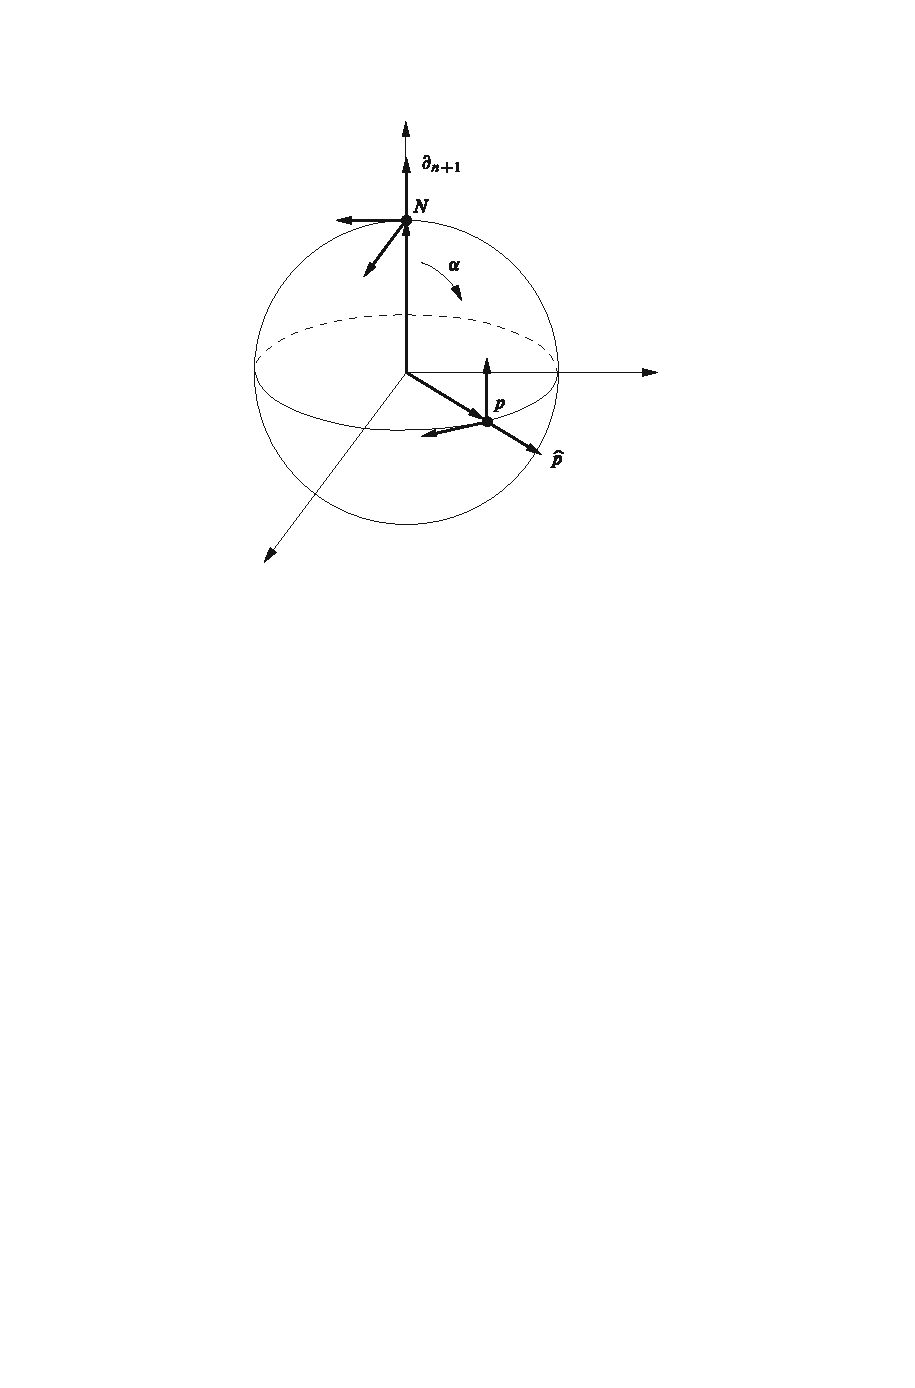
\includegraphics{pictures/sphere-homogeneous}
\caption{Transitivity of $\O(n+1)$ on $\O(S^n(R))$.}
\end{figure}
Another important feature of the round metrics---one that is much less evident than their 
symmetry---is that they bear a certain close relationship to the Euclidean metrics, which we now 
describe. Two metrics $g_1$ and $g_2$ on a manifold $M$ are said to be \textbf{conformally related} (or \textbf{pointwise conformal} or just \textbf{conformal}) to each other if there is a positive function $f\in C^\infty(M)$ such that $g_2=fg_1$. Given two Riemannian manifolds $(M,g)$ and $(\widetilde{M},\tilde{g})$, a diffeomorphism $\varphi:M\to\widetilde{M}$ is called a \textbf{conformal diffeomorphism} (or a \textbf{conformal transformation}) if it pulls $\tilde{g}$ back to a metric that is conformal to $g$:
\[\varphi^*\tilde{g}=fg\]
for some $f\in C^{\infty}(M)$. The following proposition shows that conformal diffeomorphisms 
are the same as \textbf{angle-preserving diffeomorphisms}.
\begin{proposition}
Let $g_1$ and $g_2$ be two Riemannian metrics on $M$. Then $g_1$ and $g_2$ are conformal if and only if they define the same angles. Therefore, a diffeomorphism is a conformal equivalence if and only if it preserves angles.
\end{proposition}
\begin{proof}
One direction is clear. Now assume that $g_1$ and $g_2$ define the same angle. Let $(E_i)$ be a local orthonormal frame for $g_1$, and consider the $g_2$-angle between $E_i$ and $(\cos\theta)E_i+(\sin\theta)E_j$. Since $g_1$ and $g_2$ define the same angle, we have $\langle E_i,E_j\rangle_{g_2}=0$ for $i\neq j$, and thus
\begin{align*}
\cos\theta&=\frac{\langle E_i,(\cos\theta)E_i+(\sin\theta)E_j\rangle_{g_2}}{|E_i|_{g_2}\cdot|(\cos\theta)E_i+(\sin\theta)E_j|_{g_2}}\\
&=\cos\theta\cdot\frac{|E_i|_{g_2}}{\sqrt{\cos^2\theta|E_i|_{g_2}^2+\sin^2\theta|E_j|_{g_2}^2}}.
\end{align*}
This then implies that $|E_i|_{g_2}=|E_j|_{g_2}$. Since $i,j$ are arbitrary, we conclude that $g_2=fg_1$ for a function $f:M\to\R$. Since $g_2$ is smooth, it follows that $f$ is smooth. Therefore $g_1$ and $g_2$ are conformal.
\end{proof}
Two Riemannian manifolds are said to be \textbf{conformally equivalent} if there is a conformal diffeomorphism between them. A Riemannian manifold $(M,g)$ is said to be \textbf{locally conformally flat} if every point of $M$ has a neighborhood that is conformally equivalent to an open set in $(\R^n,\widebar{g})$.\par
A conformal equivalence between $\R^n$ and $S^n(R)$ minus a point is provided by stereographic projection from the north pole. This is given by the following formula
\[\sigma(\xi,\tau)=u=\frac{R\xi}{R-\tau}\]
\begin{figure}[htbp]
\centering
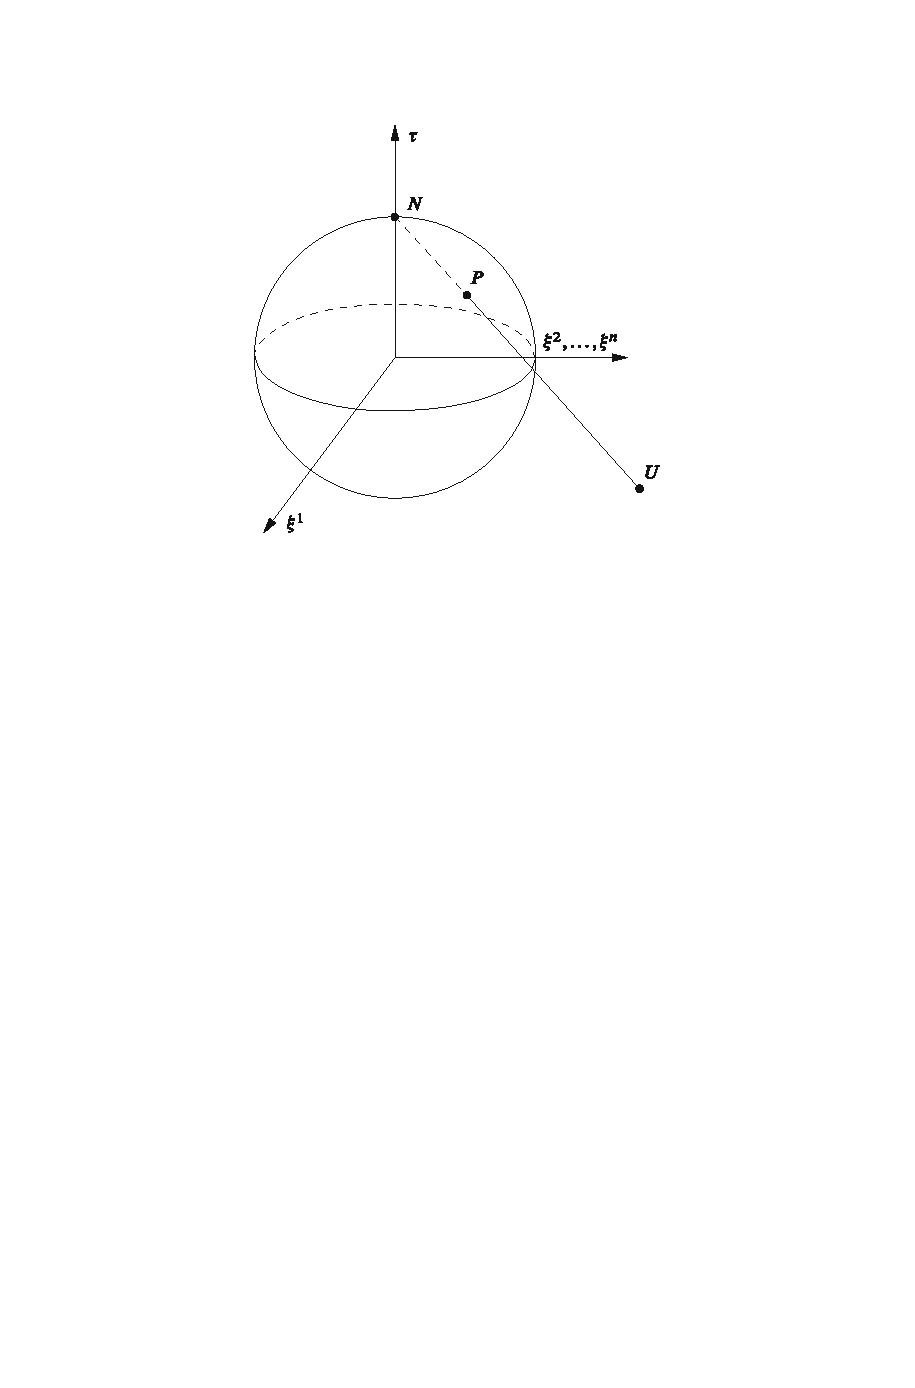
\includegraphics{pictures/stereographic-projection}
\caption{Stereographic projection.}
\end{figure}

It follows from this formula that $\sigma$ is defined and smooth on all of $S^n(R)-\{N\}$. The easiest way to see that it is a diffeomorphism is to compute its inverse:
\[\sigma^{-1}(u)=(\xi,\tau)=\Big(\frac{2R^2u}{|u|^2+R^2},R\frac{|u|^2-R^2}{|u|^2+R^2}\Big).\]
\begin{proposition}
Stereographic projection is a conformal diffeomorphism between $S^n(R)-\{N\}$ and $\R^n$.
\end{proposition}
\begin{proof}
The inverse map $\sigma^{-1}$ is a smooth parametrization of $S^n(R)-\{N\}$, so we can use it to compute the pullback metric. Using the usual technique of substitution to compute pullbacks, we obtain the following coordinate representation of $\mathring{g}_R$ in stereographic coordinates:
\[(\sigma^{-1})^*\mathring{g}_R=(\sigma^{-1})^*\widebar{g}=\sum_i\Big(d\Big(\frac{2R^2u^i}{|u|^2+R^2}\Big)\Big)^2+\Big(d\Big(R\frac{|u|^2-R^2}{|u|^2+R^2}\Big)\Big)^2.\]
If we expand each of these terms individually, we get
\begin{align*}
d\Big(\frac{2R^2u^i}{|u|^2+R^2}\Big)&=\frac{2R^2du^i}{|u|^2+R^2}-\frac{4R^2u^i\sum_ju^jdu^j}{(|u|^2+R^2)^2}\\
d\Big(R\frac{|u|^2-R^2}{|u|^2+R^2}\Big)&=\frac{2R\sum_ju^jdu^j}{|u|^2+R^2}-\frac{2R(|u|^2-R^2)\sum_ju^jdu^j}{(|u|^2+R^2)^2}=\frac{4R^3\sum_ju^jdu^j}{(|u|^2+R^2)^2}.
\end{align*}
Therefore,
\begin{align*}
(\sigma^{-1})^*\mathring{g}_R&=\frac{4R^4\sum_i(du^i)^2}{(|u|^2+R^2)^2}-\frac{16R^4(\sum_ju^jdu^j)^2}{(|u|^2+R^2)^3}+\frac{16R^4|u|^2(\sum_ju^jdu^j)^2}{(|u|^2+R^2)^4}+\frac{16R^6(\sum_ju^jdu^j)^2}{(|u|^2+R^2)^4}\\
&=\frac{4R^4\sum_i(du^i)^2}{(|u|^2+R^2)^2}.
\end{align*}
In other words,
\[(\sigma^{-1})^*\mathring{g}_R=\frac{4R^4}{(|u|^2+R^2)^2}\widebar{g},\]
where $\widebar{g}$ now represents the Euclidean metric on $\R^n$, and so $\sigma$ is a conformal
diffeomorphism.
\end{proof}
\begin{corollary}
Each sphere with a round metric is locally conformally flat.
\end{corollary}
\begin{proof}
Stereographic projection gives a conformal equivalence between a neighborhood of any point except the north pole and Euclidean space; applying a suitable rotation and then stereographic projection (or stereographic projection from the south pole), we get such an equivalence for a neighborhood of the north pole as well.
\end{proof}
\subsection{Hyperbolic spaces}
Our third class of model Riemannian manifolds is perhaps less familiar than the other two. For each $n\geq 1$ and each $R>0$ we will define a frame-homogeneous Riemannian manifold $\H^n(R)$, called \textbf{hyperbolic space of radius $\bm{R}$}. There are four equivalent models of the hyperbolic spaces, each of which is useful in certain contexts. In the next theorem, we introduce all of them and show that they are isometric.
\begin{theorem}\label{Hyperbolic space}
Let $n$ be an integer greater than $1$. For each fixed $R>0$, the following Riemannian manifolds 
are all mutually isometric.
\begin{itemize}
\item[(a)] (\textbf{Hyperboloid model}) $\H^n(R)$ is the submanifold of Minkowski space $\R^{n,1}$ 
defined in standard coordinates $(\xi,\tau)$ as the "upper sheet" $\{\tau>0\}$ of the two-sheeted 
hyperboloid $|\xi|^2-\tau^2=-R^2$, with the induced metric $\breve{g}^1_R=\iota^*\widebar{q}$ where 
$\iota:\H^n(R)\to\R^{n,1}$ is inclusion, and $\widebar{q}$ is the Minkowski metric:
\begin{align}\label{Hyperbolic space metric-1}
\widebar{q}=(d\xi^1)^2+\cdots+(d\xi^n)^2-(d\tau)^2.
\end{align}
\item[(b)] (\textbf{Beltrami-Klein model}) $\K^n(R)$ is the ball of radius $R$ centered at the
origin in $\R^n$, with the metric given in coordinates $(w^1,\dots,w^n)$ by
\begin{align}\label{Hyperbolic space metric-2}
\breve{g}^2_R=R^2\frac{(dw^1)^2+\cdots+(dw^n)^2}{R^2-|w|^2}+R^2\frac{(w^1dw^1+\cdots+w^ndw^n)^2}{(R^2-|w|^2)^2}.
\end{align}
\item[(c)] (\textbf{Poincar\'e ball model)}) $\B^n(R)$ is the ball of radius $R$ centered at 
the origin in $\R^n$, with the metric given in coordinates $(u^1,\dots,u^n)$ by
\begin{align}\label{Hyperbolic space metric-3}
\breve{g}^3_R=4R^4\frac{(du^1)^2+\cdots+(du^n)^2}{(R^2-|u|^2)^2}.
\end{align}
\item[(d)] (\textbf{Poincar\'e half-space model}) $\mathbb{U}^n(R)$ is the upper half-space in $\R^n$ 
defined in coordinates $(x^1,\dots,x^{n-1},y)$ by $\mathbb{U}^n(R)=\{(x,y):y>0\}$, endowed with 
the metric
\begin{align}\label{Hyperbolic space metric-4}
\breve{g}^4_R=R^2\frac{(dx^1)^2+\cdots+(dx^{n-1})^2+(dy)^2}{y^2}
\end{align}
\end{itemize}
\end{theorem}
\begin{proof}
Let $R>0$ be given. We need to verify that $\H^n(R)$ is actually a Riemannian submanifold of 
$\R^{n,1}$, or in other words that $\breve{g}^1_R$ is positive definite. One way to do this 
is to show, as we will below, that it is the pullback of $\breve{g}^2_R$ or $\breve{g}^3_R$ 
(both of which are manifestly positive definite) by a diffeomorphism. Alternatively, here 
is a direct proof using some of the theory of submanifolds of pseudo-Riemannian manifolds.
\begin{figure}[htbp]
\centering
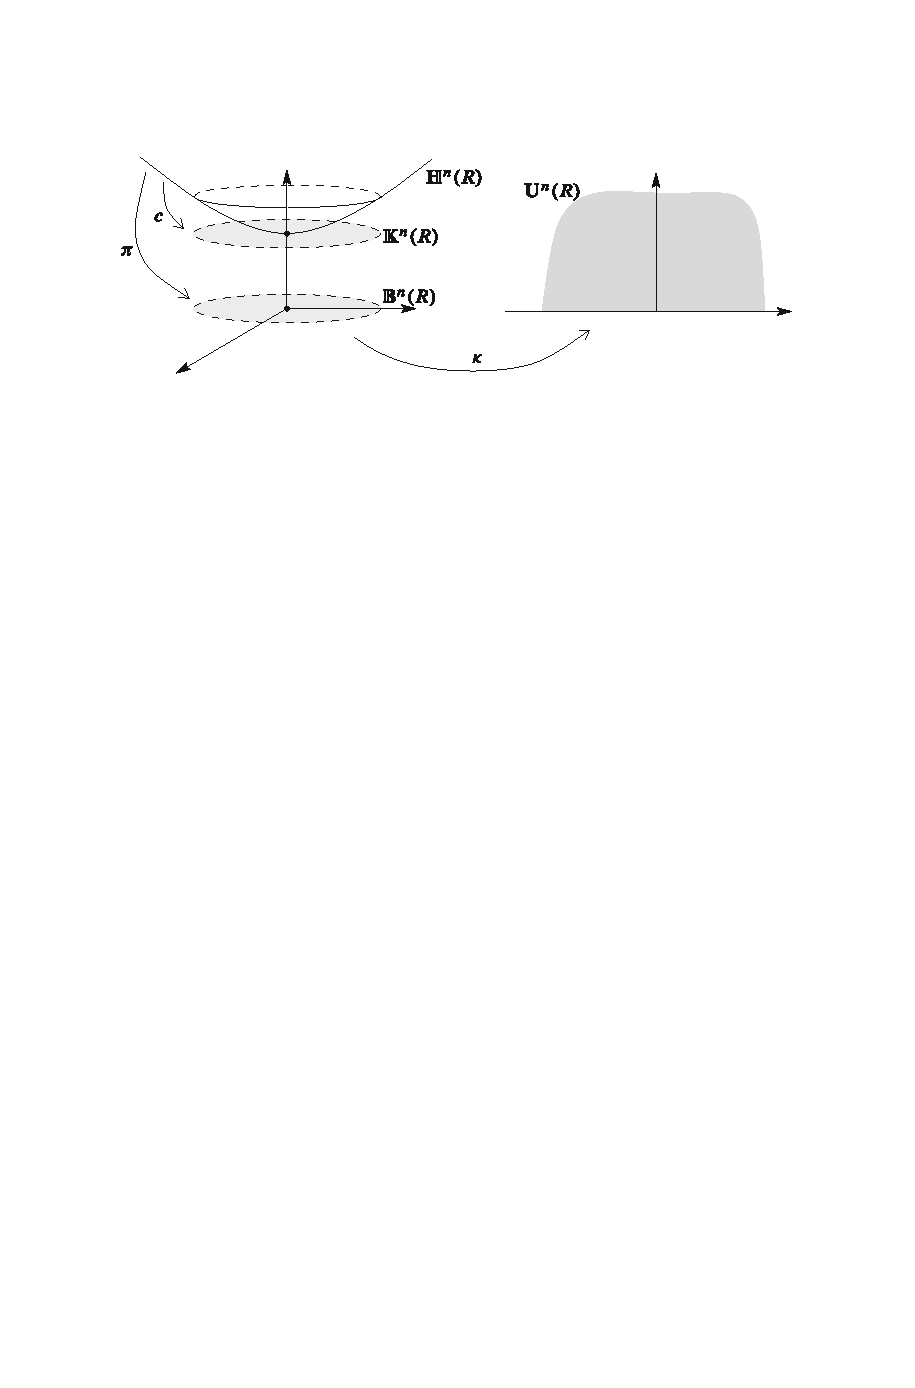
\includegraphics{pictures/hyperbolic-model}
\caption{Isometries among the hyperbolic models.}
\end{figure}

Note that $\H^n(R)$ is an open subset of a level set of the smooth function $f:\R^{n,1}\to\R$ given 
by $f(\xi,\tau)=(\xi^1)^2+\cdots+(\xi^n)^2-\tau^2$. We have
\[df=2\xi^1d\xi^2+\cdots+2\xi^nd\xi^n-2\tau d\tau,\]
and therefore the gradient of $f$ with respect to $\widebar{q}$ is given by
\begin{align}\label{Hyperbolic space defining grad}
\grad f=2\xi^1\frac{\partial}{\partial \xi^1}+\cdots+2\xi^n\frac{\partial}{\partial \xi^n}+2\tau\frac{\partial}{\partial \tau}.
\end{align}Direct computation gives $\widebar{q}(\grad f,\grad f)=4(\sum_i(\xi^i)^2-\tau^2)=-4R^2<0$, therefore $\H^n(R)$ 
is a pseudo-Riemannian manifold of signature $(n,0)$, that is, a Riemannian manifold.\par
We will show that all four Riemannian manifolds are mutually isometric by defining isometries 
$c:\H^n(R)\to\K^n(R)$, $\pi:\H^n(R)\to\B^n(R)$ and $\kappa:\B^n(R)\to\mathrm{U}^n(R)$.\par
We begin with a geometric construction of a diffeomorphism called \textbf{central projection} from the hyperboloid to the ball, $c:\H^n(R)\to\K^n(R)$, which turns out to be an isometry between the two metrics given in (a) and (b). For any $P=(\xi,\tau)\in\R^{n,1}$, set $c(P)=w\in\K^n(R)$, where $W=(w,0)\in\R^{n,1}$ is the point where the line from the origin to $P$ intersects the hyperplane $\{(\xi,\tau):\tau=R\}$. Because $W$ 
is characterized as the unique scalar multiple of $P$ whose last coordinate is $R$, we have $W=RP/\tau$, and therefore $c(\xi,\tau)=R\xi/\tau$.\par
\begin{figure}[htbp]
\centering
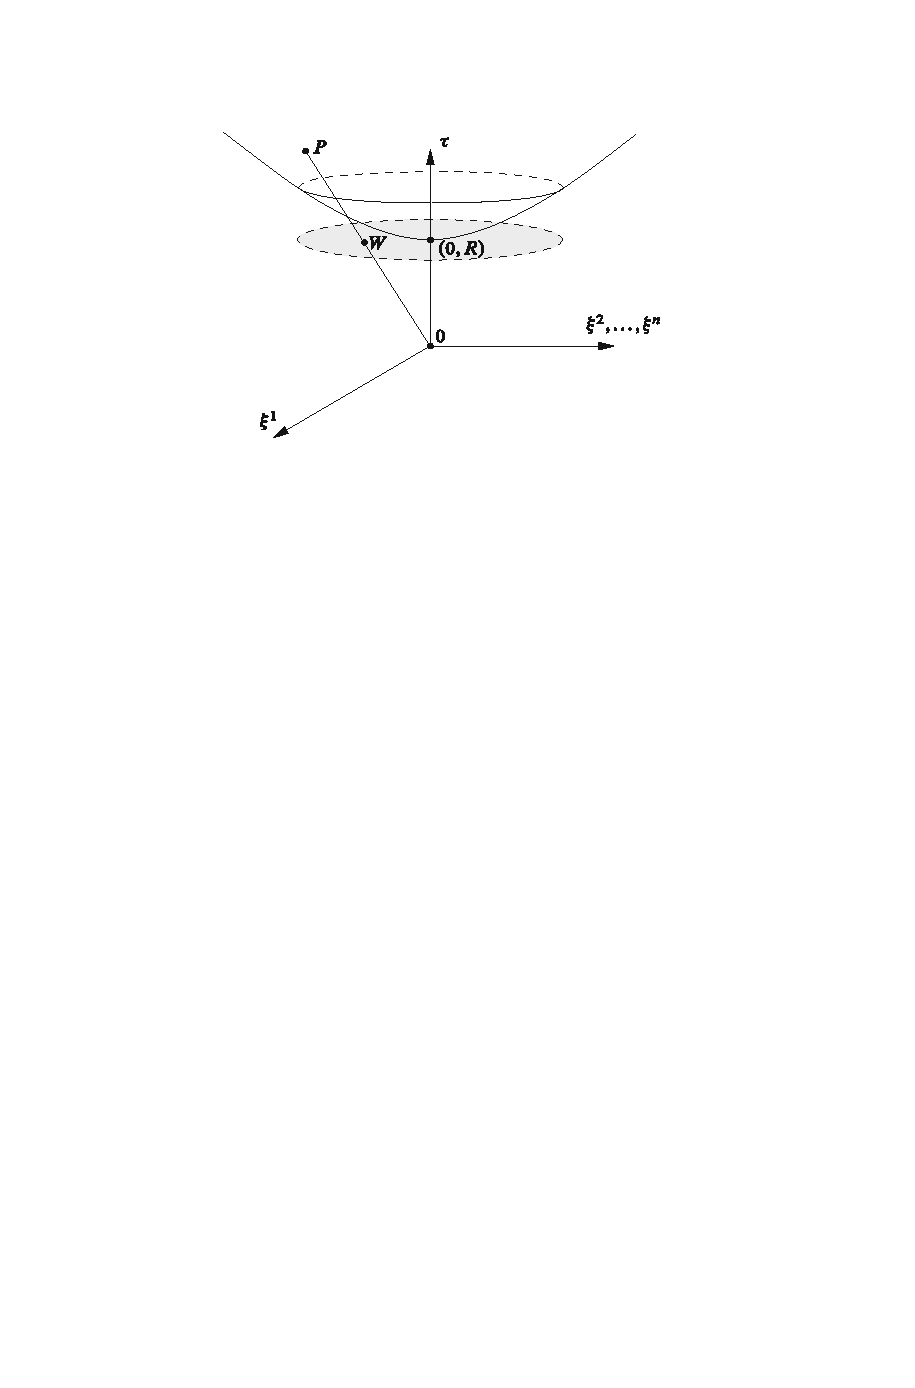
\includegraphics[width=180pt]{pictures/central-projection}
\caption{Central projection from the hyperboloid to the Beltrami-Klein model.}
\label{Hyperbolic central proj}
\end{figure}
The relation $|\xi|^2-\tau^2=-\R^2$ guarantees that $|c(\xi,\tau)|^2=R^2(1-R^2/\tau^2)<R^2$, so $c$ maps $\H^n(R)$ into $\K^n(R)$. To show that $c$ is a diffeomorphism, we determine its inverse map. Let $w\in\K^n(R)$ be arbitrary. The unique positive scalar $\lambda$ such that the point $(\xi,\tau)=\lambda(w,R)$ lies on $\H^n(R)$ is characterized by $\lambda^2|w|^2-\lambda^2R^2=-R^2$, and therefore
\[\lambda=\frac{R}{\sqrt{R^2-|w|^2}}.\]
It follows that the following smooth map is an inverse for $c$:
\[c^{-1}(w)=(\xi,\tau)=\Big(\frac{Rw}{\sqrt{R^2-|w|^2}},\frac{R^2}{\sqrt{R^2-|w|^2}}\Big).\]
Thus $c$ is a diffeomorphism. To show that it is an isometry between $\breve{g}^1_R$ and $\breve{g}^2_R$, we use the fact that $\breve{g}^1_R$ is the metric induced from $\widebar{q}$, analogously to the computation we did for stereographic projection above. With $(\xi,\tau)$ defined above, we have
\begin{align*}
& d\xi^i=\frac{Rdw^i}{\sqrt{R^2-|w|^2}}+\frac{Rw^i\sum_jw^jdw^j}{(R^2-|w|^2)^{3/2}},\quad d\tau=\frac{R^2\sum_jw^jdw^j}{(R^2-|w|^2)^{3/2}}.
\end{align*}
It then follows that
\begin{align*}
(c^{-1})^*\breve{g}^1_R&=\sum_i(d\xi^i)^2-(d\tau)^2\\
&=\frac{R^2\sum_i(dw^i)^2}{R^2-|w|^2}+\frac{R^2|w|^2(\sum_jw^jdw^j)^2}{(R^2-|w|^2)^3}+\frac{2R^3(\sum_jw^jdw^j)^2}{(R^2-|w|^2)^2}-\frac{R^4(\sum_jw^jdw^j)^2}{(R^2-|w|^2)^3}\\
&=R^2\frac{\sum_i(dw^i)^2}{R^2-|w|^2}+R^2\frac{(\sum_jw^jdw^j)^2}{(R^2-|w|^2)^2}.
\end{align*}
Next we describe a diffeomorphism $\pi:\H^n(R)\to\B^n(R)$ from the hyperboloid to the ball, called \textbf{hyperbolic stereographic projection}, which is an isometry between the metrics of (a) and (c). Let $S\in\R^{n,1}$ denote the point $S=(0,\dots,0,-R)$. For any $P=(\xi,\tau)\in\H^n(R)\sub\R^{n,1}$, set $\pi(P)=u\in\B^n(R)$, where $U=(u,0)\in\R^{n,1}$ is the point where the line through $S$ and $P$ intersects the hyperplane $\{(\xi,\tau):\tau=0\}$. The point $U$ is characterized by $(U-S)=\lambda(P-S)$ for some nonzero scalar $\lambda$, so we get $\lambda=R/(R+\tau)$ 
and thus
\[\pi(\xi,\tau)=u=\frac{R\xi}{R+\tau},\]
which takes its values in $\B^n(R)$ because $|\pi(\xi,\tau)|^2=R^2(\tau^2-R^2)/(R+\tau)^2<R^2$. A computation similar to the ones before shows that the inverse map is
\[\pi^{-1}(u)=(\xi,\tau)=\Big(\frac{2R^2u}{R^2-|u|^2},R\frac{R^2+|u|^2}{R^2-|u|^2}\Big).\]
We will show that $(\pi^{-1})^*\breve{g}^1_R=\breve{g}^3_R$. The computation proceeds just as in the spherical case, with
\[d\xi^i=\frac{2R^2du^i}{R^2-|u|^2}+4R^2\frac{u^i\sum_ju^jdu^j}{(R^2-|u|^2)^2},\quad d\tau=\frac{4R^2\sum_ju^jdu^j}{(R^2-|u|^2)^2}\]
and therefore
\begin{align*}
(\pi^{-1})^*\breve{g}^1_R&=\frac{4R^2\sum_i(du^i)^2}{(R^2-|u|^2)^2}+\frac{16R^4(\sum_ju^jdu^j)^2}{(R^2-|u|^2)^3}+\frac{16R^4|u|^2\sum_ju^jdu^j}{(R^2-|u|^2)^4}-\frac{16R^6\sum_ju^jdu^j}{(R^2-|u|^2)^4}\\
&=4R^2\frac{\sum_i(du^i)^2}{(R^2-|u|^2)^2}=\breve{g}^3_R.
\end{align*}
\begin{figure}[htbp]
\centering
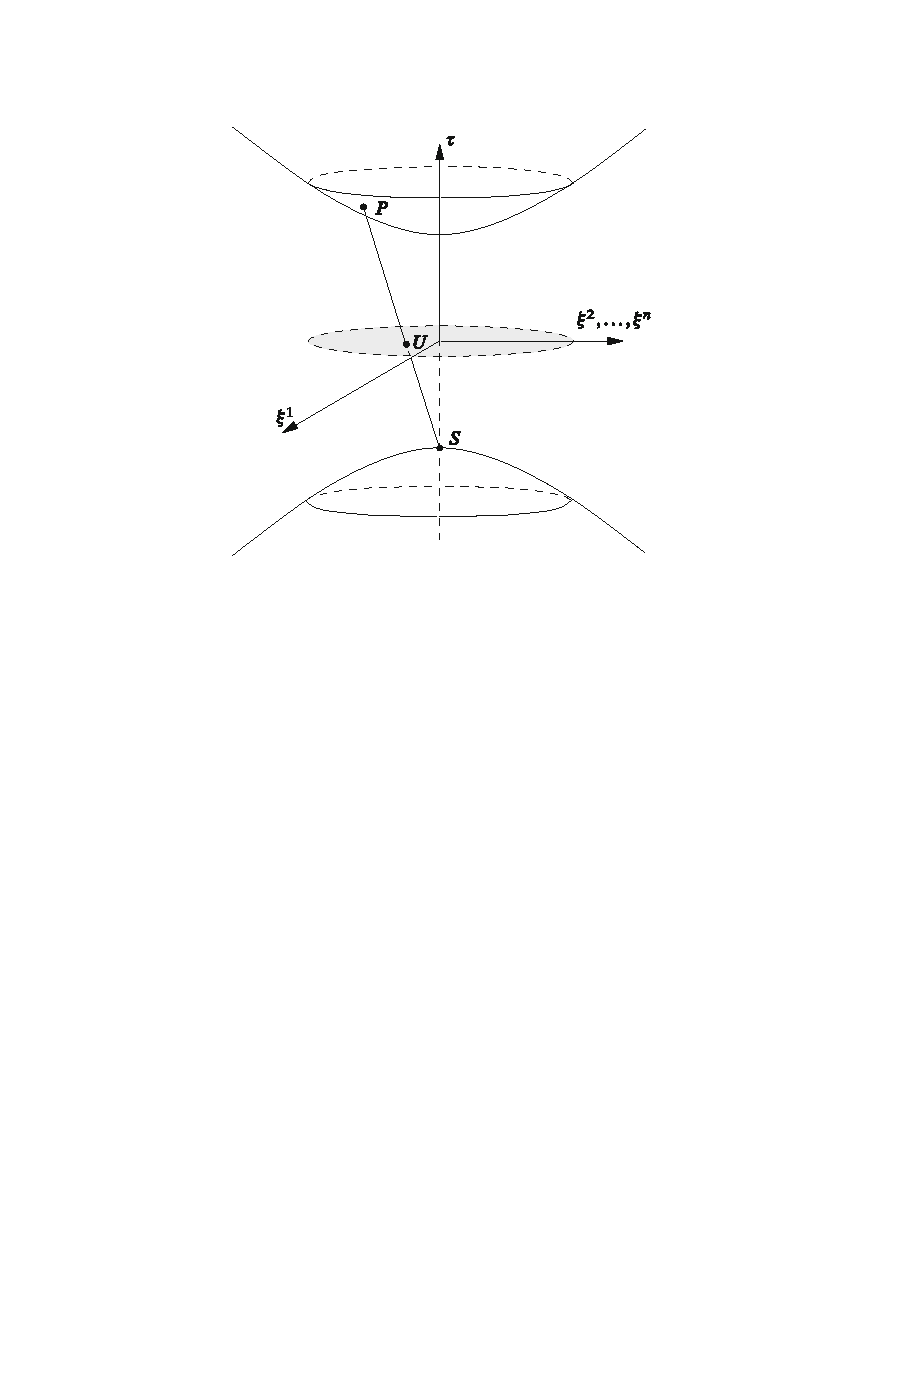
\includegraphics[width=160pt]{pictures/hyperbolic-stereographic-projection}
\caption{Hyperbolic stereographic projection.}
\label{Hyperbolic stereographic proj}
\end{figure}
Now we consider the Poincar\'e half-space model, by constructing an explicit diffeomorphism $\kappa:\mathbb{U}^n(R)\to\B^n(R)$.
In this case it is convenient to write the coordinates on the ball as $(u,v)=(u^1,\dots,u^{n-1},v)$. In the $2$-dimensional case, it is easy to write down in complex notation $w=u+iv$ and $z=x+iy$. It is a Mobious transformation:
\begin{align}\label{Hyperbolic space-1}
\kappa(z)=w=iR\frac{z-iR}{z+iR}.
\end{align}
Since $\kappa(iR)=0$, $\kappa(0)=-iR$ and $\kappa(\infty)=iR$, it is a complex-analytic diffeomorphism taking $\mathbb{U}^2(R)$ onto $\B^2(R)$. Separating $z$ into real and imaginary parts, we can also write this in real terms as
\[\kappa(x,y)=(u,v)=\Big(\frac{2R^2x}{|x|^2+(y+R)^2},R\frac{|x|^2+y^2-R^2}{|x|^2+(y+R)^2}\Big).\]
This same formula makes sense in any dimension $n$ if we interpret $x$ to mean $(x^1,\dots,x^{n-1})$, and it is easy to check that it maps the upper half-space $\{y>0\}$ into the ball of radius $R$. From 
the formula $(\ref{Hyperbolic space-1})$ we can construct the inverse of $\kappa$:
\[\kappa^{-1}(u,v)=(x,y)=\Big(\frac{2R^2u}{|u|^2+(v-R)^2},R\frac{R^2-|u|^2-v^2}{|u|^2+(v-R)^2}\Big),\]
so $\kappa$ is a diffeomorphism. We compute that
\begin{align*}
du^i=\frac{2R^2dx^i}{|x|^2+(y+R)^2}-\frac{4R^2x^i\sum_jx^jdx^j}{(|x|^2+(y+R)^2)^2}-\frac{4R^2x^i(y+R)dy}{(|x|^2+(y+R)^2)^2},
\end{align*}
and
\begin{align*}
dv&=\frac{2Rx^i\sum_jx^jdx^j}{|x|^2+(y+R)^2}-\frac{2R(|x|^2+y^2-R^2)\sum_jx^jdx^j}{(|x|^2+(y+R)^2)^2}\\
&\quad +\frac{2Ry(|x|^2+(y+R)^2)-2(y+R)(|x|^2+(y+R)^2)}{(|x|^2+(y+R)^2)^2}\\
&=\frac{4R^2(y+R)\sum_jx^jdx^j}{(|x|^2+(y+R)^2)^2}+\frac{2R^2((y+R)^2-|x|^2)dy}{(|x|^2+(y+R)^2)^2}.
\end{align*}
With these, we have (for simplicity, we set $\Delta:=|x|^2+(y+R)^2$)
\begin{align*}
&(du^1)^2+\cdots+(du^{n-1})^2+(dv)^2\\
&=\frac{4R^4\sum_i(dx^i)^2}{\Delta^2}+\frac{16R^4|x|^2(\sum_jx^jdx^j)^2}{\Delta^4}+\frac{16R^4|x|^2(y+R)^2(dy)^2}{\Delta^4}\\
&\quad -\frac{16R^4(\sum_jx^jdx^j)^2}{\Delta^3}-\frac{16R^4(y+R)(\sum_jx^jdx^j)dy}{\Delta^3}+\frac{32R^4|x|^2(y+R)(\sum_jx^jdx^j)dy}{\Delta^4}\\
&\quad +\frac{16R^4(y+R)^2(\sum_jx^jdx^j)^2}{\Delta^4}+\frac{4R^4[(y+R)^2-|x|^2]^2(dy)^2}{\Delta^4}\\
&\quad +\frac{16R^4(y+R)[(y+R)^2-|x|^2](\sum_jx^jdx^j)dy}{\Delta^4}\\
&=\frac{4R^2}{\Delta^2}\sum_i(dx^i)^2+(dy)^2\Big[\frac{16R^4|x|^2(y+R)^2}{\Delta^4}+\frac{4R^4[(y+R)^2-|x|^2]^2}{\Delta^4}\Big]\\
&\quad+(\sum_jx^jdx^j)^2\Big[\frac{16R^4|x|^2}{\Delta^4}-\frac{16R^4}{\Delta^3}+\frac{16R^4(y+R)^2}{\Delta^4}\Big]\\
&\quad +(\sum_jx^jdx^j)dy\Big[-\frac{16R^4(y+R)}{\Delta^3}+\frac{32R^4|x|^2(y+R)}{\Delta^4}+\frac{16R^4(y+R)[(y+R)^2-|x|^2]}{\Delta^4}\Big].
\end{align*}
Now we analyse the summands. First we have
\begin{align*}
&\frac{16R^4|x|^2(y+R)^2}{\Delta^4}+\frac{4R^4[(y+R)^2-|x|^2]^2}{\Delta^4}=\frac{4R^4}{\Delta^4}(4|x|^2(y+R)^2+[(y+R)^2-|x|^2]^2)\\
&=\frac{4R^4}{\Delta^4}[(y+R)^2+|x|^2]^2=\frac{4R^4}{\Delta^2}.
\end{align*}
Second, note that
\begin{align*}
\frac{16R^4|x|^2}{\Delta^4}-\frac{16R^4}{\Delta^3}+\frac{16R^4(y+R)^2}{\Delta^4}=\frac{16R^4}{\Delta^4}(|x|^2-\Delta+(y+R)^2)=0,
\end{align*}
and finally,
\begin{align*}
&-\frac{16R^4(y+R)}{\Delta^3}+\frac{32R^4|x|^2(y+R)}{\Delta^4}+\frac{16R^4(y+R)[(y+R)^2-|x|^2]}{\Delta^4}\\
&=\frac{16R^4(y+R)}{\Delta^4}(\Delta-2|x|^2+(y+R)^2-|x|^2)=0.
\end{align*}
Therefore we derive from our previous calculation that
\begin{align*}
(du^1)^2+\cdots+(du^{n-1})^2+(dv)^2=\frac{4R^4}{\Delta^2}((dx^1)^2+\cdots+(dx^{n-1})^2+(dy)^2).
\end{align*}
To end the verification, we observe that
\begin{align*}
|u|^2+v^2&=\frac{R^2}{\Delta^2}(4R^2|x|^2+(|x|^2+y^2-R^2)^2))\\
&=\frac{R^2}{\Delta^2}(|x|^4+y^2+R^2+2R^2|x|^2+2|x|^2y^2-2R^2y^2)\\
&=\frac{R^2}{\Delta^2}((|x|^2+y^2+R^2)^2-(2Ry)^2)\\
&=\frac{R^2(|x|^2+(y+R)^2)(|x|^2+(y-R)^2)}{\Delta^2}\\
&=\frac{R^2(|x|^2+(y-R)^2)}{\Delta}.
\end{align*}
and therefore
\[\frac{1}{(R^2-|(u,v)|^2)^2}=\frac{\Delta^2}{R^2(\Delta-|x|^2-(y-R)^2)^2}=\frac{\Delta^2}{16R^6y^2}.\]
Once this is established, we then get
\begin{align*}
\kappa^*\breve{g}^3_R&=\frac{4R^4}{(R^2-|(u,v)|^2)^2}((du^1)^2+\cdots+(du^{n-1})^2+(dv)^2)\\
&=\frac{4R^4\Delta^2}{16R^6y^2}\cdot\frac{4R^4}{\Delta^2}((dx^1)^2+\cdots+(dx^{n-1})^2+(dy)^2)\\
&=R^2\frac{(dx^1)^2+\cdots+(dx^{n-1})^2+(dy)^2}{y^2}\\
&=\breve{g}^4_R.
\end{align*}
This finishes the proof.
\end{proof}
We often use the generic notation $\H^n(R)$ to refer to any one of the Riemannian manifolds 
of Theorem~\ref{Hyperbolic space}, and $\breve{g}_R$ to refer to the corresponding metric; 
the special case $R=1$ is denoted by $(\H^n,\breve{g})$ and is called simply 
\textbf{hyperbolic space}, or in the $2$-dimensional case, the \textbf{hyperbolic plane}.\par
Because all of the models for a given value of $R$ are isometric to each other, when analyzing 
them geometrically we can use whichever model is most convenient for the application we have 
in mind. The next corollary is an example in which the Poincar\'e ball and half-space 
models serve best.
\begin{corollary}
Each hyperbolic space is locally conformally flat.
\end{corollary}
\begin{proof}
In either the Poincar\'e ball model or the half-space model, the identity map gives a 
global conformal equivalence with an open subset of Euclidean space.
\end{proof}
The symmetries of $\H^n(R)$ are most easily seen in the hyperboloid model. Let $\O(n,1)$ 
denote the group of linear maps from $\R^{n,1}$ to itself that preserve the Minkowski metric, 
called the $(n+1)$-dimensional Lorentz group. Note that each element of $\O(n,1)$ preserves 
the hyperboloid $\{|\xi|^2-\tau^2=-R^2\}$, which has two components determined by $\tau>0$ 
and $\tau<0$. We let $\O^+(n,1)$ denote the subgroup of $\O(n,1)$ consisting of maps that 
take the $\tau>0$ component of the hyperboloid to itself. (This is called the 
\textbf{orthochronous Lorentz group}, because physically it represents coordinate changes 
that preserve the forward time direction.) Then $\O^+(n,1)$ preserves $\H^{n}(R)$, and 
because it preserves $\widebar{q}$ it acts isometrically on $\H^n(R)$.
\begin{proposition}\label{hyperbolic frame homogeneous}
The group $\O^+(n,1)$ acts transitively on $\O(\H^n(R))$, and therefore $\H^n(R)$ is frame-homogeneous.
\end{proposition}
\begin{figure}[htbp]
\centering
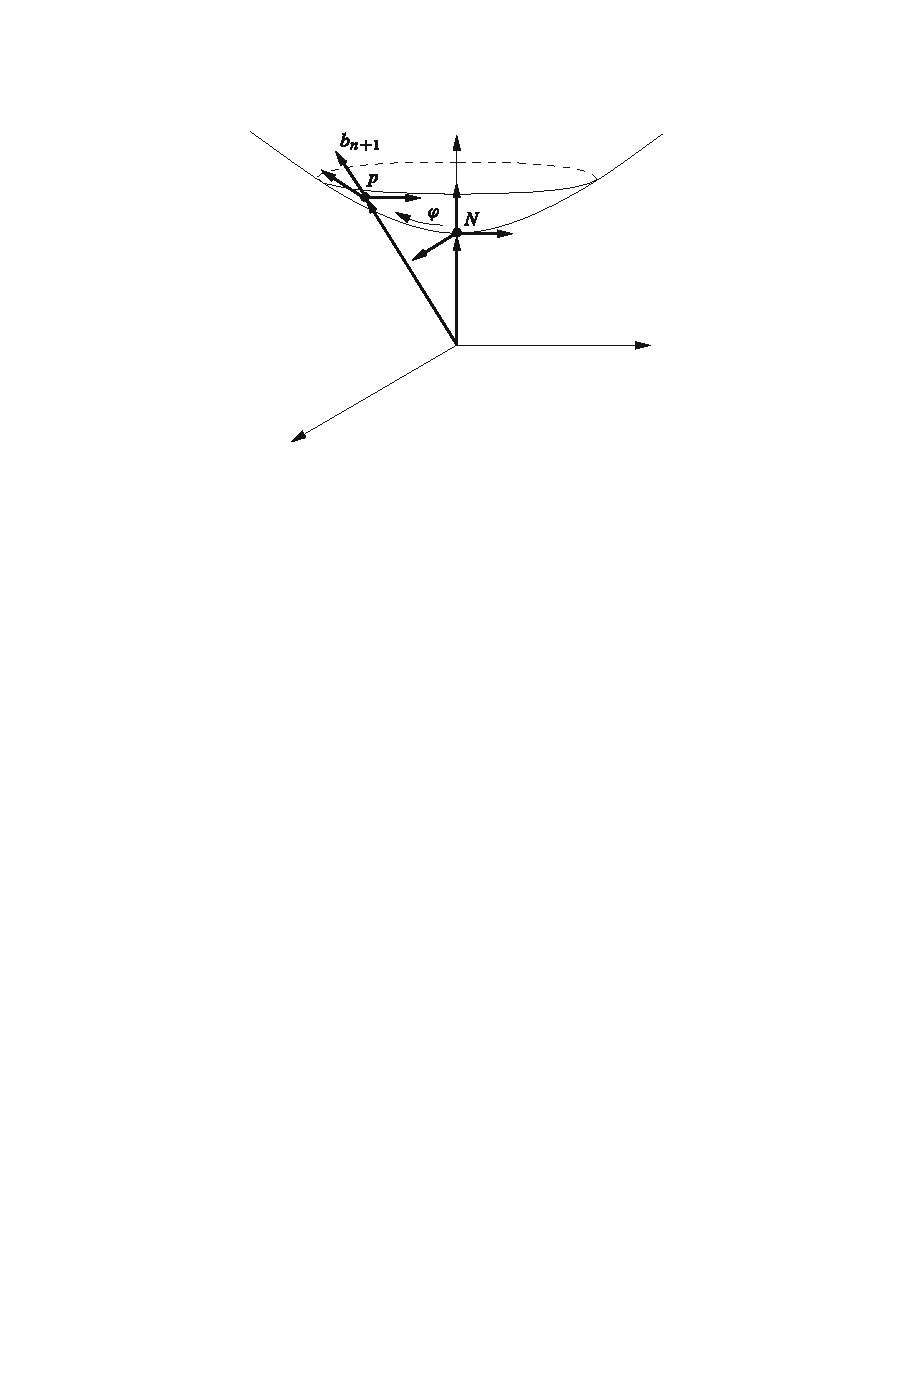
\includegraphics[width=180pt]{pictures/hyperbolic-space-homogeneous}
\caption{Frame homogeneity of $\H^n(R)$.}
\end{figure}
\begin{proof}
The argument is entirely analogous to the proof of Proposition~\ref{sphere frame homogeneous}, so we give only a sketch. Suppose $p\in\H^n(R)$ and $(e_i)$ is an orthonormal basis for $T_p\H^n(R)$. Identifying $p\in\R^{n,1}$ with an element of $T_p\R^{n,1}$ in the usual way, we can regard $\hat{p}=p/R$ as a $\widebar{q}$-unit vector in $T_p\R^{n,1}$, and $(\ref{Hyperbolic space defining grad})$ shows that it is a scalar multiple of the $\widebar{q}$-gradient of the defining function $f$ and thus is orthogonal to $T_p\H^n(R)$ with respect to $\widebar{q}$. Thus $(e_1,\dots,e_n,e_{n+1}=\hat{p})$ is a $\widebar{q}$-orthonormal basis for $\R^{n,1}$, and $\widebar{q}$ has the following expression in terms of the dual basis $(\beta^i)$:
\[\widebar{q}=(\beta^1)^2+\cdots+(\beta^n)^2-(\beta^{n+1})^2.\]
Thus the matrix whose columns are $(e_1,\dots,e_{n+1})$ is an element of $\O^+(n,1)$ sending the north pole $N=(0,\dots,0,R)$ to $p$ and $\partial_i$ to $e_i$.
\end{proof}
\subsection{Invariant metrics on Lie groups}
Lie groups provide us with another large class of homogeneous Riemannian manifolds. Let $G$ be 
a Lie group. A Riemannian metric $g$ on $G$ is said to be \textbf{left-invariant} if it is 
invariant under all left translations: $L^*_{\varphi}g=g$ for all $\varphi\in G$. Similarly, $g$ is 
\textbf{right-invariant} if it is invariant under all right translations, and \textbf{bi-invariant} 
if it is  both left- and right-invariant. The next lemma shows that left-invariant metrics 
are easy to come by.
\begin{lemma}\label{Riemann metric left-inv}
Let $G$ be a Lie group and let $\g$ be its Lie algebra of left-invariant vector fields.
\begin{itemize}
\item[(a)] A Riemannian metric $g$ on $G$ is left-invariant if and only if for all $X,Y\in\g$, 
the function $g(X,Y)$ is constant on $G$.
\item[(b)] The restriction map $g\mapsto g_e\in\Sigma^2(T_e^*G)$ together with the natural identification $T_eG\cong\g$ 
gives a bijection between left-invariant Riemannian metrics on $G$ and inner products on $g$.
\end{itemize}
\end{lemma}
\begin{proof}
We only need to prove (a). Note that, since $\g$ consists of left-invariant vector fields, for every $\varphi\in G$ we have
\begin{align*}
g(X,Y)_\varphi=g_{\varphi}(X_{\varphi},Y_{\varphi})=g_{\varphi}(d(L_\varphi)_e(X_e),d(L_{\varphi})_e(Y_e))=(L_\varphi^*g)_e(X_e,Y_e)=(L^*_{\varphi}g)(X,Y)_e.
\end{align*}
Therefore $g(X,Y)$ is constant on $G$ if $g$ is left-invariant.\par
Conversely, if $g(X,Y)$ is constant for all $X,Y\in\g$, we prove that $L_{\varphi}^*g=g$ for any $\varphi\in G$. In fact, fix $\varphi$ and let $\psi\in G$ and $u,v\in T_{\psi}G$, 
then we can choose $X,Y\in\g$ such that $X_{\psi}=u$, $Y_{\psi}=v$, so it follows that
\begin{align*}
(L_{\varphi}^*g)_{\psi}(u,v)&=(L_{\varphi}^*g)_{\psi}(X,Y)_{\psi}\\
&=g_{\varphi\psi}(d(L_{\varphi})_{\psi}(X_{\psi}),d(L_{\varphi})_{\psi}(Y_{\psi}))\\
&=g_{\varphi\psi}(X_{\varphi\psi},Y_{\varphi\psi})\\
&=g(X,Y)_{\varphi\psi}\\
&=g(X,Y)_{\psi}.
\end{align*}
This then implies $L_{\varphi}^*g=g$, so $g$ is left-invariant.
\end{proof}
Thus all we need to do to construct a left-invariant metric is choose any inner product on 
$g$, and define a metric on $G$ by applying that inner product to left-invariant vector 
fields. Right-invariant metrics can be constructed in a similar way using right-invariant 
vector fields. Since a Lie group acts transitively on itself by either left or right 
translation, every left-invariant or right-invariant metric is homogeneous.\par
Much more interesting are the bi-invariant metrics. Fortunately, there is a complete answer 
to the question of which Lie groups admit bi-invariant metrics.\par
We begin with a proposition that shows how to determine whether a given leftinvariant 
metric is bi-invariant, based on properties of the adjoint representation of the group. 
Recall that this is the representation $\Ad:G\to\GL(\g)$ given by 
$\Ad(\varphi)=(C_{\varphi})_*:\g\to\g$, where $C_\varphi$ is the automorphism defined by 
conjugation: $C_{\varphi}(\psi)=\varphi\psi\varphi^{-1}$.
\begin{proposition}\label{Riemann metric bi-inv iff}
Let $G$ be a Lie group and $\g$ its Lie algebra. Suppose $g$ is a left-invariant Riemannian 
metric on $G$, and let $\langle\cdot\,,\cdot\rangle$ denote the corresponding inner product 
on $\g$ as in Lemma~\ref{Riemann metric left-inv}. Then $g$ is bi-invariant if and only if 
$\langle\cdot\,,\cdot\rangle$ is invariant under the action of $\Ad(G)\sub\GL(\g)$, in the 
sense that $\langle\Ad(\varphi)X,\Ad(\varphi)Y\rangle=\langle X,Y\rangle$ for all $X,Y\in\g$ 
and $\varphi\in G$.
\end{proposition}
\begin{proof}
We begin the proof with some preliminary computations. Suppose $g$ is left-invariant and 
$\langle\cdot\,,\cdot\rangle$ is the associated inner product on $g$. Let $\varphi\in G$ be 
arbitrary, and note that $C_\varphi$ is the composition of left multiplication by $\varphi$ 
followed by right multiplication by $\varphi^{-1}$. Thus for every $X\in\g$, left-invariance 
implies $(R_{\varphi^{-1}})_*X=(R_{\varphi^{-1}})_*(L_{\varphi})_*X=(C_{\varphi})_*X=\Ad(\varphi)X$. 
Therefore, for all $\psi\in G$ and $X,Y\in\g$, we have
\begin{align*}
((R_{\varphi^{-1}})^*g)_{\psi}(X_{\psi},Y_{\psi})&=g_{\psi\varphi^{-1}}\big(((R_{\varphi^{-1}})_*X)_{\psi\varphi^{-1}},((R_{\varphi^{-1}})_*Y)_{\psi\varphi^{-1}}\big)\\
&=g_{\psi\varphi^{-1}}\big(\Ad(\varphi)X)_{\psi\varphi^{-1}},\Ad(\varphi)Y)_{\psi\varphi^{-1}}\big)\\
&=\langle\Ad(\varphi)X,\Ad(\varphi)Y\rangle_{\psi}.
\end{align*}
Now assume that $\langle\cdot\,,\cdot\rangle$ is invariant under $\Ad(G)$. Then the expression 
on the last line above is equal to $\langle X,Y\rangle_{\psi}=g_{\psi}(X_{\psi},Y_{\psi})$, which 
shows that $(R_{\varphi^{-1}})^*g=g$. Since this is true for all $\varphi\in G$, it follows that 
$g$ is bi-invariant.\par
Conversely, assuming that $g$ is bi-invariant, we have $(R_{\varphi^{-1}})^*g=g$ for each $\varphi\in G$, 
so the above computation yields
\[\langle X,Y\rangle_{\psi}=g_{\psi}(X_{\psi},Y_{\psi})=((R_{\varphi^{-1}})^*g)_{\psi}(X_{\psi},Y_{\psi})=\langle\Ad(\varphi)X,\Ad(\varphi)Y\rangle_{\psi},\]
which shows that $\langle\cdot\,,\cdot\rangle$ is $\Ad(G)$-invariant.
\end{proof}
In order to apply the preceding proposition, we need a lemma about finding invariant inner 
products on vector spaces. Recall that for every finite-dimensional real vector space $V$, 
$GL(V)$ denotes the Lie group of all invertible linear maps from $V$ to itself. If $H$ is a 
subgroup of $\GL(V)$, an inner product $\langle\cdot\,,\cdot\rangle$ on $V$ is said to be 
\textbf{$\bm{H}$-invariant} if $\langle hx,hy\rangle=\langle x,y\rangle$ for all $x,y\in V$ 
and $h\in H$.
\begin{lemma}\label{inner prod inv iff}
Suppose $V$ is a finite-dimensional real vector space and $H$ is a subgroup of $\GL(V)$. 
There exists an $H$-invariant inner product on $V$ if and only if $H$ has compact closure 
in $\GL(V)$.
\end{lemma}
\begin{proof}
Assume first that there exists an $H$-invariant inner product $\langle\cdot\,,\cdot\rangle$ 
on $V$. This implies that $H$ is contained in the subgroup $\O(V)\sub\GL(V)$ consisting of 
linear isomorphisms of $V$ that are orthogonal with respect to this inner product. Choosing an 
orthonormal basis of $V$ yields a Lie group isomorphism between $\O(V)$ and $\O(n)\sub\GL_n(\R)$ 
(where $n=\dim V$), so $\O(V)$ is compact; and the closure of $H$ is a closed subset of this 
compact group, and thus is itself compact.\par
Conversely, suppose $H$ has compact closure in $\GL(V)$, and let $K$ denote the closure. Then 
by Proposition~\ref{topo subgroup closure} $K$ is also a subgroup, and thus it is a Lie group 
by the closed subgroup theorem. Let $\langle\cdot\,,\cdot\rangle$ be an arbitrary inner 
product on $V$, and let $\mu$ be a right-invariant volume form on $K$ (for example, the 
volume form of some right-invariant metric on $K$). Then define a new inner product 
$(\cdot\,,\cdot)$ on $V$ by
\[(x,y)=\int_K\langle kx,ky\rangle\mu.\]
It follows directly from the definition that $(\cdot\,,\cdot)$ is symmetric and bilinear 
over $\R$. For each nonzero $x\in V$, we have $\langle kx,kx\rangle>0$ everywhere on $K$, so $(x,y)>0$, 
showing that $(\cdot\,,\cdot)$ is indeed an inner product.\par
To see that it is invariant under $K$, let $k_0\in K$ be arbitrary. Then for all $x,y\in V$ and 
$k\in K$, we have
\begin{align*}
(k_0x,k_0y)&=\int_K\langle kk_0x,kk_0y\rangle\mu\\
&=\int_KR_{k_0}^*(\langle kx,ky\rangle\mu)\\
&=\int_K\langle kx,ky\rangle\mu=(x,y).
\end{align*}
Thus $(\cdot\,,\cdot)$ is $K$-invariant, and it is also $H$-invariant because $H\sub K$.
\end{proof}
\begin{theorem}\label{Riemann metric bi-inv exist}
Let $G$ be a Lie group and $g$ its Lie algebra. Then $G$ admits a bi-invariant metric if 
and only if $\Ad(G)$ has compact closure in $\GL(\g)$.
\end{theorem}
The most important application of the preceding theorem is to compact groups.
\begin{corollary}\label{Riemann metric bi-inv compact group}
Every compact Lie group admits a bi-invariant Riemannian metric.
\end{corollary}
\begin{proof}
If $G$ is compact, then $\Ad(G)$ is a compact subgroup of $\GL(\g)$ because $\Ad:G\to\GL(\g)$ 
is continuous.
\end{proof}
Another application is to prove that certain Lie groups do not admit bi-invariant 
metrics. One way to do this is to note that if $\Ad(G)$ has compact closure in $\GL(\g)$, 
then every orbit of $\Ad(G)$ must be a bounded subset of $\g$ with respect to any choice of 
norm, because it is contained in the image of the compact set $\widebar{\Ad(G)}$ under a 
continuous map of the form $\varphi\mapsto\varphi(X_0)$ from $\GL(\g)$ to $\g$. Thus if one 
can find an element $X_0\in\g$ and a subset $S\sub G$ such that the elements of the form 
$\Ad(\varphi)X_0$ are unbounded in $\g$ for $\varphi\in S$, then there is no bi-invariant 
metric.\par
Here are some examples.
\begin{example}[\textbf{Invariant Metrics on Lie Groups}]
\mbox{}
\begin{itemize}
\item[(a)] Every left-invariant metric on an abelian Lie group is bi-invariant, because 
the adjoint representation is trivial. Thus the Euclidean metric on $\R^n$ and the flat 
metric on $T^n$ are both bi-invariant.
\item[(b)] If a metric $g$ on a Lie group $G$ is left-invariant, then the induced metric 
on every Lie subgroup $H\sub G$ is easily seen to be left-invariant. Similarly, if $g$ is
bi-invariant, then the induced metric on $H$ is bi-invariant.
\item[(c)] The Lie group $\SL_2(\R)$ admits many left-invariant metrics, but no bi-invariant 
ones. To see this, recall that the Lie algebra of $\SL_2(\R)$ is isomorphic to the algebra 
$\sl(2,\R)$ of trace-free $2\times 2$ matrices, and the adjoint representation is given by 
$\Ad(A)X=AXA^{-1}$. If we let $X_0=(\begin{smallmatrix}
0&1\\
0&0
\end{smallmatrix})\in\sl(2,\R)$ and $A_c=\begin{smallmatrix}
c&0\\
0&1/c
\end{smallmatrix}\in\SL_2(\R)$ for $c>0$, then $\Ad(A_c)X_0=(\begin{smallmatrix}
0&c^2\\
0&0
\end{smallmatrix})$, which is unbounded as $c\to+\infty$. Thus the orbit of $X_0$ is not 
contained in any compact subset, which implies that there is no bi-invariant metric on 
$\SL_2(\R)$. A similar argument shows that $\SL_n(\R)$ admits no bi-invariant metric for 
any $n\geq 2$. In view of (b) above, this shows also that $\GL_n(\R)$ admits no bi-invariant 
metric for $n\geq 2$. (Of course, $\GL_1(\R)$ does admit bi-invariant metrics because it is 
abelian.)
\item[(d)] With $S^3$ regarded as a submanifold of $\C^2$, the map 
\[(w,z)\mapsto\begin{pmatrix}
w&z\\
-\widebar{z}&\widebar{w}
\end{pmatrix}\]
gives a diffeomorphism from $S^3$ to $\SU(2)$. Under the inverse of this map, the round metric 
on $S^3$ pulls back to a bi-invariant metric on $\SU(2)$.
\end{itemize}
\item[(e)] Let $\o(n)$ denote the Lie algebra of $\O(n)$, identified with the algebra of skew 
symmetric $n\times n$ matrices, and define a bilinear form on $\o(n)$ by
\[\langle A,B\rangle=\tr(A^TB).\]
This is an $\Ad$-invariant inner product, and thus determines a bi-invariant Riemannian metric 
on $\O(n)$.
\item[(f)] Let $\mathbb{U}^n$ be the upper half-space as defined in Theorem~\ref{Hyperbolic space}. 
We can regard $\mathbb{U}^n$ as a Lie group by identifying each point $(x,y)=(x^1,\dots,x^{n-1},y)\in\mathbb{U}^n$ 
with an invertible $n\times n$ matrix as follows:
\[(x,y)\longleftrightarrow\begin{pmatrix}
I_{n-1}&0\\
x^T&y
\end{pmatrix}\]
Then the hyperbolic metric $\breve{g}^4_R$ is left-invariant on $\mathbb{U}^n$ but not 
right-invariant.
\item[(g)] For $n\geq 1$, the $(2n+1)$-dimensional \textbf{Heisenberg group} is the Lie subgroup $H^n\sub\GL_{n+2}(\R)$ 
defined by
\[H_n=\Bigg\{\begin{pmatrix}
1&x^T&z\\
0&1&y\\
0&0&1
\end{pmatrix}:x,y\in\R^n,z\in\R\Bigg\},\]
where $x$ and $y$ are treated as column matrices. These are the simplest examples of \textbf{nilpotent 
Lie groups}. There are many left-invariant metrics on $H_n$, but no bi-invariant ones.
\item[(h)] Our last example is a group that plays an important role in the classification of $3$-manifolds. Let $\mathrm{Sol}$ denote the following $3$-dimensional 
Lie subgroup of $\GL_3(\R)$:
\[\mathrm{Sol}=\Bigg\{\begin{pmatrix}
e^z&0&x\\
0&e^{-z}&y\\
0&0&1
\end{pmatrix}:x,y,z\in\R\Bigg\}.\]
This group is the simplest non-nilpotent example of a \textbf{solvable Lie group}. Like the 
Heisenberg groups, Sol admits left-invariant metrics but not bi-invariant ones.
\end{example}
\subsection{Other homogeneous Riemannian manifolds}
There are many homogeneous Riemannian manifolds besides the frame-homogeneous ones and the 
Lie groups with invariant metrics. To identify other examples, it is natural to ask the 
following question: If $M$ is a smooth manifold endowed with a smooth, transitive action 
by a Lie group $G$ (called a homogeneous $G$-space or just a homogeneous space), is there a 
Riemannian metric on $M$ that is invariant under the group action?\par
The next theorem gives a necessary and sufficient condition for existence of an invariant 
Riemannian metric that is usually easy to check.
\begin{proposition}[\textbf{Existence of Invariant Metrics on Homogeneous Spaces}]\label{Riemann G-inv metric}
Suppose $G$ is a Lie group and $M$ is a homogeneous $G$-space. Let $p_0$ be a point in $M$, and 
let $I_{p_0}G_{p_0}\to\GL(T_{p_0}M)$ denote the isotropy representation at $p_0$. There exists 
a $G$-invariant Riemannian metric on $M$ if and only if $I_{p_0}(G_{p_0})$ has compact 
closure in $\GL(T_{p_0}M)$.
\end{proposition}
\begin{proof}
Assume first that $g$ is a $G$-invariant metric on $M$. Then the inner product $g_{p_0}$ on 
$T_{p_0}M$ is invariant under the isotropy representation, so it follows from Lemma~\ref{inner prod inv iff} 
that $I_{p_0}(G_{p_0})$ has compact closure in $\GL(T_{p_0}M)$.\par
Conversely, assume that $I_{p_0}(G_{p_0})$ has compact closure in $\GL(T_{p_0}M)$. Lemma~\ref{inner prod inv iff} 
shows that there is an inner product $g_{p_0}$ on $T_{p_0}M$ that is invariant under the 
isotropy representation. For arbitrary $p\in M$, we define an inner product $g_p$ on $T_pM$ 
by choosing an element $\varphi\in G$ such that $\varphi(p)=p_0$ and setting
\[g_p=(d\varphi_p)^*g_{p_0}.\]
If $\varphi_1,\varphi_2$ are any two such elements of $G$, then $\varphi_1=h\varphi_2$ with $h=\varphi_1\varphi_2^{-1}\in G_{p_0}$, so
\[(d\varphi_1|_p)^*g_{p_0}=(d(h\varphi_2)|_p)^*g_{p_0}=(d\varphi_2|p)^*(dh_{p_0})^*g_{p_0}=(d\varphi_2|_p)^*g_{p_0},\]
showing that $g$ is well defined as a rough tensor field on $M$. It is clear that $g$ is $G$-invariant, 
so it remains only to show that it is smooth.\par
The map $\pi:G\to M$ given by $\pi(\psi)=\psi\cdot p_0$ is a smooth surjection because the action 
is smooth and transitive. Given $\varphi\in G$, if we let $\theta_\varphi:M\to M$ denote the 
map $p\mapsto\varphi\cdot p$ and $L_\varphi:G\to G$ the left translation by $\varphi$, then 
the map $\pi$ satisfies
\begin{align}\label{Riemann G-inv metric-1}
\pi\circ L_{\varphi}(\psi)=(\varphi\psi)\cdot p_0=\varphi(\psi\cdot p_0)=\theta_{\varphi}\circ\pi(\psi)
\end{align}so it is equivariant with respect to these two actions. Thus it is a submersion by the equivariant 
rank theorem.\par
Define a rough $2$-tensor field $\tau$ on $G$ by $\tau=\pi^*g$. For all $\varphi\in G$, $(\ref{Riemann G-inv metric-1})$ 
implies
\[L_{\varphi}^*\tau=L_{\varphi}^*\pi^*g=(\pi\circ L_{\varphi})^*g=\pi^*\theta_{\varphi}^*g=\pi^*g=\tau,\]
where the next-to-last equality follows from the $G$-invariance of $g$. Thus $\tau$ is a 
left-invariant tensor field on $G$. Every basis $(X_1,\dots,X_n)$ for the Lie algebra of $G$ 
forms a smooth global left-invariant frame for $G$, and with respect to such a frame the 
components $\tau(X_i,X_j)$ are constant; thus $\tau$ is a smooth tensor field on $G$ (Corollary~\ref{Lie rough left-inv}).\par
For each $p\in M$, the fact that $\pi$ is a surjective smooth submersion implies that there 
exist a neighborhood $U$ of $p$ and a smooth local section $\sigma:U\to G$. Then
\[g|_{U}=(\pi\circ\sigma)^*g=\sigma^*\pi^*g=\sigma^*\tau,\]
showing that $g$ is smooth on $U$. Since this holds in a neighborhood of each point, $g$ is 
smooth.
\end{proof}
\begin{corollary}
Suppose $G$ is a Lie group and $M$ is a homogeneous $G$-space that admits at least one 
$g$-invariant metric. Show that for each $p\in M$, the map $g\mapsto g_p$ gives a bijection 
between $G$-invariant metrics on $M$ and $I_p(G_p)$-invariant inner products on $T_pM$.
\end{corollary}
The next corollary, which follows immediately from Theorem~\ref{Riemann G-inv metric}, addresses
the most commonly encountered case.
\begin{corollary}\label{Riemann metric G-inv if isotopy}
If a Lie group $G$ acts smoothly and transitively on a smooth manifold $M$ with compact isotropy 
groups, then there exists a $G$-invariant Riemannian metric on $M$.
\end{corollary}
\subsection{Model pseudo-Riemannian manifolds}
The definitions of the Euclidean, spherical, and hyperbolic metrics can easily be adapted to 
give analogous classes of frame-homogeneous pseudo-Riemannian manifolds.\par
The first example is one we have already seen: the pseudo-Euclidean space of signature $(r,s)$ 
is the pseudo-Riemannian manifold $(\R^{r,s},\widebar{q}^{(r,s)})$, where $\widebar{q}^{(r,s)}$ is the 
pseudo-Riemannian metric defined by
\[\widebar{q}^{(r,s)}=(d\xi^1)^2+\cdots+(d\xi^r)^2-(d\tau^1)^2-\cdots-(d\tau^s)^2.\]
There are also pseudo-Riemannian analogues of the spherical and hyperbolic metrics. For 
nonnegative integers $r$ and $s$ and a positive real number $\R$, we define the pseudospher 
$(S^{r,s}(R),\mathring{q}^{(r,s)}_R)$ and the pseudohyperbolic space $(\H^{r,s}(R),\breve{q}^{(r,s)}_R)$ as
follows. As manifolds, $S^{r,s}(R)\sub\R^{r+1,s}$ and $\H^{r,s}(R)\sub\R^{r,s+1}$ are defined by
\[S^{r,s}(R)=\{(\xi,\tau):(\xi^1)^2+\cdots+(\xi^{r+1})^2-(\tau^1)^2-\cdots-(\tau^r)^2=R^2\},\]
\[\H^{r,s}(R)=\{(\xi,\tau):(\xi^1)^2+\cdots+(\xi^{r})^2-(\tau^1)^2-\cdots-(\tau^{r+1})^2=-R^2\},\]
The metrics are the ones induced from the respective pseudo-Euclidean metrics.
\begin{theorem}
For all $r,s$, and $R$ as above, $S^{r,s}(R)$ and $\H^{r,s}(R)$ are pseudo-Riemannian manifolds 
of signature $(r,s)$.
\end{theorem}
\begin{proof}
The defining function for $S^{r,s}$ and $\H^{r,s}$ are
\[f(\xi,\tau)=(\xi^1)^2+\cdots+(\xi^{r+1})^2-(\tau^1)^2-\cdots-(\tau^s)^2,\]
\[g(\xi,\tau)=(\xi^1)^2+\cdots+(\xi^{r})^2-(\tau^1)^2-\cdots-(\tau^{s+1})^2.\]
Note that we have 
\[df=2\xi^1d\xi^1+\cdots+2\xi^{r+1}d\xi^{r+1}-2\tau^1d\tau^1-\cdots-2\tau^s,\]
\[dg=2\xi^1d\xi^1+\cdots+2\xi^{r}d\xi^r-2\tau^1d\tau^1-\cdots-2\tau^{s+1}.\]
Therefore from the representation of the metrics, we have
\[\grad f=2\xi^1\frac{\partial}{\partial \xi^1}+\cdots+2\xi^{r+1}\frac{\partial}{\partial \xi^{r+1}}+2\tau^1\frac{\partial}{\partial \tau^1}+\cdots+2\tau^s\frac{\partial}{\partial\tau^s},\]
\[\grad g=2\xi^1\frac{\partial}{\partial \xi^1}+\cdots+2\xi^r\frac{\partial}{\partial \xi^r}+2\tau^1\frac{\partial}{\partial \tau^1}+\cdots+2\tau^{s+1}\frac{\partial}{\partial\tau^{s+1}},\]
With this, we can compute that 
\[\widebar{q}^{r+1,s}(\grad f,\grad f)=4[(\xi^1)^2+\cdots+(\xi^{r+1})^2-(\tau^1)^2-\cdots-(\tau^s)^2]=4R^2,\]
\[\widebar{q}^{r,s+1}(\grad g,\grad g)=4[(\xi^1)^2+\cdots+(\xi^{r})^2-(\tau^1)^2-\cdots-(\tau^{s+1})^2]=-4R^2,\]
Therefore by Proposition~\ref{pseudo Riemann submani} we know that $S^{r,s}(R)$ and $\H^{r,s}(R)$ both have signature $(r,s)$.
\end{proof}
For pseudo-Riemannian manifolds, though, it is necessary to modify the definition of frame 
homogeneity slightly. If $(M,g)$ is a pseudo-Riemannian manifold of signature $(r,s)$, let us 
say that an orthonormal basis for some tangent space $T_pM$ is in \textbf{standard order} if the 
expression for $g_p$ in terms of the dual basis $(\eps^i)$ is $(\eps^1)^2+\cdots+(\eps^r)^2-(\eps^{r+1})^2-\cdots-(\eps^{r+s})^2$, 
with all positive terms coming before the negative terms. With this understanding, we define 
$\O(M)$ to be the set of all standard-ordered orthonormal bases for all tangent spaces to $M$, 
and we say that $(M,g)$ is frame-homogeneous if the isometry group acts transitively on $\O(M)$.
\begin{proposition}
All pseudo-Euclidean spaces, pseudospheres, and pseudohyperbolic spaces are frame-homogeneous.
\end{proposition}
\begin{proof}
This is similar to Proposition~\ref{hyperbolic frame homogeneous}.
\end{proof}
In the case of signature $(n,1)$, the Lorentz manifolds $(S^{n,1}(R),\mathring{q}^{(n,1)})$
and $(\H^{n,1},\breve{q}^{(n,1)}_R)$ are called \textbf{de Sitter space of radius $\bm{R}$} 
and \textbf{anti-de Sitter space of radius $\bm{R}$}, respectively.
\section{Connections}
\subsection{Differentiating vector fields in \texorpdfstring{$\R^n$}{R}}
To see why we need a new kind of differentiation operator, let us begin by thinking informally about curves in $\R^n$. Let $I\sub\R$ be an interval and $\gamma:I\to\R^n$ a smooth curve, written in standard coordinates as $\gamma(t)=(\gamma^1(t),\dots,\gamma^n(t))$. Such a curve has a well-defined velocity $\gamma'(t)$ and acceleration $\gamma''(t)$ at each $t\in I$, computed by differentiating the components:
\begin{align}\label{Euclidean curve derivative}
\gamma'(t)=\dot{\gamma}^1(t)\frac{\partial}{\partial x^1}\Big|_{\gamma(t)}+\cdots+\dot{\gamma}^n(t)\frac{\partial}{\partial x^n}\Big|_{\gamma(t)},
\end{align}
\begin{align}\label{Euclidean curve acceleration}
\gamma''(t)=\ddot{\gamma}^1(t)\frac{\partial}{\partial x^1}\Big|_{\gamma(t)}+\cdots+\ddot{\gamma}^n(t)\frac{\partial}{\partial x^n}\Big|_{\gamma(t)}.
\end{align}
A curve $\gamma$ in $\R^n$ is a straight line if and only if it has a parametrization for which $\gamma''(t)=0$.\par
We can also make sense of directional derivatives of vector fields on $\R^n$, just by computing ordinary directional derivatives of the component functions in standard coordinates: Let $Y\in\X(\R^n)$ be a vector field and $v=v^i\partial_i\in T_p\R^n$ be any vector. We can define the \textbf{Euclidean directional derivative of $Y$ in the direction $v$} by the formula
\begin{align}\label{Euclidean directional derivative}
\widebar{\nabla}_vY=v^i\frac{\partial Y^j}{\partial x^i}(p)\frac{\partial}{\partial x^j}\Big|_p=v(Y^j)\frac{\partial}{\partial x^j}\Big|_p.
\end{align}
If $X\in\X(\R^n)$ is another vector field, we then obtain a new vector field $\widebar{\nabla}_XY$ by evaluating $\widebar{\nabla}_{X_p}Y$ at each point 
\[\widebar{\nabla}_XY=X(Y^j)\frac{\partial}{\partial x^j}.\]
More generally, we can play the same game on submanifolds of $\R^n$. Suppose $M\sub\R^n$ is an embedded submanifold, and consider a smooth curve $\gamma:I\to M$. We want to think of a \textbf{geodesic} in $M$ as a curve in $M$ that is "as straight as possible". Of course, if $M$ itself is curved, then $\gamma'(t)$ (thought of as a vector in $\R^n$) will probably have to vary, or else the curve will leave $M$. But we can try to insist that the velocity not change any more than necessary for the curve to stay in $M$. One way to do this is to compute the Euclidean acceleration $\gamma''(t)$ as above, and then apply the tangential projection $\pi^{\top}:T_{\gamma(t)}\R^n\to T_{\gamma(t)}M$ (see Proposition~\ref{Riemann normal bundle}). This yields a vector $\gamma''(t)^{\top}=\pi^{\top}(\gamma''(t))$ tangent to $M$, which we call the \textbf{tangential acceleration of $\gamma$}. It is reasonable to say that $\gamma$ is as straight as it is possible for a curve in $M$ to 
be if its tangential acceleration is zero.\par
Similarly, suppose $Y$ is a smooth vector field on (an open subset of) $M$, and we wish to ask how much $Y$ is varying in $M$ in the direction of a vector $v\in T_pM$. Just as in the case of velocity vectors, if we look at it from the point of view of $\R^n$, the vector field $Y$ might be forced to vary just so that it can remain tangent to $M$. But one plausible way to answer the question is to extend $Y$ to a smooth vector field $\widetilde{Y}$ on an open subset of $\R^n$, compute the Euclidean directional derivative of $\widetilde{Y}$ in the direction $v$, and then project orthogonally onto $T_pM$. Let us define the tangential directional derivative of $Y$ in the direction $v$ to be 
\begin{align}\label{Euclidean tangential derivative}
\nabla^{\top}_vY=\pi^{\top}(\widebar{\nabla}_v\widetilde{Y}).
\end{align}
If $\widetilde{Y}_1$ and $\widetilde{Y}_2$ are two extensions of $Y$ on some open neighborhood 
of $M$, then by Proposition~\ref{tangent space submani} we have $v(\widetilde{Y}_1-\widetilde{Y}_2)=0$, 
therefore $\nabla^{\top}_vY$ is well-defined. Moreover, it can be easily seen that $\nabla_v^{\top}$ is 
preserved by rigid motions of $\R^n$, in the sense that if $F\in\mathrm{E}(n)$ then 
\[dF_p(\nabla_v^{\top}Y)=\nabla_{dF_p(v)}(F_*Y).\]

However, at this point there is little reason to believe that the tangential directional derivative is an intrinsic invariant of $M$ (one that depends only on the Riemannian geometry of $M$ with its induced metric).\par
On an abstract Riemannian manifold, for which there is no ambient Euclidean space in which to differentiate, this technique is not available. Thus we have to find some way to make sense of the acceleration of a smooth curve in an abstract manifold. Let $\gamma:I\to M$ be 
such a curve. As you know from your study of smooth manifold theory, at each time $t\in I$, the velocity of $\gamma$ is a well-defined vector $\gamma'(t)\in T_{\gamma(t)}M$ whose representation in any coordinates is given by $(\ref{Euclidean curve derivative})$, just as in Euclidean space.\par
However, unlike velocity, acceleration has no such coordinate-independent interpretation. For example, consider the parametrized circle in the plane given in Cartesian coordinates by $\gamma(t)=(x(t),y(t))=(\cos t,\sin t)$. As a smooth curve in $\R^2$, it has an acceleration vector at time $t$ given by
\[\gamma''(t)=x''(t)\frac{\partial}{\partial x}\Big|_{\gamma(t)}+y''(t)\frac{\partial}{\partial y}\Big|_{\gamma(t)}=-\cos t\frac{\partial}{\partial x}\Big|_{\gamma(t)}-\sin t\frac{\partial}{\partial y}\Big|_{\gamma(t)}.\]
But in polar coordinates, the same curve is described by $(r(t),\theta(t))=(1,t)$. In these coordinates, if we try to compute the acceleration vector by the analogous formula, we get
\[\gamma''(t)=r''(t)\frac{\partial}{\partial x}\Big|_{\gamma(t)}+\theta''(t)\frac{\partial}{\partial y}\Big|_{\gamma(t)}=0.\]
The problem is this: to define $\gamma''(t)$ by differentiating $\gamma'(t)$ with respect to $t$, we have to take a limit of a difference quotient involving the vectors $\gamma'(t+h)$ and $\gamma'(t)$ but these live in different vector spaces ($T_{\gamma(t+h)}M$ and $T_{\gamma(t)}M$ respectively), so it does not make sense to subtract them. The definition of acceleration works in the special case of smooth curves in $\R^n$ expressed in standard coordinates (or more generally, curves in any finite-dimensional vector space expressed in linear coordinates) because each tangent space can be naturally identified with the vector space itself. On a general smooth manifold, there is no such natural identification (The different result we get above comes from two ways to identify the tangent space).\par
The velocity vector $\gamma'(t)$ is an example of a vector field along a curve. To interpret the acceleration of a curve in a manifold, what we need is some coordinate-independent way to differentiate vector fields along curves. To do so, we need a way to compare values of the vector field at different points, or intuitively, to "connect" nearby tangent spaces. This is where a connection comes in: it will be an additional piece of data on a manifold, a rule for computing directional derivatives of vector fields.
\subsection{Connections}
It turns out to be easiest to define a connection first as a way of differentiating sections of vector bundles. The definition is meant to capture the essential properties of the Euclidean and tangential directional derivative operators ($\widebar{\nabla}$ and $\nabla^{\top}$) that we defined above.\par
Let $\pi:E\to M$ be a smooth vector bundle over a smooth manifold $M$ with or without boundary, and let $\pi(E)$ denote the space of smooth sections of $E$. A \textbf{connection in $E$} is a map
\[\nabla:\X(M)\times\Gamma(E)\to\Gamma(E)\]
written $(X,Y)\mapsto\nabla_XY$, satisfying the following properties:
\begin{itemize}
\item[(\rmnum{1})] $\nabla_XY$ is linear over $C^{\infty}(M)$ in $X$: for $f_1,f_2\in C^{\infty}(M)$ and $X_1,X_2\in\X(M)$,
\[\nabla_{f_1X_1+f_2X_2}Y=f_1\nabla_{X_1}Y+f_2\nabla_{X_2}Y.\]
\item[(\rmnum{2})] $\nabla_XY$ is linear over $\R$ in $Y$: for $a_1,a_2\in\R$ and $Y_1,Y_2\in\Gamma(E)$,
\[\nabla_X(a_1Y_1+a_2Y_2)=a_1\nabla_XY_1+a_2\nabla_XY_2.\]
\item[(\rmnum{3})] $\nabla$ satisfies the following product rule: for $f\in C^{\infty}(M)$,
\[\nabla_X(fY)=(Xf)Y+f\nabla_XY.\]
\end{itemize}
The operator $\nabla_XY$ is called the\textbf{ covariant derivative} of $Y$ in the direction $X$.\par
Although a connection is defined by its action on global sections, it follows from the definitions that it is actually a local operator, as the next lemma shows.
\begin{lemma}\label{connection local}
Suppose $\nabla$ is a connection in a smooth vector bundle $E\to M$. For every $X\in\X(M)$, $Y\in\Gamma(E)$, and $p\in M$, the covariant derivative $\nabla_XY|_p$ depends only on the values of $X$ and $Y$ in an arbitrarily small neighborhood of $p$. More precisely, if $X=\widetilde{X}$ and $Y=\widetilde{Y}$ on a neighborhood of $p$, then $\nabla_{X}Y|_p=\nabla_{\widetilde{X}}\widetilde{Y}|_p$.
\end{lemma}
\begin{proof}
First consider $Y$. Replacing $Y$ by $Y-\widetilde{Y}$ shows that it suffices to prove $\nabla_XY|_p=0$ if $Y$ vanishes on a neighborhood of $p$.\par
Thus suppose $Y$ is a smooth section of $E$ that is identically zero on a neighborhood $U$ of $p$. Choose a bump function $\varphi\in C^{\infty}(M)$ with support in $U$ such that $\varphi(p)=1$. The hypothesis that $Y$ vanishes on $U$ implies that $\varphi Y\equiv 0$ on all of $M$, so for every $X\in\X(M)$, we have $\nabla_X(\varphi Y)=\nabla_X(0\cdot\varphi Y)=0$. Thus the product rule gives
\begin{align}\label{connection local-1}
0=\nabla_X(\varphi Y)=(X\varphi)Y+\varphi(\nabla_XY).
\end{align}
Now $Y\equiv 0$ on the support of $\varphi$, so the first term on the right is identically zero. Evaluating $(\ref{connection local-1})$ at $p$ shows that $\nabla_XY|_p=0$. The argument for $X$ is similar but easier, using $\nabla_{\varphi X}Y=\varphi\nabla_XY$.
\end{proof}
\begin{proposition}[\textbf{Restriction of a Connection}]\label{connection restriction}
Suppose $\nabla$ is a connection in a smooth vector bundle $E\to M$. For every open subset $U\sub M$, there is a unique 
connection $\nabla^U$ on the restricted bundle $E|_U$ that satisfies the following relation for every $X\in\X(M)$ and $Y\in\Gamma(E)$:
\begin{align}\label{connection restriction-1}
\nabla^U_{X|_U}(Y|_U)=(\nabla_XY)|_U.
\end{align}
\end{proposition}
\begin{proof}
First we prove uniqueness. Suppose $\nabla^U$ is any such connection and $X\in\X(U)$ and $Y\in\Gamma(E|_U)$ are arbitrary. Given $p\in U$, we can use a bump function to construct a smooth vector field $\widetilde{X}\in\X(M)$ and a smooth section $\widetilde{Y}$ such that $\widetilde{X}|_U$ agrees with $X$ and $\widetilde{Y}|_U$ with $Y$ on some neighborhood of $p$, and then Lemma~\ref{connection local} together with $(\ref{connection restriction-1})$ implies
\begin{align}\label{connection restriction-2}
\nabla^U_XY|_p=\nabla^U_{\widetilde{X}|_U}(\widetilde{Y}|_U)|_p=\nabla_{\widetilde{X}}(\widetilde{Y})|_p.
\end{align}
Since the right-hand side is completely determined by $\nabla$, this shows that $\nabla^U$ is uniquely defined if it exists.\par
To prove existence, given $X\in\X(U)$ and $Y\in\Gamma(E|_U)$, for every $p\in U$ we just construct $\widetilde{X}$ and $\widetilde{Y}$ as above, and define $\nabla_X^UY|_p$ by $(\ref{connection restriction-2})$. This is independent of the choices of $\widetilde{X}$ and $\widetilde{Y}$ by Lemma~\ref{connection local}, and it is smooth because the same formula holds on some neighborhood of $p$. The fact that it satisfies the properties of a connection follows from that $\nabla$ is a connection.
\end{proof}
In the situation of this proposition, we typically just refer to the 
restricted connection as $\nabla$ instead of $\nabla^U$; the proposition 
guarantees that there is no ambiguity in doing so.\par
Lemma~\ref{connection local} tells us that we can compute the value of $\nabla_XY$ at $p$ knowing only the values of $X$ and $Y$ in a neighborhood of $p$. In fact, as the next proposition shows, we need only know the value of $X$ at $p$ itself.
\begin{proposition}\label{connection pointwise}
Under the hypotheses of Lemma~\ref{connection local}, $\nabla_XY|_p$ depends only on the values of $Y$ in a neighborhood of $p$ and the value of $X$ at $p$.
\end{proposition}
\begin{proof}
The claim about $Y$ was proved in Lemma~\ref{connection local}. To prove the claim about $X$, it suffices by linearity to assume that $X_p =0$ and show that $\nabla_XY=0$. Choose a coordinate neighborhood $U$ of $p$, and write $X=X^i\partial_i$ in coordinates on $U$, with $X_i(p)=0$. Thanks to Proposition~\ref{connection restriction}, it suffices to work with the restricted connection on $U$, which we also denote by $\nabla$. For every $Y\in\Gamma(E|_U)$, we have
\[\nabla_XY|_p=\nabla_{X^i\partial_i}Y|_p=X^i(p)\nabla_{\partial_i}Y|_p=0.\]
This gives the claim.
\end{proof}
Thanks to Propositions~\ref{connection restriction} and \ref{connection pointwise}, we can make sense of the expression $\nabla_vY$ when $v$ is some element of $T_pM$ and $Y$ is a smooth local section of $E$ defined only on some neighborhood of $p$. To evaluate it, let $X$ be a vector field on a neighborhood of $p$ whose value at $p$ is $v$, and set $\nabla_vY=\nabla_XY|_p$. Proposition~\ref{connection pointwise} shows that the result does not depend on the extension chosen. Henceforth, we will interpret covariant derivatives of local sections of bundles in this way without further comment.
\subsection{Connections in the tangent bundle}
For (pseudo-)Riemannian geometry, our primary concern is with connections
in the tangent bundle, so for the rest of the section we focus primarily on that case. A connection in the tangent bundle is often called simply a \textbf{connection on $\bm{M}$}. (The terms \textbf{affine connection} and \textbf{linear connection} are also sometimes used in this context, but there is little agreement on the precise definitions of these terms, so we avoid them.)\par
Suppose $M$ is a smooth manifold with or without boundary. By the definition we just gave, a connection in $TM$ is a map
\[\nabla:\X(M)\times\X(M)\to\X(M)\]
satisfying properties (\rmnum{1})--(\rmnum{3}) above. For computations, we need to examine how a connection appears in terms of a local frame. Let $(E_i)$ be a smooth local frame for $TM$ on an open subset $U\sub M$. For every choice of the indices $i$ and $j$, we can expand the vector field $\nabla_{E_i}E_j$ in terms of this same frame:
\[\nabla_{E_i}E_j=\Gamma_{ij}^kE_k.\]
As $i$, $j$, and $k$ range from $1$ to $n=\dim M$, this defines $n^3$ smooth functions $\Gamma_{ij}^k:U\to \R$, called the \textbf{connection coefficients} of $\nabla$ with respect to the given frame. The following proposition shows that the connection is completely determined in $U$ by its connection coefficients.
\begin{proposition}\label{connection frame expression}
Let $M$ be a smooth manifold with or without boundary, and let $\nabla$ be a connection in $TM$. Suppose $(E_i)$ is a smooth local frame over an open subset $U\sub M$, and let $\{\Gamma_{ij}^k\}$ be the connection coefficients of $\nabla$ with respect to this frame. For smooth vector fields $X,Y\in\X(U)$, written in terms of the frame as $X=X^iE_i$, $Y=Y^jE_j$, one has
\begin{align}\label{connection frame expression-1}
\nabla_XY=\big(X(Y^k)+X^iY^j\Gamma_{ij}^k\big)E_k.
\end{align}
\end{proposition}
\begin{proof}
Just use the defining properties of a connection and compute:
\[\nabla_X(Y^jE_j)=X(Y^j)E_j+Y^j\nabla_{X^iE_i}E_j=X(Y^j)E_j+X^iY^j\nabla_{E_i}E_j=X(Y^j)E_j+X^iY^j\Gamma_{ij}^kE_k.\]
Renaming the dummy index in the first term yields $(\ref{connection frame expression-1})$.
\end{proof}
Once the connection coefficients (and thus the connection) have been determined in some local frame, they can be determined in any other local frame on the same open set by the result of the following proposition.
\begin{proposition}[\textbf{Transformation of Connection Coefficients}]\label{connection frame change}
Let $M$ be a smooth manifold with or without boundary and $\nabla$ a connection in $TM$. Suppose we are given two smooth local frames $(E_i)$ and $(\tilde{E}_i)$ for $TM$ on an open subset $U\sub M$, related by $\tilde{E}_i=A_i^jE_j$ for some matrix of functions $A_i^j$. Let $\{\Gamma_{ij}^k\}$ and $\{\tilde{\Gamma}_{ij}^k\}$ denote the connection coefficients of $\nabla$ with respect to these two frames. Then
\begin{align}\label{connection frame change-1}
\tilde{\Gamma}_{ij}^k=A_i^\alpha E_\alpha(A_j^\beta)(A^{-1})_\beta^k+A_{i}^\alpha A_j^\beta\Gamma_{\alpha\beta}^\gamma(A^{-1})_\gamma^k.
\end{align}
\end{proposition}
\begin{proof}
Write $\widetilde{E}_i=A_i^\alpha E_\alpha$ and $\widetilde{E}_j=A_j^\beta E_\beta$, then by $(\ref{connection frame expression-1})$,
\begin{align*}
\nabla_{\widetilde{E}_i}\widetilde{E}_j&=A_i^\alpha E_\alpha(A_j^\beta)E_\beta+A_i^\alpha A_j^\beta\Gamma_{\alpha\beta}^\gamma E_\gamma=A_i^\alpha E_\alpha(A_j^\beta)(A^{-1})_\beta^k\widetilde{E}_k+A_i^\alpha A_j^\beta\Gamma_{\alpha\beta}^\gamma(A^{-1})_\gamma^k\tilde{E}_k.
\end{align*}
Therefore
\begin{equation*}
\tilde{\Gamma}_{ij}^k=A_i^\alpha E_\alpha(A_j^\beta)(A^{-1})_\beta^k+A_{i}^\alpha A_j^\beta\Gamma_{\alpha\beta}^\gamma(A^{-1})_\gamma^k.\qedhere
\end{equation*}
\end{proof}
Observe that the second term above is exactly what the transformation law would be if $\Gamma_{ij}^k$ 
were the components of a $(1,2)$-tensor field; but the first term is of a different character, 
because it involves derivatives of the transition matrix.
\subsection{Existence of connections}
So far, we have studied properties of connections but have not produced any, so you might be 
wondering whether they are plentiful or rare. In fact, they are quite plentiful, as we will 
show shortly. Let us begin with the simplest example.
\begin{example}[\textbf{The Euclidean Connection}]\label{Euclidean connection}
In $T\R^n$, define the Euclidean connection $\widebar{\nabla}$ by formula $(\ref{Euclidean directional derivative})$. 
It is easy to check that this satisfies the required properties for a connection, and that 
its connection coefficients in the standard coordinate frame are all zero.
\end{example}
Here is a way to construct a large class of examples.
\begin{example}[\textbf{The Tangential Connection on a Submanifold of $\R^n$}]\label{Euclidean tangential connection}
Let $M\sub\R^n$ be an embedded submanifold. Define a connection $\nabla^{\top}$ on $TM$, called 
the \textbf{tangential connection}, by setting
\[\nabla_XY=\pi^{\top}(\widebar{\nabla}_{\widetilde{X}}\widetilde{Y}|_M),\]
where $\pi^{\top}$ is the orthogonal projection onto $TM$, $\widebar{\nabla}$ is the Euclidean 
connection, and $\widetilde{X}$, $\widetilde{Y}$ extensions of $X$ and $Y$ to an open set in $\R^n$ 
(Such extensions exist by Proposition~\ref{ext lem vector bundle}). Since the value of $\widebar{\nabla}_{\widetilde{X}}\widetilde{Y}$ 
at a point $p\in M$ depends only on $\widetilde{X}_p=X_p$, this just boils down to defining $(\nabla^{\top}_XY)|_p$ 
to be equal to the tangential directional derivative $\nabla_{X_p}^{\top}Y$ that we defined 
in $(\ref{Euclidean tangential derivative})$ above. By Proposition~\ref{tangent space submani} 
this value is independent of the choice of extension $\widetilde{Y}$, so $\nabla^{\top}$ is 
well defined. Smoothness is easily verified by expressing $\nabla_{\widetilde{X}}\widetilde{Y}$ 
in terms of an adapted orthonormal frame.\par
It is immediate from the definition that $\nabla^{\top}$ is linear over $C^{\infty}(M)$ in $X$ 
and over $\R$ in $Y$, so to show that $\nabla^{\top}$ is a connection, only the product rule 
needs to be checked. Let $f\in C^{\infty}(M)$, and let $\widetilde{f}$ be an extension of $f$ 
to a neighborhood of $M$ in $\R^n$. Then $\widetilde{f}\widetilde{Y}$ is a smooth extension 
of $fY$ to a neighborhood of $M$, so
\begin{align*}
\nabla^{\top}_X(fY)&=\pi^{\top}(\widebar{\nabla}_{\widetilde{X}}(\widetilde{f}\widetilde{Y})|_M)\\
&=\pi^{\top}((\widetilde{X}\widetilde{f})\widetilde{Y}|_M)+\pi^{\top}(\widetilde{f}\widebar{\nabla}_{\widetilde{X}}\widetilde{Y}|_M)\\
&=(Xf)\nabla_X^{\top}Y+f\nabla_X^{\top}Y.
\end{align*}
Thus $\nabla^{\top}$ is a connection.
\end{example}
In fact, there are many connections on $\R^n$, or indeed on every smooth manifold that admits 
a global frame (for example, every manifold covered by a single smooth coordinate chart). The 
following lemma shows how to construct all of them explicitly.
\begin{lemma}
Suppose $M$ is a smooth $n$-manifold with or without boundary, and $M$ admits a global frame 
$(E_i)$. Formula $(\ref{connection frame expression})$ gives a one-to-one correspondence between 
connections in $TM$ and choices of $n^3$ smooth real-valued functions $\{\Gamma_{ij}^k\}$ on $M$.
\end{lemma}
\begin{proof}
Every connection determines functions $\{\Gamma_{ij}^k\}$ by $\nabla_{E_i}E_j=\Gamma_{ij}^kE_k$, 
and Proposition~\ref{connection frame expression} shows that those functions satisfy $(\ref{connection frame expression-1})$. 
On the other hand, given $\{\Gamma_{ij}^k\}$, we can define $\nabla_XY$ by $(\ref{connection frame expression-1})$. 
It is easy to see that the resulting expression is smooth if $X$ and $Y$ are smooth, linear 
over $\R$ in $Y$, and linear over $C^{\infty}(M)$ in $X$. To prove that it is a connection, 
only the product rule requires checking; this is a straightforward computation.
\end{proof}
\begin{proposition}
The tangent bundle of every smooth manifold with or without boundary admits a connection.
\end{proposition}
\begin{proof}
Let $M$ be a smooth manifold with or without boundary, and cover $M$ with coordinate charts 
$\{U_\alpha\}$ the preceding lemma guarantees the existence of a connection $\nabla^{\alpha}$ 
on each $U_\alpha$. Choose a partition of unity $\{\psi_\alpha\}$ subordinate to $\{U_\alpha\}$. 
We would like to patch the various $\nabla^{\alpha}$'s together by the formula
\[\nabla_XY=\sum_{\alpha}\psi_\alpha\nabla^\alpha_XY.\]
Because the set of supports of the $\psi_\alpha$'s is locally finite, the sum on the 
right-hand side has only finitely many nonzero terms in a neighborhood of each point, so it 
defines a smooth vector field on $M$. It is immediate from this definition that $\nabla_XY$ 
is linear over $\R$ in $Y$ and linear over $C^{\infty}(M)$ in $X$. We have to be a bit 
careful with the product rule, though, since a linear combination of connections is not 
necessarily a connection (In fact, only a convex linear combination of connections is again a 
connection). By direct computation,
\begin{align*}
\nabla_X(fY)&=\sum_{\alpha}\psi_\alpha\nabla^\alpha_X(fY)=\sum_{\alpha}\psi_\alpha((Xf)Y+f\nabla^\alpha_XY)\\
&=(Xf)Y\sum_{\alpha}\psi_\alpha+f\sum_{\alpha}\psi_\alpha\nabla^\alpha_XY\\
&=(Xf)Y+f\nabla_XY.
\end{align*}
This finishes the proof.
\end{proof}
Although a connection is not a tensor field, the next proposition shows that the difference 
between two connections is.
\begin{proposition}[\textbf{The Difference Tensor}]\label{connection difference tensor}
Let $M$ be a smooth manifold with or without boundary. For any two connections $\nabla^0$ 
and $\nabla^1$ in $TM$, define a map $D(X,Y):\X(M)\times\X(M)\to\X(M)$ by
\[D(X,Y)=\nabla^1_XY-\nabla^0_XY.\]
Then $D$ is bilinear over $C^\infty(M)$, and thus defines a $(1,2)$-tensor field called the 
\textbf{difference tensor} between $\nabla^0$ and $\nabla^1$.
\end{proposition}
\begin{proof}
It is immediate from the definition that $D$ is linear over $C^{\infty}(M)$ in its first 
argument, because both $\nabla^0$ and $\nabla^1$ are. To show that it is linear over $C^{\infty}(M)$ 
in the second argument, expand $D(X,Y)$ using the product rule, and note that the two terms 
in which $f$ is differentiated cancel each other.
\end{proof}
Now that we know there is always one connection in $TM$, we can use the result of the 
preceding proposition to say exactly how many there are.
\begin{proposition}\label{connection affine space}
Let $M$ be a smooth manifold with or without boundary, and let $\nabla^0$ be any connection 
in $TM$. Then the set $\mathcal{A}(TM)$ of all connections in $TM$ is equal to the following 
affine space:
\[\mathcal{A}(TM)=\{\nabla^0+D:D\in\Gamma(T^{(1,2)}TM)\}.\]
where $D\in\Gamma(T^{(1,2)}TM)$ is interpreted as a map from $\X(M)\times\X(M)$ to $\X(M)$ as 
in Proposition~\ref{tensor end iso}, and $\nabla^0+D$ is defined by
\[(\nabla^0+D)_XY=\nabla^0_XY+D(X,Y).\]
\end{proposition}
\subsection{Covariant derivatives of tensor fields}
By definition, a connection in $TM$ is a rule for computing covariant derivatives of vector fields. We now show that every connection in $TM$ automatically 
induces connections in all tensor bundles over $M$, and thus gives us a way to compute covariant derivatives of tensor fields of any type.
\begin{proposition}\label{connection def on tensor}
Let $M$ be a smooth manifold with or without boundary, and let $\nabla$ be a connection in 
$TM$. Then $\nabla$ uniquely determines a connection in each tensor bundle $T^{(k,l)}TM$, 
also denoted by $\nabla$, such that the following four conditions are satisfied.
\begin{itemize}
\item[(\rmnum{1})] In $T^{(1,0)}TM=TM$, $\nabla$ agrees with the given connection.
\item[(\rmnum{2})] In $T^{(0,0)}TM=C^{\infty}(M)$, $\nabla$ is given by ordinary differentiation 
of functions:
\[\nabla_Xf=Xf.\]
\item[(\rmnum{3})] $\nabla$ obeys the following product rule with respect to tensor 
products:
\[\nabla_X(F\otimes G)=(\nabla_XF)\otimes G+F\otimes(\nabla_XG).\]
\item[(\rmnum{4})] $\nabla$ commutes with all contractions: if $\tr$ denotes a trace on any 
pair of indices, one covariant and one contravariant, then
\[\nabla_X(\tr F)=\tr(\nabla_XF).\]
\end{itemize}
This connection also satisfies the following additional properties:
\begin{itemize}
\item[(a)] $\nabla$ obeys the following product rule with respect to the natural pairing 
between a covector field $\omega$ and a vector field $Y$:
\[\nabla_X\langle\omega,Y\rangle=\langle\nabla_X\omega,Y\rangle+\langle\omega,\nabla_XY\rangle.\]
\item[(b)] For all $F\in\Gamma(T^{(k,l)}TM)$, smooth $1$-forms $\omega^1,\dots,\omega^k$ and 
smooth vector fields $Y_1,\dots,Y_l$,
\begin{equation}\label{connection def on tensor-1}
\begin{aligned}
&(\nabla_XF)(\omega^1,\dots,\omega^k,Y_1,\dots,Y_l)=X\big(F(\omega^1,\dots,\omega^k,Y_1,\dots,Y_l)\big)\\
&-\sum_{i=1}^{k}F(\omega^1,\dots,\nabla_X\omega^i,\dots,\omega^k,Y_1,\dots,Y_l)-\sum_{j=1}^{l}F(\omega^1,\dots,\omega^k,Y_1,\dots,\nabla_XY_j,\dots,Y_l).
\end{aligned}
\end{equation}
\end{itemize}
\end{proposition}
\begin{proof}
First we showthat every family of connections on all tensor bundles satisfying (\rmnum{1})--(\rmnum{4}) 
also satisfies (a) and (b). Suppose we are given such a family of connections, all denoted 
by $\nabla$. To prove (a), note that $\langle\omega,Y\rangle=\tr(\omega\otimes Y)$, as can 
be seen by evaluating both sides in coordinates, where they both reduce to $\omega_iY^i$. 
Therefore, (\rmnum{1})--(\rmnum{4}) imply
\begin{align*}
\nabla_X\langle\omega,Y\rangle&=\nabla_X\big(\tr(\omega\otimes Y)\big)=\tr\big(\nabla_X(\omega\otimes Y)\big)\\
&=\tr(\nabla_X\omega\otimes Y+\omega\otimes\nabla_XY)\\
&=\langle\nabla_X\omega,Y\rangle+\langle\omega,\nabla_XY\rangle.
\end{align*}
Then (b) is proved by induction using a similar computation applied to
\[F(\omega^1,\dots,\omega^k,Y_1,\dots,Y_l)=\tr^{k+l}(F\otimes\omega^1\cdots\otimes\omega^k\otimes Y_1\otimes\cdots\otimes Y_l).\]
where each trace operator acts on an upper index of $F$ and the lower index of the corresponding 
$1$-form, or a lower index of $F$ and the upper index of the corresponding vector field.\par
Next we address uniqueness. Assume again that $\nabla$ represents a family of connections satisfying 
(\rmnum{1})–(\rmnum{4}), and hence also (a) and (b). Observe that (\rmnum{2}) and (a) 
imply that the covariant derivative of every $1$-form $\omega$ can be computed by
\begin{align}\label{connection def on tensor-2}
(\nabla_X\omega)(Y)=X(\omega(Y))-\omega(\nabla_XY).
\end{align}
It follows that the connection on $1$-forms is uniquely determined by the original connection 
in $TM$. Similarly, (b) gives a formula that determines the covariant derivative of every 
tensor field $F$ in terms of covariant derivatives of vector fields and $1$-forms, so the 
connection in every tensor bundle is uniquely determined.\par
Now to prove existence, we first define covariant derivatives of $1$-forms by $(\ref{connection def on tensor-2})$, 
and then we use $(\ref{connection def on tensor-1})$ to define $\nabla$ on all other tensor bundles. 
The first thing that needs to be checked is that the resulting expression is multilinear 
over $C^{\infty}(M)$ in each $\omega^i$ and $Y_j$, and therefore defines a smooth tensor 
field. This is done by inserting $f\omega^i$ in place of $\omega^i$, or $fY_j$ in place of $Y_j$, 
and expanding the right-hand side, noting that the two terms in which $f$ is differentiated 
cancel each other out. Once we know that $\nabla_XF$ is a smooth tensor field, we need to 
check that it satisfies the defining properties of a connection. Linearity over $C^{\infty}(M)$ 
in $X$ and linearity over $\R$ in $F$ are both evident from $(\ref{connection def on tensor-1})$ and 
$(\ref{connection def on tensor-2})$, and the product rule in $F$ follows easily from the fact that 
differentiation of functions by $X$ satisfies the product rule. It is then a straightforward computation 
to show that the resulting connection satisfies conditions (\rmnum{1})--(\rmnum{5}).
\end{proof}
\begin{proposition}\label{connection tensor frame expression}
Let $M$ be a smooth manifold with or without boundary, and let $\nabla$ be a connection in $TM$. 
Suppose $(E_i)$ is a local frame for $M$, $(\eps^j)$ is its dual coframe, and $\{\Gamma_{ij}^k\}$ 
are the connection coefficients of $\nabla$ with respect to this frame. Let $X$ be a smooth 
vector field, and let $X^iE_i$ be its local expression in terms of this frame.
\begin{itemize}
\item[(a)] The covariant derivative of a $1$-form $\omega=\omega_i\eps^i$ is given locally 
by 
\[\nabla_X\omega=\big(X(\omega_k)-X^j\Gamma_{jk}^i\omega_i\big)\eps^k.\]
\item[(b)] If $F\in\Gamma(T^{(k,l)}TM)$ is a smooth mixed tensor field of any rank, expressed
locally as 
\[F=F^{i_1\dots i_k}_{j_1\dots j_l}E_{i_1}\otimes\cdots\otimes E_{i_k}\otimes\eps^{j_1}\otimes\cdots\otimes\eps^{j_l},\]
then the covariant derivative of $F$ is given locally by
\[(\nabla_XF)^{i_1\dots i_k}_{j_1\dots j_l}=X(F^{i_1\dots i_k}_{j_1\dots j_l})+\sum_{s=1}^{k}X^p\Gamma_{pq}^{i_s}F^{i_1\dots q\dots i_k}_{j_1\dots j_l}-\sum_{r=1}^{l}X^p\Gamma_{pj_r}^qF^{i_1\dots i_k}_{j_1\dots q\dots j_l}.\]
\end{itemize}
\end{proposition}
\begin{proof}
First we compute that
\begin{align*}
(\nabla_X\omega)(E_k)&=X(\omega(E_k))-\omega(\nabla_XE_k)=X(\omega_k)-\omega(X^j\nabla_{E_j}E_k)\\
&=X(\omega_k)-\omega(X^j\Gamma_{jk}^iE_i)=X(\omega_k)-\omega_iX^j\Gamma_{jk}^i.
\end{align*}
Therefore the first equatin follows. For (b), first we use (a) to obtain $\nabla_X\eps^{i_s}=-X^p\Gamma_{pq}^{i_s}\eps^q$, and so we have
\begin{align*}
&(\nabla_XF)^{i_1\dots i_k}_{j_1\dots j_l}=(\nabla_XF)(\eps^{i_1},\dots,\eps^{i_k},E_{j_1},\dots,E_{j_l})\\
&=X\big(F(\eps^{i_1},\dots,\eps^{i_k},E_{j_1},\dots,E_{j_l})\big)\\
&-\sum_{s=1}^{k}F(\eps^{i_1},\dots,\nabla_{X}\eps^{i_s},\dots,\eps^{i_k},E_{j_1},\dots,E_{j_l})-\sum_{r=1}^{l}F(\eps^{i_1},\dots,\eps^{i_k},E_{j_1},\dots,\nabla_{X}E_{j_r},\dots,E_{j_l})\\
&=X(F^{i_1\dots i_k}_{j_1\dots j_l})+\sum_{s=1}^{k}X^p\Gamma_{pq}^{i_s}F(\eps^{i_1},\dots,\eps^q,\dots,\eps^{i_k},E_{j_1},\dots,E_{j_l})\\
&-\sum_{r=1}^{l}X^p\Gamma_{pj_r}^qF(\eps^{i_1},\dots,\eps^{i_k},E_{j_1},\dots,E_q,\dots,E_{j_l})\\
&=X(F^{i_1\dots i_k}_{j_1\dots j_l})+\sum_{s=1}^{k}X^p\Gamma_{pq}^{i_s}F^{i_1\dots q\dots i_k}_{j_1\dots j_l}-\sum_{r=1}^{l}X^p\Gamma_{pj_r}^qF^{i_1\dots i_k}_{j_1\dots q\dots j_l}.
\end{align*}
Therefore the claim follows.
\end{proof}
Because the covariant derivative $\nabla_XF$ of a tensor field (or, as a special case, a vector 
field) is linear over $C^{\infty}(M)$ in $X$, the covariant derivatives of $F$ in all 
directions can be handily encoded in a single tensor field whose rank is one more than the 
rank of $F$, as follows.
\begin{proposition}[\textbf{The Total Covariant Derivative}]
Let $M$ be a smooth manifold with or without boundary and let $\nabla$ be a connection in $TM$. 
For every $F\in\Gamma(T^{(k,l)}TM)$, the map
\[\nabla:\underbrace{\Omega^1(M)\times\cdots\times\Omega^1(M)}_{\text{$k$ folds}}\times\underbrace{\X(M)\times\cdots\times\X(M)}_{\text{$l+1$ folds}}\to C^{\infty}(M)\]
given by
\[(\nabla F)(\omega^1,\dots,\omega^k,Y_1,\dots,Y_l,X)=(\nabla_XF)(\omega^1,\dots,\omega^k,Y_1,\dots,Y_l)\]
defines a smooth $(k,l+1)$-tensor field on $M$ called the \textbf{total covariant derivative} of $F$.
\end{proposition}
\begin{proof}
This follows immediately from the tensor characterization lemma (Lemma~\ref{tensor char}): 
$\nabla_XF$ is a tensor field, so it is multilinear over $C^{\infty}(M)$ in its $k+l$ 
arguments; and it is linear over $C^{\infty}(M)$ in $X$ by definition of a connection.
\end{proof}
When we write the components of a total covariant derivative in terms of a local frame, 
it is standard practice to use a semicolon to separate indices resulting from differentiation 
from the preceding indices. Thus, for example, if $Y$ is a vector field written in coordinates 
as $Y=Y^iE_i$, the components of the $(1,1)$-tensor field $\nabla Y$ are written $Y^i_{;j}$, 
so that
\[\nabla Y=Y^i_{;j}E_i\otimes\eps^j,\]
with
\[Y^i_{;j}=E_jY^i+\Gamma^i_{jk}Y^k.\]
For a $1$-form $\omega$, the formulas read
\[\nabla\omega=\omega_{i;j}\eps^i\otimes\eps^j,\]
with
\[\omega_{i;j}=E_j\omega_i-\Gamma^k_{ij}\omega_k.\]
More generally, the next lemma gives a formula for the components of total covariant
derivatives of arbitrary tensor fields.
\begin{proposition}\label{connection total derivative expression}
Let $M$ be a smooth manifold with or without boundary and let $\nabla$ be a connection in $TM$, 
and let $(E_i)$ be a smooth local frame for $TM$ and $\{\Gamma_{ij}^k\}$ the corresponding 
connection coefficients. The components of the total covariant derivative of a $(k,l)$-tensor 
field $F$ with respect to this frame are given by
\[F^{i_1\dots i_k}_{j_1\dots j_l;p}=E_p(F^{i_1\dots i_k}_{j_1\dots j_l})+\sum_{s=1}^{k}\Gamma_{pq}^{i_s}F^{i_1\dots q\dots i_k}_{j_1\dots j_l}-\sum_{t=1}^{l}\Gamma_{pj_t}^qF^{i_1\dots i_k}_{j_1\dots q\dots j_l}.\]
\end{proposition}
\begin{proof}
By Proposition~\ref{connection tensor frame expression}, the coefficients of $\nabla_{E_p}F$ is given by
\[(\nabla_{E_p}F)^{i_1\dots i_k}_{j_1\dots j_l}=E_p(F^{i_1\dots i_k}_{j_1\dots j_l})+\sum_{s=1}^{k}\Gamma_{pq}^{i_s}F^{i_1\dots q\dots i_k}_{j_1\dots j_l}-\sum_{t=1}^{l}\Gamma_{pj_t}^qF^{i_1\dots i_k}_{j_1\dots q\dots j_l}.\]
This, by definition, is equal to $F^{i_1\dots i_k}_{j_1\dots j_l;p}$, thus the claim follows.
\end{proof}
\begin{corollary}\label{connection trace expression}
Let $M$ be a smooth manifold with or without boundary and let $\nabla$ be a connection in $TM$, 
then for every $F\in\Gamma(T^{(k,l)}TM)$ and $X\in\X(M)$ we have
\[\nabla_XF=\tr(\nabla F\otimes X).\]
\end{corollary}
\begin{proof}
Choose a smooth local frame $(E_i)$ with dual frame $(\eps^j)$, then by Proposition~\ref{connection tensor frame expression} 
and Proposition~\ref{connection total derivative expression} we have
\begin{align*}
(\nabla_XF)^{i_1\dots i_k}_{j_1\dots j_l}&=X(F^{i_1\dots i_k}_{j_1\dots j_l})+\sum_{s=1}^{k}X^p\Gamma_{pq}^{i_s}F^{i_1\dots q\dots i_k}_{j_1\dots j_l}-\sum_{t=1}^{l}X^p\Gamma_{pj_t}^qF^{i_1\dots i_k}_{j_1\dots q\dots j_l}\\
&=X^pE_p(F^{i_1\dots i_k}_{j_1\dots j_l})+\sum_{s=1}^{k}X^p\Gamma_{pq}^{i_s}F^{i_1\dots q\dots i_k}_{j_1\dots j_l}-\sum_{t=1}^{l}X^p\Gamma_{pj_t}^qF^{i_1\dots i_k}_{j_1\dots q\dots j_l}\\
&=X^p\Big(E_p(F^{i_1\dots i_k}_{j_1\dots j_l})+\sum_{s=1}^{k}\Gamma_{pq}^{i_s}F^{i_1\dots q\dots i_k}_{j_1\dots j_l}-\sum_{t=1}^{l}\Gamma_{pj_t}^qF^{i_1\dots i_k}_{j_1\dots q\dots j_l}\Big)\\
&=X^pF^{i_1\dots i_k}_{j_1\dots j_l;p}=\tr(\nabla F\otimes X)^{i_1\dots i_k}_{j_1\dots j_l}.
\end{align*}
Therefore the claim.
\end{proof}
\subsection{Second covariant derivatives}
Having defined the tensor field $\nabla F$ for a $(k,l)$-tensor field $F$, we can in turn take 
its total covariant derivative and obtain a $(k,l+2)$-tensor field $\nabla^2F$. Given vector 
fields $X,Y\in\X(M)$, let us introduce the notation $\nabla^2_{X,Y}F$ for the $(k,l)$-tensor 
field obtained by inserting $X,Y$ in the last two slots of $\nabla^2F$:
\[\nabla^2_{X,Y}F(\dots)=\nabla^2F(\dots,Y,X)\]
Note the reversal of order of $X$ and $Y$: this is necessitated by our convention that the 
last index position in $\nabla F$ is the one resulting from differentiation, while it is 
conventional to let $\nabla^2_{X,Y}$ stand for differentiating first in the $Y$ direction, 
then in the $X$ direction.\par
It is important to be aware that $\nabla^2_{X,Y}F$ is not the same as $\nabla_Y(\nabla_XF)$. 
The main reason is that the former is linear over $C^{\infty}(M)$ in $Y$, while the latter 
is not. The relationship between the two expressions is given in the following proposition.
\begin{proposition}\label{connection second derivative}
Let $M$ be a smooth manifold with or without boundary and let $\nabla$ be a connection in $TM$. 
For every smooth vector field or tensor field $F$,
\[\nabla^2_{X,Y}F=\nabla_X(\nabla_YF)-\nabla_{\nabla_XY}F.\]
\end{proposition}
\begin{proof}
By Corollary~\ref{connection trace expression} $\nabla^2_{X,Y}F$ can be expressed as an iterated trace:
\[\nabla^2_{X,Y}F=\tr(\tr(\nabla^2F\otimes X)\otimes Y)).\]
Therefore, since $\nabla_X$ commutes with contraction and satisfies the 
product rule with respect to tensor products (Prop.~\ref{connection def on tensor}), 
we have
\begin{align*}
\nabla_{X}(\nabla_YF)&=\nabla_X(\tr(\nabla F\otimes Y))=\tr(\nabla_X(\nabla F\otimes Y))\\
&=\tr(\nabla_X(\nabla F)\otimes Y)+\tr(\nabla F\otimes\nabla_XY)\\
&=\tr(\tr(\nabla^2F\otimes X)\otimes Y)+\nabla_{\nabla_XY}F\\
&=\nabla^2_{X,Y}F+\nabla_{\nabla_XY}F.
\end{align*}
Therefore the claim follows.
\end{proof}
\begin{example}[\textbf{The Covariant Hessian}]\label{covariant Hessian}
Let $f$ be a smooth function on $M$. Then $\nabla f\in\Gamma(T^{(0,1)}TM)=\Omega^1(M)$ 
is just the $1$-form $df$, because both tensors have the same action on vectors: 
$\nabla f(X)=\nabla_Xf=Xf=df(X)$. The $2$-tensor $\nabla^2f=\nabla(df)$ is 
called the covariant Hessian of $f$. Proposition~\ref{connection second derivative} 
shows that its action on smooth vector fields $X,Y$ can be computed by the 
following formula:
\[\nabla^2f(Y,X)=\nabla^2_{X,Y}f=\nabla_X(\nabla_Yf)-\nabla_{\nabla_XY}f=X(Yf)-(\nabla_XY)f.\]
In any local coordinates, it is
\[\nabla^2f=f_{;ij}dx^i\otimes dx^j,\quad f_{;ij}=\partial_j\partial_i-\Gamma_{ji}^k\partial_k.\]
\end{example}
\subsection{Covariant derivatives along curves}
Now we can address the question that originally motivated the definition of 
connections: How can we make sense of the derivative of a vector field along 
a curve? Let $M$ be a smooth manifold with or without boundary. Given a smooth 
curve $\gamma:I\to M$, a \textbf{vector field along $\bm{\gamma}$} is a continuous map $V:I\to TM$ 
such that $V(t)\in T_{\gamma(t)}M$ for every $t\in I$; it is a \textbf{smooth vector 
field along $\bm{\gamma}$} if it is smooth as a map from $I$ to $TM$. We let $\X(\gamma)$ 
denote the set of all smooth vector fields along $\gamma$. It is a real vector 
space under pointwise vector addition and multiplication by constants, and 
it is a module over $C^\infty(M)$ with multiplication defined pointwise.\par
The most obvious example of a vector field along a smooth curve $\gamma$ is 
the curve's velocity: $\gamma'(t)\in T_{\gamma(t)}M$ for each $t$, and its 
coordinate expression $(\ref{Euclidean curve derivative})$ shows that it is 
smooth. Here is another example: if $\gamma$ is a curve in $\R^2$, let $N(t)=R\gamma'(t)$, 
where $R$ is counterclockwise rotation by $-\pi/2$, so $N(t)$ is normal to $\gamma'(t)$. 
In standard coordinates, $N(t)=(-\dot{\gamma}^2(t),\dot{\gamma}^1(t))$, so $N$ 
is a smooth vector field along $\gamma$.\par
A large supply of examples is provided by the following construction: suppose $\gamma:I\to M$ 
is a smooth curve and $\widetilde{V}$ is a smooth vector field on an open subset of $M$ 
containing the image of $\gamma$. Define $V:I\to TM$ by setting $V(t)=\widetilde{V}_{\gamma(t)}$ 
for each $t\in I$. Since $V$ is equal to the composition $\widetilde{V}\circ\gamma$, it is 
smooth. A smooth vector field along $\gamma$ is said to be \textbf{extendible} if there exists a 
smooth vector field $\widetilde{V}$ on a neighborhood of the image of $\gamma$ that is related to 
$V$ in this way. Not every vector field along a curve need be extendible; for example, if $\gamma(t_1)=\gamma(t_2)$ 
but $\gamma'(t_1)\neq\gamma'(t_2)$, then $\gamma'$ is not extendible. Even if $\gamma$ is injective, 
its velocity need not be extendible, as the next example shows.
\begin{example}
Consider the figure eight curve $\gamma:(-\pi,\pi)\to\R^2$ defined by
\[\gamma(t)=(\sin 2t,\sin t).\]
Its image is a set that looks like a figure eight in the plane.  It is easy 
to see that $\Gamma$ is an injective smooth immersion, but its velocity vector 
field is not extendible.
\end{example}
More generally, a \textbf{tensor field along $\bm{\gamma}$} is a continuous map $\sigma$ 
from $I$ to some tensor bundle $T^{(k,l)}TM$ such that $\sigma(t)\in T^{(k,l)}(T_{\gamma(t)}M)$ 
for each $t\in I$. It is a \textbf{smooth tensor field along $\bm{\gamma}$} if it is smooth 
as a map from $I$ to $T^{(k,l)}TM$, and it is \textbf{extendible} if there is a smooth tensor field 
$\widetilde{\sigma}$ on a neighborhood of $\gamma(I)$ such that $\sigma=\widetilde{\sigma}\circ\gamma$.
Here is the promised interpretation of a connection as a way to take derivatives of vector 
fields along curves.
\begin{theorem}[\textbf{Covariant Derivative Along a Curve}]\label{connection derivative curve}
Let $M$ be a smooth manifold with or without boundary and let $\nabla$ be a connection in $TM$. 
For each smooth curve $\gamma:I\to M$, the connection determines a unique operator
\[D_t:\X(\gamma)\to\X(\gamma)\]
called the \textbf{covariant derivative along $\bm{\gamma}$}, satisfying the following 
properties:
\begin{itemize}
\item[(\rmnum{1})] Linearity over $\R$: for $a,b\in\R$,
\[D_t(aV+bW)=aD_tV+bD_tW.\] 
\item[(\rmnum{2})] Product rule: for $f\in C^{\infty}(I)$,
\[D_t(fV)=f'V+fD_tV.\]
\item[(\rmnum{3})] If $V\in\X(\gamma)$ is extendible, then for every extension $\widetilde{V}$ of $V$,
\[D_t(V)=\nabla_{\gamma'(t)}\widetilde{V}.\] 
\end{itemize}
There is an analogous operator on the space of smooth tensor fields of any type along $\gamma$.
\end{theorem}
\begin{proof}
For or simplicity, we prove the theorem for the case of vector fields along $\gamma$; the 
proof for arbitrary tensor fields is essentially identical except for notation.\par
First we show uniqueness. Suppose $D_t$ is such an operator, and let $t_0\in I$ be arbitrary. 
An argument similar to that of Lemma~\ref{connection local} shows that the value 
of $D_tV$ at $t_0$ depends only on the values of $V$ in any interval $(t_0-\eps,t_0+\eps)$ containing 
$t_0$. (If $t_0$ is an endpoint of $I$, extend a coordinate representation of $\gamma$ to a slightly 
bigger open interval, prove the lemma there, and then restrict back to $I$.)\par
Choose smooth coordinates $(x^i)$ for $M$ in a neighborhood of $\gamma(t_0)$, and write
\[V(t)=V^j(t)\frac{\partial}{\partial x^j}\Big|_{\gamma(t)}\]
for $t$ near $t_0$, where $V^1,\dots,V^n$ are smooth real-valued functions defined 
on some neighborhood of $t_0$ in $I$. By the properties of $D_t$, since each $\partial_j$ is 
extendible,
\begin{equation}\label{connection derivative curve-1}
\begin{aligned}
D_tV(t)&=\dot{V}^j(t)\partial_j|_{\gamma(t)}+V^j(t)\nabla_{\gamma'(t)}\partial_j|_{\gamma(t)}\\
&=\big(\dot{V}^k(t)+\dot{\gamma}^i(t)V^j(t)\Gamma_{ij}^{k}(\gamma(t))\big)\partial_k|_{\gamma(t)}.
\end{aligned}
\end{equation}
This shows that such an operator is unique if it exists.\par
For existence, if $\gamma(I)$ is contained in a single chart, we can define $D_tV$ by 
$(\ref{connection derivative curve-1})$; it is easy verification that it 
satisfies the requisite properties. In the general case, we can cover 
$\gamma(I)$ with coordinate charts and define $D_tV$ by this formula in each 
chart, and uniqueness implies that the various definitions agree whenever 
two or more charts overlap.
\end{proof}
(It is worth noting that in the physics literature, the covariant derivative along a curve 
is sometimes called the \textbf{absolute derivative}.)\par
Now we can improve Proposition~\ref{connection pointwise} by showing that $\nabla_vY$ actually 
depends only on the values of $Y$ along any curve through $p$ whose velocity 
is $v$.
\begin{proposition}\label{connection local curve}
Let $M$ be a smooth manifold with or without boundary, let $\nabla$ be a connection 
in $TM$, and let $p\in M$ and $v\in T_pM$. Suppose $Y$ and $\widetilde{Y}$ are 
two smooth vector fields that agree at points in the image of some smooth curve $\gamma:I\to M$ 
such that $\gamma(0)=p$ and $\gamma'(0)=v$. Then $\nabla_vY=\nabla_v\widetilde{Y}$.
\end{proposition}
\begin{proof}
We can define a smooth vector field $Z$ along $\gamma$ by $Z(t)=Y_{\gamma(t)}=\widetilde{Y}_{\gamma(t)}$. 
Since both $Y$ and $\widetilde{Y}$ are extensions of $Z$, it follows from condition (\rmnum{3}) 
in Theorem~\ref{connection derivative curve} that both $\nabla_vY$ and $\nabla_v\widetilde{Y}$ 
are equal to $D_tZ(t_0)$.
\end{proof}
\subsection{Geodesics}
Armed with the notion of covariant differentiation along curves, we can now define acceleration 
and geodesics.\par
Let $M$ be a smooth manifold with or without boundary and let $\nabla$ be a connection in $TM$. For every 
smooth curve $\gamma:I\to M$, we define the acceleration of $\gamma$ to be the vector field $D_t\gamma'$ along $\gamma$. 
A smooth curve $\gamma$ is called a geodesic (with respect to $\nabla$) if its acceleration is zero: $D_t\gamma'=0$. 
In terms of smooth coordinates $(x^i)$, if we write the component functions of $\gamma$ as $\gamma(t)=(x^1(t),\dots,x^n(t)$), 
then it follows from $(\ref{connection derivative curve-1})$ that $\gamma$ is a geodesic if and only if its component 
functions satisfy the following geodesic equation:
\begin{align}\label{connection geodesic equation}
\ddot{x}^k(t)+\dot{x}^i(t)\dot{x}^j(t)\Gamma_{ij}^k(x(t))=0,
\end{align}
where we use $x(t)$ as an abbreviation for the $n$-tuple of component functions $(x^1(t),\dots,x^n(t))$. This is a system of second-order ordinary differential equations (ODEs) for the real-valued functions $x^1(t),\dots,x^n(t)$. The next theorem uses ODE theory to prove existence and uniqueness of geodesics with suitable initial conditions.
\begin{theorem}[\textbf{Existence and Uniqueness of Geodesics}]\label{geodesic existence unique}
Let $M$ be a smooth manifold and $\nabla$ a connection in $TM$. For every $p\in M$, $w\in T_pM$, and $t_0\in\R$, there exist 
an open interval $I\to\R$ containing $t_0$ and a geodesic $\gamma:I\to M$ satisfying $\gamma(t_0)=p$ and $\gamma'(t_0)=w$. Any 
two such geodesics agree on their common domain.
\end{theorem}
\begin{proof}
Let $(x^i)$ be smooth coordinates on some neighborhood $U$ of $p$. A smooth curve in $U$, written as $\gamma(t)=(x^1(t),\dots,x^n(t))$, 
is a geodesic if and only if its component functions satisfy $(\ref{connection geodesic equation})$. The standard trick for proving existence 
and uniqueness for such a second-order system is to introduce auxiliary variables $v^i=\dot{x}^i$ to convert it to the following equivalent 
first-order system in twice the number of variables:
\begin{equation}\label{geodesic existence unique-1}
\begin{aligned}
&\dot{x}^k(t)=v^k(t)\\
&\dot{v}^k(t)=-v^i(t)v^j(t)\Gamma_{ij}^k(x(t)).
\end{aligned}
\end{equation}
Treating $(x^1,\dots,x^n,v^1,\dots,v^n)$ as coordinates on $U\times\R^n$, we can recognize $(\ref{geodesic existence unique-1})$ as the equations for the flow of 
the vector field $G\in\X(U\times\R^n)$ given by
\begin{align}\label{geodesic existence unique-2}
G_{(x,v)}=v^k\frac{\partial}{\partial x^k}\Big|_{(x,v)}-v^iv^j\Gamma_{ij}^k(x)\frac{\partial}{\partial v^k}\Big|_{(x,v)}.
\end{align}
By the fundamental theorem on flows, for each $p\in U\times\R^n$ and $t_0\in\R$, there exist an open interval $I_0$ containing $t_0$ and a 
unique smooth solution $\zeta:I\to U\times\R^n$ to this system satisfying the initial condition $\zeta(t_0)=(p,w)$. If we write the component 
functions of $\zeta$ as $\zeta(t)=(x^i(t),v^i(t))$, then we can easily check that the curve $\gamma(t)=(x^i(t))$ in $U$ satisfies the existence 
claim of the theorem.\par
To prove the uniqueness claim, suppose $\gamma,\tilde{\gamma}:I\to M$ are both geodesics defined on some open interval with $\gamma(t_0)=\tilde{\gamma}(t_0)$ 
and $\gamma'(t_0)=\gamma'(t_0)$. In any local coordinates around $\gamma(t_0)$, we can define smooth curves $\zeta,\widetilde{\zeta}:(t_0-\eps,t_0+\eps)\to U\times\R^n$ 
as above. These curves both satisfy the same initial value problem for the system $(4.17)$, so by the uniqueness of ODE solutions, they agree on $(t_0-\eps,t_0+\eps)$ 
for some $\eps>0$. Suppose for the sake of contradiction that $\gamma(b)\neq\tilde{\gamma}(b)$ for some $b\in I$. First suppose $b>t_0$, and let $\beta$ be the 
infimum of numbers $b\in I$ such that $b>t_0$ and $\gamma(b)\neq\tilde{\gamma}(b)$. Then $\beta\in I$, and by continuity, $\gamma(\beta)=\tilde{\gamma}(\beta)$ 
and $\gamma'(\beta)=\tilde{\gamma}'(\beta)$. Applying local uniqueness in a neighborhood of $\beta$, we conclude that $\gamma$ and $\tilde{\gamma}$ agree on a 
neighborhood of $\beta$, which contradicts our choice of $\beta$. Arguing similarly to the left of $t_0$, we conclude that $\gamma\equiv\tilde{\gamma}$ on all of $I$.
\end{proof}
A geodesic $\gamma:I\to M$ is said to be maximal if it cannot be extended to a geodesic on a larger interval, that is, if there does not exist a 
geodesic $\tilde{\gamma}:\widetilde{I}\to M$ defined on an interval $\widetilde{I}$ properly containing $I$ and satisfying $\tilde{\gamma}|_I=\gamma$. 
A \textbf{geodesic segment} is a geodesic whose domain is a compact interval.
\begin{corollary}\label{geodesic maximal unique}
Let $M$ be a smooth manifold and let $\nabla$ be a connection in $TM$. For each $p\in M$ and $v\in T_pM$, there is a unique maximal geodesic $\gamma:I\to M$ 
with $\gamma(0)=p$ and $\gamma'(0)=v$, defined on some open interval $I$ containing $0$.
\end{corollary}
\begin{proof}
Given $p\in M$ and $v\in T_pM$, let $I$ be the union of all open intervals containing $0$ on which there is a geodesic with the given initial conditions. By 
Theorem~\ref{geodesic existence unique}, all such geodesics agree where they overlap, so they define a geodesic $\gamma:I\to M$, which is obviously the unique maximal geodesic with 
the given initial conditions.
\end{proof}
The unique maximal geodesic $\gamma$ with $\gamma(0)=p$ and $\gamma'(0)=v$ is often called simply the \textbf{geodesic with initial point $\bm{p}$ and initial velocity $\bm{v}$}, 
and is denoted by $\gamma_v$. (For simplicity, we do not specify the initial point $p$ in the notation; it can implicitly be recovered from $v$ by $p=\pi(v)$, 
where $\pi:TM\to M$ is the natural projection.)
\subsection{Parallel transport}
Another construction involving covariant differentiation along curves that will be useful later is called \textbf{parallel transport}. As we did with geodesics, 
we restrict attention here to manifolds without boundary.\par
Let $M$ be a smooth manifold and let $\nabla$ be a connection in $TM$. A smooth vector or tensor field $V$ along a smooth curve $\gamma$ is said to be \textbf{parallel} 
along $\gamma$ (with respect to $\nabla$) if $D_tV\equiv0$. Thus a geodesic can be characterized as a curve whose velocity vector field is parallel along the curve.\par
The fundamental fact about parallel vector and tensor fields along curves is that every tangent vector or tensor at any point on a curve can be uniquely extended to a 
parallel field along the entire curve. Before we prove this claim, let us examine what the equation of parallelism looks like in coordinates. Given a smooth curve $\gamma$ 
with a local coordinate representation $\gamma(t)=(\gamma^1(t),\dots,\gamma^n(t))$, formula $(\ref{connection derivative curve-1})$ shows that a vector field $V$ is parallel along $\gamma$ if and 
only if
\begin{align}\label{connection parallel equation}
\dot{V}^k(t)=-\dot{\gamma}^i(t)V^j\Gamma_{ij}^k(\gamma(t))
\end{align}
with analogous expressions based on Proposition~\ref{connection total derivative expression} for tensor fields of other types. In each case, this is a system of 
first-order linear ordinary differential equations for the unknown coefficients of the vector or tensor field---in the vector case, the functions $(V^1(t),\dots,V^n(t))$. 
The usual ODE theorem guarantees the existence and uniqueness of a solution for a short time, given any initial values at $t=t_0$; but since the equation is linear, we 
can actually show much more: there exists a unique solution on the entire parameter interval.
\begin{theorem}[\textbf{Existence, Uniqueness, and Smoothness for Linear ODEs}]\label{linear ODE existence unique}
Let $I\sub\R$ be an open interval, and for $1\leq i,j\leq n$, let $A^k_j:I\to\R$ be smooth functions. For all $t_0\in I$ and every initial vector $(c^1,\dots,c^n)\in\R^n$, 
the linear initial value problem
\begin{equation}\label{linear ODE-1}
\begin{aligned}
&\dot{V}(t)=A(t)V(t)\\
&V(t_0)=c
\end{aligned}
\end{equation}
has a unique smooth solution on all of $I$, and the solution depends smoothly on $(t,c)\in\R^n$.
\end{theorem}
\begin{theorem}[\textbf{Existence and Uniqueness of Parallel Transport}]\label{connection parallel existence}
Suppose $M$ is a smooth manifold with or without boundary, and $\nabla$ is a connection in $TM$. Given a smooth curve $\gamma:I\to M$, $t_0\in I$, and a vector 
$v\in T_{\gamma(t_0)}M$ or tensor $v\in T^{(k,l)}(T_{\gamma(t_0)}M)$, there exists a unique parallel vector or tensor field $V$ along $\gamma$ such that $V(t_0)=v$.
\end{theorem}
\begin{proof}
As in the proof of Theorem~\ref{geodesic existence unique}, we carry out the proof for vector fields. The case of tensor fields differs only in notation.\par
First suppose $\gamma(I)$ is contained in a single coordinate chart. Then $V$ is parallel along $\gamma$ if and only if its components satisfy the linear system of ODEs 
$(\ref{connection parallel equation})$. Theorem~\ref{linear ODE existence unique} guarantees the existence and uniqueness of a solution on all of $I$ with any initial 
condition $V(t_0)=v$.\par
Now suppose $\gamma(I)$ is not covered by a single chart. Let $\beta$ denote the supremum of all $b>t_0$ for which a unique parallel transport exists on $[t_0,b]$. 
(The argument for $t<t_0$ is similar.) We know that $\beta>t_0$, since for $b$ close enough to $t_0$, $\gamma([t_0,b])$ is contained in a single chart and the above 
argument applies. Then a unique parallel transport $V$ exists on $[t_0,\beta)$. If $\beta$ is equal to $\sup I$, we are done. If not, choose smooth coordinates on an 
open set containing $\gamma(\beta-\delta,\beta+\delta)$ for some positive $\delta$. Then there exists a unique parallel vector field $\widetilde{V}$ on $(\beta-\delta,\beta+\delta)$ 
satisfying the initial condition $\widetilde{V}(\beta-\delta/2)=V(\beta-\delta/2)$. By uniqueness, $V=\widetilde{V}$ on their common domain, and therefore $\widetilde{V}$ 
is a parallel extension of $V$ past $\beta$, which is a contradiction.
\end{proof}
The vector or tensor field whose existence and uniqueness are proved in Theorem~\ref{connection parallel existence} is called the \textbf{parallel transport of $\bm{v}$ 
along $\bm{\gamma}$}. For each $t_0,t_1\in I$, we define a map
\[P^\gamma_{t_0t_1}:T_{\gamma(t_0)}M\to T_{\gamma(t_1)}M,\]
called the \textbf{parallel transport map}, by setting $P_{t_0t_1}^{\gamma}(v)=V(t_1)$ for each $v\in T_{\gamma(t_0)}M$, where $V$ is the parallel transport of $v$ along 
$\gamma$. This map is linear, because the equation of parallelism is linear. It is in fact an isomorphism, because $P_{t_1t_0}^{\gamma}$ is an inverse for it.\par
It is also useful to extend the parallel transport operation to curves that are merely piecewise smooth. Given an admissible curve $\gamma:[a,b]\to M$, a map $V:[a,b]\to TM$ 
such that $V(t)\in T_{\gamma(t)}M$ for each $t$ is called a \textbf{piecewise smooth vector field along $\bm{\gamma}$} if $V$ is continuous and there is an admissible 
partition $(a_0,\dots,a_k)$ for $\gamma$ such that $V$ is smooth on each subinterval $[a_{i-1},a_{i}]$. We will call any such partition an \textbf{admissible partition} 
for $V$. A piecewise smooth vector field $V$ along $\gamma$ is said to be \textbf{parallel along $\bm{\gamma}$} if $D_tV=0$ wherever $V$ is smooth.
\begin{corollary}[\textbf{Parallel Transport Along Piecewise Smooth Curves}]
Suppose $M$ is a smooth manifold with or without boundary, and $\nabla$ is a connection in $TM$. Given an admissible curve $\gamma:[a,b]\to M$ and a vector 
$v\in T_{\gamma(a)}M$ or tensor $v\in T^{(k,l)}(T_{\gamma(a)}M)$, there exists a unique piecewise smooth parallel vector or tensor field $V$ along $\gamma$ such 
that $V(a)=v$, and $V$ is smooth wherever $\gamma$ is.
\end{corollary}
\begin{proof}
Let $(a_0,\dots,a_k)$ be an admissible partition for $\gamma$. First define $V|_{[a_0,a_1]}$ to be the parallel transport of $v$ along the first smooth segment 
$\gamma([a_0,a_1])$; then define $V|_{[a_1,a_2]}$ to be the parallel transport of $V(a_1)$ along the next smooth segment; and continue by induction.
\end{proof}
Here is an extremely useful tool for working with parallel transport. Given any basis $(e_1,\dots,e_n)$ for $T_{\gamma(t_0)}M$, we can parallel transport the vectors 
$e_i$ along $\gamma$, thus obtaining an $n$-tuple of parallel vector fields $(E_1,\dots,E_n)$ along $\gamma$. Because each parallel transport map is an isomorphism, 
the vectors $(E_i(t))$ form a basis for $T_{\gamma(t)}M$ at each point $\gamma(t)$. Such an $n$-tuple of vector fields along $\gamma$ is called a \textbf{parallel frame along 
$\bm{\gamma}$}. Every smooth (or piecewise smooth) vector field along $\gamma$ can be expressed in terms of such a frame as $V(t)=V^i(t)E_i(t)$ and then the properties 
of covariant derivatives along curves, together with the fact that the $E_i$'s are parallel, imply
\begin{align}\label{parallel frame}
D_tV(t)=\dot{V}^i(t)E_i(t).
\end{align}
wherever $V$ and $\gamma$ are smooth. This means that a vector field is parallel along $\gamma$ if and only if its component functions with respect to the frame $(E_i(t))$ 
are constants. The parallel transport map is the means by which a connection "connects" nearby tangent spaces. The next theorem and its corollary show that parallel 
transport determines covariant differentiation along curves, and thereby the connection itself.
\begin{theorem}[\textbf{Parallel Transport Determines Covariant Differentiation}]\label{parallel transport determine derivative}
Let $M$ be a smooth manifold with or without boundary, and let $\nabla$ be a connection in $TM$. Suppose $\gamma:I\to M$ is a smooth curve and $V$ is a smooth vector 
field along $\gamma$. For each $t_0\in I$,
\begin{align}\label{parallel transport determine derivative-1}
D_tV(t_0)=\lim_{t_1\to t_0}\frac{P_{t_1t_0}^\gamma V(t_1)-V(t_0)}{t_1-t_0}.
\end{align}
\end{theorem}
\begin{proof}
Let $(E_i)$ be a parallel frame along $\gamma$, and write $V(t)=V^i(t)E_i(t)$ for $t\in I$. On the one hand, $(\ref{parallel frame})$ shows that 
$D_tV(t_0)=\dot{V}^i(t_0)E_i(t_0)$. On the other hand, for every fixed $t_1\in I$, the parallel transport of the vector $V(t_1)$ along $\gamma$ is the 
constant-coefficient vector field $W(t)=V(t_1)E_i(t)$ along $\gamma$, so $P_{t_1t_0}^\gamma V(t_1)=V^i(t_1)E_{t_0}$. Inserting these formulas into 
$(\ref{parallel transport determine derivative-1})$ and taking the limit as $t_1\to t_0$, we conclude that the right-hand side is also equal to $\dot{V}^i(t_0)E_i(t_0)$.
\end{proof}
\begin{corollary}[\textbf{Parallel Transport Determines the Connection}]\label{parallel transport determine connection}
Let $M$ be a smooth manifold with or without boundary, and let $\nabla$ be a connection in $TM$. Suppose $X$ and $Y$ are smooth vector fields on $M$. For every $p\in M$,
\begin{align}\label{parallel transport determine connection-1}
\nabla_XY|_p=\lim_{h\to 0}\frac{P_{h0}^{\gamma}Y_{\gamma(h)}-Y_p}{h}
\end{align}
where $\gamma:I\to M$ is any smooth curve such that $\gamma(0)=p$ and $\gamma'(0)=X_p$.
\end{corollary}
\begin{proof}
Given $p\in M$ and a smooth curve $\gamma$ such that $\gamma(0)=p$ and $\gamma'(0)=X_p$, let $V(t)$ denote the vector field along $\gamma$ determined by $Y$, so $V(t)=Y_{\gamma(t)}$. 
By property (\rmnum{3}) of Theorem~\ref{connection derivative curve}, $\nabla_XY|_p$ is equal to $D_tV(0)$, so the result follows from Theorem~\ref{parallel transport determine derivative}.
\end{proof}
A smooth vector or tensor field on $M$ is said to be \textbf{parallel} (with respect to $\nabla$) if it is parallel along every smooth curve in $M$. For example, every 
constant-coefficient vector field on $\R^n$ is parallel.
\begin{proposition}\label{Riemann tensor parallel iff}
Suppose $M$ is a smooth manifold with or without boundary, $\nabla$ is a connection in $TM$, and $A$ is a smooth vector or tensor field on $M$. Then $A$ is parallel on $M$ 
if and only if $\nabla A\equiv 0$.
\end{proposition}
\begin{proof}
Since $D_tA(t)=\nabla_{\gamma'(t)}A$, it is clear that if $\nabla A\equiv 0$, then $A$ is parallel. Now assume that $A$ is parallel, then it follows that $\nabla_vA=0$ for any $p\in M$ 
and $v\in T_pM$. This then means $\nabla_XA=0$ for any vector field $X\in\X(M)$, so $\nabla A\equiv 0$.
\end{proof}
Although Theorem~\ref{connection parallel existence} showed that it is always possible to extend a vector at a point to a parallel vector field along any given curve, 
it may not be possible in general to extend it to a parallel vector field on an open subset of the manifold. The impossibility of finding such extensions is intimately connected with the phenomenon
of curvature, which will occupy a major portion of our attention.
\subsection{Pullback connections}
Like vector fields, connections in the tangent bundle cannot be either pushed forward or pulled back by arbitrary smooth maps. However, there is a natural way to 
pull back such connections by means of a diffeomorphism.\par
Suppose $M$ and $\widetilde{M}$ are smooth manifolds and $\varphi:M\to\widetilde{M}$ is a diffeomorphism. For a smooth vector field $X\in\X(M)$, recall that the 
pushforward of $X$ is the unique vector field $\varphi_*X\in\X(\widetilde{M})$ that satisfies $d\varphi_p(X_p)=(\varphi_*X)_{\varphi(p)}$ for all $p\in M$.
\begin{lemma}[\textbf{Pullback Connections}]\label{connection pull back}
Suppose $M$ and $\widetilde{M}$ are smooth manifolds with or without boundary. If $\widetilde{\nabla}$ is a connection in $T\widetilde{M}$ and $\varphi:M\to\widetilde{M}$ 
is a diffeomorphism, then the map $\varphi^*\widetilde{\nabla}:\X(M)\times\X(M)\to\X(M)$ defined by
\begin{align}\label{connection pull back-1}
(\varphi^*\widetilde{\nabla})_XY=\varphi^*\big(\widetilde{\nabla}_{\varphi_*X}(\varphi_*Y)\big).
\end{align}
is a connection in $TM$, called the \textbf{pullback of $\bm{\widetilde{\nabla}}$ by $\bm{\varphi}$}.
\end{lemma}
\begin{proof}
It is immediate from the definition that $\varphi^*\widetilde{\nabla}$ is linear over $\R$ in $Y$. To see that it is linear over $C^\infty(M)$ in $X$, let $f\in C^\infty(M)$, 
and let $\widetilde{f}=\varphi_*f=f\circ\varphi^{-1}$, so $\varphi_*(fX)=\widetilde{f}\varphi_*X$. Then
\begin{align*}
(\varphi^*\widetilde{\nabla})_{fX}Y&=\varphi^*\big(\widetilde{\nabla}_{\varphi_*(fX)}(\varphi_*Y)\big)\\
&=\varphi^*\big(\widetilde{\nabla}_{\widetilde{f}\varphi_*X}(\varphi_*Y)\big)\\
&=\varphi^*\big(\widetilde{f}\widetilde{\nabla}_{\varphi_*X}(\varphi_*Y)\big)\\
&=f\varphi^*\big(\widetilde{\nabla}_{\varphi_*X}(\varphi_*Y)\big)\\
&=f(\varphi^*\widetilde{\nabla})_{X}Y.
\end{align*}
Finally, to prove the product rule in $Y$, let $f$ and $\widetilde{f}$ be as above, and note that by Corollary~\ref{vector field push pull} we have 
$\varphi^*\big((\varphi_*X)f\big)=X(\varphi^*f)$. Thus
\begin{align*}
(\varphi^*\widetilde{\nabla})_X(fY)&=\varphi^*\big(\widetilde{\nabla}_{\varphi_*X}(\widetilde{f}\varphi_*Y)\big)\\
&=\varphi^*\big(\widetilde{f}\widetilde{\nabla}_{\varphi_*X}(\varphi_*Y)+(\varphi_*X)(\widetilde{f})\varphi_*Y\big)\\
&=f(\varphi^*\widetilde{\nabla})_XY+(Xf)Y.
\end{align*}
This completes the proof.
\end{proof}
Now we show the various concepts defined in terms of connections--covariant derivatives along curves, parallel transport, and geodesics--all behave as expected with respect to pullback connections.
\begin{proposition}[\textbf{Properties of Pullback Connections}]\label{connection pull back prop}
Suppose $M$ and $\widetilde{M}$ are smooth manifolds with or without boundary, and $\varphi:M\to\widetilde{M}$ is a diffeomorphism. Let $\widetilde{\nabla}$ be a connection in $T\widetilde{M}$ and let $\nabla=\varphi^*\widetilde{\nabla}$ be the pullback connection in $TM$. Suppose $\gamma:I\to M$ is a smooth curve
\begin{itemize}
\item[(a)] $\varphi$ takes covariant derivatives along curves to covariant derivatives along curves: if $V$ is a smooth vector field along $\gamma$, then
\[d\varphi\circ D_tV=\widetilde{D}_t(d\varphi\circ V),\]
where $D_t$ is covariant differentiation along $\gamma$ with respect to $\nabla$, and $\widetilde{D}_t$ is covariant differentiation along $\varphi\circ\gamma$ 
with respect to $\widetilde{\nabla}$.
\item[(b)] $\varphi$ takes geodesics to geodesics: if $\varphi$ is a $\nabla$-geodesic in $M$, then $\varphi\circ\gamma$ is a $\widetilde{\nabla}$-geodesic in $\widetilde{M}$.
\item[(c)] $\varphi$ takes parallel transport to parallel transport: for every $t_0,t_1\in I$
\[d\varphi_{\gamma(t_1)}\circ P_{t_0t_1}^\gamma=P^{\varphi\circ\gamma}_{t_0t_1}\circ d\varphi_{\gamma(t_0)}.\] 
\end{itemize}
\end{proposition}
\begin{proof}
From $(\ref{connection pull back-1})$ we have, for extendible vector fields $V$, that
\begin{align*}
d\varphi\circ D_tV&=\varphi_*(D_tV)=\varphi^*(\nabla_{\gamma'}V)\\
&=\varphi^*\varphi_*(\widetilde{\nabla}_{\varphi_*\gamma'}\varphi_*V)\\
&=\widetilde{\nabla}_{(\varphi\circ\gamma)'}\varphi_*V\\
&=\widetilde{D}_t(d\varphi\circ V).
\end{align*}
For nonextendible vector fields along $\gamma$, we can imitate the proof in Proposition~\ref{connection derivative curve}. This proves (a), and $(b),(c)$ 
are easy consequences of (a).
\end{proof}
\subsection{Exercise}
\begin{exercise}\label{connection torsion def}
Let $M$ be a smooth manifold and let $\nabla$ be a connection in $TM$. Define a map $\tau:\X(M)\times\X(M)\to\X(M)$ 
by
\[\tau(X,Y)=\nabla_XY-\nabla_YX-[X,Y].\]
\begin{itemize}
\item[(a)] Show that $\tau$ is a $(1,2)$-tensor field, called the \textbf{torsion tensor of $\bm{\nabla}$}.
\item[(b)] We say that $\nabla$ is symmetric if its torsion vanishes identically. Show that $\nabla$ is symmetric if and only if its connection coefficients with 
respect to every coordinate frame are symmetric: $\Gamma_{ij}^k=\Gamma_{ji}^k$.
\item[(c)] Show that $\nabla$ is symmetric if and only if the covariant Hessian $\nabla^2f$ of every smooth function $f\in C^{\infty}(M)$ is a symmetric $2$-tensor field.
\item[(d)] Show that the Euclidean connection $\widebar{\nabla}$ on $\R^n$ is symmetric. 
\end{itemize}
\end{exercise}
\begin{proof}
Recall that in local frames we have
\[\nabla_XY=\big(X(Y^k)+X^iY^j\Gamma_{ij}^k\big)E_k.\]
Therefore
\begin{align*}
\tau(X,Y)&=\big(X(Y^k)+X^iY^j\Gamma_{ij}^k\big)E_k-\big(Y(X^k)+Y^iX^j\Gamma_{ij}^k\big)E_k-(X(Y^k)-Y(X^k))E_k\\
&=X^iY^j(\Gamma_{ij}^k-\Gamma_{ji}^k)E_k.
\end{align*}
Therefore $\tau$ is a $(1,2)$-tensor, and this also proves (b). Finally, in Example~\ref{covariant Hessian} we computed that
\begin{align*}
\nabla^2f(Y,X)-\nabla^2f(X,Y)&=X(Yf)-Y(Xf)-(\nabla_XY-\nabla_YX)f\\
&=([X,Y]-\nabla_XY+\nabla_YX)f\\
&=-\tau(X,Y)f.
\end{align*}Therefore if $\tau=0$ if and only if $\nabla^2f$ is symmetric for every $f$.
\end{proof}
\begin{exercise}
Suppose $M$ is a smooth manifold (without boundary), $I\sub\R$ is an interval (bounded or not, with or without endpoints), and $\gamma:I\to M$ is a smooth curve.
\begin{itemize}
\item[(a)] Show that for every $t_0\in I$ such that $\gamma'(t_0)\neq 0$, there is a connected neighborhood $J$ of $t_0$ in $I$ such that every smooth vector field 
along $\gamma|_J$ is extendible.
\item[(b)] Show that if $I$ is an open interval or a compact interval and $\gamma$ is a smooth embedding, then every smooth vector field along $\gamma$ is
extendible.
\end{itemize}
\end{exercise}
\begin{proof}
If $\gamma'(t_0)\neq 0$, then there is a compact neighborhood of $t_0$ on which $\gamma$ is an injective immersion. It follows that $\gamma$ is a local embedding near $t_0$. 
Then by choosing a slice coordinate near $t_0$, we see every vector field along $\gamma$ can be extended near $t_0$.\par
It $\gamma$ is an embedding, then every point of $\gamma(I)$ has a slice chart, so we can extend any vector field along $\gamma$ near this point. By a partition of unity 
we can extend it on the whole curve.
\end{proof}
\begin{exercise}
Let $M$ be a smooth manifold, and let $\nabla^0$ and $\nabla^1$ be two connections on $TM$.
\begin{itemize}
\item[(a)] Show that $\nabla^0$ and $\nabla^1$ have the same torsion if and only if their difference tensor is symmetric, i.e., $D(X,Y)=D(X,Y)$ for all $X$ and $Y$.
\item[(b)] Show that $\nabla^0$ and $\nabla^1$ determine the same geodesics if and only if their difference tensor is antisymmetric, i.e., $D(X,Y)=-D(X,Y)$ for all $X$ and $Y$.
\end{itemize}
\end{exercise}
\begin{proof}
Let $\tau^0,\tau^1$ be the torsion of $\nabla^0$, $\nabla^1$, respectively. Then note that
\begin{align*}
D(X,Y)-D(Y,X)&=(\nabla^0_XY-\nabla^1_XY)-(\nabla^0_YX-\nabla^1_YX)\\
&=\nabla^0_XY-\nabla^0_YX-(\nabla^1_XY-\nabla^1YX)\\
&=\tau^0(X,Y)-\tau^1(X,Y).
\end{align*}
Therefore $D(X,Y)$ is symmetric if and only if $\tau^0=\tau^1$.\par
For (b), first we calculate:
\begin{align*}
D(X,Y)+D(Y,X)&=(\nabla^0_XY-\nabla^1_XY)+(\nabla^0_YX-\nabla^1_YX)\\
&=(\nabla^0_XY+\nabla^0_YX)-(\nabla^1_XY-\nabla^1YX)\\
\end{align*}
Therefore $D(X,Y)$ is antisymmetric if and only if $\nabla^0_XY+\nabla^0_YX=\nabla^1_XY+\nabla^1_YX$. If this holds, then 
$\nabla^0_{\gamma'}\gamma'=\nabla^1_{\gamma'}\gamma'$, so $\nabla^0$ and $\nabla^1$ define the same geodesics. Conversely, if they defines the same geodesics, then by 
Proposition~\ref{connection local curve} and Proposition~\ref{connection pointwise} we get $\nabla^0_{X}X=\nabla^1_XX$ for every $X\in\X(M)$. Note that
\begin{align*}
&\nabla_{X+Y}(X+Y)-\nabla_{X-Y}(X-Y)\\
&=\nabla_XX+\nabla^0_YY+\nabla_XY+\nabla_YX-(\nabla_XX+\nabla_YY-\nabla_XY-\nabla_YX)\\
&=2(\nabla_XY+\nabla_YX).
\end{align*}
Therefore we conclude that $\nabla^0_XY+\nabla^0_YX=\nabla^1_XY+\nabla^1_YX$, and thus $D(X,Y)$ is antisymmetric.
\end{proof}
\begin{exercise}
Suppose $M$ is a smooth manifold endowed with a connection, $\gamma:I\to M$ is a smooth curve, 
and $Y\in\X(M)$. Prove that if $Y$ is parallel along $\gamma$, then it is parallel along every reparametrization of $\gamma$.
\end{exercise}
\begin{proof}
Let $\varphi:J\to I$ be a reparametrization of $\gamma$. Set $V=Y\circ\gamma\circ\varphi$, then we only need to show $V$ is parallel. Choose smooth coordinates 
$(x^i)$ for $M$ in a neighborhood of $\gamma(t_0)$, and write $Y=(Y^1(t),\dots,Y^n(t)),V=(V^1(t),\dots,V^n(t))$. Then we have $V^i=Y^i\circ\varphi$. 
Moreover, since $Y$ is parallel, we have
\[\dot{Y}^k(t)+\dot{\gamma}^i(t)Y^j(t)\Gamma_{ij}^k(\gamma(t))=0\]
for all $k$. Let $\tilde{\gamma}=\gamma\circ\varphi$, then the derivative of $V(t)$ along $\gamma\circ\varphi$ has components
\begin{align*}
&\dot{V}^k(t)+\dot{\tilde{\gamma}}^i(t)V^j(t)\Gamma_{ij}^k(\tilde{\gamma}(t))\\
&=\dot{Y}^k(\varphi(t))\varphi'(t)+\dot{\gamma}(\varphi(t))\varphi'(t)Y^j(\varphi(t))\Gamma_{ij}^k(\gamma\circ\varphi(t))\\
&=\big(\dot{Y}^k(\varphi(t))+\dot{\gamma}(\varphi(t))Y^j(\varphi(t))\Gamma_{ij}^k(\gamma\circ\varphi(t))\big)\varphi'(t)\\
&=0.
\end{align*}
Therefore $V(t)$ is parallel along $\gamma\circ\varphi$.
\end{proof}
\begin{exercise}
Suppose $G$ is a Lie group.
\begin{itemize}
\item[(a)] Show that there is a unique connection $\nabla$ in $TG$ with the property that every left-invariant vector field is parallel.
\item[(b)] Show that the torsion tensor of $\nabla$ is zero if and only if the identity component of $G$ is abelian.
\end{itemize}
\end{exercise}
\begin{proof}
Recall that for each $d(L_{\varphi})$ is an isomorphism between the tangent spaces of $G$ for each $\varphi\in G$, so we define $P^\gamma_{t_0t_1}=d(L_{\gamma(t_0)\gamma(t_1)^{-1}})_{\gamma(t_1)}$, and so
\[\nabla_XY|_\varphi=\lim_{h\to 0}\frac{d(L_{\varphi\gamma(h)^{-1}})_{\gamma(h)}(Y_{\gamma(h)})-Y_{\varphi}}{h}.\]
where $\gamma:I\to M$ is a smooth curve such that $\gamma(0)=\varphi$ and $\gamma'(0)=X_\varphi$. By Corollary~\ref{parallel transport determine connection} this defines a 
connection on $TG$. Now for any left-invariant vector field $X\in\g$, we have
\[d(L_{\varphi\gamma(h)^{-1}})_{\gamma(h)}(X_{\gamma(h)})=X_{\varphi}.\]
Therefore $\nabla_{\gamma'(t)}X=0$ for any smooth curve $\gamma:I\to G$, and so $X$ is parallel.\par
Now assume that $\tau(X,Y)=0$, then $\nabla_XY=0$ for any $X,Y\in\g$ by (a), and so $[X,Y]=0$. This means the Lie algebra $\g$ is abelian, and so is the identity component since 
it is generated by the image of $\exp$.
\end{proof}
\section{The Levi-Civita connection}
Except where noted otherwise, the results and proofs of this section do not use positivity of the metric, so they apply equally well to Riemannian and pseudo-Riemannian manifolds.
\subsection{The tangential connection revisited}
We are eventually going to show that on each Riemannian manifold there is a natural connection that is particularly well suited to computations in Riemannian geometry. 
Since we get most of our intuition about Riemannian manifolds from studying submanifolds of $\R^n$ with the induced metric, let us start by examining that case.\par
Let $M\sub\R^n$ be an embedded submanifold. As a guiding principle, a geodesic in $M$ should be "as straight as possible". A reasonable way to make this rigorous is to 
require that the geodesic have no acceleration in directions tangent to the manifold, or in other words that its acceleration vector have zero orthogonal projection 
onto $TM$. The tangential connection defined in Example~\ref{Euclidean tangential connection} is perfectly suited to this task, because it computes covariant 
derivatives on $M$ by taking ordinary derivatives in $\R^n$ and projecting them orthogonally to $TM$.\par
It is easy to compute covariant derivatives along curves in $M$ with respect to the tangential connection. Suppose $\gamma:I\to M$ is a smooth curve. Then $\gamma$ can 
be regarded as either a smooth curve in $M$ or a smooth curve in $\R^n$, and a smooth vector field $V$ along $\gamma$ that takes its values in $TM$ can be regarded as 
either a vector field along $\gamma$ in $M$ or a vector field along $\gamma$ in $\R^n$. Let $\widebar{D}_tV$ denote the covariant derivative of $V$ along $\gamma$ 
(as a curve in $\R^n$) with respect to the Euclidean connection $\widebar{\nabla}$, and let $D_t^{\top}V$ denote its covariant derivative along $\gamma$ (as a curve in $M$) 
with respect to the tangential connection $\nabla^{\top}$. The next proposition shows that the two covariant derivatives along $\gamma$ have a simple relationship to 
each other.
\begin{proposition}\label{Euclidean derivative curve}
Let $M\sub\R^n$ be an embedded submanifold, $\gamma:I\to M$ a smooth curve in $M$, and $V$ a smooth vector field along $\gamma$ that takes its values in $TM$. Then for 
each $t\in I$,
\[D^{\top}_tV(t)=\pi^{\top}(\widebar{D}_tV(t)).\]
\end{proposition}
\begin{proof}
Let $t_0\in I$ be arbitrary. By Proposition~\ref{Riemann embed adapted}, on some neighborhood $U$ of $\gamma(t_0)$ in $\R^n$ there is an adapted orthonormal frame for $TM$, 
that is, a local orthonormal frame $(E_1,\dots,E_n)$ for $T\R^n$ such that $(E_1,\dots,E_k)$ restricts to an orthonormal frame for $TM$ at points of $M\cap U$ (where $k=\dim M$). If $\eps>0$ is small enough that $\gamma(t_0-\eps,t_0+\eps)\sub U$, then for $t\in(t_0-\eps,t_0+\eps)$ we can write $V(t)=V^1(t)E_1|_{\gamma(t)}+\cdots+V^k(t)E_k|_{\gamma(t)}$ for some smooth functions $V^1,\dots,V^k:(t_0-\eps,t_0+\eps)\to\R$. Formula $(\ref{connection derivative curve-1})$ then yields
\begin{align*}
\pi^{\top}(\widebar{D}_tV(t))&=\pi^{\top}\Big(\sum_{i=1}^{k}\big(\dot{V}^i(t)E_i|_{\gamma(t)}+V^i(t)\widebar{\nabla}_{\gamma'(t)}E_i|_{\gamma(t)}\big)\Big)\\
&=\sum_{i=1}^{k}\Big(\dot{V}^i(t)E_i|_{\gamma(t)}+V^i(t)\pi^{\top}(\widebar{\nabla}_{\gamma'(t)}E_i|_{\gamma(t)})\Big)\\
&=\sum_{i=1}^{k}\Big(\dot{V}^i(t)E_i|_{\gamma(t)}+V^i(t)\nabla^{\top}_{\gamma'(t)}E_i|_{\gamma(t)})\Big)\\
&=D_t^{\top}V(t).
\end{align*}
This completes the proof.
\end{proof}
\begin{corollary}\label{Euclidean geodesic submani}
Suppose $M\sub\R^n$ is an embedded submanifold. A smooth curve $\gamma:I\to M$ is a geodesic with respect to the tangential connection on $M$ if and only if its ordinary acceleration $\gamma''(t)$ is orthogonal to $T_{\gamma(t)}M$ for all $t\in I$.
\end{corollary}
\begin{proof}
As noted in Example~\ref{Euclidean connection}, the connection coefficients of the Euclidean connection on $\R^n$ are all zero. Thus it follows from $(\ref{connection derivative curve-1})$ that the Euclidean covariant derivative of $\gamma'$ along $\gamma$ is just its ordinary acceleration: $\widebar{D}_t\gamma'(t)=\gamma''(t)$. The corollary then 
follows from Proposition~\ref{Euclidean derivative curve}.
\end{proof}
These considerations can be extended to pseudo-Riemannian manifolds as well. Let $(\R^{r,s},\widebar{q}^{(r,s)})$ be the pseudo-Euclidean space of signature $(r,s)$. If $M\sub\R^{r,s}$ is an embedded (pseudo-)Riemannian submanifold, then for each $p\in M$, the tangent space $T_p\R^{r,s}$ decomposes as a direct sum $T_pM\oplus N_pM$, where $N_pM=(T_pM)^{\bot}$ is the orthogonal complement of $T_pM$ with respect to $\widebar{q}^{(r,s)}$. We let $\pi^{\top}:T_p\R^{r,s}\to T_pM$ be the $\widebar{q}^{(r,s)}$-orthogonal projection, and define the \textbf{tangential connection} $\nabla^{\top}$ on $M$ by
\[\nabla^{\top}_XY=\pi^{\top}(\nabla_{\widetilde{X}}\widetilde{Y}),\]
where $\widetilde{X}$ and $\widetilde{Y}$ are smooth extensions of $X$ and $Y$ to a neighborhood of $M$, and $\nabla$ is the ordinary Euclidean connection on $\R^{r,s}$. This is a well-defined connection on $M$ by the same argument as in the Euclidean case, and the next proposition is proved in exactly the same way as Corollary~\ref{Euclidean geodesic submani}.
\begin{proposition}
Suppose $M$ is an embedded (pseudo-)Riemannian submanifold of the pseudo-Euclidean space $\R^{r,s}$. A smooth curve $\gamma:I\to M$ is a geodesic with 
respect to $\nabla^{\top}$ if and only if $\gamma''(t)$ is $\widebar{q}^{(r,s)}$-orthogonal to $T_{\gamma(t)}M$ for all $t\in I$.
\end{proposition}
\subsection{Connections on abstract Riemannian manifolds}
\subsubsection{Metric connections}
The Euclidean connection on $\R^n$ has one very nice property with respect to the Euclidean metric: it satisfies the product rule
\[\widebar{\nabla}_X\langle Y,Z\rangle=\langle \widebar{\nabla}_XY,Z\rangle+\langle Y,\widebar{\nabla}_XZ\rangle.\]
The Euclidean connection has the same property with respect to the pseudo-Euclidean metric on $\R^{r,s}$. It is almost immediate that the tangential connection on a (pseudo-)Riemannian submanifold satisfies the same product rule, if we now interpret all the vector fields as being tangent to $M$ and interpret the inner products as being taken with respect to the induced metric on $M$.\par
This property makes sense on an abstract (pseudo-)Riemannian manifold. Let $g$ be a (pseudo-)Riemannian metric on a smooth manifold $M$ (with or without boundary). A connection $\nabla$ on $TM$ is said to be \textbf{compatible with $\bm{g}$}, or to be a \textbf{metric connection}, if it satisfies the following 
product rule for all $X,Y,Z\in\Z(M)$:
\begin{align}\label{metirc connection def}
\nabla_X\langle Y,Z\rangle=\langle\nabla_XY,Z\rangle+\langle Y,\nabla_XZ\rangle.
\end{align}
The next proposition gives several alternative characterizations of compatibility with a metric, any one of which could be used as the definition.
\begin{proposition}[\textbf{Characterizations of Metric Connections}]\label{metric connections char}
Let $(M,g)$ be a (pseudo-)Riemannian manifold (with or without boundary), and let $\nabla$ be a connection on $TM$. The following conditions are equivalent:
\begin{itemize}
\item[(a)] $\nabla$ is compatible with $g$: $\nabla_X\langle Y,Z\rangle=\langle\nabla_XY,Z\rangle+\langle Y,\nabla_XZ\rangle$.
\item[(b)] $g$ is parallel with respect to $\nabla$: $\nabla g\equiv 0$.
\item[(c)] In terms of any smooth local frame $(E_i)$, the connection coefficients of $\nabla$ satisfy
\begin{align}\label{metric connections char-1}
\Gamma_{ki}^lg_{lj}+\Gamma_{kj}^lg_{il}=E_k(g_{ij}).
\end{align} 
\item[(d)] If $V,W$ are smooth vector fields along any smooth curve $\gamma$, then
\begin{align}\label{metric connections char-2}
\frac{d}{dt}\langle V,W\rangle=\langle D_tY,Z\rangle+\langle Y,D_tZ\rangle.
\end{align} 
\item[(e)] If $V,W$ are parallel vector fields along a smooth curve $\gamma$ in $M$, then $\langle V,W\rangle$ is constant along $\gamma$. 
\item[(f)] Given any smooth curve $\gamma$ in $M$, every parallel transport map along $\gamma$ is a linear isometry.
\item[(g)] Given any smooth curve $\gamma$ in $M$, every orthonormal basis at a point of $\gamma$ can be extended to a parallel orthonormal frame along $\gamma$.
\end{itemize}
\end{proposition}
\begin{proof}
First we prove (a)$\Leftrightarrow$(b). By Proposition~\ref{connection def on tensor}, the total covariant derivative of the symmetric $2$-tensor $g$ is given by
\[(\nabla g)(Y,Z,X)=(\nabla_Xg)(Y,Z)=X(g(Y,Z))-g(\nabla_XY,Z)-g(Y,\nabla_Z).\]
This is zero for all $X,Y,Z$ if and only if $(\ref{metirc connection def})$ is satisfied for all $X,Y,Z$.\par
To prove (b)$\Leftrightarrow$(c), note that Proposition~\ref{connection total derivative expression} shows that the components of $\nabla g$ in terms of a smooth local 
frame $(E_i)$ are
\[g_{ij;k}=E_k(g_{ij})-\Gamma_{ki}^lg_{lj}-\Gamma_{kj}^lg_{il}.\]
These are all zero if and only if $(\ref{metric connections char-1})$ is satisfied.\par
Next we prove (a)$\Leftrightarrow$(b). Assume (a), and let $V,W$ be smooth vector fields along a smooth curve $\gamma:I\to M$. Given $t_0\in I$, in a neighborhood 
of $\gamma(t_0)$ we may choose coordinates $(x^i)$ and write $V=V^i\partial_i$ and $W=W^j\partial_j$ for some smooth functions $V^i,W^i:I\to\R$. Applying $(\ref{metirc connection def})$ 
to the extendible vector fields $\partial_i,\partial_j$, we obtain
\begin{align*}
\frac{d}{dt}\langle V,W\rangle&=\frac{d}{dt}\big(V^i,W^j\langle\partial_i,\partial_j\rangle\big)\\
&=(\dot{V}^iW^j+V^i\dot{W}^j)\langle\partial_i,\partial_j\rangle+V^iW^i\big(\langle\nabla_{\gamma'(t)}\partial_i,\partial_j\rangle+\langle\partial_i,\nabla_{\gamma'(t)}\partial_j\rangle\big)\\
&=\langle D_tV,W\rangle+\langle V,D_tW\rangle.
\end{align*}
which proves (d). Conversely, if (d) holds, then in particular it holds for extendible vector fields along $\gamma$, and then (a) follows from part (\rmnum{3}) of 
Theorem~\ref{parallel transport determine connection}.\par
Now we will prove $(d)\Rightarrow(e)\Rightarrow(f)\Rightarrow(g)\Rightarrow(d)$. Assume first that (d) holds. If $V$ and $W$ are parallel along $\gamma$, then $(\ref{metric connections char-2})$ 
shows that $\langle V,W\rangle$ has zero derivative with respect to $t$, so it is constant along $\gamma$.\par
Now assume (e). Let $v_0,w_0$ be arbitrary vectors in $T_{\gamma(t_0)}M$, and let $V,W$ be their parallel transports along $\gamma$, so that $V(t_0)=v_0$, $W(t_0)=w_0$, 
$P^\gamma_{t_0t_1}(v_0)=V(t_1)$ and $P^\gamma_{t_0t_1}(w_0)=W(t_1)$. Because $\langle V,W\rangle$ is constant along $\gamma$, it follows that
\[\langle P^\gamma_{t_0t_1}(v_0),P^\gamma_{t_0t_1}(w_0)\rangle=\langle V(t_1),W(t_1)\rangle=\langle V(t_0),W(t_0)\rangle=\langle v_0,w_0\rangle,\]
so $P^\gamma_{t_0t_1}$ is a linear isometry.\par
Next, assuming (f), we suppose $\gamma:I\to M$ is a smooth curve and $(e_i)$ is an orthonormal basis for $T_{\gamma(t_0)}M$, for some $t_0\in I$. We can extend each 
$e_i$ by parallel transport to obtain a smooth parallel vector field $E_i$ along $\gamma$, and the assumption that parallel transport is a linear isometry guarantees that the 
resulting $n$-tuple $(E_i)$ is an orthonormal frame at all points of $\gamma$.\par
Finally, assume that (g) holds, and let $(E_i)$ be a parallel orthonormal frame along $\gamma$. Given smooth vector fields $V$ and $W$ along $\gamma$, we can express 
them in terms of this frame as $V=V^iE_i$ and $W=W^jE_j$. The fact that the frame is orthonormal means that the metric coefficients $g_{ij}=\langle E_i,E_j\rangle$ are 
constants along $\gamma$ ($\pm 1$ or $0$), and the fact that it is parallel means that $D_t=\dot{V}^iE_i$ and $D_t=\dot{W}^iE_i$. Thus both sides of $(\ref{metric connections char-2})$ 
reduce to the following expression:
\[g_{ij}(\dot{V}^iW^j+V^i\dot{W}^j).\]
This proves (d).
\end{proof}
\begin{corollary}\label{metric connection geodesic velocity constant}
Suppose $(M,g)$ is a (pseudo-)Riemannian manifold with or without boundary, $\nabla$ is a metric connection on $M$, and $\gamma:I\to M$ is a smooth curve.
\begin{itemize}
\item[(a)] $|\gamma'(t)|$ is constant if and only if $D_t\gamma'(t)$ is orthogonal to $\gamma'(t)$ for all $t\in I$.
\item[(b)] If $\gamma$ is a geodesic, then $|\gamma'(t)|$ is constant. 
\end{itemize}
\end{corollary}
\begin{proof}
If $\nabla$ is a metric connection on $M$, then for any curve $\gamma:I\to M$,
\[\frac{d}{dt}\langle\gamma'(t),\gamma'(t)\rangle=2\langle D_t\gamma'(t),\gamma'(t)\rangle.\]
Therefore $|\gamma'(t)|$ is constant if and only if $\langle D_t\gamma'(t),\gamma'(t)\rangle=0$, that is, if and only if $D_t\gamma'(t)$ is orthogonal to $\gamma'(t)$. In 
particular, if $\gamma$ is a geodesic, then $D_t\gamma'(t)=0$, so this holds.
\end{proof}
\begin{proposition}\label{Euclidean tangential connection metric}
If $M$ is an embedded (pseudo-)Riemannian submanifold of $\R^n$ or $\R^{r,s}$, the tangential connection on $M$ is compatible with the induced Riemannian or 
pseudo-Riemannian metric.
\end{proposition}
\begin{proof}
We will show that $\nabla$ satisfies $(\ref{metirc connection def})$. Suppose $X,Y,Z\in\X(M)$ and let $\widetilde{X},\widetilde{Y},\widetilde{Z}$ be smooth extensions 
of them to an open subset of $\R^n$ or $\R^{r,s}$. At points of $M$, we have
\begin{align*}
\nabla^{\top}_X\langle Y,Z\rangle&=X\langle Y,Z\rangle=\widetilde{X}\langle\widetilde{Y},\widetilde{Z}\rangle\\
&=\widebar{\nabla}_{\widetilde{X}}\langle\widetilde{Y},\widetilde{Z}\rangle\\
&=\langle\widebar{\nabla}_{\widetilde{X}}\widetilde{Y},\widetilde{Z}\rangle+\langle\widetilde{Y},\widebar{\nabla}_{\widetilde{X}}\widetilde{Z}\rangle\\
&=\langle\pi^{\top}(\widebar{\nabla}_{\widetilde{X}}\widetilde{Y}),\widetilde{Z}\rangle+\langle\widetilde{Y},\pi^{\top}(\widebar{\nabla}_{\widetilde{X}}\widetilde{Z})\rangle\\
&=\langle \nabla^{\top}_XY,Z\rangle+\langle Y,\nabla^{\top}_XZ\rangle
\end{align*}
where the next-to-last equality follows from the fact that $\widetilde{Y}$ and $\widetilde{Z}$ are tangent to $M$.
\end{proof}
\subsubsection{Symmetric connections}
It turns out that every abstract (pseudo-)Riemannian manifold admits many different metric connection, so requiring compatibility with the metric is not 
sufficient to pin down a unique connection on such a manifold. To do so, we turn to another key property of the tangential connection. Recall the definition $(\ref{Euclidean curve derivative}$ 
of  the Euclidean connection. The expression on the right-hand side of that definition is reminiscent of part of the coordinate expression for the Lie bracket:
\[[X,Y]=X(Y^i)\frac{\partial}{\partial x^i}-Y(X^i)\frac{\partial}{\partial x^i}.\]
In fact, the two terms in the Lie bracket formula are exactly the coordinate expressions for $\widebar{\nabla}_XY$ and $\widebar{\nabla}_YX$. Therefore, the Euclidean 
connection satisfies the following identity for all smooth vector fields $X,Y$:
\[\widebar{\nabla}_XY-\widebar{\nabla}_XY=[X,Y].\]
This expression has the virtue that it is coordinate-independent and makes sense for every connection on the tangent bundle. We say that a connection $\nabla$ on the 
tangent bundle of a smooth manifold $M$ is \textbf{symmetric} if
\[\nabla_XY-\nabla_XY=[X,Y]\]
for all $X,Y\in\X(M)$. The symmetry condition can also be expressed in terms of the torsion tensor of the connection; this is the smooth $(1,2)$-tensor field 
$\tau:\X(M)\times\X(M)\to\X(M)$ defined by
\[\tau(X,Y)=\nabla_XY-\nabla_YX-[X,Y].\]
Thus a connection $\nabla$ is symmetric if and only if its torsion vanishes identically. It follows from the result of Exercise~\ref{connection torsion def} that a connection is symmetric 
if and only if its connection coefficients in every coordinate frame satisfy $\Gamma_{ij}^k=\Gamma_{ji}^k$; this is the origin of the term "symmetric".
\begin{proposition}\label{Euclidean tangential connection symmetric}
If $M$ is an embedded (pseudo-)Riemannian submanifold of a (pseudo-)Euclidean space, then the tangential connection on $M$ is symmetric.
\end{proposition}
\begin{proof}
Let $M$ be an embedded (pseudo-)Riemannian submanifold of $\R^n$, where $\R^n$ is endowed either with the Euclidean metric or with a pseudo-Euclidean metric 
$\widebar{q}^{(r,s)}$, $r+s=n$. Let $X,Y\in\X(M)$, and let $\widetilde{X},\widetilde{Y}$ be smooth extensions of them to an open subset of the ambient space. If 
$\iota:M\hookrightarrow\R^n$ represents the inclusion map, it follows that $X$ and $Y$ are $\iota$-related to $\widetilde{X}$ and $\widetilde{Y}$, respectively, and thus 
by the naturality of the Lie bracket, $[X,Y]$ is $\iota$-related to $[\widetilde{X},\widetilde{Y}]$. In particular, $[\widetilde{X},\widetilde{Y}]$ is tangent to $M$, 
and its restriction to $M$ is equal to $[X,Y]$. Therefore,
\begin{align*}
\nabla^{\top}_XY-\nabla^{\top}_YX&=\pi^{\top}(\widebar{\nabla}_{\widetilde{X}}\widetilde{Y}-\widebar{\nabla}_{\widetilde{Y}}\widetilde{X})\\
&=\pi^{\top}([\widetilde{X},\widetilde{Y}])\\
&=[\widetilde{X},\widetilde{Y}]|_M\\
&=[X,Y],
\end{align*}
and so $\nabla^{\top}$ is symmetric.
\end{proof}
The last two propositions show that if we wish to single out a connection on each (pseudo-)Riemannian manifold in such a way that it matches the tangential 
connection when the manifold is presented as an embedded submanifold of $\R^n$ or $\R^{r,s}$ with the induced metric, then we must require at least that the connection 
be compatible with the metric and symmetric. It is a pleasant fact that these two conditions are enough to determine a unique connection.
\begin{theorem}[\textbf{Fundamental Theorem of Riemannian Geometry}]
Let $(M,g)$ be a (pseudo-)Riemannian manifold (with or without boundary). There exists a unique connection $\nabla$ on $TM$ that is compatible with $g$ and symmetric. It is called the \textbf{Levi-Civita connection} of $g$ (or also, when $g$ is positive definite, the \textbf{Riemannian connection}).
\end{theorem}
\begin{proof}
We prove uniqueness first, by deriving a formula for $\nabla$. Suppose, therefore, that $\nabla$ is such a connection, and let $X,Y,Z\in\X(M)$. Writing the compatibility equation three times with $X,Y,Z$ cyclically permuted, we obtain
\begin{align*}
X\langle Y,Z\rangle=\langle\nabla_XY,Z\rangle+\langle Y,\nabla_XZ\rangle,\\
Y\langle Z,X\rangle=\langle\nabla_YZ,X\rangle+\langle Z,\nabla_YX\rangle,\\
Z\langle X,Y\rangle=\langle\nabla_ZX,Y\rangle+\langle X,\nabla_ZY\rangle.
\end{align*}
Using the symmetry condition on the last term in each line, this can be rewritten as
\begin{align*}
X\langle Y,Z\rangle=\langle\nabla_XY,Z\rangle+\langle Y,\nabla_ZX\rangle+\langle Y,[X,Z]\rangle,\\
Y\langle Z,X\rangle=\langle\nabla_YZ,X\rangle+\langle Z,\nabla_XY\rangle+\langle Z,[Y,X]\rangle,\\
Z\langle X,Y\rangle=\langle\nabla_ZX,Y\rangle+\langle X,\nabla_YZ\rangle+\langle X,[Z,Y]\rangle.
\end{align*}
Adding the first two of these equations and subtracting the third, we obtain
\begin{align*}
X\langle Y,Z\rangle+Y\langle Z,X\rangle-Z\langle X,Y\rangle&=2\langle\nabla_XY,Z\rangle+\langle Y,[X,Z]\rangle+\langle Z,[Y,X]\rangle-\langle X,[Z,Y]\rangle\\
&=2\langle\nabla_XY,Z\rangle-\langle Y,[Z,X]\rangle-\langle Z,[X,Y]\rangle+\langle X,[Y,Z]\rangle.
\end{align*}
Finally, solving for $\langle\nabla_XY,Z\rangle$, we get
\begin{equation}\label{Levi-Civita connection-1}
\begin{aligned}
\langle\nabla_XY,Z\rangle&=\frac{1}{2}\big(X\langle Y,Z\rangle+Y\langle Z,X\rangle-Z\langle X,Y\rangle-\langle X,[Y,Z]\rangle+\langle Y,[Z,X]\rangle+\langle Z,[X,Y]\rangle\big)\\
\end{aligned}
\end{equation}
Now suppose $\nabla_1$ and $\nabla_2$ are two connections on $TM$ that are symmetric and compatible with $g$. Since the right-hand side of $(\ref{Levi-Civita connection-1})$ does not depend on the connection, it follows that $\langle\nabla^1_X,Y-\nabla^2_XY,Z\rangle=0$ for all $X,Y,Z$. This can happen only if $\nabla^1_XY=\nabla^2_XY$ for all $X$ and $Y$, so $\nabla^1=\nabla^2$.\par
To prove existence, we use $(\ref{Levi-Civita connection-1})$, or rather a coordinate version of it. It suffices to prove that such a connection exists in each coordinate chart, for then uniqueness ensures that the connections in different charts agree where they overlap.\par
Let $(U,(x^i))$ be any smooth local coordinate chart. Applying $(\ref{Levi-Civita connection-1})$ to the coordinate vector fields, whose Lie brackets are zero, we obtain
\begin{align}\label{Levi-Civita connection-2}
\langle\nabla_{\partial_i}\partial_j,\partial_l\rangle=\frac{1}{2}\big(\partial_i\langle\partial_j,\partial_l\rangle+\partial_j\langle \partial_l,\partial_i\rangle-\partial_l\langle\partial_i,\partial_j\rangle\big)
\end{align}
Recall the definitions of the metric coefficients and the connection coefficients: $g_{ij}=\langle\partial_i,\partial_j\rangle$, $\nabla_{\partial_i}\partial_j=\Gamma_{ij}^k\partial_k$. 
Inserting these into $(\ref{Levi-Civita connection-2})$ yields
\begin{align}\label{Levi-Civita connection-3}
\Gamma_{ij}^kg_{kl}=\frac{1}{2}(\partial_ig_{jl}+\partial_jg_{li}-\partial_lg_{ij}).
\end{align}
Finally, multiplying both sides by the inverse matrix $g^{kl}$, we get
\begin{align}\label{Levi-Civita connection-4}
\Gamma_{ij}^k=\frac{1}{2}g^{kl}(\partial_ig_{jl}+\partial_jg_{li}-\partial_lg_{ij}).
\end{align}
This formula certainly defines a connection in each chart, and it is evident from the formula that $\Gamma_{ij}^k=\Gamma_{ji}^k$, so the connection is symmetric. Thus only 
compatibility with the metric needs to be checked. Using $(\ref{Levi-Civita connection-3})$ twice, we get
\begin{align*}
\Gamma_{ki}^lg_{lj}+\Gamma_{kj}^lg_{il}=\frac{1}{2}(\partial_kg_{ij}+\partial_ig_{jk}-\partial_jg_{ki})+\frac{1}{2}(\partial_kg_{ji}+\partial_jg_{ik}-\partial_ig_{kj})=\partial_kg_{ij}
\end{align*}
By Proposition~\ref{metric connections char}(c), this shows that $\nabla$ is compatible with $g$.
\end{proof}
A bonus of this proof is that it gives us explicit formulas that can be used for computing the Levi-Civita connection in various circumstances.
\begin{corollary}[\textbf{Formulas for the Levi-Civita Connection}]
Let $(M,g)$ be a (pseudo-)Riemannian manifold (with or without boundary), and let $\nabla$ be its Levi-Civita connection.
\begin{itemize}
\item[(a)] In terms of vector fields: If $X,Y,Z$ are smooth vector fields on $M$, then
\begin{align}\label{Levi-Civita connection formula-1}
\langle\nabla_XY,Z\rangle=\frac{1}{2}\big(X\langle Y,Z\rangle+Y\langle Z,X\rangle-Z\langle X,Y\rangle-\langle X,[Y,Z]\rangle+\langle Y,[Z,X]\rangle+\langle Z,[X,Y]\rangle\big)
\end{align}
This is known as \textbf{Koszul's formula}.
\item[(b)] In coordinates: In any smooth coordinate chart for $M$, the coefficients of the Levi-Civita connection are given by
\begin{align}\label{Levi-Civita connection formula-2}
\Gamma_{ij}^k=\frac{1}{2}g^{kl}(\partial_ig_{jl}+\partial_jg_{li}-\partial_lg_{ij}).
\end{align} 
\item[(c)] In a local frame: Let $(E_i)$ be a smooth local frame on an open subset $U\sub M$, and let $c^k_{ij}:U\to\R$ be the $n^3$ smooth functions defined by 
\begin{align}\label{Levi-Civita connection formula-3}
[E_i,E_j]=c_{ij}^kE_k.
\end{align}
Then the coefficients of the Levi-Civita connection in this frame are
\begin{align}\label{Levi-Civita connection formula-4}
\Gamma_{ij}^k=\frac{1}{2}g^{kl}(E_ig_{jl}+E_jg_{li}-E_lg_{ij}-g_{im}c_{jl}^m+g_{jm}c_{li}^m+g_{lm}c_{ij}^m)
\end{align}
\item[(d)] In a local orthonormal frame: If $g$ is Riemannian, $(E_i)$ is a smooth local orthonormal frame, and the functions $c^k_{ij}$ are defined by $(\ref{Levi-Civita connection formula-3})$, 
then
\begin{align}\label{Levi-Civita connection formula-5}
\Gamma_{ij}^k=\frac{1}{2}(-c_{jk}^i+c_{ki}^j+c_{ij}^k).
\end{align}
\end{itemize}
\end{corollary}
On every (pseudo-)Riemannian manifold, we will always use the Levi-Civita connection fromnowonwithout further comment. Geodesics with respect to this 
connection are called \textbf{Riemannian} (or \textbf{pseudo-Riemannian}) \textbf{geodesics}, or simply "geodesics" as long as there is no risk of confusion. The 
connection coefficients $\Gamma_{ij}^k$ of the Levi-Civita connection in coordinates, given by $(\ref{Levi-Civita connection formula-2})$, are called the 
\textbf{Christoffel symbols} of $g$.\par
Now we give an intrinsic expression of the Levi-Civita connection.
\begin{proposition}\label{Riemann Levi-Civita Lie exterior}
Let $(M,g)$ be a (pseudo-)Riemannian manifold (with or without boundary), then the Levi-Civita connection is given by
\[2g(\nabla_XY,Z)=(\mathfrak{L}_Yg)(X,Z)+(d Y^\flat)(X,Z).\]
\end{proposition}
\begin{proof}
We have, by the Koszul formula, that
\begin{align*}
&(\mathfrak{L}_Yg)(X,Z)+(d Y^\flat)(X,Z)\\
&=Y(g(X,Z))-g([Y,X],Z)-g(X,[Y,Z])+X(Y^\flat(Z))-Z(Y^\flat(X))-Y^\flat([X,Z])\\
&=Y(g(X,Z))-g([Y,X],Z)-g(X,[Y,Z])+X(g(Y,Z))-Z(g(X,Y))-g(Y,[X,Z])\\
&=X(g(Y,Z))+Y(g(Z,X))-Z(g(X,Y))-g(X,[Y,Z])+g(Y,[Z,X])+g(Z,[X,Y])\\
&=X\langle Y,Z\rangle+Y\langle Z,X\rangle-Z\langle X,Y\rangle-\langle X,[Y,Z]\rangle+\langle Y,[Z,X]\rangle+\langle Z,[X,Y]\rangle\\
&=2g(\nabla_XY,Z),
\end{align*}
This gives the claim.
\end{proof}
\begin{example}\label{Levi-Civita on Lie group with bi-invariant metric}
We consider the Levi-Civita connection of a Lie group with a bi-invariant metric. Let $G$ be a Lie group and $\g$ its Lie algebra. Suppose $g$ is a bi-invariant Riemannian metric on $G$ and $\nabla$ is the Levi-Civita connection of $g$. Since $g$ is left-invariant, by Proposition~\ref{Riemann metric left-inv} we know that $\langle X,Y\rangle$ is constant for any $X,Y\in\g$. Therefore the 
Koszul's formula $(\ref{Levi-Civita connection formula-1})$ becomes
\begin{align}\label{Levi-Civita bi-inv-1}
\langle\nabla_XY,Z\rangle=\frac{1}{2}\big(-\langle X,[Y,Z]\rangle+\langle Y,[Z,X]\rangle+\langle Z,[X,Y]\rangle\big).
\end{align}
Also, since $g$ is bi-invariant, by Proposition~\ref{Riemann metric bi-inv iff} we know that $\langle\Ad(\varphi)X,\Ad(\varphi)Y\rangle=\langle X,Y\rangle$ is constant on $G$ for every $\varphi\in G$. In particular, the function 
\[\langle\Ad(\exp(tZ))X,\Ad(\exp(tZ)Y\rangle\]
is constant on $G$. Differentiating this equation with respect to $t$ and use the property of metric connection and that $\Ad_*=\ad$, we get
\begin{align*}
0&=\frac{d}{dt}\Big|_{t=0}\langle\Ad(\exp(tZ))X,\Ad(\exp(tZ)Y\rangle\\
&=\langle\ad_ZX,Y\rangle+\langle X,\ad_ZY\rangle\\
&=\langle[Z,X],Y\rangle+\langle X,[Z,Y]\rangle.
\end{align*}
Together with $(\ref{Levi-Civita bi-inv-1})$, we then get
\[\langle\nabla_XY,Z\rangle=\frac{1}{2}\langle[X,Y],Z\rangle\]
for all $X,Y\in\g$ and $Z\in\X(G)$. This then implies $\nabla_XY=[X,Y]/2$.
\end{example}
The next proposition shows that these connections are familiar ones in the case of embedded submanifolds of Euclidean or pseudo-Euclidean spaces.
\begin{proposition}[\textbf{The Levi-Civita connection in the Euclidean case}]\label{Levi-Civita Euclidean}
\mbox{}
\begin{itemize}
\item[(a)] The Levi-Civita connection on a (pseudo-)Euclidean space is equal to the Euclidean connection $\widebar{\nabla}$.
\item[(b)] Suppose $M$ is an embedded (pseudo-)Riemannian submanifold of a (pseudo-)Euclidean space. Then the Levi-Civita connection on $M$ is equal to the tangential 
connection $\nabla^{\top}$.
\end{itemize}
\end{proposition}
\begin{proof}
We observed that the Euclidean connection is symmetric and compatible with both the Euclidean metric $\widebar{g}$ and the pseudo-Euclidean metrics $\widebar{q}^{(r,s)}$, 
which implies (a). Part (b) then follows from Propositions~\ref{Euclidean tangential connection metric} and \ref{Euclidean tangential connection symmetric}.
\end{proof}
An important consequence of the definition is that because Levi-Civita connections are defined in coordinate-independent terms, they behave well with respect to isometries.
\begin{proposition}[\textbf{Naturality of the Levi-Civita Connection}]
Suppose $(M,g)$ and $(\widetilde{M},\tilde{g})$ are (pseudo-)Riemannian manifolds with or without boundary, and let $\nabla$ denote the Levi-Civita connection 
of $g$ and $\widetilde{\nabla}$ that of $\tilde{g}$. If $\varphi:M\to\widetilde{M}$ is an isometry, then $\varphi^*\widetilde{\nabla}=\nabla$.
\end{proposition}
\begin{proof}
By uniqueness of the Levi-Civita connection, it suffices to show that the pullback connection $\varphi^*\widetilde{\nabla}$ is symmetric and compatible with $g$. The 
fact that $\varphi$ is an isometry means that for any $X,Y\in\X(M)$ and $p\in M$,
\[\langle Y_p,Z_p\rangle=\langle d\varphi_p(Y_p),d\varphi_p(Z_p)\rangle=\langle(\varphi_*Y)_{\varphi(p)},(\varphi_*Z)_{\varphi(p)}\rangle,\]
or in other words, $\langle Y,Z\rangle=\langle\varphi_*Y,\varphi_*Z\rangle\circ\varphi$. Therefore
\begin{align*}
X\langle Y,Z\rangle&=X(\langle\varphi_*Y,\varphi_*Z\rangle\circ\varphi)\\
&=\varphi^*\big((\varphi_*X)\langle\varphi_*Y,\varphi_*Z\rangle\big)\\
&=\varphi^*\big(\langle\widetilde{\nabla}_{\varphi_*X}\varphi_*Y,\varphi_*Z\rangle+\langle\varphi_*Y,\widetilde{\nabla}_{\varphi_*X}\varphi_*Z\rangle\big)\\
&=\langle\varphi^*\widetilde{\nabla}_{\varphi_*X}\varphi_*Y,\varphi^*\varphi_*Z\rangle+\langle\varphi^*\varphi_*Y,\varphi^*\widetilde{\nabla}_{\varphi_*X}\varphi_*Z\rangle\\
&=\langle(\varphi^*\widetilde{\nabla})_XY,Z\rangle+\langle Y,(\varphi^*\widetilde{\nabla})_XZ\rangle.
\end{align*}
which shows that the pullback connection is compatible with $g$. Symmetry is proved as follows:
\begin{align*}
(\varphi^*\widetilde{\nabla})_XY-(\varphi^*\widetilde{\nabla})_YX&=\varphi^*\big(\widetilde{\nabla}_{\varphi_*X}(\varphi_*Y)-\widetilde{\nabla}_{\varphi_*X}(\varphi_*Y)\big)\\
&=\varphi^*([\varphi_*X,\varphi_*Y])\\
&=[X,Y].
\end{align*}
This completes the proof.
\end{proof}
\begin{corollary}[\textbf{Naturality of Geodesics}]\label{geodesic naturality}
Suppose that $(M,g)$ and $(\widetilde{M},\tilde{g})$ are (pseudo-)Riemannian manifolds with or without boundary, and $\varphi:M\to\widetilde{M}$ is a local isometry. If $\gamma$ is a geodesic in $M$, then $\varphi\circ\gamma$ is a geodesic in $\widetilde{M}$.
\end{corollary}
\begin{proof}
This is an immediate consequence of Proposition~\ref{connection pull back prop}, together with the fact that being a geodesic is a local property.
\end{proof}
Like every connection on the tangent bundle, the Levi-Civita connection induces connections on all tensor bundles.
\begin{proposition}\label{Levi-Civita volume form parallel}
Suppose $(M,g)$ is a (pseudo-)Riemannian manifold. The connection induced on each tensor bundle by the Levi-Civita connection is compatible with the induced inner product on tensors, in the sense that $X\langle F,G\rangle=\langle\nabla_XF,G\rangle+\langle F,\nabla_G\rangle$ for every vector field $X$ and every pair of smooth tensor fields $F,G\in\Gamma(T^{(r,s)}TM)$.
\end{proposition}
\begin{proof}
Since every tensor field can be written as a sum of tensor products of vector and/or covector fields, it suffices to consider the case in which $F=\alpha\otimes\cdots\otimes\alpha_{r+s}$ and $G=\beta_1\otimes\cdots\otimes\beta_{r+s}$, where $\alpha_i$ and $\beta_i$ are covariant or contravariant $1$-tensor fields, as appropriate. In this case, the formula follows from $(\ref{Riemann tensor inner prod-2})$ by a routine computation.
\end{proof}
\begin{proposition}\label{Riemann volume form parallel}
Let $(M,g)$ be an oriented Riemannian manifold. The Riemannian volume form of $g$ is parallel with respect to the Levi-Civita connection.
\end{proposition}
\begin{proof}
Let $p\in M$ and $v\in T_pM$ be arbitrary, and let $\gamma:(-\eps,\eps)\to M$ be a smooth curve satisfying $\gamma(0)=p$ and $\gamma'(0)=v$. Let $(E_1,\dots,E_n)$ be a 
parallel oriented orthonormal frame along $\gamma$. Since $dV_g(E_1,\dots,E_n)=1$ and $D_tE_i=0$ along $\gamma$, formula $(\ref{connection def on tensor-1})$ shows that 
$\nabla_v(dV_g)=D_t(dV_g)|_{t=0}=0$.
\end{proof}
Recall that the Hessian of a smooth function is symmetric if the connection is symmetric. In the case of the Levi-Civita connection, we can say more.
\begin{proposition}\label{Riemann Hession Lie derivative}
Let $(M,g)$ be an oriented Riemannian manifold and $\nabla$ be the Levi-Civita connection. Let $f\in C^{\infty}(M)$, then
\[\nabla^2f(X,Y)=\langle\nabla_X\grad f,Y\rangle=\frac{1}{2}(\mathfrak{L}_{\grad f}g)(X,Y).\]
\end{proposition}
\begin{proof}
Recall that
\[\nabla^2f(Y,X)=\nabla_X\nabla_Yf-\nabla_{\nabla_XY}f,\]
therefore $\nabla^2f$ is symmetric if $\nabla$ is symmetric. Then we observe that
\begin{align*}
\nabla^2f(X,Y)&=\nabla^2f(Y,X)=(\nabla_Xdf)(Y)\\
&=X(df(Y))-df(\nabla_XY)\\
&=X\langle\grad f,Y\rangle-\langle\grad f,\nabla_XY\rangle\\
&=\langle\nabla_X\grad f,Y\rangle
\end{align*}
Now since $\nabla^2f$ is symmetric, we also have
\[\nabla^2f(X,Y)=\langle\nabla_Y\grad f,X\rangle.\]
Combine this two equations, we find that
\begin{align*}
(\mathfrak{L}_{\grad f}g)(X,Y)&=(\grad f)(g(X,Y))-g([\grad f,X],Y)-g(X,[\grad f,Y])\\
&=g(\nabla_{\grad f}X,Y)+g(X,\nabla_{\grad f}Y)-g([\grad f,X],Y)-g(X,[\grad f,Y])\\
&=g(\nabla_{X}\grad f,Y)+g(X,\nabla_Y\grad f)\\
&=2\nabla^2f(X,Y).
\end{align*}
Therefore the claim follows.
\end{proof}
\begin{proposition}\label{connection total derivative flat sharp}
The musical isomorphisms commute with the total covariant derivative operator: if $F$ is any smooth tensor field with a contravariant $i$-th index position, and $\flat$ 
represents the operation of lowering the $i$ th index, then
\begin{align}\label{connection total derivative flat sharp-1}
\nabla(F^\flat)=(\nabla F)^\flat.
\end{align}
Similarly, if $G$ has a covariant $i$-th position and $\sharp$ denotes raising the $i$-th index, then
\begin{align}\label{connection total derivative flat sharp-2}
\nabla(G^\sharp)=(\nabla G)^\sharp.
\end{align}
\end{proposition}
\begin{proof}
Recall that $F^{\flat}=\tr(F\otimes g)$, where the trace is taken on the $i$-th and last indices of $F\otimes g$. Because $g$ is parallel, for every vector field $X$ we 
have $\nabla_X(F\otimes g)=(\nabla_X F)\otimes g$. Because $\nabla_X$ commutes with traces, therefore,
\[\nabla_X(F^\flat)=\nabla_X(\tr(F\otimes g))=\tr((\nabla_XF)\otimes g)=(\nabla_XF)^\flat.\]
This shows that when $X$ is inserted into the last index position on both sides of $(\ref{connection total derivative flat sharp-2})$, the results are equal. Since $X$ 
is arbitrary, this proves $(\ref{connection total derivative flat sharp-2})$.\par
Because the sharp and flat operators are inverses of each other when applied to the same index position, $(\ref{connection total derivative flat sharp-2})$ follows by 
substituting $F=G^\sharp$ into $(\ref{connection total derivative flat sharp-2})$ and applying $\sharp$ to both sides.
\end{proof}
\subsection{The exponential map}
In what follows, we let $(M,g)$ be a (pseudo-)Riemannian $n$-manifold, endowed with its Levi-Civita connection. Corollary~\ref{geodesic maximal unique} showed 
that each initial point $p\in M$ and each initial velocity vector $v\in T_pM$ determine a unique maximal geodesic $\gamma_v$. To deepen our understanding of geodesics, 
we need to study their collective behavior, and in particular, to address the following question: How do geodesics change if we vary the initial point or the initial 
velocity? The dependence of geodesics on the initial data is encoded in a map from the tangent bundle into the manifold, called the exponential map, whose properties 
are fundamental to the further study of Riemannian geometry.\par
(It is worth noting that the existence of the exponential map and the basic properties expressed below hold for every connection in $TM$, not just for the Levi-Civita 
connection. For simplicity, we restrict attention here to the latter case, because that is all we need. We also restrict to manifolds without boundary, in order to 
avoid complications with geodesics running into a boundary.)\par
The next lemma shows that geodesics with proportional initial velocities are related in a simple way.
\begin{lemma}[\textbf{Rescaling Lemma}]
For every $p\in M$, $v\in T_pM$, and $c,t\in\R$,
\begin{align}\label{rescaling lemma-1}
\gamma_{cv}(t)=\gamma_v(ct),
\end{align}
whenever either side is defined.
\end{lemma}
\begin{proof}
If $c=0$, then both sides of $(\ref{rescaling lemma-1})$ are equal to $p$ for all $t\in\R$, so we may assume that $c\neq 0$. It suffices to show that $\gamma_{cv}(t)$ exists 
and $(\ref{rescaling lemma-1})$ holds whenever the right-hand side is defined. (The same argument with the substitutions $v=c'v'$, $t=c't'$, and $c=1/c'$ then implies that the conclusion holds when 
only the left-hand side is known to be defined.)\par
Suppose the maximal domain of $\gamma_v$ is the open interval $I\sub\R$. For simplicity, write $\gamma=\gamma_v$, and define a new curve $\tilde{\gamma}:c^{-1}I\to M$ 
by $\tilde{\gamma}(t)=\gamma(ct)$, where $c^{-1}I=\{c^{-1}t:t\in I\}$. We will show that $\tilde{\gamma}$ is a geodesic with initial point $p$ and initial velocity 
$cv$; it then follows by uniqueness and maximality that it must be equal to $\gamma_{cv}$.\par
It is immediate from the definition that $\tilde{\gamma}(0)=\gamma(0)=p$. Choose any smooth local coordinates on $M$ and write the coordinate representation of $\gamma$ 
as $\gamma(t)=(\gamma^1,\dots,\gamma^n)$, then the chain rule gives
\[\dot{\tilde{\gamma}}^i(t)=\frac{d}{dt}\gamma^i(ct)=c\dot{\gamma}^i(ct).\]
In particular, it follows that $\tilde{\gamma}'(0)=c\gamma'(0)=cv$.\par
Now let $D_t$ and $\widetilde{D}_t$ denote the covariant differentiation operators along $\gamma$ and $\tilde{\gamma}$, respectively. Using the chain rule again in 
coordinates yields
\begin{align*}
\widetilde{D}_t\tilde{\gamma}'(t)&=\Big(\frac{d}{dt}\dot{\tilde{\gamma}}^k(t)+\Gamma_{ij}^k(\tilde{\gamma}(t))\dot{\tilde{\gamma}}^i(t)\dot{\tilde{\gamma}}^j(t)\Big)\partial_k\\
&=\Big(c^2\ddot{\gamma}^k(ct)+c^2\Gamma_{ij}^k(\gamma(ct))\dot{\gamma}^i(ct)\dot{\gamma}^j(ct)\Big)\partial_k\\
&=c^2D_t\gamma'(ct)=0.
\end{align*}
Thus $\tilde{\gamma}$ is a geodesic, so $\tilde{\gamma}=\gamma_{cv}$, as claimed.
\end{proof}
The assignment $v\mapsto\gamma_v$ defines a map from $TM$ to the set of geodesics in $M$. More importantly, by virtue of the rescaling lemma, it allows us to define 
a map from (a subset of) the tangent bundle to $M$ itself, which sends each line through the origin in $T_pM$ to a geodesic.\par
Define a subset $\mathcal{E}\sub TM$, the \textbf{domain of the exponential map}, by
\[\mathcal{E}=\{v\in TM:\text{$\gamma_v$ is defined on an interval containing $[0,1]$}\},\]
and then define the exponential map $\exp:\mathcal{E}\to M$ by
\[\exp(v)=\gamma_v(1).\]
For each $p\in M$, the \textbf{restricted exponential map at $\bm{p}$}, denoted by $\exp_p$, is the restriction of $exp$ to the set $\mathcal{E}_p=\mathcal{E}\cap T_pM$.\par
The next proposition describes some essential features of the exponential map. Recall that a subset of a vector space $V$ is said to be star-shaped with respect to a point 
$x\in S$ if for every $y\in S$, the line segment from $x$ to $y$ is contained in $S$.
\begin{proposition}[\textbf{Properties of the Exponential Map}]\label{Riemann exp prop}
Let $(M,g)$ be a (pseudo-)Riemannian manifold, and let $\exp:\mathcal{E}\to M$ be its exponential map.
\begin{itemize}
\item[(a)] $\mathcal{E}$ is an open subset of $TM$ containing the image of the zero section, and each set $\mathcal{E}_p\sub T_pM$ is star-shaped with respect to $0$.
\item[(b)] For each $v\in TM$, the geodesic $\gamma_v$ is given by
\begin{align}\label{Riemann exp prop-1}
\gamma_v(t)=\exp(tv).
\end{align}
for all $t$ such that either side is defined.
\item[(c)] The exponential map is smooth.
\item[(d)] For each point $p\in M$, the differential $d(\exp_p)_0:T_0(T_pM)\cong T_pM\to T_pM$ is the identity map of $T_pM$, under the usual identification of 
$T_0(T_pM)$ with $T_pM$.
\end{itemize}
\end{proposition}
\begin{proof}
Write $n=\dim M$. The rescaling lemma with $t=1$ says precisely that $\exp(cv)=\gamma_{cv}(1)=\gamma_v(c)$ whenever either side is defined; this is (b). Moreover, if 
$v\in\mathcal{E}_p$, then by definition $\gamma_v$ is defined at least on $[0,1]$. Thus for $0\leq t\leq 1$, the rescaling lemma says that
\[\exp_p(tv)=\gamma_{tv}(1)=\gamma_v(t)\]
is defined. This shows that $\mathcal{E}_p$ is star-shaped with respect to $0$.\par
Next we will show that $\mathcal{E}$ is open and $\exp$ is smooth. To do this, recall that in Theorem~\ref{geodesic existence unique} we defined a vector field $G$ and 
showed the geodesics are integral cuvers of $G$. The importance of $G$ stems from the fact that it actually defines a global vector field on the total space of $TM$, 
called the \textbf{geodesic vector field}. The key observation, to be proved below, is that $G$ acts on a function $f\in C^{\infty}(TM)$ by
\begin{align}\label{Riemann exp prop-2}
Gf(p,v)=\frac{d}{dt}\Big|_{t=0}f(\gamma_v(t),\gamma_v'(t)).
\end{align}
To prove that $G$ satisfies $(\ref{Riemann exp prop-2})$ we choose a chart $(U,(x^i))$ and write the components of the geodesic $\gamma_v(t)$ as $x^i(t)$ and those of 
its velocity as $v^i(t)=\dot{x}^i(t)$. Using the chain rule and the geodesic equation in the form $(\ref{geodesic existence unique-1})$, we can write the right-hand side of $(\ref{Riemann exp prop-2})$ 
as
\begin{align*}
\frac{d}{dt}\Big|_{t=0}f(\gamma_v(t),\gamma_v'(t))&=\Big(\frac{\partial f}{\partial x^k}(x(t),v(t))\dot{x}^k(t)+\frac{\partial f}{\partial v^k}(x(t),v(t))\dot{v}^k(t)\Big)\Big|_{t=0}\\
&=\frac{\partial f}{\partial x^k}(p,v)v^k-\frac{\partial f}{\partial v^k}(p,v)v^iv^j\Gamma_{ij}^k(p)=Gf(p,v).
\end{align*}
The fundamental theorem on flows (Theorem~\ref{flow fundamental thm}) shows that there exist an open set $\mathcal{D}\sub\R\times TM$ containing $\{0\}\times TM$ and a smooth map $\theta:\mathcal{D}\to TM$, 
such that each curve $\theta^{(p,v)}=\theta(t,(p,v))$ is the unique maximal integral curve of $G$ starting at $(p,v)$, defined on an open interval containing $0$. Now 
suppose $(p,v)\in\mathcal{E}$. This means that the geodesic $\gamma_v$ is defined at least on the interval $[0,1]$, and therefore so is the integral curve of $G$ 
starting at $(p,v)\in TM$. Since $(1,(p,v))\in\mathcal{D}$, there is a neighborhood of $(1,(p,v))$ in $\R\times TM$ on which the flow of $G$ is defined. In particular, 
this means that there is a neighborhood of $(p,v)$ on which the flow exists for $t\in[0,1]$ (recall the definition of a flow domain) and therefore on which the 
exponential map is defined. This shows that $\mathcal{E}$ is open.\par
Since geodesics are projections of integral curves of $G$ under the map $\pi:TM\to M$, it follows that the exponential map can be expressed as
\[\exp_p(v)=\gamma_v(1)=\pi\circ\theta(1,(p,v))\]
wherever it is defined, and therefore $\exp_p(v)$ is a smooth function of $(p,v)$.\par
To compute $d(\exp_p)_0(v)$ for an arbitrary vector $v\in T_pM$, we just need to choose a curve $\gamma$ in $T_pM$ starting at $0$ whose initial velocity is $v$, and 
compute the initial velocity of $\exp_p\circ\tau$. A convenient curve is $\tau(t)=tv$, which yields
\begin{align*}
d(\exp_p)_0(v)=\frac{d}{dt}\Big|_{t=0}(\exp_p\circ\tau)(0)=\frac{d}{dt}\Big|_{t=0}\exp_p(tv)=\frac{d}{dt}\Big|_{t=0}\gamma_{v}(t)=v.
\end{align*}
Thus $d(\exp_p)_0$ is the identity map.
\end{proof}
Corollary~\ref{geodesic naturality} on the naturality of geodesics translates into the following important property of the exponential map.
\begin{proposition}
Suppose $(M,g)$ and $(\widetilde{M},\tilde{g})$ are (pseudo-)Riemannian manifolds and $\varphi:M\to\widetilde{M}$ is a local isometry. Then for every 
$p\in M$, the following diagram commutes:
\[\begin{tikzcd}
\mathcal{E}_p\ar[r,"d\varphi_p"]\ar[d,swap,"\exp_p"]&\widetilde{\mathcal{E}}_{\varphi(p)}\ar[d,"\exp_{\varphi(p)}"]\\
M\ar[r,"\varphi"]&\widetilde{M}
\end{tikzcd}\]
where $\mathcal{E}_p\sub T_pM$ and $\widetilde{\mathcal{E}}_{\varphi(p)}\sub T_{\varphi(p)}\widetilde{M}$ are the domains of the restricted exponential maps 
$\exp_p$ (with respect to $g$) and $\exp_{\varphi(p)}$ (with respect to $\tilde{g}$), respectively.
\end{proposition}
\begin{proof}
By Corollary~\ref{geodesic naturality} if $\gamma$ is a geodesic of $M$, then $\varphi\circ\gamma$ is a geodesic of $\widetilde{M}$. With this, everything is clear.
\end{proof}
An important consequence of the naturality of the exponential map is the following proposition, which says that local isometries of connected manifolds are completely 
determined by their values and differentials at a single point.
\begin{proposition}
Let $(M,g)$ and $(\widetilde{M},\tilde{g})$ be (pseudo-)Riemannian manifolds, with $M$ connected. Suppose $\varphi:M\to\widetilde{M}$ are local 
isometries such that for some point $p\in M$, we have $\varphi(p)=\psi(p)$ and $d\varphi_p=d\psi_p$. Then $\varphi\equiv\psi$.
\end{proposition}
\begin{proof}
Define a set
\[S=\{p\in M:\text{$\varphi(p)=\psi(p)$ and $d\varphi_p=d\psi_p$}\}.\]
It is clear that $S$ is closed by continuity, and is nonempty by our assumption. Now let $p\in S$, by Proposition~\ref{Riemann exp prop} we know that there exists $\eps>0$ 
such that $\exp_p$ and $\exp_{\varphi(p)}$ are diffeomorphisms on $B_\eps(0)$. Since $d\varphi_p$ is an isometry, we have $d\varphi_p(B_\eps(0))=B_\eps(0)$, and thus by the naturality of 
the exponential map, we know that
\begin{align*}
\varphi|_{\exp_p(B_\eps(0))}&=\big((\exp_{\varphi(p)})|_{B_\eps(0)}\big)\circ d\varphi_p\circ\big((\exp_p)|_{B_\eps(0)}\big)^{-1}\\
&=\big((\exp_{\varphi(p)})|_{B_\eps(0)}\big)\circ d\psi_p\circ\big((\exp_p)|_{B_\eps(0)}\big)^{-1}\\
&=\psi|_{\exp_p(B_\eps(0))}。
\end{align*}
By differentiating this equation we get $d\varphi_q=d\psi_q$ for $q\in\exp_p(B_\eps(0))$, so $\exp_p(B_\eps(0))\sub S$. This proves $S$ is open, and by connectivity we 
then get $S=M$.
\end{proof}
A (pseudo-)Riemannian manifold $(M,g)$ is said to be \textbf{geodesically complete} if every maximal geodesic is defined for all $t\in\R$, or equivalently 
if the domain of the exponential map is all of $TM$. It is easy to construct examples of manifolds that are not geodesically complete; for example, in every proper 
open subset of $\R^n$ with its Euclidean metric or with a pseudo-Euclidean metric, there are geodesics that reach the boundary in finite time. Similarly, on $\R^n$ 
with the metric $(\sigma^{-1})^*\mathring{g}$ obtained from the sphere by stereographic projection, there are geodesics that escape to infinity in finite time. 
Geodesically complete manifolds are the natural setting for global questions in (pseudo-)Riemannian geometry, and most of our attention will be focused on 
them later. 
\subsection{Normal neighborhoods and normal coordinates}
We continue to let $(M,g)$ be a (pseudo-)Riemannian manifold of dimension $n$ (without boundary). Recall that for every $p\in M$, the restricted exponential 
map $\exp_p$ maps the open subset $\mathcal{E}_p\sub T_pM$ smoothly into $M$. Because $d(\exp_p)_0$ is invertible, the inverse function theorem guarantees that there 
exist a neighborhood $V$ of the origin in $T_pM$ and a neighborhood $U$ of $p$ in $M$ such that $\exp_p:V\to U$ is a diffeomorphism. A neighborhood $U$ of $p\in M$ that 
is the diffeomorphic image under $\exp_p$ of a star-shaped neighborhood of $0\in T_pM$ is called a \textbf{normal neighborhood} of $p$.\par
Every orthonormal basis $(e_i)$ for $T_pM$ determines a basis isomorphism $B:\R^n\to T_pM$ by $B(x^1,\dots,x^n)=x^ie_i$. If $U=\exp_p(V)$ is a normal neighborhood of 
$p$, we can combine this isomorphism with the exponential map to get a smooth coordinate map $\varphi=B^{-1}\circ(\exp_p|_V)^{-1}:U\to\R^n$
\[\begin{tikzcd}
T_pM\ar[r,"B^{-1}"]&\R^n\\
U\ar[u,"(\exp_p|_V)^{-1}"]\ar[ru,swap,"\varphi"]
\end{tikzcd}\]
Such coordinates are called (\textbf{Riemannian} or \textbf{pseudo-Riemannian}) \textbf{normal coordinates centered at $\bm{p}$}.
\begin{proposition}[\textbf{Uniqueness of Normal Coordinates}]\label{Riemann normal coordinate unique}
Let $(M,g)$ be a (pseudo-)Riemannian $n$-manifold, $p$ a point of $M$, and $U$ a normal neighborhood of $p$. For every normal coordinate chart on $U$ 
centered at $p$, the coordinate basis is orthonormal at $p$; and for every orthonormal basis $(e_i)$ for $T_pM$, there is a unique normal coordinate chart $(x^i)$ on 
$U$ such that $\partial_i|_p=e_i$ for $i=1,\dots,n$. In the Riemannian case, any two normal coordinate charts $(x^i)$ and $(\widetilde{x}^j)$ are related by
\begin{align}\label{Riemann normal coordinate unique-1}
\widetilde{x}^j=A^j_ix^i
\end{align}
for some (constant) matrix $A_i^j\in\O(n)$.
\end{proposition}
\begin{proof}
Let $\varphi$ be a normal coordinate chart on $U$ centered at $p$, with coordinate functions $(X^i)$. By definition, this means that $\varphi=B^{-1}\circ(\exp_p)^{-1}$, 
where $B:\R^n\to T_pM$ is the basis isomorphism determined by some orthonormal basis $(e_i)$ for $T_pM$. Note that $(d\varphi_p)^{-1}=d(\exp_p)_0\circ dB_0=B$ because 
$d(\exp_p)_0$ is the identity and $B$ is linear. Thus $\partial_i|_p=(d\varphi_p)^{-1}(\partial_i|_0)=B(\partial_i|_0)=e_i$, which shows that the coordinate basis is 
orthonormal at $p$. Conversely, every orthonormal basis $(e_i)$ for $T_pM$ yields a basis isomorphism $B$ and thus a normal coordinate chart $\varphi=B^{-1}\circ(\exp_p)^{-1}$, 
which satisfies $\partial_i|_p=e_i$ by the computation above.\par
If $\widetilde{\varphi}=\widetilde{B}^{-1}\circ(\exp_p)^{-1}$ is another such chart, then
\[\widetilde{\varphi}\circ\varphi^{-1}=\widetilde{B}^{-1}\circ(\exp_p)^{-1}\circ(\exp_p)\circ B=\widetilde{B}^{-1}\circ B,\]
which is a linear isometry of $\R^n$ and therefore has the form $(\ref{Riemann normal coordinate unique-1})$ in terms of standard coordinates on $\R^n$. Since $(\widetilde{x}^j)$ and $(x^i)$ are the same 
coordinates if and only if $(A_i^j)$ is the identity matrix, this shows that the normal coordinate chart associated with a given orthonormal basis is unique.
\end{proof}
\begin{proposition}[\textbf{Properties of Normal Coordinates}]\label{Riemann normal coordinate prop}
Let $(M,g)$ be a (pseudo-)Riemannian $n$-manifold, and let $(U,(x^i))$ be any normal coordinate chart centered at $p\in M$.
\begin{itemize}
\item[(a)] The coordinates of $p$ are $(0,\dots,0)$.
\item[(b)] The components of the metric at $p$ are $g_{ij}=\delta_{ij}$ if $g$ is Riemannian, and $g_{ij}=\pm\delta_{ij}$ otherwise.
\item[(c)] For every $v=v^i\partial_i\in T_pM$, the geodesic $\gamma_v$ starting at $p$ with initial velocity $v$ is represented in normal coordinates by the line
\begin{align}\label{Riemann normal coordinate prop-1}
\gamma_v(t)=(tv^1,\dots,tv^n)
\end{align} 
as long as $t$ is in some interval $I$ containing $0$ such that $\gamma_v(I)\sub U$.
\item[(d)] The Christoffel symbols in these coordinates vanish at $p$.
\item[(e)] All of the first partial derivatives of $g_{ij}$ in these coordinates vanish at $p$.
\end{itemize}
\end{proposition}
\begin{proof}
Part (a) follows directly from the definition of normal coordinates, and parts (b) and (c) follow from Propositions~\ref{Riemann normal coordinate unique} and 
\ref{Riemann exp prop}(b), respectively.\par
To prove (d), let $v=v^i\partial_i|_p\in T_pM$ be arbitrary. The geodesic equation $(\ref{connection geodesic equation})$ for $\gamma_v(t)=(tv^1,\dots,tv^n)$ 
simplifies to
\[\Gamma_{ij}^k(tv)v^iv^j=0.\]
Evaluating this expression at $t=0$ shows that $\Gamma_{ij}^k(0)v^iv^j=0$ for every index $k$ and every vector $v$. In particular, with $v=\partial_a$ for some fixed $a$, 
this shows that $\Gamma_{aa}^k=0$ for each $a$ and $k$ (no summation). Substituting $v=\partial_a+\partial_b$ and $v=\partial_a-\partial_b$ for any fixed pair of indices 
$a$ and $b$ and subtracting, we conclude also that $\Gamma_{ab}^k$ at $p$ for all $a,b,k$. Finally, (e) follows from (d) together with $(\ref{metric connections char-1})$ 
in the case $E_k=\partial_k$.
\end{proof}
Because they are given by the simple formula $(\ref{Riemann normal coordinate prop-1})$, the geodesics starting at $p$ and lying in a normal neighborhood of $p$ are 
called \textbf{radial geodesics}.
\subsection{Tubular neighborhoods and Fermi coordinates}
The exponential map and normal coordinates give us a good understanding of the behavior of geodesics starting a point. Now we generalize those constructions to geodesics 
starting on any embedded submanifold. We restrict attention to the Riemannian case, because we will be using the Riemannian distance function.\par
Suppose $(M,g)$ is a Riemannian manifold, $P\sub M$ is an embedded submanifold, and $\pi:NP\to P$ is the normal bundle of $P$ in $M$. Let $\mathcal{E}\sub TM$ denote 
the domain of the exponential map of $M$, and let $\mathcal{E}_P=\mathcal{E}\cap NP$. Let $E:\mathcal{E}_P\to M$ denote the restriction of $\exp$ 
(the exponential map of $M$) to $\mathcal{E}_P$. We call $E$ the \textbf{normal exponential map} of $P$ in $M$.\par
A \textbf{normal neighborhood of $\bm{P}$ in $\bm{M}$} is an open subset $U\sub M$ that is the diffeomorphic image under $E$ of an open subset $V\sub\mathcal{E}_P$ whose 
intersection with each fiber $N_xP$ is star-shaped with respect to $0$. We will be primarily interested in normal neighborhoods of the following type: a normal 
neighborhood of $P$ in $M$ is called a \textbf{tubular neighborhood} if it is the diffeomorphic image under $E$ of a subset $V\sub\mathcal{E}_P$ of the form
\begin{align}\label{Riemann tubular neighbrhood-1}
V=\{(x,v)\in NP:|v|_g<\delta(x)\},
\end{align}
for some positive continuous function $\delta:P\to\R$. If $U$ is the diffeomorphic image of such a set $V$ for a constant function $\delta\equiv\eps$, then it is called 
a \textbf{uniform tubular neighborhood of radius $\bm{\eps}$}, or an \textbf{$\bm{\eps}$-tubular neighborhood}.
\begin{theorem}[\textbf{Tubular Neighborhood Theorem}]\label{Riemann tubular neighborhood}
Let $(M,g)$ be a Riemannian manifold. Every embedded submanifold of $M$ has a tubular neighborhood in $M$, and every compact submanifold has a uniform tubular 
neighborhood.
\end{theorem}
\begin{proof}
Let $P\sub M$ be an embedded submanifold, and $P_0\sub NP$ be the zero section. We begin by showing that $E$ is a local diffeomorphism on a neighborhood of $P_0$. By 
the inverse function theorem, it suffices to show that the differential $dE_{(x,0)}$ is bijective at each point $(x,0)\in P_0$. This follows easily from the following 
two facts: 
\begin{itemize}
\item The restriction of $E$ to $P_0$ is the obvious diffeomorphism $P_0\to M$, so $dE_{(x,0)}$ maps the subspace $T_{(x,0)}P_0\sub T_{(x,0)}NP$ isomorphically onto 
$T_xP$.
\item The restriction of $E$ to the fiber $N_xP$ is the restricted map $\exp_x$, which is a diffeomorphism at $0$, so $dE_{(x,0)}$ maps $T_{(x,0)}(N_xP)$ isomorphically 
onto $N_xP$.
\end{itemize}  
Since $T_xM=T_xP\oplus N_xP$, these together show that $dE_{(x,0)}$ is surjective, and hence is bijective for dimensional reasons. Thus, $E$ is a diffeomorphism on a 
neighborhood of $(x,0)$ in $NP$, which we can take to be of the form $V_\delta(x)=\{(x',v')\in NM:d_g(x,x')<\delta,|v'|_g<\delta\}$ for some $\delta>0$.\par
To complete the proof, we need to show that there is an open subset $V$ of the form $(\ref{Riemann tubular neighbrhood-1})$ on which $E$ is a global diffeomorphism. 
For each point $x\in P$, let 
\[\rho(x)=\sup\{\delta<1:E\text{ is a diffeomorphism from $V_\delta(x)$ to its image}\}.\]
The argument in the preceding paragraph implies that $\rho:P\to\R$ is positive.
\begin{figure}[htbp]
\centering
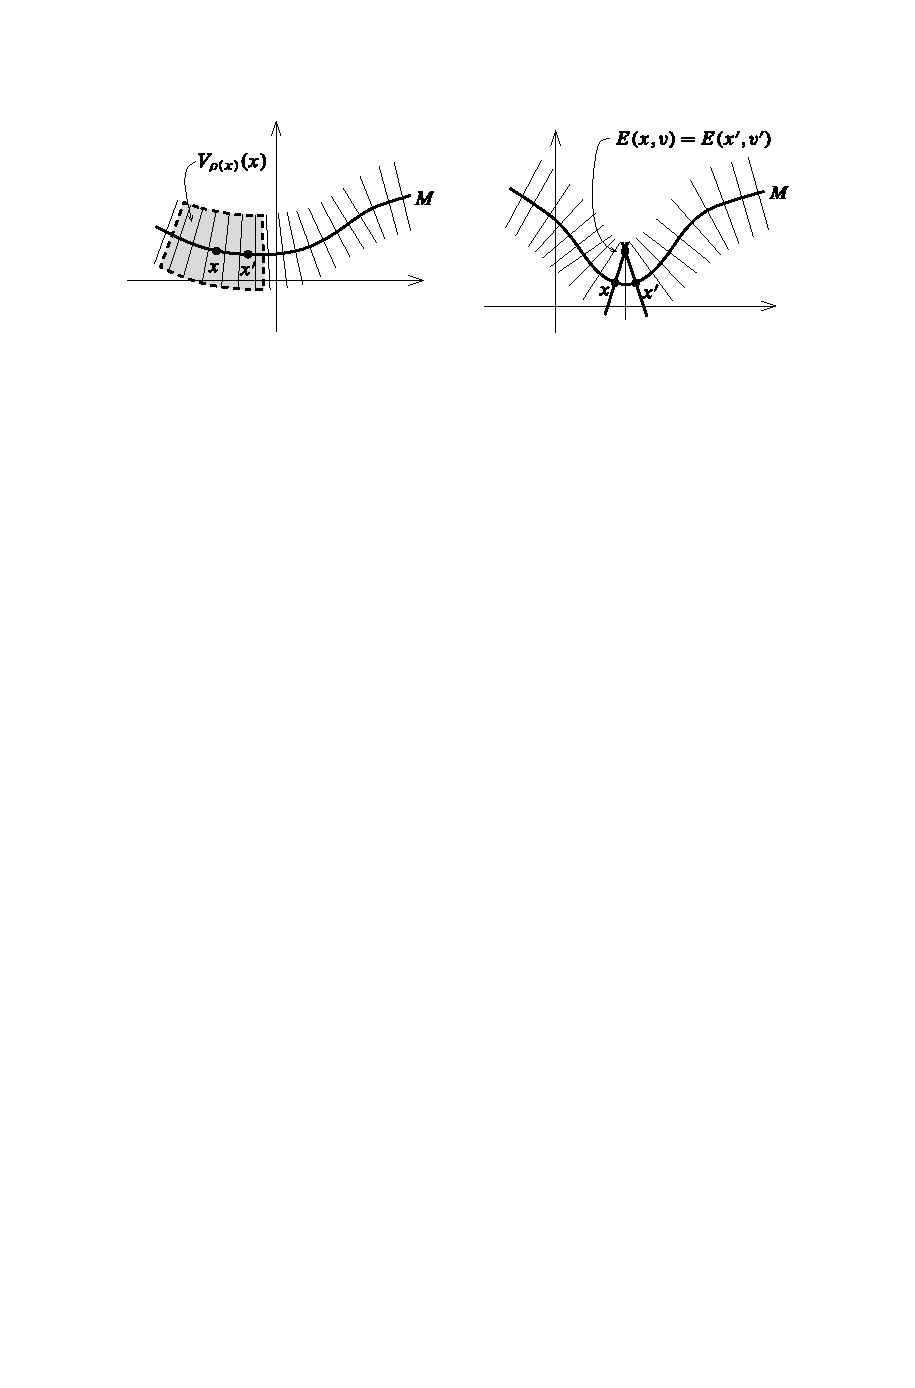
\includegraphics{pictures/tubular}
\caption{Continuity of $\rho$ and Injectivity of $E$.}
\end{figure}\par
To show it is continuous, let $x,x'\in P$ be arbitrary, and suppose first that $d_g(x,x')<\rho(x)$. Then by the triangle inequality, $V_\delta(x')$ is contained in 
$V_{\rho(x)}(x)$ for $\delta=\rho(x)-d_g(x,x')$, which implies that $\rho(x')\geq\rho(x)-d_g(x,x')$, or
\[\rho(x)-\rho(x')\leq d_g(x,x').\]

On the other hand, if $d_g(x,x')\geq\rho(x)$, then the inequality above holds for trivial reasons. Reversing the roles of $x$ and $x'$ yields an analogous inequality, 
which shows that $|\rho(x)-\rho(x')|\leq d_g(x,x')$, so $\rho$ is continuous.\par
Now let $V=\{(x,v)\in NP:|v|_g<\rho(x)/2\}$. We will show that $E$ is injective on $V$. Suppose that $(x,v)$ and $(x',v')$ are points in $V$ such that $E(x,v)=E(x',v')$. 
Assume without loss of generality that $\rho(x)\leq\rho(x')$. Because $\exp_x(v)=\exp_{x'}(v')$, there is an admissible curve from $x$ to $x'$ of length $|v|_g+|v'|_g$ 
(recall that the velocity of a geodesic is constant (Corollary~\ref{metric connection geodesic velocity constant})), and thus
\[d_g(x,x')\leq|v|_g+|v'|_g\leq\frac{1}{2}\rho(x)+\frac{1}{2}\rho(x')\leq\rho(x).\]
Therefore, both $(x,v)$ and $(x',v')$ are in $V_{\rho(x)}(x)$. Since $(x,v)$ and $(x',v')$ are then in $V_\delta(x)$ for some $\delta<\rho(x)$ and $E$ is injective on 
$V_\delta(x)$, this implies $(x,v)=(x',v')$.\par
The set $U=E(V)$ is open in $M$ because $E|_V$ is a local diffeomorphism and thus an open map. It follows that $E:V\to U$ is a smooth bijection and a local diffeomorphism, 
hence a diffeomorphism by Proposition~\ref{local diff prop}. Therefore, $U$ is a tubular neighborhood of $P$.\par
Finally, if $P$ is compact, then the continuous function $1/2\rho$ achieves a minimum value $\eps>0$ on $P$, so $U$ contains a uniform tubular neighborhood of radius $\eps$.
\end{proof}
\subsubsection{Fermi coordinates}
Now we will construct coordinates on a tubular neighborhood that are analogous to Riemannian normal coordinates around a point. Let $P$ be an embedded $k$-dimensional 
submanifold of a Riemannian $n$-manifold $(M,g)$, and let $U\sub M$ be a normal neighborhood of $P$, with $U=E(V)$ for some appropriate open subset $V\sub NP$.\par
Let $(W_0,\psi)$ be a smooth coordinate chart for $P$, and let $(E_1,\dots,E_{n-k})$ be a local orthonormal frame for the normal bundle $NP$; by shrinking $W_0$ if necessary, we can assume that the coordinates and the local frame are defined on the same open subset $W_0\sub P$. Let $\widehat{W}_0=\psi(W_0)\sub\R^k$, and let $NP|_{W_0}$ be the portion of the normal bundle over $W_0$. The coordinate map and frame $(E_j)$ yield a diffeomorphism $B:\widehat{W}_0\times\R^{n-k}\to NP|_{W_0}$ 
defined by
\[B(x^1,\dots,x^k,v^1,\dots,v^{n-k})=(p,v^1E_1|_p+\cdots+v^{n-k}E_{n-k}|_p),\]
where $p=\psi^{-1}(x^1,\dots,x^k)$. Let $V_0=V\cap NP|_{W_0}\sub NP$ and $U_0=E(V_0)\sub M$, and define a smooth coordinate map $\varphi:U_0\to\R^n$ by $\varphi=B^{-1}\circ(E|_{V_0})^{-1}$:
\[\begin{tikzcd}
NP|_{W_0}\ar[r,"B^{-1}"]&\widehat{W}_0\times\R^{n-k}\sub\R^n\\
U_0\ar[u,"(E|_{V_0})^{-1}"]\ar[ru,"\varphi"]
\end{tikzcd}\]
The coordinate map can also be written
\[\varphi:(p,v^1E_1|_p+\cdots+v^{n-k}E_{n-k}|_p)\mapsto(x^1(p),\dots,x^k(p),v^1,\dots,v^{n-k}).\]
Coordinates of this form are called \textbf{Fermi coordinates}. Here is the analogue of Proposition~\ref{Riemann normal coordinate prop} for Fermi coordinates.
\begin{proposition}[\textbf{Properties of Fermi Coordinates}]\label{Riemann Fermi coordinate prop}
Let $P$ be an embedded $k$-dimensional submanifold of a Riemannian $n$-manifold $(M,g)$, let $U$ be a normal neighborhood of $P$ in $M$, and let $(x^1,\dots,x^k,v^1,\dots,v^{n-k})$ 
be Fermi coordinates on an open subset $U_0\sub U$. For convenience, we also write $x^{k+j}=v^j$ for $j=1,\dots,n-k$.
\begin{itemize}
\item[(a)] $P\cap U_0$ is the set of points where $x^{k+1}=\cdots=x^n=0$.
\item[(b)] At each point $p\in P\cap U_0$, the metric components satisfy the following:
\[g_{ij}=g_{ji}=\begin{cases}
0,&1\leq i\leq k\text{ and }k+1\leq j\leq n;\\
\delta_{ij},&k+1\leq i,j\leq n.
\end{cases}\]
\item[(c)] For every $p\in P\cap U_0$ and $v=v^1E_1|_p+\cdots+v^{n-k}E_{n-k}|_p\in N_pP$, the geodesic $\gamma_v$ starting at $p$ with initial velocity $v$ is the curve 
with coordinate expression 
\[\gamma_v(t)=(x^1(p),\dots,x^k(p),tv^1,\dots,tv^{n-k}).\]
\item[(d)] At each $p\in P\cap U_0$, the Christoffel symbols in these coordinates satisfy $\Gamma_{ij}^k=0$, provided $k+1\leq i,j\leq n$.
\item[(e)] At each $p\in P\cap U_0$, the partial derivatives $\partial_ig_{jk}(p)$ vanish for $k+1\leq i,j,k\leq n$. 
\end{itemize}
\end{proposition}
\begin{proof}
Part (a) and (b) follow directly from the definition of Fermi coordinates, and (c) follows from Proposition~\ref{Riemann exp prop}(b).\par
To prove (d), let $v=v^iE_i|_p\in N_pP$ be arbitrary. The geodesic equation $(\ref{connection geodesic equation})$ for $\gamma_v(t)=(tv^1,\dots,tv^n)$ simplifies to
\[\Gamma_{ij}^k(x^1(p),\dots,x^k(p),tv^1,\dots,tv^{n-k})v^iv^j=0.\]
Evaluating this expression at $t=0$ shows that $\Gamma_{ij}^k(p)v^iv^j=0$ for every index $k$ and every vector $v$. In particular, with $v=\partial_a$ for some fixed 
$a$, this shows that $\Gamma_{aa}^k=0$ for each $a$ and $k$ (no summation). Substituting $v=\partial_a+\partial_b$ and $v=\partial_a-\partial_b$ for any fixed pair of 
indices $a$ and $b$ and subtracting, we conclude also that $\Gamma_{ab}^k$ at $p$ for all $a,b,k$. Finally, (e) follows from (d) together with 
$(\ref{metric connections char-1})$ in the case $E_k=\partial_k$.
\end{proof}
\subsection{Geodesics of the model spaces}
\subsubsection{Euclidean Space}
On $\R^n$ with the Euclidean metric, Proposition~\ref{Euclidean tangential connection symmetric} shows that the Levi-Civita connection is the Euclidean connection. 
Therefore, as one would expect, constant coefficient vector fields are parallel, and the Euclidean geodesics are straight lines with constant-speed parametrizations. 
Every Euclidean space is geodesically complete.
\subsubsection{Spheres}
Because the round metric on the sphere $S^n(R)$ is induced by the Euclidean metric on $\R^{n+1}$, it is easy to determine the geodesics on a sphere using 
Corollary~\ref{Euclidean geodesic submani}. Define a great circle on $S^n(R)$ to be any subset of the form $S^n(R)\cap\Pi$, where $\Pi\sub\R^{n+1}$ is a 
$2$-dimensional linear subspace.
\begin{proposition}
A nonconstant curve on $S^n(R)$ is a maximal geodesic if and only if it is a periodic constant-speed curve whose image is a great circle. Thus every sphere is geodesically complete.
\end{proposition}
\begin{proof}
Let $p\in S^n(R)$ be arbitrary. Because $f(x)=|x|^2$ is a defining function for $S^n(R)$, a vector $v\in T_p\R^{n+1}$ is tangent to $S^n(R)$ if and only if $df_p(v)=2\langle v,p\rangle=0$, 
where we think of $v$ as a vector by means of the usual identification of $\R^{n+1}$ with $T_p\R^{n+1}$. Thus $T_pS^n(R)$ is exactly the set of vectors orthogonal to $p$.\par
Suppose $v$ is an arbitrary nonzero vector in $T_pS^n(R)$. Let $a=|v|/R$ and $\hat{v}=v/a$ (so $\hat{v}=R$), and consider the smooth curve 
$\gamma:\R\to\R^{n+1}$ given by
\[\gamma(t)=(\cos at)p+(\sin at)\hat{v}.\]
By direct computation, $|\gamma(t)|^2=R^2$, so $\gamma(t)\in S^n(R)$ for all $t$. Moreover
\[\gamma'(t)=-a(\sin at)p+a(\cos at)\hat{v},\quad \gamma''(t)=-a^2(\cos at)p-a^2(\sin at)\hat{v}.\]
Because $\gamma''(t)$ is proportional to $\gamma(t)$ (thinking of both as vectors in $\R^{n+1}$), it follows that $\gamma''(t)$ is $\widebar{g}$-orthogonal to $T_pS^n(R)$, 
so $\gamma$ is a geodesic in $S^n(R)$ by Corollary~\ref{Euclidean geodesic submani}. Since $\gamma(0)=p$ and $\gamma(0)=a\hat{v}=v$, it follows that 
$\gamma=\gamma_v$.\par
Each $\gamma_v$ is periodic of period $2\pi/a$, and has constant speed by Corollary~\ref{metric connection geodesic velocity constant} (or by direct computation). The 
image of $\gamma_v$ is the great circle formed by the intersection of $S^n(R)$ with the linear subspace spanned by $\{p,\hat{v}\}$.\par
Conversely, suppose that $C$ is a great circle formed by intersecting $S^n(R)$ with a two dimensional subspace $\Pi$, and let $\{v,w\}$ be an orthonormal basis for $\Pi$. 
Then $C$ is the image of the geodesic with initial point $p=Rw$ and initial velocity $v$.
\end{proof}
\subsubsection{Hyperbolic spaces}
The geodesics of hyperbolic spaces can be determined by an analogous procedure
using the hyperboloid model.
\begin{proposition}
A nonconstant curve in a hyperbolic space is a maximal geodesic if and only if it is a constant-speed embedding of $\R$ whose image is one of the following:
\begin{itemize}
\item[(a)] Hyperboloid Model: The intersection of $\H^n(R)$ with a $2$-dimensional linear subspace of $\R^{n,1}$, called a \textbf{great hyperbola}.
\item[(b)] Beltrami-Klein: The interior of a line segment whose endpoints both lie on $\partial\K^n(R)$.
\item[(c)] Ball Model: The interior of a diameter of $\B^n(R)$, or the intersection of $\B^n(R)$ with a Euclidean circle that intersects $\partial\B^n(R)$ orthogonally.
\item[(d)] Half-Space Model: The intersection of $\mathbb{U}^n(R)$ with one of the following: a line parallel to the $y$-axis or a Euclidean circle with center on 
$\partial\mathbb{U}^n(R)$.
\end{itemize}
Every hyperbolic space is geodesically complete.
\end{proposition}
\begin{proof}
We begin with the hyperboloid model, for which the proof is formally quite similar to what we just did for the sphere. Since the Riemannian connection on $\H^n(R)$ is equal to the tangential connection by Proposition~\ref{Levi-Civita Euclidean}, it follows from Corollary~\ref{Euclidean geodesic submani} that a smooth curve $\gamma:I\to\H^n(R)$ is a geodesic if and only if its acceleration $\gamma''(t)$ is everywhere $\widebar{q}$-orthogonal to $T_{\gamma(t)}\H^n(R)$ (where $\widebar{q}=\widebar{q}^{n,1}$ is the Minkowski metric)\par
Let $p\in\H^n(R)$ be arbitrary. Note that $f(x)=\widebar{q}(x,x)$ is a defining function for $\H^n(R)$, and $(\ref{Hyperbolic space metric-1})$ shows that the gradient of $f$ at $p$ is equal to $2p$ (where we regard $p$ as a vector in $T_p\R^{n,1}$ as before). It follows that a vector $v\in T_p\R^{n,1}$ is tangent to $\H^n(R)$ if and only if $\widebar{q}(p,v)=0$. Let $v\in T_p\H^n(R)$ be an arbitrary nonzero vector. Put $a=|v|_{\widebar{q}}/R=\widebar{q}(v,v)^{1/2}/R$ and $\hat{v}=v/a$, and define $\gamma:\R\to\R^{n,1}$ by
\[\gamma(t)=(\cosh at)p+(\sinh at)\hat{v}.\]
Direct computation shows that $\gamma$ takes its values in $\H^n(R)$ and that its acceleration vector is everywhere proportional to $\gamma(t)$. Thus $\gamma''(t)$ is $\widebar{q}$-orthogonal to $T_{\gamma(t)}\H^n(R)$, so $\gamma$ is a geodesic in $\H^n(R)$ and therefore has constant speed. Because it satisfies the initial conditions $\gamma(0)=p$ and $\gamma'(t)=a\hat{v}=v$, it is equal to $\gamma_v$. Note that $\gamma_v$ is a smooth embedding of $\R$ into $H^n(R)$ whose image is the great hyperbola formed by the intersection between $\H^n(R)$ and the plane spanned by $\{p,\hat{v}\}$.\par
Conversely, suppose $\Pi$ is any $2$-dimensional linear subspace of $\R^{n,1}$ that has nontrivial intersection with $\H^n(R)$. Choose $p\in\Pi\cap\H^n(R)$, and let $v$ be another nonzero vector in $\Pi$ that is $\widebar{q}$-orthogonal to $p$, which implies $v\in T_p\H^n(R)$. Using the computation above, we see that the image of the geodesic $\gamma_v$ is the great hyperbola formed by the intersection of $\Pi$ with $\H^n(R)$.\par
Before considering the other three models, note that since maximal geodesics in $\H^n(R)$ are constant-speed embeddings of $\R$, it follows from naturality that maximal geodesics in each of the other models are also constant-speed embeddings of $\R$. Thus each model is geodesically complete, and to determine the geodesics in the other models we need only determine their images.\par
Consider the Beltrami–Klein model. Recall the isometry $c:\H^n(R)\to\K^n(R)$ given by $c(\xi,\tau)=R\xi/\tau$ (see (\ref{Hyperbolic central proj})). The image of a maximal geodesic in $\H^n(R)$ is a great hyperbola, which is the set of points $(\xi,\tau)\in\H^n(R)$ that solve a system of $n-1$ independent linear equations. Simple algebra shows that $(\xi,\tau)$ satisfies a linear equation $\alpha_i\xi^i+\beta\tau=0$ if and only if $w=c(\xi,\tau)=R\xi/\tau$ satisfies the affine equation $\alpha_i\xi^i=-\beta R$. Thus $c$ maps each great hyperbola onto the intersection of $\K^n(R)$ with an affine subspace of $\R^n$, and since it is the image of a smooth curve, it must be the intersection of $\K^n(R)$ with a straight line.\par
Next consider the Poincar\'e ball model. First consider the $2$-dimensional case, and recall the inverse hyperbolic stereographic projection $\pi^{-1}:\B^2(R)\to\H^2(R)$ constructed in Theorem~\ref{Hyperbolic space}:
\[\pi^{-1}(u)=(\xi,\tau)=\Big(\frac{2R^2u}{R^2-|u|^2},R\frac{R^2+|u|^2}{R^2-|u|^2}\Big).\]
In this case, a great hyperbola is the set of points on $\H^2(R)$ that satisfy a single linear equation $\alpha_i\xi^i+\beta\tau=0$. In the special case $\beta=0$, this hyperbola is mapped by $\pi$ to a straight line segment through the origin, as can easily be seen from the geometric definition of $\pi$. If $\beta\neq 0$, we can assume (after multiplying through by a constant if necessary) that $\beta=-1$, and write the linear equation as $\tau=\alpha_i\xi^i=\alpha\cdot\xi$ (where the dot represents the Euclidean dot product between elements of $\R^2$). Under $\pi^{-1}$, this pulls back to the equation
\[R\frac{R^2+|u|^2}{R^2-|u|^2}=\frac{2R^2\alpha\cdot u}{R^2-|u|^2}\]
on the disk, which simplifies to
\[|u|^2-2R\alpha\cdot u+R^2=0.\]
Completing the square, we can write this as
\begin{align}\label{Hyperbolic space geodesic-1}
|u-R\alpha|^2=R^2(|\alpha|^2-1)
\end{align}
If $|\alpha|^2\leq 1$, this locus is either empty or a point on $\partial\B^2(R)$, so it contains no points in $\B^2(R)$. Since we are assuming that it is the image of a maximal geodesic, we must therefore have $|\alpha|^2>1$. In that case, $(\ref{Hyperbolic space geodesic-1})$ is the equation of a circle with center $R$. and radius $R\sqrt{|\alpha|^2-1}$. At a point $u_0$ where the circle intersects $\partial\B^2(R)$, the three points $0$, $u_0$, and $R\alpha$ form a triangle with sides $|u_0|=R$, $|R\alpha|$, and $|u_0-R\alpha|$, which satisfy the Pythagorean identity by $(\ref{Hyperbolic space geodesic-1})$; therefore the circle meets $\partial\B^2(R)$ in a right angle.\par
In the higher-dimensional case, a geodesic on $\H^n(R)$ is determined by a $2$-plane. If the $2$-plane contains the point $(0,\dots,0,R)$, then the corresponding geodesic on $\B^n(R)$ is a line through the origin as before. Otherwise, we can use an orthogonal transformation in the $(\xi^1,\dots,\xi^n)$ variables (which preserves $\breve{g}_R$) to move this $2$-plane so that it lies in the $(\xi^1,\xi^2,\tau)$ subspace, and then we are in the same situation as in the $2$-dimensional case.\par
Finally, consider the upper half-space model. The $2$-dimensional case is easiest to analyze using complex notation. Recall the complex formula for the M\"obious transform $\kappa:\mathbb{U}^2(\R)\to\B^2(R)$ given in Theorem~\ref{Hyperbolic space}:
\[\kappa(z)=w=iR\frac{z-iR}{z+iR}.\]
Substituting this into equation (5.26) and writing $w=u+iv$ and $\alpha=a+ib$ in place of $u=(u^1,u^2)$, $\alpha=(\alpha^1,\alpha^2)$ we get
\[R^2\frac{|z-iR|^2}{|z+iR|^2}-iR^2\widebar{\alpha}\frac{z-iR}{z+iR}+iR^2\alpha\frac{\widebar{z}+iR}{\widebar{z}-iR}+R^2|\alpha|^2=R^2(|\alpha|^2-1).\]
Multiplying through by $(z+iR)(\widebar{z}-iR)/2R^2$ and simplifying yields
\[(1-b)|z|^2-2aRx+(b+1)R^2=0.\]
This is the equation of a circle with center on the $x$-axis, unless $b=1$, in which case the condition $|\alpha|^2>1$ forces $a\neq 0$, and then it is a straight line $x=$ constant. The other class of geodesics on the ball, line segments through the origin, can be handled similarly.\par
In the higher-dimensional case, suppose first that $\gamma:\R\to\mathbb{U}^n(R)$ is a maximal geodesic such that $\gamma(0)$ lies on the $y$-axis and $\gamma'(0)$ is in the span of $\{\partial/\partial x^1,\partial/\partial y\}$. From the explicit formula $(\ref{Hyperbolic space-1})$ for $\kappa$, it follows that $\kappa\circ\gamma(0)$ lies on the $v$-axis 
in the ball, and $(\kappa\circ\gamma)'(0)$ is in the span of $\{\partial/\partial u^1,\partial/\partial v\}$. The image of the geodesic $\kappa\circ\gamma$ is either part of a line through the origin or an arc of a circle perpendicular to $\partial\B^n(R)$, both of which are contained in the $(u^1,v)$-plane. By the argument in the preceding paragraph, it then follows that the image of $\gamma$ is contained in the $(x^1,y)$-plane and is either a vertical half-line or a semicircle centered on the $y=0$ hyperplane. For the general case, note that translations and orthogonal transformations in the $x$-variables preserve vertical half-lines and circles centered on the $y=0$ hyperplane in $\mathbb{U}^n(R)$, and they also preserve the metric $\breve{g}_R$. Given an arbitrary maximal geodesic $\gamma:\R\to\mathbb{U}^n(R)$, after applying an $x$-translation we may assume that $\gamma(0)$ lies on the $y$-axis, and after an orthogonal transformation in the $x$ variables, we may assume that $\gamma'(0)$ is in the span of $\{\partial/\partial x^1,\partial/\partial y\}$; then the argument above shows that the image of $\gamma$ is either a vertical half-line or a semicircle centered on the $y=0$ hyperplane.
\end{proof}
\subsection{Exercise}
\begin{exercise}\label{Riemann div as trace}
Suppose $(M,g)$ is a Riemannian manifold, and let $\div$ and $\nabla$ be the divergence and Laplace operators.
\begin{itemize}
\item[(a)] Show that for every vector field $X\in\X(M)$, $\div X$ can be written in terms of the total covariant derivative as $\div X=\tr(\nabla X)$, and that if 
$X=X_iE_i$ in terms of some local frame, then $\div X=X^i_{;i}$.
\item[(b)] Show that the Laplace operator acting on a smooth function $f$ can be expressed as 
\begin{align}\label{Riemann laplacian trace-1}
\Delta f=\tr_g(\nabla^2 f)
\end{align}
and in terms of any local frame,
\begin{align}\label{Riemann laplacian trace-2}
\Delta f=g^{ij}f_{;ij}={f_{;i}}^i.
\end{align}
\end{itemize}
\end{exercise}
\begin{proof}
Let $E_1,\dots,E_n$ be a local orthonormal frame and $dV_g$ the Riemannian volume form, then by definition and Proposition~\ref{Cartan magic}:
\[(\div X)dV_g=(d\circ i_X)(dV_g)=(d\circ i_X+i_X\circ d)(dV_g)=\mathfrak{L}_X(dV_g).\]
This then implies
\begin{align*}
\div X&=(\div X\,dV_g)(E_1,\dots,E_n)=(\mathfrak{L}_XdV_g)(E_1,\dots,E_n)\\
&=X(dV_g(E_1,\dots,E_n))-\sum_{i=1}^{n}dV_g(E_1,\dots,\nabla_XE_i,\dots,E_n)\\
&=-\sum_{i=1}^{n}\langle\mathfrak{L}_XE_i,E_i\rangle=\frac{1}{2}\sum_{i=1}^{n}(\mathfrak{L}_Xg)(E_i,E_i).
\end{align*}
Now we turn to $\tr(\nabla X)$. We have
\begin{align*}
\tr(\nabla X)&=\sum_{i=1}^{n}\langle(\nabla X)(E_i),E_i\rangle=\sum_{i=1}^{n}\langle\nabla_{E_i}X,E_i\rangle\\
&=\frac{1}{2}\sum_{i=1}^{n}\mathfrak{L}_Xg(E_i,E_i)+\frac{1}{2}\sum_{i=1}^{n}dX^{\flat}(E_i,E_i)=\frac{1}{2}\sum_{i=1}^{n}\mathfrak{L}_Xg(E_i,E_i),
\end{align*}
where we use Proposition~\ref{Riemann Levi-Civita Lie exterior} and that $dX^{\flat}$ is antisymmetric. This gives (a).\par
Now for part (b), we have 
\[\Delta f=\div(\grad f)=\tr(\nabla(\grad f))=\tr(\nabla (df)^{\sharp})=\tr((\nabla df)^{\sharp})=\tr_g(\nabla df)=\tr_g(\nabla^2 f).\]
The coordinate expression then follows.
\end{proof}
\section{Geodesics and distance}
Most of the results of this section do not apply to general pseudo-Riemannian metrics, at least not without substantial modification. For this reason, we restrict our focus here to the Riemannian case. Also, the theory of minimizing curves becomes considerably more complicated in the presence of a nonempty boundary; thus, unless otherwise stated, throughout this chapter we assume that $(M,g)$ is a Riemannian manifold without boundary. And because we will be using the Riemannian distance function, we assume for most results that $M$ is connected.
\subsection{Geodesics and minimizing curves}
Let $(M,g)$ be a Riemannian manifold. An admissible curve $\gamma$ in $M$ is said to be a minimizing curve if $L_g(\gamma)\leq L_g(\tilde{\gamma})$ for every admissible curve $\tilde{\gamma}$ with the same endpoints. When $M$ is connected, it follows from the definition of the Riemannian distance that $\gamma$ is minimizing if and only if $L_g(\gamma)$ is equal to the distance between its endpoints.\par
Our first goal is to show that all minimizing curves are geodesics. To do so, we will think of the length function $L_g$ as a functional on the set of all admissible curves in $M$ with fixed starting and ending points. Our project is to search for minima of this functional. It suffices to note that if $\gamma$ is a minimizing curve, and $\{\Gamma_s:s\in(-\eps,\eps)\}$ is a one-parameter family of admissible curves with the same endpoints such that $L_g(\Gamma_s)$ is a differentiable function of $s$ and $\Gamma_0=\gamma$, then by elementary calculus, the $s$-derivative of $L_g(\Gamma_s)$ must vanish at $s=0$ because $L_g(\gamma_s)$ attains a minimum there.
\subsubsection{Families of curves}
To make this rigorous, we introduce some more definitions. Let $(M,g)$ be a Riemannian manifold. Given intervals $I,J\sub\R$, a continuous map $\Gamma:J\times I\to M$ 
is called a \textbf{one parameter family of curves}. Such a family defines two collections of curves in $M$: the \textbf{main curves} $\Gamma_s(t)=\Gamma(s,t)$ defined 
for $t\in I$ by holding $s$ constant, and the \textbf{transverse curves} $\Gamma^t(s)=\Gamma(s,t)$ defined for $s\in I$ by holding $t$ constant. If such a family $\Gamma$ 
is smooth (or at least continuously differentiable), we denote the velocity vectors of the main and transverse curves by
\[\partial_t\Gamma(s,t)=(\Gamma_s)'(t)\in T_{\Gamma(s,t)}M,\quad\partial_s\Gamma(s,t)=(\Gamma^t)'(s)\in T_{\Gamma(s,t)}M.\]
Each of these is an example of a \textbf{vector field along $\bm{\Gamma}$}, which is a continuous map $V:I\times J\to TM$ such that $V(s,t)\in T_{\Gamma(s,t)}M$ for each $(s,t)$.
The families of curves that will interest us most are of the following type. A one-parameter family $\Gamma$ is called an admissible family of curves if 
\begin{itemize}
\item[(\rmnum{1})] its domain is of the form $J\times[a,b]$ for some open interval $J$.
\item[(\rmnum{2})] there is a partition $(a_0,\dots,a_k)$ of $[a,b]$ such that $\Gamma$ is smooth on each rectangle of the form $J\times[a_{i-1},a_i]$.
\item[(\rmnum{3})] $\Gamma_s(t)=\Gamma(s,t)$ is an admissible curve for each $s\in J$.
\end{itemize}
Every such partition is called an \textbf{admissible partition for the family}.\par
If $\gamma:[a,b]\to M$ is a given admissible curve, a \textbf{variation of $\bm{\gamma}$} is an admissible family of curves $\Gamma:J\times[a,b]\to M$ such that $J$ is 
an open interval containing $0$ and $\Gamma_0=\gamma$. It is called a proper variation if in addition, all of the main curves have the same starting and ending points: 
$\Gamma_s(a)=\gamma(a)$ and $\Gamma_s(b)=\gamma(b)$ for all $s\in J$.\par
In the case of an admissible family, the transverse curves are smooth on $J$ for each $t$, but the main curves are in general only piecewise regular. Thus the velocity 
vector fields $\partial_s\Gamma$ and $\partial_t\Gamma$ are smooth on each rectangle $J\times[a_{i-1},a_i]$, but not generally on the whole domain.
\begin{figure}[htbp]
\centering
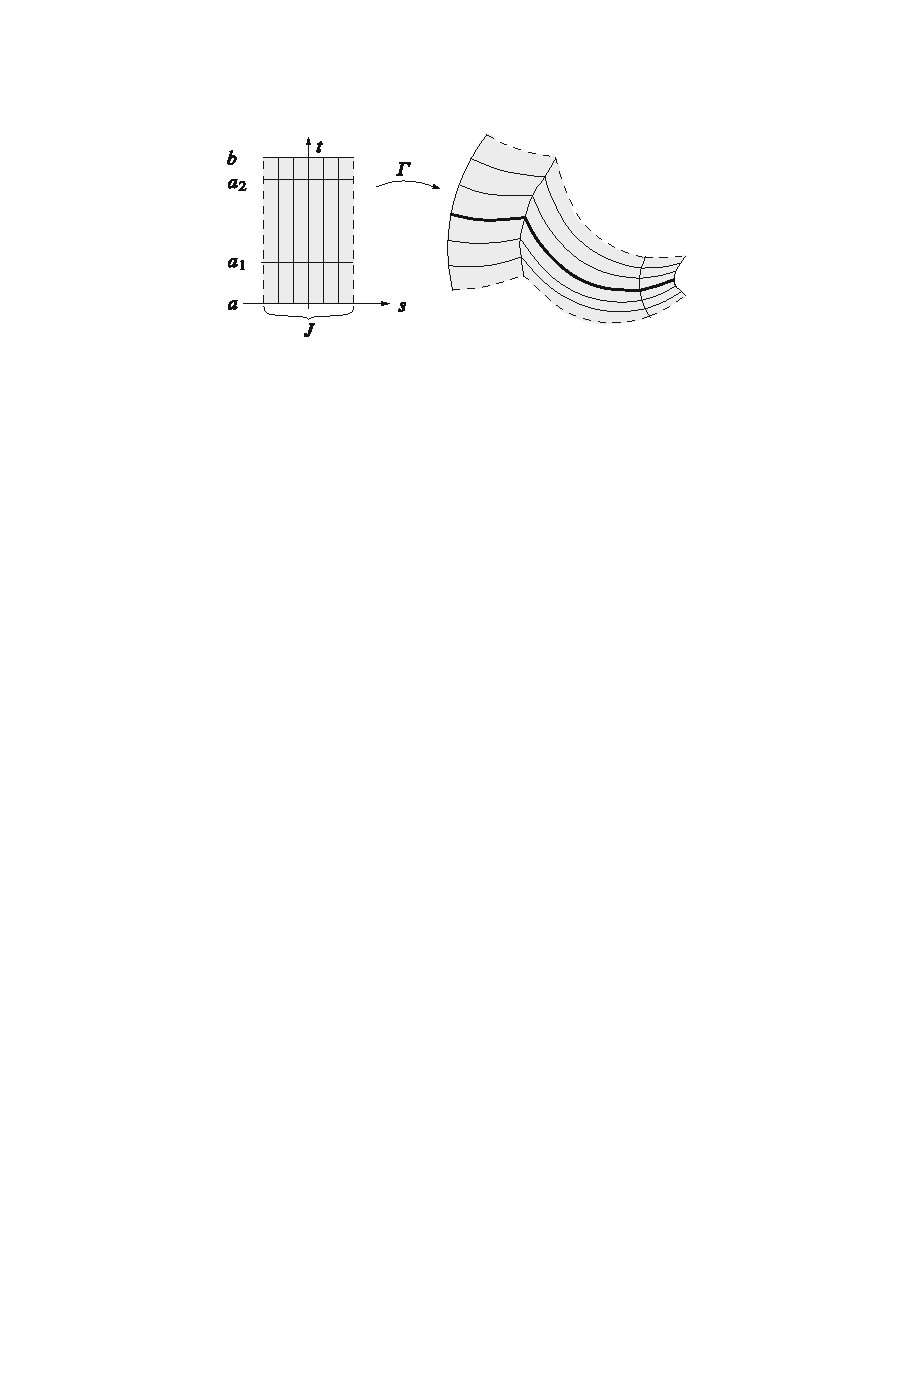
\includegraphics{pictures/admissible-family}
\caption{An admissible family.}
\end{figure}

We can say a bit more about $\partial_s\Gamma$, though. If $\Gamma$ is an admissible family, a \textbf{piecewise smooth vector field along $\bm{\Gamma}$} is a (continuous) 
vector field along $\gamma$ whose restriction to each rectangle $J\times[a_{i-1},a_i]$ is smooth for some admissible partition $(a_0,\dots,a_k)$ for $\Gamma$. In fact, 
$\partial_s\Gamma$ is always such a vector field. To see that it is continuous on the whole domain $J\times[a,b]$, note on the one hand that for each $i=1,\dots,k-1$, the 
values of $\partial_s\Gamma$ along the set $J\times\{a_i\}$ depend only on the values of $\Gamma$ on that set, since the derivative is taken only with respect to the 
$s$ variable; on the other hand,$\partial_s\Gamma$ is continuous (in fact smooth) on each subrectangle $J\times[a_{i-1},a_i]$ and $J\times[a_i,a_{i+1}]$, so the 
right-hand and left-hand limits at $t=a_i$ must be equal. Therefore $\partial_s\Gamma$ is always a piecewise smooth vector field along $\Gamma$. (However, 
$\partial_t\Gamma$ is typically not continuous at $t=a_i$.)\par
If $\Gamma$ is a variation of $\gamma$, the \textbf{variation field of $\bm{\Gamma}$} is the piecewise smooth vector field $V(t)=\partial_s\Gamma(0,t)$ along $\gamma$. 
We say that a vector field $V$ along $\gamma$ is \textbf{proper} if $V(a)=V(b)=0$; it follows easily from the definitions that the variation field of every proper 
variation is itself proper.
\begin{proposition}\label{Riemann variation field}
If $\gamma$ is an admissible curve and $V$ is a piecewise smooth vector field along $\gamma$, then $V$ is the variation field of some variation of $\gamma$. If $V$ is 
proper, the variation can be taken to be proper as well.
\end{proposition}
\begin{figure}[htbp]
\centering
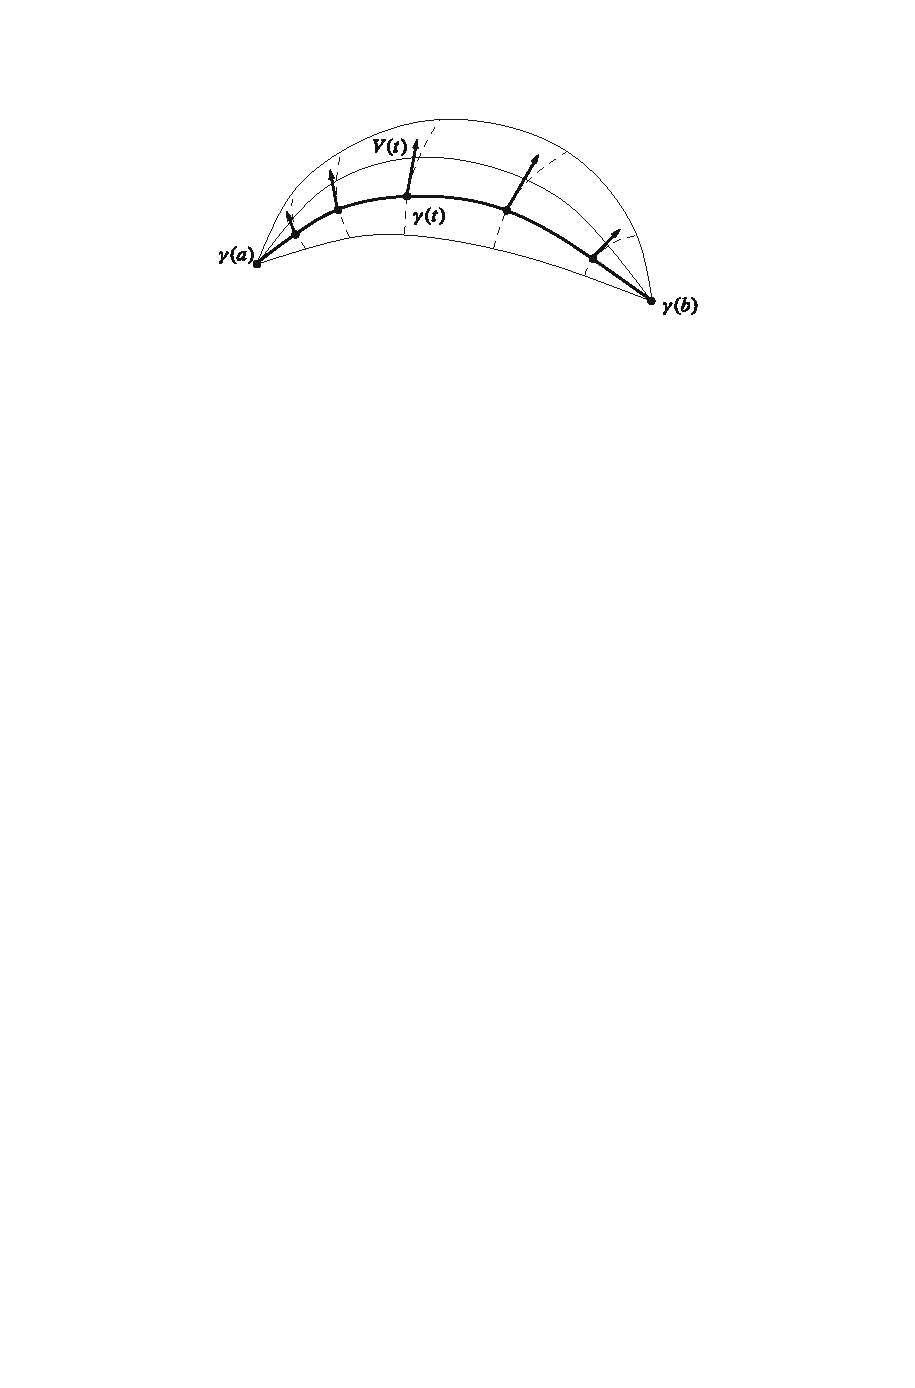
\includegraphics{pictures/variation-field}
\caption{Every vector field along $\gamma$ is a variation field.}
\end{figure}
\begin{proof}
Suppose $\gamma$ and $V$ satisfy the hypotheses, and set $\Gamma(s,t)=\exp_{\gamma(t)}(sV(t))$. By compactness of $[a,b]$, there is some positive $\eps$ such that $\Gamma$ 
is defined on $(-\eps,\eps)\times[a,b]$. By composition, $\Gamma$ is smooth on $(-\eps,\eps)\times[a_{i-1},a_i]$ for each subinterval $[a_{i-1},a_i]$ on which $V$ is 
smooth, and it is continuous on its whole domain. By the properties of the exponential map, the variation field of $\Gamma$ is $V$. Moreover, if $V(a)=0$ and $V(b)=0$, 
the definition gives $\Gamma(0,a)\equiv\gamma(a)$ and $\Gamma(0,b)\equiv\gamma(b)$, so $\Gamma$ is proper.
\end{proof}
If $V$ is a piecewise smooth vector field along $\Gamma$, we can compute the covariant derivative of $V$ either along the main curves (at points where $V$ is smooth) or 
along the transverse curves; the resulting vector fields along $\Gamma$ are denoted by $D_tV$ and $D_sV$ respectively. A key ingredient in the proof that minimizing 
curves are geodesics is the symmetry of the Levi-Civita connection. It enters into our proofs in the form of the following lemma. 
\begin{lemma}[\textbf{Symmetry Lemma}]\label{Riemann symmetry lemma}
Let $\Gamma:J\times[a,b]\to M$ be an admissible family of curves in a Riemannian manifold. On every rectangle $J\times[a_{i-1},a_i]$ where $\Gamma$ is smooth,
\[D_s\partial_t\Gamma=D_t\partial_s\Gamma.\]
\end{lemma}
\begin{proof}
This is a local question, so we may compute in local coordinates $(x^i)$ around a point $\Gamma(s_0,t_0)$. Writing the components of $\Gamma$ as 
$\Gamma(s,t)=(x^1(s,t),\dots,x^n(s,t))$, we have
\[\partial_t\Gamma=\frac{\partial x^k}{\partial t}\partial_k,\quad \partial_s\Gamma=\frac{\partial x^k}{\partial s}\partial_k.\]
Then, using the coordinate formula $(\ref{connection derivative curve-1})$ for covariant derivatives along curves, we obtain
\[D_s\partial_t\Gamma=\Big(\frac{\partial^2x^k}{\partial s\partial t}+\frac{\partial x^i}{\partial s}\frac{\partial x^j}{\partial t}\Gamma_{ij}^k\Big)\partial_k,\quad D_t\partial_s\Gamma=\Big(\frac{\partial^2x^k}{\partial t\partial s}+\frac{\partial x^i}{\partial t}\frac{\partial x^j}{\partial s}\Gamma_{ij}^k\Big)\partial_k.\]
Reversing the roles of $i$ and $j$ in the second line above and using the symmetry condition $\Gamma_{ij}^k=\Gamma_{ji}^k$, we conclude that these two expressions are 
equal.
\end{proof}
\subsubsection{Minimizing curves are geodesics}
We can now compute an expression for the derivative of the length functional along a variation of a curve. Traditionally, the derivative of a functional on a space of 
maps is called its \textbf{first variation}.
\begin{theorem}[\textbf{First Variation Formula}]\label{Riemann geodesic first variation}
Let $(M,g)$ be a Riemannian manifold. Suppose $\gamma:[a,b]\to M$ is a unit-speed admissible curve, $\Gamma:J\times[a,b]\to M$ is a variation of $\gamma$, and $V$ is its 
variation field. Then $L_g(\Gamma_s)$ is a smooth function of $s$, and
\begin{align}\label{geodesic first variation-1}
\frac{d}{ds}\Big|_{s=0}L_g(\Gamma_s)=-\int_{a}^{b}\langle V,D_t\gamma'\rangle dt-\sum_{i=1}^{k-1}\langle V(a_i),\Delta_i\gamma'\rangle+\langle V,\gamma'\rangle\Big|_{a}^{b}.
\end{align}
where $(a_0,\dots,a_k)$ is an admissible partition for $V$, and for each $i=1,\dots,k-1$, $\Delta_i\gamma'=\gamma'(a_i^+)-\gamma'(a_i^-)$ is the "jump" in the velocity vector 
field $\gamma'$ at $a_i$. In particular, if $\Gamma$ is a proper variation, then
\begin{align}\label{geodesic first variation-2}
\frac{d}{ds}\Big|_{s=0}L_g(\Gamma_s)=-\int_{a}^{b}\langle V,D_t\gamma'\rangle dt-\sum_{i=1}^{k-1}\langle V(a_i),\Delta_i\gamma'\rangle.
\end{align}
\end{theorem}
\begin{proof}
On every rectangle $J\times[a_{i-1},a_i]$ where $\Gamma$ is smooth, since the integrand in $L_g(\Gamma_s)$ is smooth and the domain of integration is compact, we can 
differentiate under the integral sign as many times as we wish. Because $L_g(\Gamma_s)$ is a finite sum of such integrals, it follows that it is a smooth function of $s$.\par
Differentiating on the interval $[a_{i-1},a_i]$ yields
\begin{align*}
\frac{d}{ds}L_g(\Gamma_s|_{[a_{i-1},a_i]})&=\int_{a_{i-1}}^{a_i}\frac{\partial}{\partial s}|\partial_t\Gamma_s|dt\\
&=\int_{a_{i-1}}^{a_i}\frac{1}{2|\partial_t\Gamma|}(\langle D_s\partial_t\Gamma,\partial_t\Gamma\rangle+\langle\partial_t\Gamma,D_s\partial_t\Gamma\rangle)dt\\
&=\int_{a_{i-1}}^{a_i}\frac{\langle D_s\partial_t\Gamma,\partial_t\Gamma\rangle}{|\partial_t\Gamma|}dt\\
&=\int_{a_{i-1}}^{a_i}\frac{\langle D_t\partial_s\Gamma,\partial_t\Gamma\rangle}{|\partial_t\Gamma|}dt
\end{align*}
where we have used the symmetry lemma in the last line. Setting $s=0$ and noting that $\partial_s\Gamma(0,t)=V(t)$ and $\partial_t\Gamma(0,t)=\gamma'(t)$ (which has length $1$), 
we get
\begin{align*}
\frac{d}{ds}\Big|_{s=0}L_g(\Gamma_s|_{[a_{i-1},a_i]})&=\int_{a_{i-1}}^{a_i}\langle D_tV,\gamma'\rangle dt=\int_{a_{i-1}}^{a_i}\Big(\frac{d}{dt}\langle V,\gamma'\rangle-\langle V,D_t\gamma'\rangle\Big)dt\\
&=\langle V(a_i),\gamma'(a_i^-)\rangle-\langle V(a_{i-1}),\gamma'(a_{i-1}^+)\rangle-\int_{a_{i-1}}^{a_i}\langle V,D_t\gamma'\rangle dt.
\end{align*}
Finally, summing over $i$, we obtain $(\ref{geodesic first variation-1})$.
\end{proof}
Because every admissible curve has a unit-speed parametrization and length is independent of parametrization, the requirement in the above proposition that $\gamma$ be of 
unit speed is not a real restriction, but rather just a computational convenience.
\begin{theorem}\label{Riemann minimizing is geodesic}
In a Riemannian manifold, every minimizing curve is a geodesic when it is given a unit-speed parametrization.
\end{theorem}
\begin{proof}
Suppose $\gamma:[a,b]\to M$ is minimizing and of unit speed, and $(a_0,\dots,a_k)$ is an admissible partition for $\gamma$. If $\Gamma$ is any proper variation of $\gamma$, 
then $L_g(\Gamma_s)$ is a smooth function of $s$ that achieves its minimum at $s=0$, so it follows from elementary calculus that $d(L_g(\Gamma_s))/ds=0$ when $s=0$. Since 
every proper vector field along $\gamma$ is the variation field of some proper variation, the right-hand side of $(\ref{geodesic first variation-2})$ must vanish for 
every such $V$.\par
First we show that $D_t\gamma'=0$ on each subinterval $[a_{i-1},a_i]$, so $\gamma$ is a "broken geodesic". Choose one such interval, and let $\varphi\in C^{\infty}(\R)$ be 
a bump function such that $\varphi>0$ on $(a_{i-1},a_i)$ and $\varphi=0$ elsewhere. Then $(\ref{geodesic first variation-2})$ with $V=\varphi D_t\gamma'$ becomes
\[0=-\int_{a_{i-1}}^{a_i}\varphi|D_t\gamma'|^2dt.\]
Since the integrand is nonnegative and $\varphi>0$ on $(a_{i-1},a_i)$, this shows that $D_t\gamma'=0$ on each such subinterval.\par
Next we need to show that $\Delta_i\gamma'=0$ for each $i$ between $0$ and $k$, which is to say that $\gamma$ has no corners. For each such $i$, we can use a bump 
function in a coordinate chart to construct a piecewise smooth vector field $V$ along $\gamma$ such that $V(a_i)=\Delta_i\gamma'$ and $V(a_{j})=0$ for $j\neq i$. Then 
$(\ref{geodesic first variation-2})$ reduces to $-|\Delta_i\gamma'|^2=0$, so $\Delta_i\gamma'=0$ for each $i$.\par
Finally, since the two one-sided velocity vectors of $\gamma$ match up at each $a_i$, it follows from uniqueness of geodesics that $\gamma|_{[a_{i},a_{i+1}]}$ is the 
continuation of the geodesic $\gamma|_{[a_{i-1},a_i]}$, and therefore $\gamma$ is smooth.
\end{proof}
The first variation formula actually tells us a bit more than is claimed in Theorem~\ref{Riemann minimizing is geodesic}. In proving that $\gamma$ is a geodesic, we did not use the full strength of 
the assumption that the length of $\Gamma_s$ takes a minimum when $s=0$; we only used the fact that its derivative is zero. We say that an admissible curve $\gamma$ is 
a critical point of $L_g$ if for every proper variation $\Gamma_s$ of $\gamma$, the derivative of $L_g(\Gamma_s)$ with respect to $s$ is zero at $s=0$. Therefore we can 
strengthen Theorem~\ref{Riemann minimizing is geodesic} in the following way.
\begin{corollary}\label{Riemann critical of L_g iff geodesic}
A unit-speed admissible curve $\gamma$ is a critical point for $L_g$ if and only if it is a geodesic.
\end{corollary}
The geodesic equation $D_t\gamma'=0$ thus characterizes the critical points of the length functional. In general, the equation that characterizes critical points of a 
functional on a space of maps is called the variational equation or the \textbf{Euler-Lagrange equation} of the functional.
\subsubsection{Geodesics are locally minimizing}
Next we turn to the converse of Theorem~\ref{Riemann minimizing is geodesic}. It is easy to see that the literal converse is not true, because not every geodesic segment is 
minimizing. For example, every geodesic segment on $S^n$ that goes more than halfway around the sphere is not minimizing, because the other portion of the same great 
circle is a shorter curve segment between the same two points. For that reason, we concentrate initially on local minimization properties of geodesics.\par
As usual, let $(M,g)$ be a Riemannian manifold. A regular (or piecewise regular) curve $\gamma:I\to M$ is said to be \textbf{locally minimizing} if every $t_0\in I$ has a 
neighborhood $I_0\sub I$ such that whenever $a,b\in I_0$ with $a<b$, the restriction of $\gamma$ to $[a,b]$ is minimizing.
\begin{lemma}\label{Riemann minimizing is local minimizing}
Every minimizing admissible curve segment is locally minimizing.
\end{lemma}
\begin{proof}
Let $\gamma:I\to M$ be a minimizing admissible curve, then for any $a,b\in I$ the restriction $\gamma|_{[a,b]}$ is also minimizing, since otherwise we can replace this 
segment by a minimizing curve, which contradictc the fact that $\gamma$ is a minimizing curve.
\end{proof}
Our goal is to show that geodesics are locally minimizing. The proof will be based on a careful analysis of the geodesic equation in Riemannian normal coordinates. If $\eps$ is a positive number such that $\exp_p$ is a diffeomorphism from the ball $B_\eps(0)\sub T_pM$ to its image (where the radius of the ball is measured with respect to the norm defined by $g_p$), then the image set $\exp_p(B_\eps(0))$ is a normal neighborhood of $p$, called a \textbf{geodesic ball in $\bm{M}$}, or sometimes an \textbf{open geodesic ball} for clarity. Also, if the closed ball $\widebar{B_{\eps}(0)}$ is contained in an open set $V\sub T_pM$ on which $\exp_p$ is a diffeomorphism onto its image, then $\exp_p(\widebar{B_\eps(0)})$ is called a \textbf{closed geodesic ball}, and $\exp_p(\partial B_\eps(0))$ is called a \textbf{geodesic sphere}. Given such a $V$, by compactness there exists $\eps'>\eps$ such that $B_{\eps'}(0)\sub V$, so every closed geodesic ball is contained in an open geodesic ball of larger radius. In Riemannian normal coordinates centered at $p$, the open and closed geodesic balls and geodesic spheres centered at $p$ are just the coordinate balls and spheres.\par
Suppose $U$ is a normal neighborhood of $p\in M$. Given any normal coordinates $(x^i)$ on $U$ centered at $p$, define the \textbf{radial distance function} $r:U\to\R$ by
\begin{align}\label{Riemann radial diatance def}
r(x)=\sqrt{(x^1)^2+\cdots+(x^n)^2}.
\end{align}
and the \textbf{radial vector field} on $U\setminus\{p\}$, denoted by $\partial_r$, by
\begin{align}\label{Riemann radial vector field def}
\frac{\partial}{\partial r}=\frac{x^i}{r}\frac{\partial}{\partial x^i}.
\end{align}
In Euclidean space, $r(x)$ is the distance to the origin, and $\partial_r$ is the unit vector field pointing radially outward from the origin. (The notation is suggested by the fact that $\partial_r$ is a coordinate derivative in polar or spherical coordinates.)
\begin{lemma}\label{Riemann radial distance smooth}
In every normal neighborhood $U$ of $p\in M$, the radial distance function and the radial vector field are well defined, independently of the choice of normal coordinates. Both $r$ and $\partial_r$ are smooth on $U\setminus\{p\}$, and $r^2$ is smooth on all of $U$.
\end{lemma}
\begin{proof}
Proposition~\ref{Riemann normal coordinate prop} shows that any two normal coordinate charts on $U$ are related by $\tilde{x}^i=A^i_jx^j$ for some orthogonal matrix $(A^i_j)$, and a straightforward computation shows that both $r$ and $\partial_r$ are invariant under such coordinate changes:
\[r(x)=|x|=|Ax|,\quad\frac{\partial}{\partial r}=\frac{\tilde{x}^i}{r}\frac{\partial}{\partial\tilde{x}^i}=\frac{A^i_jx^j}{r}\frac{\partial}{\partial\tilde{x}^i}=\frac{x^j}{r}\frac{\partial\tilde{x}^i}{\partial x^j}\frac{\partial}{\partial\tilde{x}^i}=\frac{x^j}{r}\frac{\partial}{\partial x^j}.\]
The smoothness statements follow directly from the coordinate formulas.
\end{proof}
The crux of the proof that geodesics are locally minimizing is the following deceptively simple geometric lemma.
\begin{theorem}[\textbf{The Gauss Lemma}]\label{Gauss lemma}
Let $(M,g)$ be a Riemannian manifold, let $U$ be a geodesic ball centered at $p\in M$, and let $\partial_r$ denote the radial vector field on $U\setminus\{p\}$. Then  $\partial_r$ is a unit vector field orthogonal to the geodesic spheres in $U\setminus\{p\}$.
\end{theorem}
\begin{proof}
We will work entirely in normal coordinates $(x^i)$ on $U$ centered at $p$, using the properties of normal coordinates described in Proposition~\ref{Riemann normal coordinate prop}. Let $q\in U\setminus\{p\}$ be arbitrary, with coordinate representation $(q_1,\dots,q_n)$. It follows that $\partial_r|_q$ has the coordinate representation
\[\frac{\partial}{\partial r}\Big|_{q}=\frac{q^i}{r(q)}\frac{\partial}{\partial x^i}\Big|_{q}.\]
Let $v=v^i\partial_i\in T_pM$ be the tangent vector at $p$ with components $v^i=q^i/r(q)$. By Proposition~\ref{Riemann normal coordinate prop}(c), the radial geodesic with initial velocity $v$ is given in these coordinates by
\[\gamma_v(t)=(tv^1,\dots,tv^n).\]
It satisfies $\gamma(0)=p$, $\gamma(r(q))=q$, and $\gamma'_v(r(q))=v^i\partial_i|_q=\partial_r|_q$. Because $g_p$ is equal to the Euclidean metric in these coordinates (Proposition~\ref{Riemann normal coordinate prop}(b)), we have
\[|\gamma'_v(0)|_g=|v|_g=\sqrt{(v^1)^2+\cdots+(v^n)^2}=\frac{1}{r(q)}\sqrt{(q^1)^2+\cdots+(q^n)^2}=1.\]
so $v$ is a unit vector, and thus $\gamma_v$ is a unit-speed geodesic. It follows that $\partial_r=\gamma'_v(b)$ is also a unit vector.\par
To prove that $\partial_r$ is orthogonal to the geodesic spheres, let $q$ and $v$ be as above, and let $\Sigma_{r(q)}$ be the geodesic sphere containing $q$. In these coordinates, $\Sigma_{r(q)}=\exp_p(\partial B_{r(q)}(0))$ is the set of points satisfying the equation $(x^1)^2+\cdots+(x^n)^2=r^2(q)$. Let $w\in T_qM$ be any vector tangent to $\Sigma_{r(q)}$ at $q$. We need to show that $\langle w,\partial_r|_q\rangle=0$.
\begin{figure}[htbp]
\centering
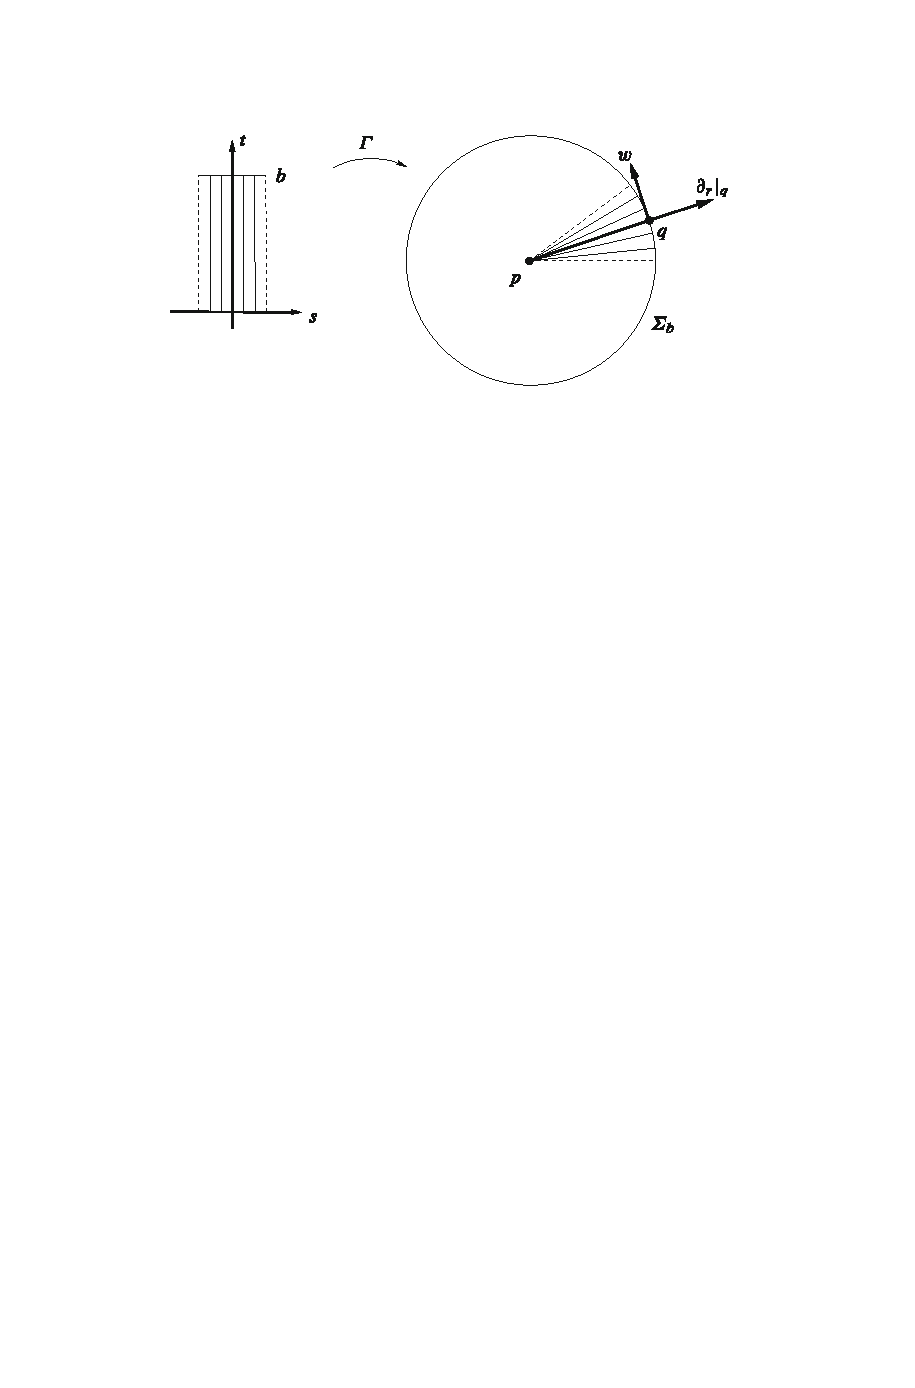
\includegraphics{pictures/Gauss-lemma}
\caption{Proof of the Gauss lemma.}
\end{figure}

Choose a smooth curve $\sigma:(-\eps,\eps)\to\Sigma_{r(q)}$ satisfying $\sigma(0)=q$ and $\sigma'(0)=w$, and write its coordinate representation in $(x^i)$-coordinates as $\sigma(s)=(\sigma^1(s),\dots,\sigma^n(s))$. The fact that $\sigma(s)$ lies in $\Sigma_{r(q)}$ for all $s$ means that 
\begin{align}\label{Gauss lemma-1}
(\sigma^1)^2+\cdots+(\sigma^n)^2=r^2(q).
\end{align}
Define a smooth map $\Gamma:(-\eps,\eps)\times[0,r(q)]\to M$ by
\[\Gamma(s,t)=\frac{t}{r(q)}\sigma(s).\]
For each $s\in(-\eps,\eps)$, $\Gamma_s$ is a geodesic by Proposition~\ref{Riemann normal coordinate prop}(c). Its initial velocity is 
\[\Gamma'_s(0)=\frac{\sigma(s)}{r(q)},\]
which is a unit vector by $(\ref{Gauss lemma-1})$ and the fact that $g_p$ is the Euclidean metric in coordinates; thus each $\Gamma_s$ is a unit-speed geodesic.\par
Note that $\Gamma(0,t)=\gamma_v(t)$, so it now follows from the definitions that
\[\partial_s\Gamma(0,0)=\frac{d}{ds}\Big|_{s=0}\Gamma_s(0)=0,\quad \partial_t\Gamma(0,0)=\frac{d}{dt}\Big|_{t=0}\gamma_v(t)=v;\]
\[\partial_s\Gamma(0,r(q))=\frac{d}{ds}\Big|_{s=0}\sigma(s)=w,\quad \partial_t\Gamma(0,r(q))=\frac{d}{dt}\Big|_{s=r(q)}\gamma_v(t)=\partial_r|_q.\]
Therefore $\langle\partial_s\Gamma,\partial_t\Gamma\rangle$ is zero when $(s,t)=(0,0)$ and equal to $\langle w,\partial_r|_q\rangle$ when $(s,t)=(0,r(q))$, so to prove the theorem it suffices to show that 
$\langle\partial_s\Gamma,\partial_t\Gamma\rangle$ is independent of $t$. We compute
\begin{equation}\label{Guass lemma-1}
\begin{aligned}
\frac{d}{dt}\langle\partial_s\Gamma,\partial_t\Gamma\rangle&=\langle D_t\partial_s\Gamma,\partial_t\Gamma\rangle+\langle\partial_s\Gamma,D_t\partial_t\Gamma\rangle\\
&=\langle D_t\partial_s\Gamma,\partial_t\Gamma\rangle=\langle D_s\partial_t\Gamma,\partial_t\Gamma\rangle\\
&=\frac{1}{2}\frac{\partial}{\partial s}|\partial_t\Gamma|^2=0.
\end{aligned}
\end{equation}
where we use the symmetry lemma and the fact that each $\Gamma_s$ is a unit-speed geodesic. This proves the theorem.
\end{proof}
\begin{corollary}\label{Riemann radial distance grad}
Let $U$ be a geodesic ball centered at $p\in M$, and let $r$ and $\partial_r$ be the radial distance and radial vector field. Then $\grad r=\partial r$ on $U\setminus\{p\}$.
\end{corollary}
\begin{proof}
By the result of Exercise~\ref{Riemann grad prop}, it suffices to show that $\partial_r$ is orthogonal to the level sets of $r$ and $\partial_r(r)\equiv|\partial_r|_g^2$. The first claim follows directly from the Gauss lemma, and the second from the fact that $\partial_r(r)=1$ by direct computation in normal coordinates, which in turn is equal to $|\partial_r|_g^2$ by the Gauss lemma.
\end{proof}
\begin{proposition}\label{Riemann geodesic ball radial is minimize}
Let $(M,g)$ be a Riemannian manifold. Suppose $p\in M$ and $q$ is contained in a geodesic ball around $p$. Then (up to reparametrization) the radial geodesic from $p$ 
to $q$ is the unique minimizing curve in $M$ from $p$ to $q$.
\end{proposition}
\begin{proof}
Choose $\eps>0$ such that $\exp_p(B_{\eps}(0))$ is a geodesic ball containing $q$. Let $\gamma:[0,c]\to M$ be the radial geodesic from $p$ to $q$ parametrized by arc length, and write $\gamma(t)=\exp_p(tv)$ for some unit vector $v\in T_pM$. Then $L_g(\gamma)=c$, since $\gamma$ has unit speed.
\begin{figure}[htbp]
\centering
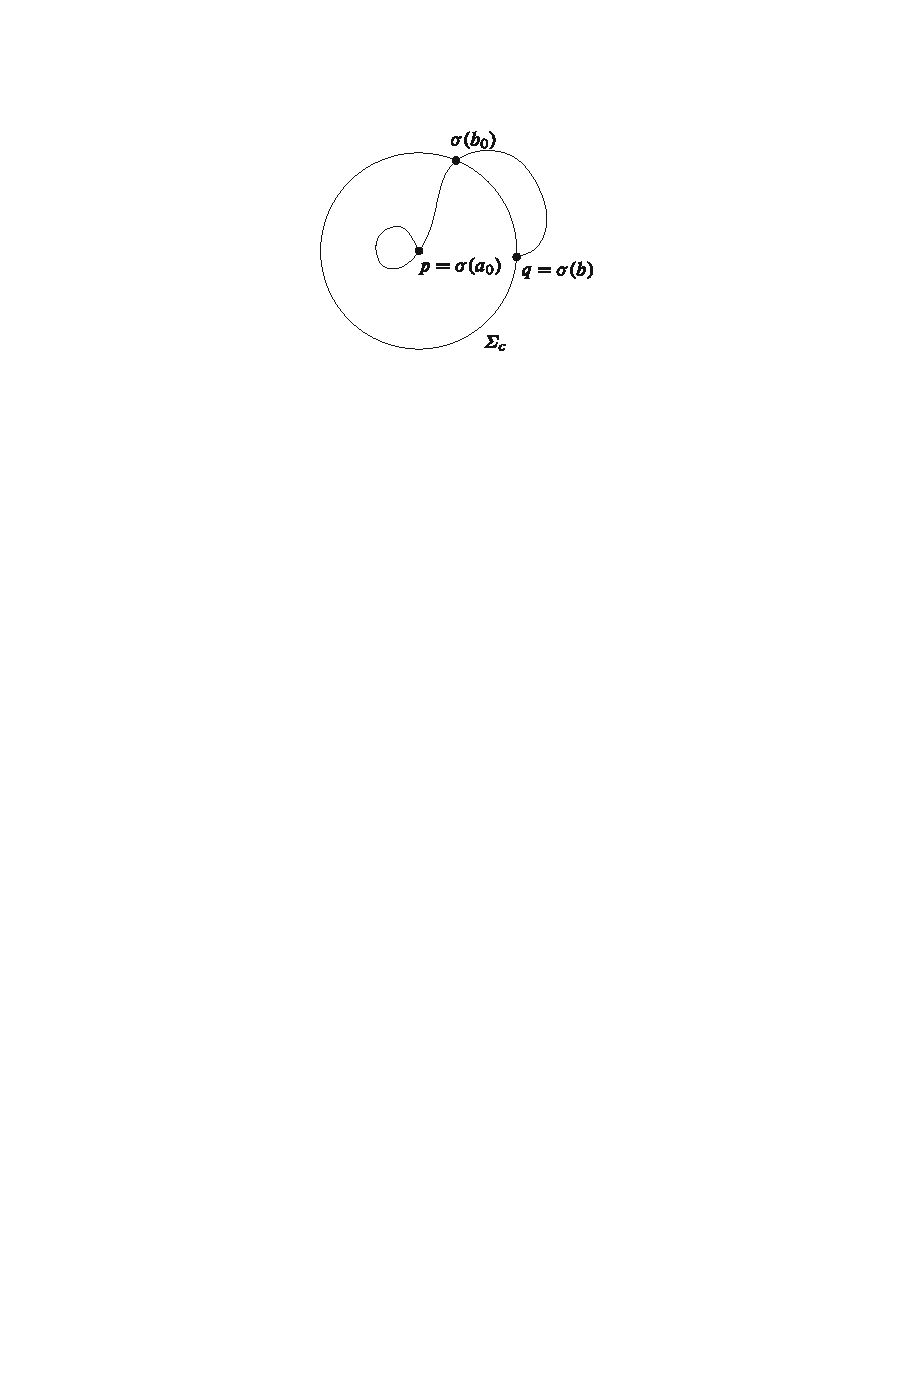
\includegraphics{pictures/radial-geodesic}
\caption{Radial geodesics are minimizing.}
\end{figure}

To show that $\gamma$ is minimizing, we need to show that every other admissible curve from $p$ to $q$ has length at least $c$. Let $\sigma:[0,b]\to M$ be an arbitrary 
admissible curve from $p$ to $q$, which we may assume to be parametrized by arc length as well. Let $a_0\in[0,b]$ denote the last time that $\sigma(t)=p$, and $b_0\in[0,b]$ the first time after $a_0$ that $\sigma(t)$ meets the geodesic sphere $\Sigma_c$ of radius $c$ around $p$. Then the composite function $r\circ\sigma$ is continuous on $[a_0,b_0]$ and piecewise smooth in $(a_0,b_0)$, so we can apply the fundamental theorem of calculus to conclude that
\begin{equation}\label{Riemann geodesic ball minimize-1}
\begin{aligned}
r(\sigma(b_0))-r(\sigma(a_0))&=\int_{a_0}^{b_0}\frac{d}{dt}r(\sigma(t))dt=\int_{a_0}^{b_0}\langle\grad r|_{\sigma(t)},\sigma'(t)\rangle dt\\
&\leq\int_{a_0}^{b_0}|\grad r|_{\sigma(t)}|\cdot|\sigma'(t)|dt\\
&=\int_{a_0}^{b_0}|\sigma'(t)|dt=L_g(\sigma|_{[a_0,b_0]}).
\end{aligned}
\end{equation}
Thus $L_g(\sigma)\geq r(\sigma(b_0))-r(\sigma(a_0))=c$, so $\gamma$ is minimizing.\par
Now suppose $L_g(\sigma)=c$. Then $b=c$, and $a_0=0$ and $b_0=b=c$, since otherwise the segments of $\sigma$ before $t=a_0$ and after $t=b_0$ would contribute positive lengths. Moreover, we have that $\sigma'(t)$ is a positive multiple of $\grad r|_{\sigma(t)}$ for each $t$. Since we assume that $\sigma$ has unit speed, we must have $\sigma'(t)=\grad r|_{\sigma(t)}=\partial_r|_{\sigma(t)}$. Thus $\sigma$ and $\gamma$ are both integral curves of $\partial r$ passing through $q$ at time $t=c$, so $\sigma=\gamma$.
\end{proof}
The next two corollaries show how radial distance functions, balls, and spheres in normal coordinates are related to their global metric counterparts.
\begin{corollary}\label{Riemann distance is radial distance}
Let $(M,g)$ be a connected Riemannian manifold and $p\in M$. Within every open or closed geodesic ball around $p$, the radial distance function $r(x)$ is equal to the Riemannian distance from $p$ to $x$ in $M$.
\end{corollary}
\begin{proof}
Since every closed geodesic ball is contained in an open geodesic ball of larger radius, we need only consider the open case. If $x$ is in the open geodesic ball $\exp_p(B_c(0))$, the radial geodesic $\gamma$ from $p$ to $x$ is minimizing by Proposition~\ref{Riemann geodesic ball radial is minimize}. Since its velocity is equal to $\partial_r$, which is a unit vector in both the $g$-norm and the Euclidean norm in normal coordinates, the $g$-length of $\gamma$ is equal to its Euclidean length, which is $r(x)$.
\end{proof}
\begin{corollary}\label{Riemann geodesic ball is metric ball}
In a connected Riemannian manifold, every open or closed geodesic ball is also an open or closed metric ball of the same radius, and every geodesic sphere is a metric sphere of the same radius.
\end{corollary}
\begin{proof}
Let $(M,g)$ be a Riemannian manifold, and let $p\in M$ be arbitrary. First, let $V=\exp_p(\widebar{B_c(0)})\sub M$ be a closed geodesic ball of radius $c>0$ around $p$. Suppose $q$ is an arbitrary point of $M$. If $q\in V$, then Corollary~\ref{Riemann distance is radial distance} shows that $q$ is also in the closed metric ball of radius $c$. Conversely, suppose $q\notin V$. Let $S$ be the geodesic sphere $\exp_p(\partial B_{c}(0))$. The complement of $S$ is the disjoint union of the open sets $\exp_p(B_{c}(0))$ and $M\setminus\exp_p(B_{c}(0))$ and hence disconnected. Thus if $\gamma:[a,b]\to M$ is any admissible curve from $p$ to $q$, there must be a time $t_0\in[a,b]$ when $\gamma(t_0)\in S$, and then Corollary~\ref{Riemann distance is radial distance} shows that the length of $\gamma|_{[a,a_0]}$ must be at least $c$. Since $\gamma|_{[a_0,b]}$ must have positive length, it follows that $d_g(p,q)>c$, so $q$ is not in the closed metric ball of radius $c$ around $p$.\par
Next, let $W=\exp_p(B_c(0))$ be an open geodesic ball of radius $c$. Since $W$ is the union of all closed geodesic balls around $p$ of radius less than $c$, and the open metric ball of radius $c$ is similarly the union of all closed metric balls of smaller radii, the result of the preceding paragraph shows that $W$ is equal 
to the open metric ball of radius $c$.\par
Finally, if $S=\exp_p(\partial B_c(0))$ is a geodesic sphere of radius $c$, the arguments above show that $S$ is equal to the closed metric ball of radius $c$ minus the open metric ball of radius $c$, which is exactly the metric sphere of radius $c$.
\end{proof}
The last corollary suggests a simplified notation for geodesic balls and spheres in $M$. From now on, we will use the notations
\[B_{\eps}(p)=\exp_p(B_{\eps}(0)),\quad\widebar{B_{\eps}(p)}=\exp_p(\widebar{B_{\eps}(0)}),\quad S_{\eps}(p)=\exp_p(\partial B_{\eps}(0))\]
for open and closed geodesic balls and geodesic spheres, which we now know are also open and closed metric balls and spheres.\par
We continue to let $(M,g)$ be a Riemannian manifold. In order to prove that geodesics in $M$ are locally minimizing, we need the following refinement of the concept of 
normal neighborhoods. A subset $W\sub M$ is called \textbf{uniformly normal} if there exists some $\delta>0$ such that $W$ is contained in a geodesic ball of radius 
$\delta$ around each of its points. If $\delta$ is any such constant, we will also say that $W$ is \textbf{uniformly $\bm{\delta}$-normal}. Clearly every subset of a 
uniformly $\delta$-normal set is itself uniformly $\delta$-normal.
\begin{lemma}[\textbf{Uniformly Normal Neighborhood Lemma}]\label{Riemann uniformly normal neighborhood}
Given $p\in M$ and any neighborhood $U$ of $p$, there exists a uniformly normal neighborhood of $p$ contained in $U$.
\end{lemma}
\begin{proof}
Choose a normal coordinate chart $(U_0,(x^i))$ centered at $p$ and contained in $U$, and let $(x^i,v^i)$ be the corresponding natural coordinates for $\pi^{-1}(U_0)\sub TM$. Because this is a local question, we might as well identify $U_0$ with an open subset of $\R^n$, and identify $TM$ with $U_0\times\R^n$. The exponential map for the Riemannian manifold $(U_0,g)$ is defined on an open subset $\mathcal{E}\sub U_0\times\R^n$. Consider the map $E:\mathcal{E}\to U_0\times U_0$ defined by
\[E(x,v)=(x,\exp_xv).\]
The differential of $E$ at $(p,0)$ is represented by the matrix
\[dE_{(p,0)}=\begin{pmatrix}
\dfrac{\partial x^i}{\partial x^j}&\dfrac{\partial x^i}{\partial v^j}\\[8pt]
\dfrac{\partial\exp^i}{\partial x^j}&\dfrac{\partial\exp^i}{\partial v^j}
\end{pmatrix}=\begin{pmatrix}
\id&0\\
*&\id
\end{pmatrix}\]
which is invertible. By the inverse function theorem, therefore, there are neighborhoods $\mathcal{U}\sub U_0\times\R^n$ of $(p,0)$ and $\mathcal{V}\sub U_0\times U_0$ of $(p,p)$ such that $E$ restricts to a diffeomorphism from $\mathcal{U}$ to $\mathcal{V}$. Shrinking both neighborhoods if necessary, we may assume that $\mathcal{U}$ is a product set of the form $W\times B_\eps(0)$, where $W$ is a neighborhood of $p$ and $B_\eps(0)$ is a Euclidean ball in $v$-coordinates. It follows that for each $x\in W$, $\exp_x$ maps $B_{\eps}(0)$ smoothly onto the open set $\mathcal{V}_x=\{y:(x,y)\in\mathcal{V}\}$, and it is a diffeomorphism because its inverse is given explicitly by $\exp_x^{-1}(y)=\pi_2\circ E^{-1}(x,y)$, where $\pi_2:U_0\times\R^n\to\R^n$ is the projection. Shrinking $W$ still further if necessary, we may assume that the metric $g$ satisfies an estimate of the form $(\ref{Riemann metric-1})$ for all $x\in W$. This means that for each $x\in W$, the coordinate ball $B_\eps(0)\sub T_xM$ contains a $g_x$-ball of radius at least $\eps/c$. Put $\delta=\eps/c$, we have shown that for each $x\in W$, there is a $g$-geodesic ball of radius $\delta$ in $M$ centered at $x$.\par
Now, shrinking $W$ once more, we may assume that its diameter (with respect to the metric $d_g$) is less than $\delta$. It follows that for each $x\in W$, the entire 
set $W$ is contained in the metric ball of radius $\delta$ around $x$, and Corollary~\ref{Riemann geodesic ball is metric ball} shows that this metric ball is also a geodesic ball of radius $\delta$. Thus $W$ is the required uniformly normal neighborhood of $p$.
\end{proof}
\begin{theorem}\label{Riemann geodesic is local minimize}
Every Riemannian geodesic is locally minimizing.
\end{theorem}
\begin{proof}
Let $(M,g)$ be a Riemannian manifold. Suppose $\gamma:I\to M$ is a geodesic, which we may assume to be defined on an open interval, and let $t_0\in I$. Let $W$ be a 
uniformly normal neighborhood of $\gamma(t_0)$, and let $I_0\sub I$ be the connected component of $\gamma^{-1}(W)$ containing $t_0$. If $a,b\in I_0$ with $a<b$, then the 
definition of uniformly normal neighborhood implies that $\gamma(b)$ is contained in a geodesic ball centered at $\gamma(a)$. Therefore, by 
Proposition~\ref{Riemann geodesic ball radial is minimize}, the radial geodesic segment from $\gamma(a)$ to $\gamma(b)$ is the unique minimizing curve segment between these points. 
However, the restriction of $\gamma$ to $[a,b]$ is also a geodesic segment from $\gamma(a)$ to $\gamma(b)$ lying in the same geodesic ball, and thus $\gamma|_{[a,b]}$ must 
coincide with this minimizing geodesic.
\end{proof}
It is interesting to note that the Gauss lemma and the uniformly normal neighborhood lemma also yield another proof that minimizing curves are geodesics, without using 
the first variation formula. On the principle that knowing more than one proof of an important fact always deepens our understanding of it, we present this proof for 
good measure.
\begin{proof}[Another proof of Theorem~\ref{Riemann minimizing is geodesic}]
Suppose $\gamma:[a,b]\to M$ is a minimizing admissible curve. Just as in the preceding proof, for every $t_0\in[a,b]$ we can find a connected neighborhood $I_0$ of $t_0$ 
such that $\gamma(I_0)$ is contained in a uniformly normal neighborhood $W$. Then for every $a_0,b_0\in I_0$, the same argument as above shows that the unique minimizing 
curve segment from $\gamma(a_0)$ to $\gamma(b_0)$ is a radial geodesic. Since the restriction of $\gamma$ to $[a_0,b_0]$ is such a minimizing curve segment, it must 
coincide with this radial geodesic. Therefore $\gamma$ solves the geodesic equation in a neighborhood of $t_0$. Since $t_0$ was arbitrary, $\gamma$ is a geodesic.
\end{proof}
Given a Riemannian manifold $(M,g)$ (without boundary), for each point $p\in M$ we define the \textbf{injectivity radius} of $M$ at $p$, denoted by $\inj(p)$, to be the supremum 
of all $\eps>0$ such that $\exp_p$ is a diffeomorphism from $B_\eps(0)\sub T_pM$ onto its image. If there is no upper bound to the radii of such balls (as is the case, 
for example, on $\R^n$), then we set $\inj(p)=\infty$. Then we define the injectivity radius of $M$, denoted by $\inj(M)$, to be the infimum of $\inj(p)$ as $p$ ranges 
over points of $M$. It can be zero, positive, or infinite.
\begin{lemma}\label{Riemann compact inj>0}
If $(M,g)$ is a compact Riemannian manifold, then $\inj(M)$ is positive.
\end{lemma}
\begin{proof}
For each $x\in M$, there is a positive number $\delta(x)$ such that $x$ is contained in a uniformly $\delta(x)$-normal neighborhood $W_x$, and $\inj(x')\geq\inj(x)$ for 
each $x'\in W_x$. Since $M$ is compact, it is covered by finitely many such neighborhoods $W_{x_1},\dots,W_{x_n}$. Therefore, $\inj(M)$ is at least equal to the minimum 
of $\delta(x_1),\dots,\delta(x_n)$. It cannot be infinite, because a compact metric space is bounded, and a geodesic ball of radius $c$ contains points whose distances 
from the center are arbitrarily close to $c$.
\end{proof}
In addition to uniformly normal neighborhoods, there is another, more specialized, kind of normal neighborhood that is frequently useful. Let $(M,g)$ be a Riemannian manifold. 
A subset $U\sub M$ is said to be \textbf{geodesically convex} if for each $p,q\in U$, there is a unique minimizing geodesic segment from $p$ to $q$ in $M$, and the image of this 
geodesic segment lies entirely in $U$. Now we show that every sufficiently small geodesic ball is geodesically convex.
\begin{lemma}\label{Riemann geodesic convex neighborhood lem}
Let $(M,g)$ be a Riemannian manifold. For each $p\in M$, there exists $c>0$ such that any geodesic in $M$ that is tangent at $q\in M$ to the geodesic sphere $S_r(p)$ of 
radius $r<c$ stays out of the geodesic ball $B_r(p)$ for some neighborhood of $q$.
\end{lemma}
\begin{proof}
Let $p\in M$ be fixed, and let $W$ be a uniformly normal neighborhood of $p$. For $\eps>0$ small enough that $B_\eps(p)\sub W$, define a subset $W\sub TM\times\R$ by
\[W_{\eps}=\{(q,v,t)\in TM\times\R:q\in B_{\eps}(p),v\in T_qM,|v|=1,|t|<2\eps\}.\]
Define $F:W_{\eps}\to\R$ by
\[F(q,v,t)=d_g(p,\gamma_v(t))^2,\]
where $\gamma_v(t)$ is the geodesic starting at $q$ with velocity $v$. Choose a normal coordinate $(x^i)$ centered at $p$, then by 
Proposition~\ref{Riemann distance is radial distance} $F$ is squre the radial distance from $p$ to $\gamma_v(t)$, so it is smooth by 
Lemma~\ref{Riemann radial distance smooth}. Moreover, in this coordinate, by Corollary~\ref{Riemann radial distance grad} we have
\[\frac{\partial F}{\partial t}=2\langle\gamma_v(t),\gamma_v'(t)\rangle,\quad\frac{\partial^2F}{\partial t^2}=2|\gamma'_v(t)|^2+2\langle\gamma_v(t),\gamma''_v(t)\rangle.\]
Note that by Proposition~\ref{Riemann normal coordinate prop}(d) we have
\[\frac{\partial^2F}{\partial t^2}(p,v,0)=2|v|^2=2,\]
so there exists a number $c>0$ such that $B_c(p)\sub W$ and $\partial^2F/\partial^2t>0$ for all $q\in V$ and $v\in T_qM,|v|=1$.\par
Now let $0<r<c$. We may only consider geodesic parametrized by arc-length. If a geodesic $\gamma$ is tangent at the point $q$ to the geodesic sphere $S_r(p)$ with $\gamma(t_0)=q,\gamma'(t_0)=v$, 
then from the Guass lemma,
\[\langle\gamma(t_0),\gamma'(t_0)\rangle=0.\]
that is, $\partial F/\partial t(q,v,0)=0$. Then since $\partial^2F/\partial t^2>0$, we know that $t_0$ is a strict minimum point of $d_g(p,\gamma(t))$. Therefore $\gamma$ stay out of the geodesic 
ball $B_r(p)$ for some neighborhood of $q$.
\end{proof}
\begin{theorem}\label{Riemann geodesic convex neighborhood}
Let $(M,g)$ be a Riemannian manifold. For each $p\in M$, there exists $\eps_0>0$ such that every geodesic ball centered at $p$ of radius less than or equal to $\eps_0$ 
is geodesically convex.
\end{theorem}
\begin{proof}
Let $c$ be given in Lemma~\ref{Riemann geodesic convex neighborhood lem}. Choose $0<\delta<c/2$ and let $W$ be a uniformly $\delta$-normal neighborhood of $p$. Let $q_1,q_2\in B_{\delta}(p)$ and let $\gamma$ be the unique geodesic of length $<2\delta<c$ joining $q_1$ to $q_2$. It is clear that $\gamma$ is contained in $B_c(p)$. Since $\im\gamma$ is compact, there is a point $q$ in the interior of $\gamma$ where $d_g(p,\gamma)$ attains its maximum, then $\gamma$ is tangent at $q$ to the geodesic sphere $S_r(p)$ where $r=d_g(p,q)$. Since $q\in B_c(p)$, this contradicts Lemma~\ref{Riemann geodesic convex neighborhood lem}.
\end{proof}
\subsection{Completeness}
Suppose $(M,g)$ is a connected Riemannian manifold. Now that we can view $M$ as a metric space, it is time to address one of the most important questions one can ask 
about a metric space: Is it complete? In general, the answer is no: for example, if $M$ is an open ball in $\R^n$ with its Euclidean metric, then every sequence in $M$ 
that converges in $\R^n$ to a point in $\partial M$ is Cauchy, but not convergent in $M$. We have introduced another notion of completeness for Riemannian and 
pseudo-Riemannian manifolds: recall that such a manifold is said to be \textbf{geodesically complete} if every maximal geodesic is defined for all $t\in\R$. For 
clarity, we will use the phrase \textbf{metrically complete} for a connected Riemannian manifold that is complete as a metric space with the Riemannian distance 
function, in the sense that every Cauchy sequence converges.\par
The Hopf–Rinow theorem, which we will state and prove below, shows that these two notions of completeness are equivalent for connected Riemannian manifolds. Before we 
prove it, let us establish a preliminary result, which will have other important consequences besides the Hopf-Rinow theorem itself.
\begin{lemma}\label{Riemann hopf-rinow lem}
Suppose $(M,g)$ is a connected Riemannian manifold, and there is a point $p\in M$ such that $\exp_p$ is defined on the whole tangent space $T_pM$. Then
\begin{itemize}
\item[(a)] Given any other $q\in M$, there is a minimizing geodesic segment from $p$ to $q$.
\item[(b)] $M$ is metrically complete.
\end{itemize}
\end{lemma}
\begin{proof}
Let $q\in M$ be arbitrary. If $\gamma:[a,b]\to M$ is a geodesic segment starting at $p$, let us say that $\gamma$ aims at $q$ if $\gamma$ is minimizing and
\begin{align}\label{Riemann hopf-rinow lem-1}
d_g(p,q)=d_g(p,\gamma(b))+d_g(\gamma(b),q).
\end{align}
(This would be the case, for example, if $\gamma$ were an initial segment of a minimizing geodesic from $p$ to $q$; but we are not assuming that.) To prove (a), it 
suffices to show that there is a geodesic segment $\gamma:[a,b]\to M$ that begins at $p$, aims at $q$, and has length equal to $d_g(p,q)$, for then the fact that $\gamma$ 
is minimizing means that $d_g(p,\gamma(b))=L_g(\gamma)=d_g(p,q)$, and $(\ref{Riemann hopf-rinow lem-1})$ becomes
\[d_g(p,q)=d_g(p,q)+d_g(\gamma(b),q)\]
which implies $\gamma(b)=q$. Since $\gamma$ is a segment from $p$ to $q$ of length $d_g(p,q)$, it is the desired minimizing geodesic segment.\par
Choose $\eps>0$ such that there is a closed geodesic ball $\widebar{B_\eps(p)}$ around $p$ that does not contain $q$. Since the distance function on a metric space is 
continuous, there is a point $x$ in the geodesic sphere $S_\eps(p)$ where $d_g(x,q)$ attains its minimum on the compact set $S_\eps(p)$. Let $\gamma$ be the maximal 
unit-speed geodesic whose restriction to $[0,\eps]$ is the radial geodesic segment from $p$ to $x$; by assumption, $\gamma$ is defined for all $t\in\R$.\par
We begin by showing that $\gamma|_{[0,\eps]}$ aims at $q$. Since it is minimizing by Proposition~\ref{Riemann geodesic ball radial is minimize} (noting that every closed 
geodesic ball is contained in a larger open one), we need only show that $(\ref{Riemann hopf-rinow lem-1})$ holds with $b=\eps$, or
\begin{align}\label{Riemann hopf-rinow lem-2}
d_g(p,q)=d_g(p,x)+d_g(x,q).
\end{align}
\begin{figure}[htbp]
\centering
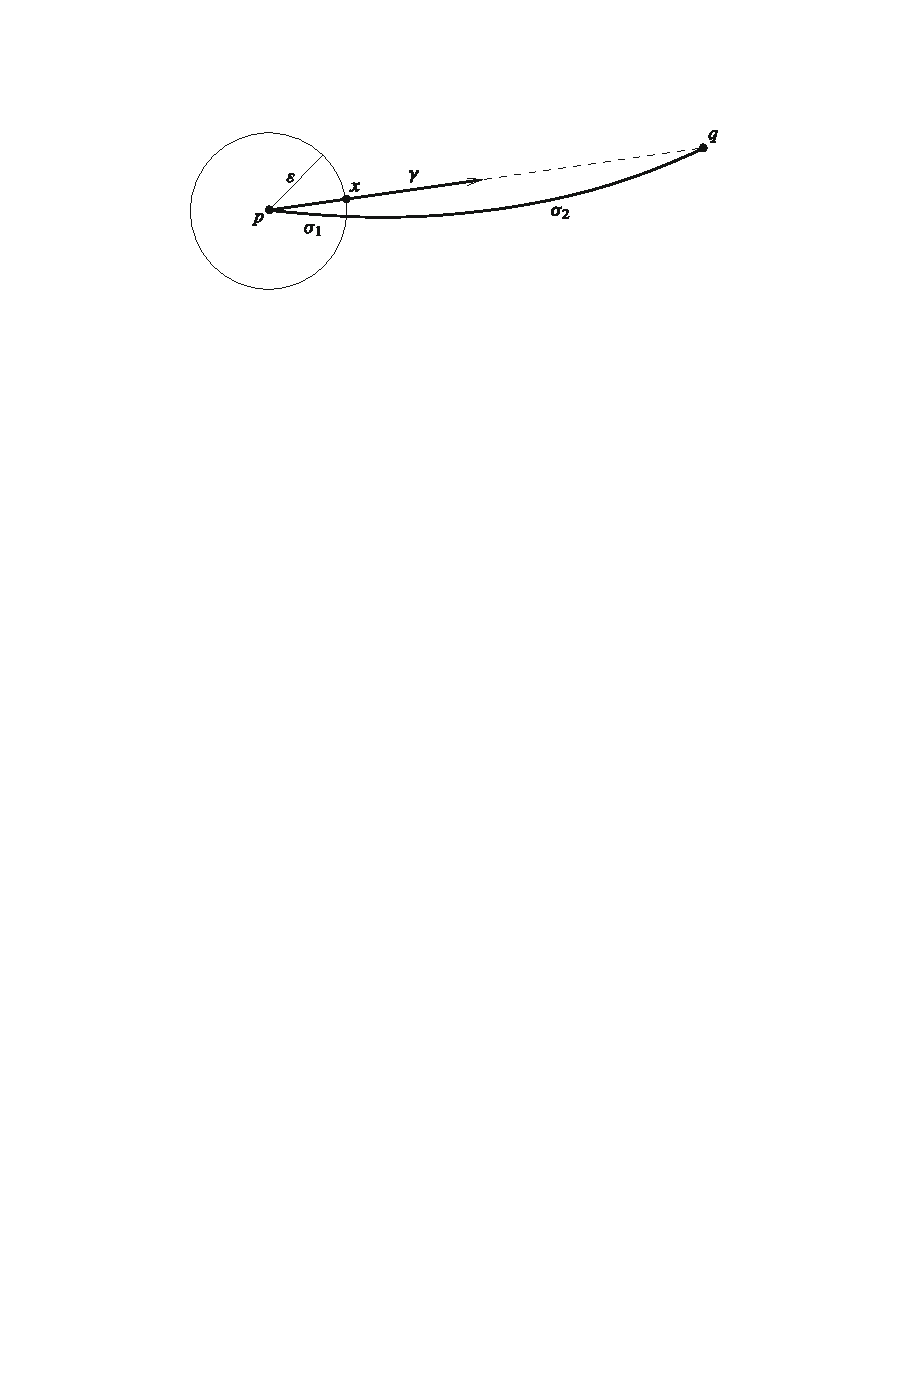
\includegraphics{pictures/Hopf-Rinow-lem-1}
\caption{Proof that $\gamma|_{[0,\eps]}$ aims at $q$.}
\end{figure}

To this end, let $\sigma:[a_0,b_0]\to M$ be any admissible curve from $p$ to $q$. Let $t_0$ be the first time $\sigma$ hits $S_\eps(p)$, and let $\sigma_1$ and $\sigma_2$ 
denote the restrictions of $\sigma$ to $[a_0,t_0]$ and $[t_0,b_0]$, respectively. Since every point in $S_\eps(p)$ is at a distance $\eps$ from $p$, we have 
\[L_g(\sigma_1)\geq d_g(p,\sigma(t_0))=d_g(p,x),\]
and by our choice of $x$ we have
\[L_g(\sigma_2)\geq d_g(\sigma(t_0),q)\geq d_g(x,q).\]
Putting these two inequalities together yields
\[L_g(\sigma)=L_g(\sigma_1)+L_g(\sigma_2)\geq d_g(p,x)+d_g(x,q).\]
Taking the infimum over all such $\sigma$, we find that $d_g(p,q)\geq d_g(p,x)+d_g(x,q)$. The opposite inequality is just the triangle inequality, so $(\ref{Riemann hopf-rinow lem-2})$ 
holds.\par
Now let $T=d_g(p,d)$ and
\[\mathcal{A}=\{b\in[0,T]:\text{$\gamma|_{[0,b]}$ aims at $q$}\}.\]
We have just shown that $\eps\in\mathcal{A}$. Let $A=\sup\mathcal{A}$. By continuity of the distance function, it is easy to see that $\mathcal{A}$ is closed in $[0,T]$, and 
therefore $A\in\mathcal{A}$. If $A=T$, then $\gamma|_{[0,T]}$ is a geodesic of length $T=d_g(p,q)$ that aims at $q$, and by the remark above we are done. So we assume 
$A<T$ and derive a contradiction.
\begin{figure}[htbp]
\centering
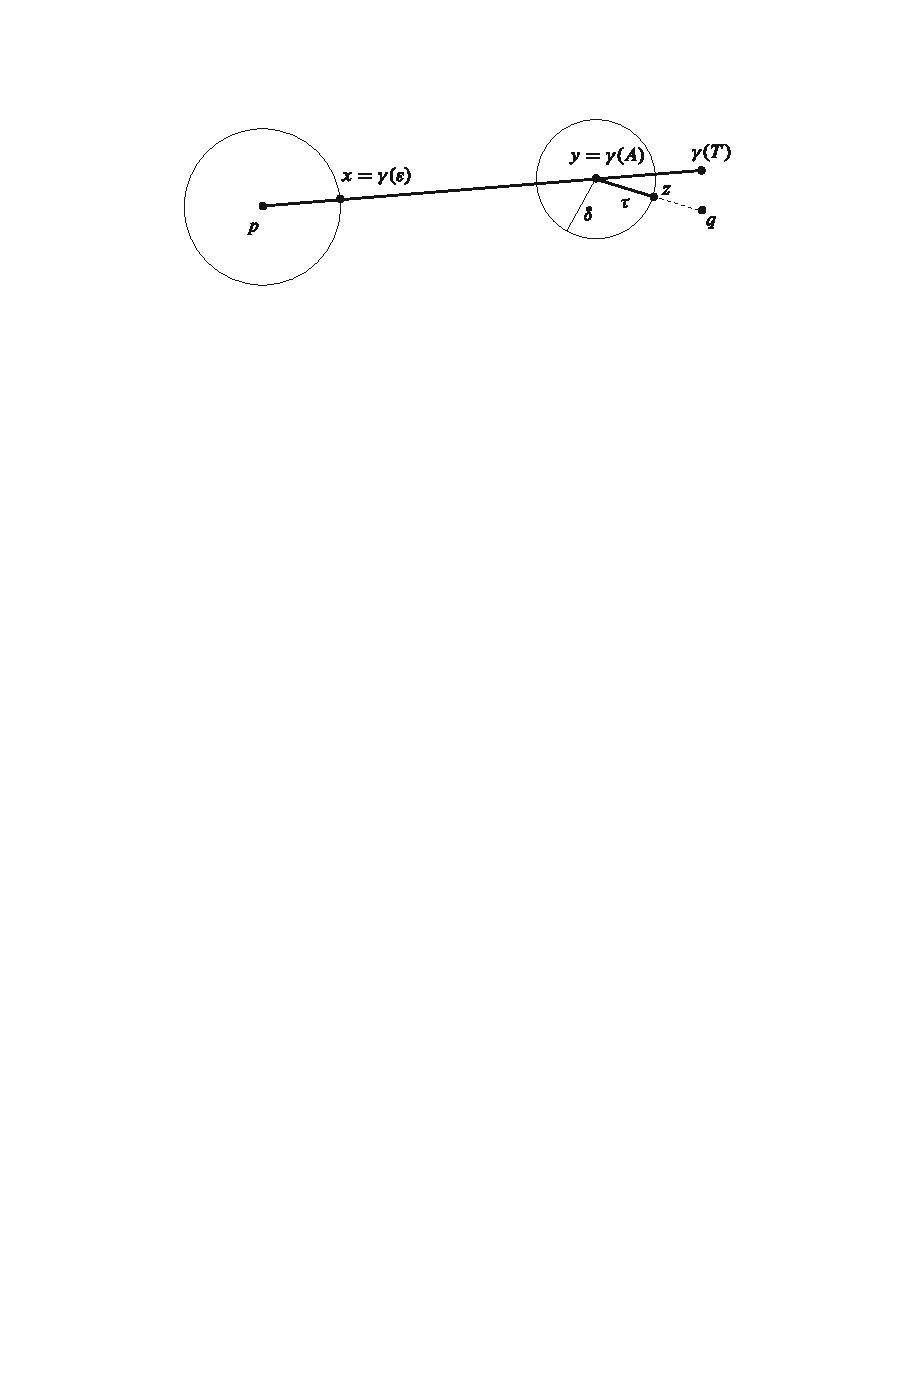
\includegraphics{pictures/Hopf-Rinow-lem-2}
\caption{Proof that $A=T$.}
\end{figure}

Let $y=\gamma(A)$, and choose $\delta>0$ such that there is a closed geodesic ball $\widebar{B_{\delta}(y)}$ around $y$, small enough that it does not contain $q$. The fact that $A\in\mathcal{A}$ means that
\[d_g(p,q)=d_g(p,y)+d_g(y,q).\]
Let $z\in S_\delta(y)$ be a point where $d_g(z,q)$ attains its minimum, and let $\tau:[0,\delta]\to M$ be the unit-speed radial geodesic from $y$ to $z$. By exactly the same argument as before, $\tau$ aims at $q$, so
\begin{align}\label{Riemann hopf-rinow lem-3}
d_g(y,q)=d_g(y,z)+d_g(z,q).
\end{align}
By the triangle inequality
\begin{equation}\label{Riemann hopf-rinow lem-4}
\begin{aligned}
d_g(p,z)&\geq d_g(p,q)-d_g(z,q)\\
&=d_g(p,y)+d_g(y,q)-d_g(z,q)\\
&=d_g(p,y)+d_g(y,z)\\
&\geq d_g(p,z).
\end{aligned}
\end{equation}
Therefore, the admissible curve consisting of $\gamma|_{[0,A]}$ (of length $A$) followed by $\tau$ (of length $\delta$) is a minimizing curve from $p$ to $z$. This means that it has no corners, so $z$ must lie on $\gamma$, and in fact, $z=\gamma(A+\delta)$. But then $(\ref{Riemann hopf-rinow lem-4})$ says that
\[d_g(p,q)=d_g(p,z)+d_g(q,z),\]
so $\gamma|_{[0,A+\delta]}$ aims at $q$ and $A+\delta\in\mathcal{A}$, which is a contradiction. This completes the proof of (a).
\begin{figure}[htbp]
\centering
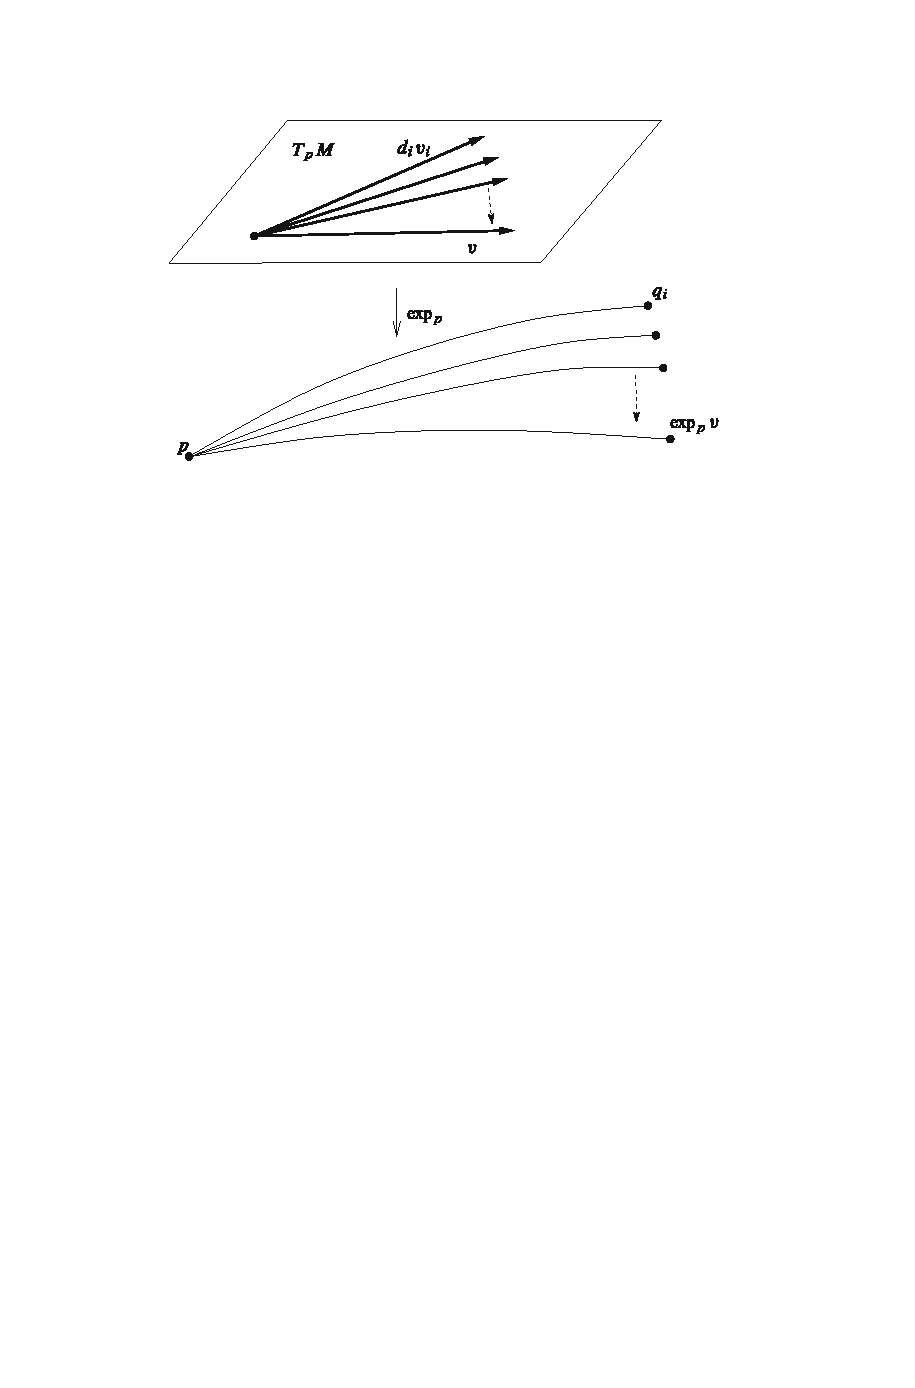
\includegraphics{pictures/Hopf-Rinow-lem-3}
\caption{Cauchy sequences converge.}
\end{figure}

To prove (b), we need to show that every Cauchy sequence in $M$ converges. Let $(q_i)$ be a Cauchy sequence in $M$. For each $i$, let $\gamma_i(t)=\exp_p(tv_i)$ be a 
unit-speed minimizing geodesic from $p$ to $q_i$, and let $d_i=d_g(p,q_i)$, so that $q_i=\exp_p(d_iv_i)$. The sequence $(d_i)$ is bounded in $\R$ (because Cauchy 
sequences in a metric space are bounded), and the sequence $(v_i)$ consists of unit vectors in $T_pM$, so the sequence of vectors $(d_iv_i)$ in $T_pM$ is bounded. 
Therefore a subsequence $(d_{i_k}v_{i_k})$ converges to some $v\in T_pM$. By continuity of the exponential map, $q_{i_k}=\exp_p(d_{i_k}v_{i_k})\to\exp_p(v)$ and since the 
original sequence $(q_i)$ is Cauchy, it converges to the same limit.
\end{proof}
\begin{theorem}[\textbf{Hopf-Rinow}]
Let $(M,g)$ be a connected Riemannian manifold. Then the following statements are equivalent:
\begin{itemize}
\item[(\rmnum{1})] $M$ is metrically complete.
\item[(\rmnum{2})] $M$ geodesically complete.
\item[(\rmnum{3})] There exists $p\in M$ so that $\exp_p$ is defined on the whole tangent space $T_pM$.
\item[(\rmnum{4})] Any bounded closed subset in $M$ is compact.
\end{itemize}
Moreover, each of the previous statements implies that any two points in $M$ can be joined by a minimizing geodesic segment
\end{theorem}
\begin{remark}
The condition that any tow points can be connected by a minimizing geodesic does not implies that $M$ is complete. For example, this statement is true in the Euclidean 
ball $\B^n\sub\R^n$, but it is not complete.\par
Also, the equivalence of the completeness and the Heine-Borel property is not valid in general metric spaces. For example, one can consider a countable infinite set 
$\{x_n:n\in\N\}$ and define a metric on it via $d(x_i,x_j)=1$ for all $i\neq j$ (discrete metric). In this space, the only Cauchy sequences are eventually-constant 
sequences which of course converge. However, the whole space is closed and bounded but not compact. So as metric spaces, Riemannian manifolds are special (and nice) 
metric spaces.
\end{remark}
\begin{proof}
Clearly we only need to prove the equivalence of (\rmnum{1})--(\rmnum{4}) in view of Lemma~\ref{Riemann hopf-rinow lem}. Moreover, the implications (\rmnum{2})$\Rightarrow(\rmnum{3})\Rightarrow$(\rmnum{1}) are immediate by the same lemma, and (\rmnum{4})$\Rightarrow$(\rmnum{1}) is a standard result for metric spaces.\par
Now we show (\rmnum{1})$\Rightarrow$(\rmnum{2}). Suppose $M$ is metrically complete, and assume for the sake of contradiction that it is not geodesically complete. Then 
there is some unit-speed geodesic $\gamma:[0,b)\to M$ that has no extension to a geodesic on any interval $[0,b_0)$ for $b_0>b$. Let $(t_i)$ be any increasing sequence 
in $[0,b)$ that approaches $b$, and set $q_i=\gamma(t_i)$. Since $\gamma$ is parametrized by arc length, the length of $\gamma|_{[t_i,t_{j}]}$ is exactly $t_{i+1}-t_i$, 
so $d_g(q_i,q_j)\leq|t_i,t_j|$ and $(q_i)$ is a Cauchy sequence inM. By completeness, $(q_i)$ converges to some point $q\in M$.\par
Let $W$ be a uniformly $\delta$-normal neighborhood of $q$ for some $\delta>0$. Choose $j$ large enough that $t_j>b-\delta$ and $q_j\in W$. The fact that $B_{\delta}(q_j)$ 
is a geodesic ball means that every unit-speed geodesic starting at $q_j$ exists at least for $t\in[0,\delta)$. In particular, this is true of the geodesic $\sigma$ with 
$\sigma(0)=q_j$ and $\sigma'(0)=\gamma'(t_j)$. Define $\tilde{\gamma}:[0,t_j+\delta)\to M$ by
\[\tilde{\gamma}(t)=\begin{cases}
\gamma(t)&t\in[0,b);\\
\sigma(t-t_j)&t\in(t_j,t_j+\delta)
\end{cases}\]
Note that both expressions on the right-hand side are geodesics, and they have the same position and velocity when $t=t_j$. Therefore, by uniqueness of geodesics, the 
two definitions agree where they overlap. Since $t_j+\delta>b$, $\tilde{\gamma}$ is an extension of $\gamma$ past $b$, which is a contradiction.\par
Finally, we show (\rmnum{3})$\Rightarrow$(\rmnum{4}). Suppose that there exists $p\in M$ so that $\exp_p$ is defined on the whole tangent space $T_pM$. Let $K\sub M$ be 
a bounded closed set. Then there exists a constant $C>0$ so that $d(p,k)<C$ for all $k\in K$. Then according to (\rmnum{3}), $K$ is contained in the closed geodesic ball 
$\widebar{B_{C}(p)}$, which is compact since $B_{C}(0)$ is compact in $T_pM$. Thus $K$, as a closed subset of a compact set, is compact.
\end{proof}
\begin{corollary}
If $M$ is a compact Riemannian manifold, then every maximal geodesic in $M$ is defined for all time.
\end{corollary}
Now we use the Hopf-Rinow theorem to prove the following important theorem about Riemannian covering maps.
\begin{theorem}\label{Riemann local isometry complete is cover}
Suppose $(\widetilde{M},\tilde{g})$ and $(M,g)$ are connected Riemannian manifolds with $\widetilde{M}$ complete, and $\pi:\widetilde{M}\to M$ is a local isometry. Then $M$ is complete and $\pi$ is a Riemannian covering map.
\end{theorem}
\begin{proof}
A fundamental property of covering maps is the path-lifting property: if $\pi$ is a covering map, then every continuous path $\gamma:I\to M$ lifts to a path $\tilde{\gamma}$ in $\widetilde{M}$ such that $pi\circ\tilde{\gamma}=\gamma$. We begin by proving that $\pi$ possesses the path-lifting property for geodesics: if $p\in M$ is a point in the image of $\pi$, $\gamma:I\to M$ is any geodesic starting at $p$, and $\tilde{p}$ is any point in $\pi^{-1}(p)$, then $\gamma$ has a unique lift starting at $\tilde{p}$. The lifted curve is necessarily also a geodesic because $\gamma$ is a local isometry.
\begin{figure}[htbp]
\centering
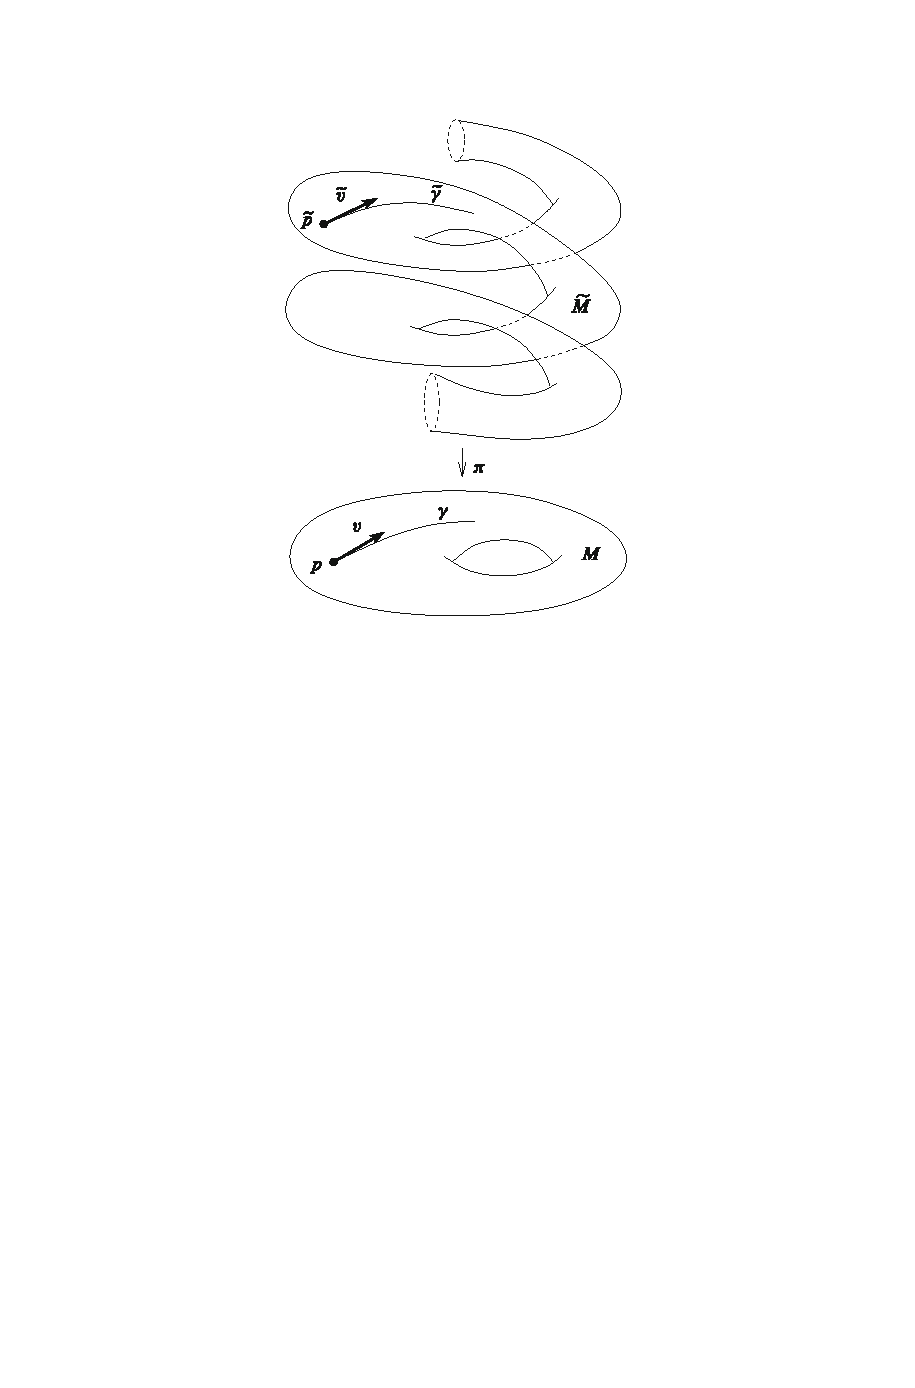
\includegraphics{pictures/local-isometry-cover}
\caption{Lifting geodesics.}
\end{figure}

To prove the path-lifting property for geodesics, suppose $p\in\pi(\widetilde{M})$ and $\tilde{p}\in\pi^{-1}(M)$, and let $\gamma:I\to M$ be any geodesic with $p=\gamma(0)$. Let $v=\gamma'(0)$ and $\tilde{v}=(d\pi_{\tilde{p}})^{-1}(v)\in T_{\tilde{p}}\widetilde{M}$ (which is well defined because $d\pi_{\tilde{p}}$ is an isomorphism), and let $\tilde{\gamma}$ be the geodesic in $\widetilde{M}$ with initial point $\tilde{p}$ and initial velocity $\tilde{v}$. Because $\widetilde{M}$ is complete, $\tilde{\gamma}$ is defined on all of $\R$. Since $\pi$ is a local isometry, it takes geodesics to geodesics; and since by construction $\pi(\tilde{\gamma}(0))=\gamma(0)$ and $d\pi_{\tilde{p}}(\tilde{\gamma}'(0))=\gamma'(0)$, we must have $\pi\circ\tilde{\gamma}=\gamma$ on $I$, so $\tilde{\gamma}|_I$ is a lift of $\gamma$ starting at $\tilde{p}$.\par
To show that $M$ is complete, let $p$ be any point in the image of $\pi$. If $\gamma:I\to M$ is any geodesic starting at $p$, then $\gamma$ has a lift $\tilde{\gamma}:I\to\widetilde{M}$. Because $\widetilde{M}$ is complete, $\pi\circ\tilde{\gamma}$ is a geodesic defined for all $t$ that coincides with $\gamma$ on $I$, so $\gamma$ extends to all of $\R$. 
Thus $M$ is complete by Hopf-Rinow Theorem.\par
Next we show that $\gamma$ is surjective. Choose some point $\tilde{p}\in\widetilde{M}$, write $p=\pi(\tilde{p})$, and let $q\in M$ be arbitrary. Because $M$ is connected and complete, there is a minimizing unit-speed geodesic segment $\gamma$ from $p$ to $q$. Letting $\tilde{\gamma}$ be the lift of $\gamma$ starting at $\tilde{p}$ and $r=d_g(p,q)$, we have $\pi(\tilde{\gamma}(r))=\gamma(r)=q$, so $q$ is in the image of $\pi$.\par
To show that $\pi$ is a smooth covering map, we need to show that every point of $M$ has a neighborhood $U$ that is evenly covered, which means that $\pi^{-1}(U)$ is a disjoint union of connected open sets $\widetilde{U}_\alpha$ such that $\pi|_{\widetilde{U}_\alpha}$ is a diffeomorphism. We will show, in fact, that every geodesic ball is evenly covered.
\begin{figure}[htbp]
\centering
\begin{minipage}[b]{200pt}
\centering
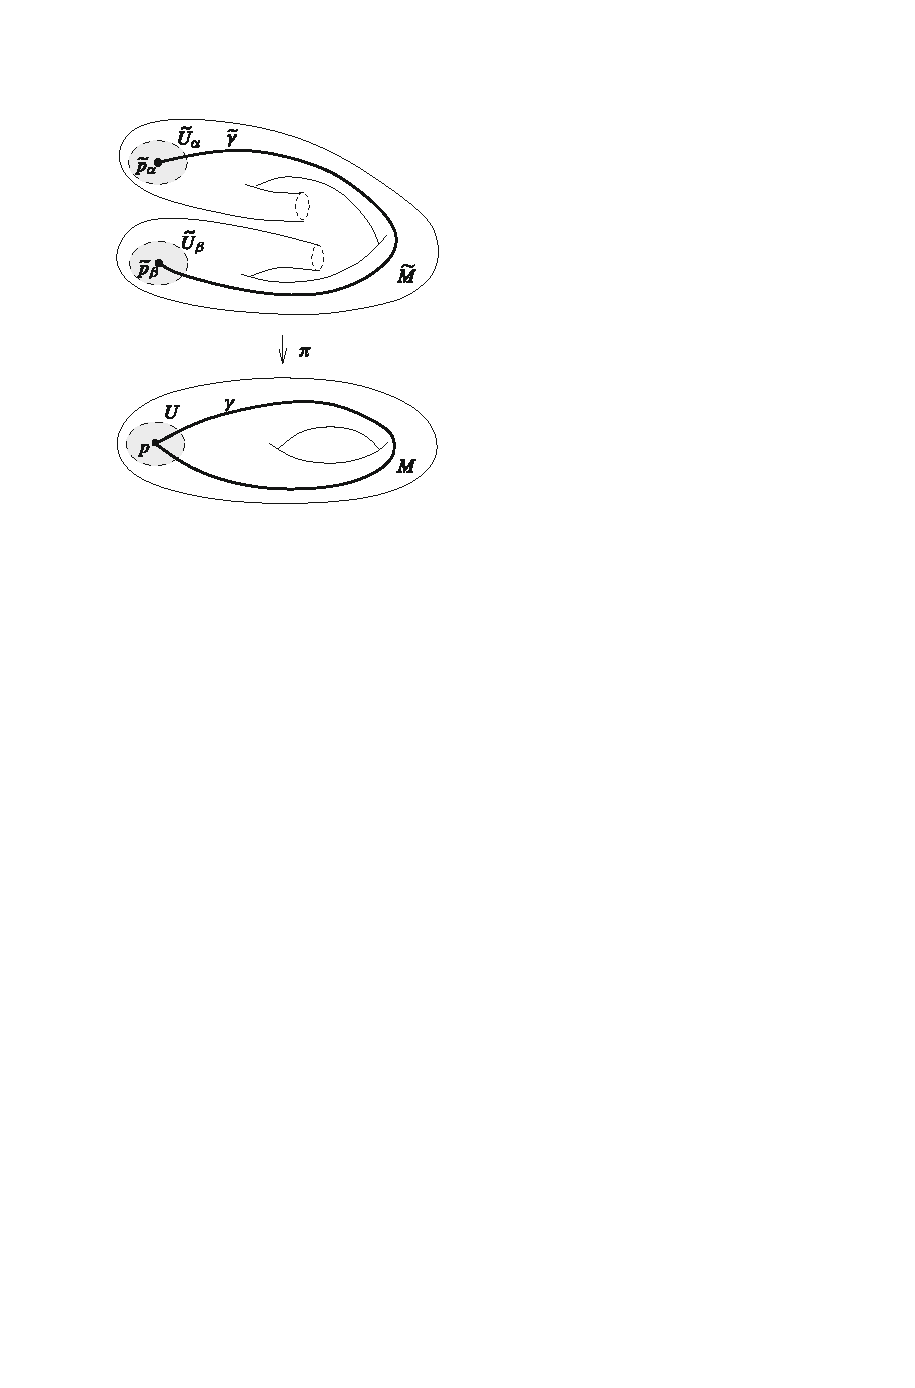
\includegraphics{pictures/local-isometry-cover-2}
\caption{Proof that $\widetilde{U}_\alpha\cap\widetilde{U}_\beta=\emp$.}
\end{minipage}
\hspace{20pt}
\begin{minipage}[b]{200pt}
\centering
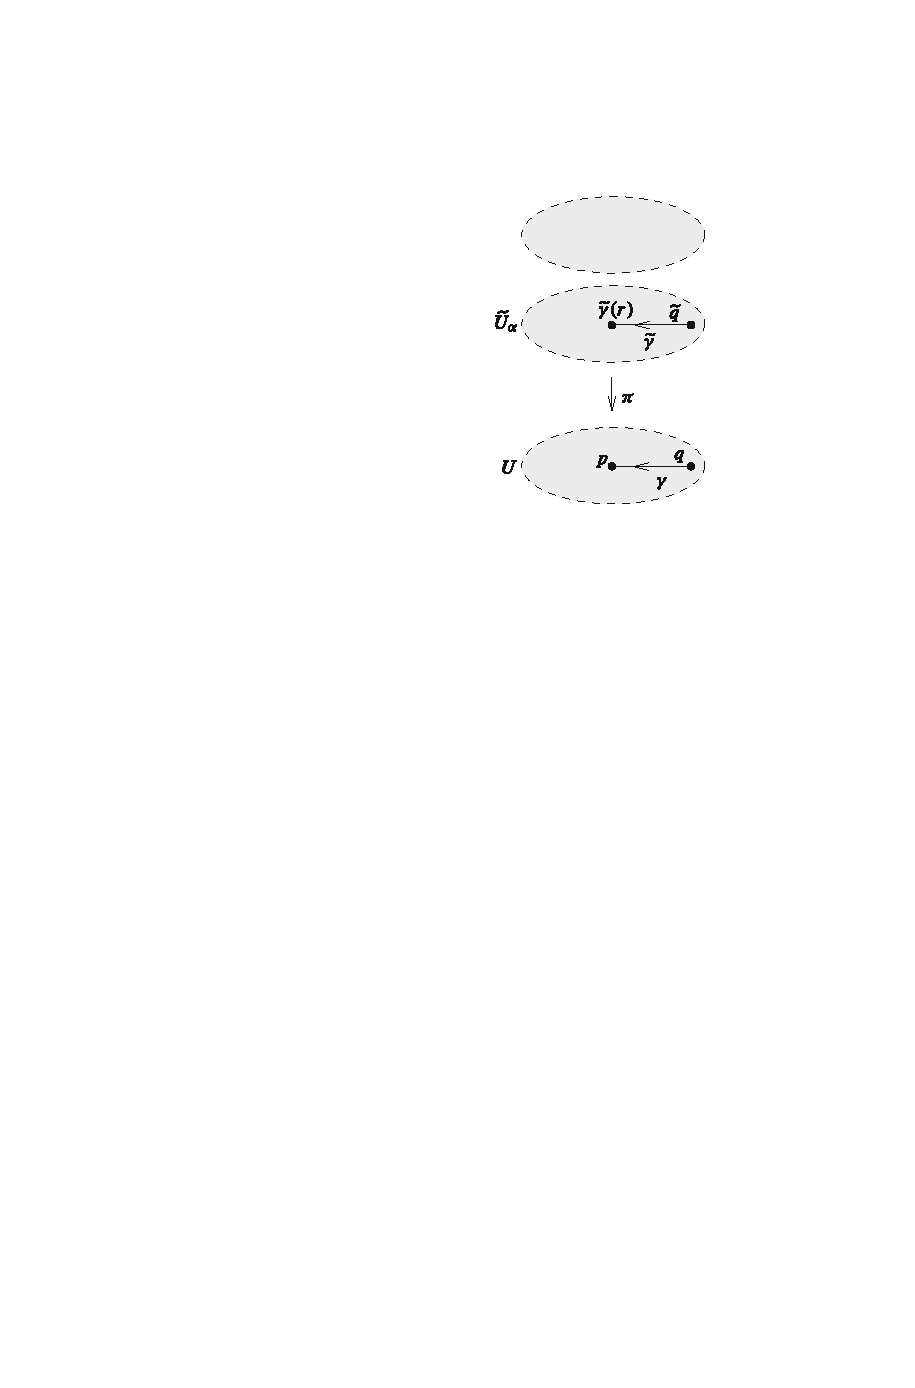
\includegraphics{pictures/local-isometry-cover-3}
\caption{Proof that $\pi^{-1}(U)\sub\bigcup_\alpha\widetilde{U}_\alpha$.}
\end{minipage}
\end{figure}

Let $p\in M$, and let $U=B_{\eps}(p)$ be a geodesic ball centered at $p$. Write $\pi^{-1}(p)=\{\tilde{p}_\alpha\}_{\alpha\in A}$, and for each $\alpha$ let $\widetilde{U}_\alpha$ 
denote the metric ball of radius $\eps$ around $\tilde{p}_\alpha$ (we are not claiming that $\widetilde{U}_\alpha$ is a geodesic ball). The first step is to show that the various sets $\widetilde{U}_\alpha$ are disjoint. For every $\alpha\neq\beta$, there is a minimizing geodesic segment $\tilde{\gamma}$ from $\tilde{p}_\alpha$ to $\tilde{p}_\beta$ because $\widetilde{M}$ is complete. The projected curve $\pi\circ\tilde{\gamma}$ is a geodesic segment that starts and ends at $p$, whose length is the same as that of $\tilde{\gamma}$. Such a geodesic must leave $U$ and reenter it (since all geodesics passing through $p$ and lying in $U$ are radial line segments), and thus must have length at least $2\eps$. This means that $d_g(\tilde{p}_\alpha,\tilde{p}_\beta)$, and thus by the 
triangle inequality, $\widetilde{U}_\alpha\cap\widetilde{U}_\beta=\emp$.\par
The next step is to show that $\pi^{-1}=\bigcup_\alpha\widetilde{U}_\alpha$. If $\tilde{q}$ is any point in $\widetilde{U}_\alpha$, then there is a geodesic $\tilde{\gamma}$ of length less than $\eps$ from $\tilde{p}_\alpha$ to $\tilde{q}$, and then $\pi\circ\tilde{\gamma}$ is a geodesic of the same length from $p$ to $\pi(\tilde{q})$, showing that $\pi(\tilde{q})\in U$. It follows that $\bigcup_\alpha\widetilde{U}_\alpha\sub\pi^{-1}(U)$.\par
Conversely, suppose $\tilde{q}\in\pi^{-1}(U)$, and set $q=\pi(\tilde{q})$. This means that $q\in U$, so there is a minimizing radial geodesic $\gamma$ in $U$ from $q$ to $p$, and $r=d_g(q,p)<\eps$. Let $\tilde{\gamma}$ be the lift of $\gamma$ starting at $\tilde{q}$. It follows that $\pi(\tilde{\gamma}(r))=\gamma(r)=p$. Therefore $\tilde{\gamma}(r)=\tilde{p}_\alpha$ for some $\alpha$, and $d_{\tilde{g}}(\tilde{q},\tilde{p}_\alpha)\leq L_g(\tilde{\gamma})=r<\eps$, so $\tilde{q}\in\widetilde{U}_\alpha$.\par
It remains only to show that $\pi:\widetilde{U}_\alpha\to U$ is a diffeomorphism for each $\alpha$. It is certainly a local diffeomorphism (because $\pi$ is). It is bijective because its inverse can be constructed explicitly: it is the map sending each radial geodesic starting at $p$ to its lift starting at $\tilde{p}_\alpha$. This completes the proof.
\end{proof}
\begin{corollary}\label{Riemann cover complete iff}
Suppose $\widetilde{M}$ and $M$ are connected Riemannian manifolds, and $\pi:\widetilde{M}\to M$ is a Riemannian covering map. Then $M$ is complete if and only if $\widetilde{M}$ is complete.
\end{corollary}
\begin{proof}
A Riemannian covering map is, in particular, a local isometry. Thus if $\widetilde{M}$ is complete, $\pi$ satisfies the hypotheses of 
Theorem~\ref{Riemann local isometry complete is cover}, which implies that $M$ is also complete.\par
Conversely, suppose $M$ is complete. Let $\tilde{p}\in\widetilde{M}$ and $\tilde{v}\in T_{\tilde{p}}\widetilde{M}$ be arbitrary, and let $p=\pi(\tilde{p})$ and $v=d\pi_{\tilde{p}}(\tilde{v})$. Completeness of $M$ implies that the geodesic $\gamma$ with $\gamma(0)=p$ and $\gamma'(0)=v$ is defined for all $t\in\R$, and then its lift $\tilde{\gamma}:\R\to\widetilde{M}$ starting at $\tilde{p}$ is a geodesic in $\widetilde{M}$ with initial velocity $\tilde{v}$, also defined for all $t$.
\end{proof}
The Hopf-Rinow theorem shows that any two points in a complete, connected Riemannian manifold can be joined by a minimizing geodesic segment. The next proposition gives a refinement of that statement.
\begin{proposition}\label{Riemann geodesic in homotopy class}
Suppose $(M,g)$ is a complete, connected Riemannian manifold, and $p,q\in M$. Every path-homotopy class of paths from $p$ to $q$ contains a geodesic segment $\gamma$ that minimizes length among all admissible curves in the same path-homotopy class.
\end{proposition}
\begin{proof}
Let $\pi:\widetilde{M}\to M$ be the universal covering manifold of $M$, endowed with the pullback metric $\tilde{g}=\pi^*g$. Given $p,q\in M$ and a path $\sigma:[0,1]\to M$ from $p$ to $q$, choose a point $\tilde{p}\in\pi^{-1}(p)$ and let $\tilde{\sigma}:[0,1]\to\widetilde{M}$ be the lift of $\sigma$ starting at $\tilde{p}$, and set $\tilde{q}=\tilde{\sigma}(1)$. By the Hopf-Rinow theorem, there is a minimizing $\tilde{g}$-geodesic segment $\tilde{\gamma}$ from $\tilde{p}$ to $\tilde{q}$, and because $\pi$ is a local isometry, $\pi\circ\tilde{\gamma}$ is a geodesic in $M$ from $p$ to $q$. If $\gamma_1$ is any other admissible curve from $p$ to $q$ in the same path-homotopy class, then by the monodromy theorem, its lift $\tilde{\gamma}_1$ starting at $\tilde{p}$ also ends at $\tilde{q}$. Thus $\tilde{\gamma}_1$ is no longer than $\tilde{\gamma}$, which implies $\gamma_1$ is no longer than $\gamma$.
\end{proof}
Suppose $(M,g)$ is a connected Riemannian manifold. A \textbf{closed geodesic} in $M$ is a nonconstant geodesic segment $\gamma:[a,b]\to M$ such that $\gamma(a)=\gamma(b)$ and $\gamma'(a)=\gamma'(b)$.
\begin{proposition}
A geodesic segment is closed if and only if it extends to a periodic geodesic defined on all of $\R$.
\end{proposition}
Round spheres have the remarkable property that all of their geodesics are closed when restricted to appropriate intervals. Of course, this is not typically the case, even 
for compact Riemannian manifolds; but it is natural to wonder whether closed geodesics exist in more general manifolds. Much work has been done in Riemannian geometry to 
determine how many closed geodesics exist in various situations. Here we can only touch on the simplest case.\par
A continuous path $\sigma:[0,1]\to M$ is called a \textbf{loop} if $\sigma(0)=\sigma(1)$. Two loops are said to be \textbf{freely homotopic} if they are homotopic 
through closed paths (but not necessarily preserving the base point). This is an equivalence relation on the set of all loops in $M$, and an equivalence class is 
called a \textbf{free homotopy class}. The \textbf{trivial free homotopy class} is the equivalence class of any constant path.
\begin{lemma}
Given a connected manifold $M$ and a point $x\in M$, then a loop based at $x$ represents the trivial free homotopy class if and only if it represents the identity 
element of $\pi_1(M,x)$.
\end{lemma}
\begin{proof}
Assume that a loop $\sigma$ based at $x$ is freely homotopic to the constant loop $c_y$ for $y\in M$, that is, there exists a homotopy $H:[0,1]\times[0,1]\to M$ satisfying
\[H(s,0)=\sigma(s),H(s,1)=y\for s\in[0,1],\quad H(0,t)=H(1,t) \for t\in[0,1].\]
Let $\gamma(t)=H(0,t)$, then we have $[\widebar{\gamma}\ast\sigma\ast\gamma]=[c_y]$. Then we get $[\sigma]=[\gamma]\ast[c_y]\ast[\widebar{\gamma}]=[c_x]$, so $\sigma$ represents the identity element of $\pi_1(M,x)$.
\end{proof}
The next proposition shows that closed geodesics are easy to find on compact Riemannian manifolds that are not simply connected.
\begin{proposition}
Suppose $(M,g)$ is a compact, connected Riemannian manifold. Every nontrivial free homotopy class in $M$ is represented by a closed geodesic that has minimum length among all admissible loops in the given free homotopy class.
\end{proposition}
\subsection{Distance functions}
Suppose $(M,g)$ is a connected Riemannian manifold and $S\sub M$ is any subset. For each point $x\in M$, we define the \textbf{distance from $\bm{x}$ to $\bm{S}$} to be
\[d_g(x,S)=\inf\{d_g(x,s):s\in S\}.\]
\begin{lemma}\label{Riemann distance function lem}
Suppose $(M,g)$ is a connected Riemannian manifold and $S\sub M$ is any subset.
\begin{itemize}
\item[(a)] $d_g(x,S)\leq d_g(x,y)+d_g(y,S)$ for all $x,y\in M$.
\item[(b)] $x\mapsto d_g(x,S)$ is a continuous function on $M$.
\end{itemize}
\end{lemma}
\begin{proof}
For all $x,y\in M$ and $s\in S$ we have
\[d_g(x,s)\leq d_g(x,y)+d_g(y,s).\]
Therefore $d_g(x,S)\leq d_g(x,y)+d_g(y,S)$. With this, we then get
\[|d_g(x,S)-d_g(y,S)|\leq d_g(x,y),\]
so $d_g(\cdot, S)$ is continuous.
\end{proof}
The simplest example of a distance function occurs when the set $S$ is just a singleton, $S=\{p\}$. Inside a geodesic ball around $p$, Corollary~\ref{Riemann distance is radial distance} 
shows that $d_g(x,S)=r(x)$, the radial distance function, and Corollary~\ref{Riemann radial distance grad} shows that it has unit gradient where it it smooth (everywhere 
inside the geodesic ball except at $p$ itself). The next theorem is a far-reaching generalization of that result.
\begin{theorem}\label{Riemann distance function grad}
Suppose $(M,g)$ is a connected Riemannian manifold, $S\sub M$ is arbitrary, and $f:[0,\infty)\to M$ is the distance to $S$, that is, $f(x)=d_g(x,S)$ for all $x\in M$. If 
$f$ is continuously differentiable on some open subset $U\sub M\setminus S$, then $|\grad f|\equiv 1$ on $U$.
\end{theorem}
\begin{proof}
Suppose $U\sub M\setminus S$ is an open subset on which $f$ is continuously differentiable, and $x\in U$. We will show first that $|\grad f|_x|\leq 1$, and then that $|\grad f|_x|\geq 1$.\par
To prove the first inequality, we may assume $\grad f|_x\neq 0$, for otherwise the inequality is trivial. Let $v\in T_xM$ be any unit vector, and let $\gamma$ be the unit-speed 
geodesic with $\gamma(0)=x$ and $\gamma'(0)=v$. Then for every positive $t$ sufficiently small that $\gamma|_{[0,t]}$ is minimizing, Lemma~\ref{Riemann distance function lem} gives 
$d_g(x,S)\leq d_g(x,\gamma(t))+d_g(\gamma(t),S)$,  or equivalently $f(x)\leq t+f(\gamma(t))$. Therefore, since $f$ is differentiable at $x$,
\[\frac{d}{dt}\Big|_{t=0}f(\gamma(t))=\lim_{t\to 0^+}\frac{f(\gamma(t))-f(\gamma(0))}{t}\leq 1.\]
In particular, taking $v=(\grad f|_x)/|\grad f|_x|$ (the unit vector in the direction of $\grad f|_x$), we obtain
\[\frac{d}{dt}\Big|_{t=0}f(\gamma(t))=df_x(\gamma'(0))=\langle\grad f|_x,v\rangle=|\grad f|_x|.\]
This proves $|\grad f|_x|\leq 1$.\par
To prove the reverse inequality, assume for the sake of contradiction that $|\grad f|_x|<1$. Since we are assuming that $\grad f$ is continuous on $U$, there exist $\delta,\eps>0$ 
suchthat $\widebar{B_\eps(x)}$ is a closed geodesic ball contained in $U$ and $|\grad f|\leq 1-\delta$ on it. Let $c$ be a positive constant less than $\delta\eps$. By 
definition of $d_g(x,S)$, there is an admissible curve $\sigma:[0,b]\to M$ (which we may assume to be parametrized by arc length) such that $\sigma(0)=x,\sigma(b)\in S$ and
\[b-c=L_g(\sigma)-c<d_g(x,S)<L_g(\sigma)=b.\]
Since we are assuming $\widebar{B_\eps(x)}\sub U\sub M\setminus S$, we have that $b>\eps$, so $\sigma|_{[\eps,b]}$ is an admissible curve from $\sigma(\eps)$ to $S$. On 
the one hand,
\begin{align}\label{Riemann distance function lem-1}
f(\sigma(\eps))=d_g(\sigma(\eps),S)\leq L_g(\sigma|_{[\eps,b]})=b-\eps<d_g(x,S)+c-\eps=f(x)+c-\eps.
\end{align}
On the other hand, for $t\in[0,\eps]$, the fact that $\sigma(t)\in\widebar{B_\eps(x)}$ implies
\[\Big|\frac{d}{dt}f(\sigma(t))\Big|=|\langle\grad f|_{\sigma(t)},\sigma'(t)\rangle|\leq|\grad f|_{\sigma(t)}||\sigma'(t)|\leq 1-\delta.\]
Thus $f(\sigma(t))\geq f(x)-(1-\delta)t$ for all such $t$. In particular, for $t=\eps$, this means that
\begin{align}\label{Riemann distance function lem-2}
f(\sigma(\eps))\geq f(x)-(1-\delta)\eps.
\end{align}
Combining $(\ref{Riemann distance function lem-1})$ and $(\ref{Riemann distance function lem-2})$ yields $c>\delta\eps$, contradicting our choice of $c$.
\end{proof}
Motivated by the previous theorem, if $(M,g)$ is a Riemannian manifold and $U\sub M$ is an open subset, we define a \textbf{local distance function} on $U$ to be a 
continuously differentiable function $f:U\to\R$ such that $|\grad f|_g\equiv 1$ in $U$. First, we develop some important general properties of local distance functions.
\begin{theorem}\label{Riemann local distance function int-curve geodesic}
Suppose $(M,g)$ is a Riemannian manifold and $f$ is a smooth local distance function on an open subset $U\sub M$. Then $\nabla_{\grad f}(\grad f)=0$, and each integral 
curve of $\grad f$ is a unit-speed geodesic.
\end{theorem}
\begin{proof}
Let $F\in\X(U)$ denote the unit vector field $\grad f$. The definition of the gradient shows that for every vector field $W$, we have
\[Wf=df(W)=\langle F,W\rangle.\]
and therefore
\[Ff=\langle F,F\rangle=|\grad f|^2\equiv 1.\]
For every smooth vector field $W$ on $U$, we have
\begin{align*}
\langle W,\nabla_FF\rangle&=F\langle W,F\rangle-\langle\nabla_FW,F\rangle\\
&=FWf-\langle\nabla_WF,F\rangle-\langle[F,W],F\rangle\\
&=FWf-[F,W]f-\frac{1}{2}W\langle F,F\rangle\\
&=WFf-\frac{1}{2}W|F|^2\\
&=0.
\end{align*}
Since $W$ is arbitrary, this proves that $\nabla_FF=0$.\par
If $\gamma:I\to U$ is an integral curve of $F$, then the fact that $\gamma'$ is extendible implies
\[D_t\gamma'(t)=\nabla_{\gamma'}\gamma'(t)=\nabla_FF|_{\gamma(t)}=0,\]
so $\gamma$ is a geodesic.
\end{proof}
\begin{lemma}\label{Riemann local distance function lem}
Suppose $(M,g)$ is a Riemannian manifold, $K\sub M$, and $f:K\to\R$ is a continuous function whose restriction to some open set $W\sub K$ is a smooth local distance function. 
For every admissible curve $\sigma:[a_0,b_0]\to K$ such that $\sigma(a_0,b_0)\sub W$, we have
\[L_g(\sigma)\geq|f(\sigma(b_0))-f(\sigma(a_0))|.\]
\end{lemma}
\begin{proof}
This is proved exactly as in $(\ref{Riemann geodesic ball minimize-1})$, noting that the only properties of $r$ we used in that computation were that it is continuous on the image of $\sigma$ and continuously 
differentiable on $\sigma(a_0,b_0)$, and its gradient has unit length there.
\end{proof}
The next theorem and its corollary explain why the name "local distance function" is justified. Its proof is an adaptation of the proof of Proposition~\ref{Riemann geodesic ball radial is minimize}.
\begin{theorem}\label{Riemann local distance function is locally distance}
Suppose $(M,g)$ is a Riemannian manifold, $U\sub M$ is an open subset, $S\sub U$, and $f:U\to[0,\infty)$ is a continuous function such that $f^{-1}(0)=S$ and $f$ is a 
smooth local distance function on $U\setminus S$. Then there is a neighborhood $U_0\sub U$ of $S$ in which $f(x)$ is equal to the distance in $M$ from $x$ to $S$.
\end{theorem}
\begin{proof}
For each $p\in S$, there are positive numbers $\eps_p,\delta_p$ such that $B_{\eps_p}(p)$ is a uniformly $\delta_p$-normal geodesic ball and $B_{2\eps_p}(p)\sub U$. This 
means that $B_{\eps_p}(p)$ is contained in the open geodesic ball of radius $\delta_p$ around each of its points. In particular, $B_{\eps_p}(p)\sub B_{\delta}(p)$, which means that $\eps_p\leq\delta_p$, and thus every geodesic starting at a point of $B_{\eps_p}(p)$ is defined at least for $t\in(-\eps_p,\eps_p)$. Let $U_0$ be the union of all of the geodesic balls $B_{\eps_p}(p)$ for $p\in S$, which is a neighborhood of $S$ contained in $U$.\par
Let $x\in U_0$ be arbitrary, and let $c=f(x)$. We will show that $d_g(x,S)=f(x)$. If $x\in S$, then $d_g(x,S)=0=c$, so we may as well assume $x\notin S$.\par
There is some $p\in S$ such that $x\in B_{\eps_p}(p)$, which means that $d_g(x,S)<\eps_p$ and geodesics starting at $x$ are defined at least on $(-\eps_p,\eps_p)$. Let $\sigma:[0,b]\to B_{\eps_p}(p)$ be the radial geodesic segment from $p$ to $x$, we define
\[\mathcal{A}=\{t\in[0,b]:\sigma(t)\in S\},\]
and set $a=\sup\mathcal{A}$. Since $x\notin S$ and $S$ is closed, we have $a<b$, and $\sigma(a)\in S$. It follows from Lemma~\ref{Riemann local distance function lem} 
that 
\[L_g(\sigma)\geq L_g(\sigma|_{[a,b]})\geq |f(x)-f(\sigma(a))|=c,\]
and we conclude that $c\leq L_g(\sigma)<\eps_p$ as well.\par
Let $\gamma:(-\eps_p,\eps_p)\to U$ be the unit-speed geodesic starting at $x$ with initial velocity equal to $-\grad f|_x$. By 
Theorem~\ref{Riemann local distance function int-curve geodesic} and uniqueness of geodesics, $\gamma$ coincides with an integral curve of $-\grad f$ as long as 
$\gamma(t)\in U\setminus S$, which is to say as long as $f(\gamma(t))\neq 0$. For all such $t$ we have
\[\frac{d}{dt}f(\gamma(t))=\langle\grad f|_{\gamma(t)},\gamma'(t)\rangle=-|\grad f|_{\gamma(t)}|^2=-1.\]
so $f(\gamma(t))=c-t$ as long as $t<c$, and by continuity, $f(\gamma(c))=0$. This means that $f(\gamma(c))\in S$, and $\gamma|_{[0,c]}$ is a curve segment of length $c$ 
connecting $x$ with $S$, so $d_g(x,S)\leq c$.\par
To prove the reverse inequality, suppose $\sigma:[a,b]\to M$ is any admissible curve starting at $x$ and ending at a point of $S$. Assume first that $\sigma(t)\in U$ for 
all $t\in[a,b]$, and let $b_0\in[a,b]$ be the first time that $\sigma(b_0)\in S$. Then Lemma~\ref{Riemann local distance function lem} shows that
\[L_g(\sigma)\geq L_g(\sigma|_{[a,b_0]})=|f(\sigma(b_0))-f(\sigma(a))|=c.\]
On the other hand, suppose $\sigma(t)\in M\setminus U$ for some $t$. The fact $B_{\eps_p}(p)\sub B_{2\eps_p}(p)\sub U$ and the triangle inequality imply that there is 
a first time $b_0\in[a,b]$ such that $d_g(x,\sigma(b_0))\geq\eps_p$. Then 
\[L_g(\sigma)\geq L_g(\sigma|_{[a,b_0]})\geq d_g(x,\sigma(b_0))\geq\eps_p>c.\]
Taken together, these two inequalities show that $L_g(\sigma)\geq c$ for every such $\sigma$, which implies $d_g(x,S)\geq c$.
\end{proof}
\begin{corollary}\label{Riemann local distance level set}
Let $(M,g)$ be a Riemannian manifold, and let $f$ be a smooth local distance function on an open subset $U\sub M$. If $c$ is a real number such that $S=f^{-1}(c)$ is 
nonempty, then there is a neighborhood $U_0$ of $S$ in $U$ on which $|f(x)-c|$ is equal to the distance in $M$ from $x$ to $S$.
\end{corollary}
\begin{proof}
Observe that 
\[\grad |f(x)-c|=\frac{f(x)-c}{|f(x)-c|}\cdot\grad f.\]
Therefore $|f(x)-c|$ is a local distance function on $U\setminus S$.
\end{proof}
The following result is a global form of Theorem~\ref{Riemann local distance function is locally distance}.
\begin{theorem}
Suppose $(M,g)$ is a complete, connected Riemannian manifold, $S\sub M$ is a closed subset and $f:M\to\R$ is a continuous function such that $f^{-1}(0)=S$ and $f$ is smooth 
with unit gradient on $M\setminus S$. Then $f(x)=d_g(x,S)$ for all $x\in M$.
\end{theorem}
\begin{proof}
Let $x\in M\setminus S$ be arbitrary, and le $c=f(x)$. Let $\gamma:\R\to M$ be the unit-speed geodesic starting at $x$ with initial velocity equal to $-\grad f|_x$. By 
Theorem~\ref{Riemann local distance function int-curve geodesic} and uniqueness of geodesics, $\gamma$ coincides with an integral curve of $-\grad f$ as long as 
$\gamma(t)\in M\setminus S$, which is to say as long as $f(\gamma(t))\neq 0$. For all such $t$ we have
\[\frac{d}{dt}f(\gamma(t))=\langle\grad f|_{\gamma(t)},\gamma'(t)\rangle=-|\grad f|_{\gamma(t)}|^2=-1.\]
so $f(\gamma(t))=c-t$ as long as $t<c$, and by continuity, $f(\gamma(c))=0$. This means that $f(\gamma(c))\in S$, and $\gamma|_{[0,c]}$ is a curve segment of length $c$ 
connecting $x$ with $S$, so $d_g(x,S)\leq c$.\par
To prove the reverse inequality, suppose $\sigma:[a,b]\to M$ is any admissible curve starting at $x$ and ending at a point of $S$. Let $b_0\in[a,b]$ be the first time 
that $\sigma(b_0)\in S$. Then Lemma~\ref{Riemann local distance function lem} shows that
\[L_g(\sigma)\geq L_g(\sigma|_{[a,b_0]})=|f(\sigma(b_0))-f(\sigma(a))|=c.\]
Therefore $L_g(\sigma)\geq c$ for every such $\sigma$, which implies $d_g(x,S)\geq c$.
\end{proof}
\subsubsection{Distance functions for embedded submanifolds}
The most important local distance functions are those associated with embedded submanifolds. As we will see, such distance functions are always smooth near the manifold.\par
Suppose $(M,g)$ is a Riemannian $n$-manifold (without boundary) and $P\sub M$ is an embedded $k$-dimensional submanifold. Let $NP$ denote the normal bundle of $P$ in $M$, 
and let $U\sub M$ be a normal neighborhood of $P$ in $M$, which is the diffeomorphic image of a certain open subset $V\sub NP$ under the normal exponential map. (Such a 
neighborhood always exists by Theorem~\ref{Riemann tubular neighborhood}.) We begin by constructing generalizations of the radial distance function and radial vector 
field.
\begin{proposition}\label{Riemann distance subm}
Let $P$ be an embedded submanifold of a Riemannian manifold $(M,g)$ and let $U$ be any normal neighborhood of $P$ in $M$. There exist a unique continuous function $r:U\to[0,\infty)$ 
and smooth vector field $\partial_r$ on $U\setminus P$ that have the following coordinate representations in terms of any Fermi coordinates $(x,v)$ for $P$ on a subset $U_0\sub U$:
\begin{align}\label{Riemann distance subm-1}
r(x,v)&=\sqrt{(v^1)^2+\cdots+(v^{n-k})^2},
\end{align}
\begin{align}\label{Riemann distance subm-2}
\partial_r&=\frac{v^1}{r(x,v)}\frac{\partial}{\partial v^1}+\cdots+\frac{v^{n-k}}{r(x,v)}\frac{\partial}{\partial v^{n-k}}.
\end{align}
The function $r$ is smooth on $U\setminus P$, and $r^2$ is smooth on all of $U$.
\end{proposition}
\begin{proof}
The uniqueness, continuity, and smoothness claims follow immediately from the coordinate expressions $(\ref{Riemann distance subm-1})$ and $(\ref{Riemann distance subm-2})$, 
so we need only prove that $r$ and $\partial_r$ can be globally defined so as to have the indicated coordinate expressions in any Fermi coordinates.\par
Let $V\sub NP$ be the subset that is mapped diffeomorphically onto $U$ by the normal exponential map $E$. Define a function $\rho:V\to[0,\infty)$ by $\rho(p,v)=|v|_g$, 
and define $r:U\to[0,\infty)$ by $r=\rho\circ E^{-1}$. Any Fermi coordinates for $P$ are defined by choosing local coordinates $(x^1,\dots,x^k)$ for $P$ and a local 
orthonormal frame $(E_j)$ for $NP$, and assigning the coordinates $(x^1,\dots,x^k,v^1,\dots,v^{n-k})$ to the point $E(p,v^\alpha E_\alpha|_p)$. (Here we are using the 
summation convention with Greek indices running from $1$ to $n-k$.) Because the frame is orthonormal, for each $(p,v)=(p,v^\alpha E_\alpha|_p)\in V$ we have 
\[r(E(p,v))^2=\rho(p,v)^2=(v^1)^2+\cdots+(v^{n-k})^2,\]
which shows that $r$ has the coordinate representation $(\ref{Riemann distance subm-1})$.\par
To define $\partial_r$, let $q$ be an arbitrary point in $U\setminus P$. Then $q=\exp_p(tv)$ for a unique $(p,v)\in V$, and the curve $\gamma:[0,1]\to U$ given by $\gamma(t)=\exp_p(tv)$ 
is a geodesic from $p$ to $q$. Define
\begin{align}\label{Riemann distance subm-3}
\partial_r|_q=\frac{1}{r(q)}\gamma'(1),
\end{align}
which is independent of the choice of coordinates. Proposition~\ref{Riemann Fermi coordinate prop} shows that in any Fermi coordinates, if we write $v=v^\alpha E_\alpha|_p$, then $\gamma$ has the 
coordinate formula 
\[\gamma(t)=(x^1(p),\dots,x^k(p),tv^1,\dots,tv^{n-k}),\]
and therefore $\gamma'(t)=v^\alpha\partial/\partial v^\alpha|_{\gamma(t)}$. It follows that $\partial_r$ has the coordinate formula $(\ref{Riemann distance subm-2})$.
\end{proof}
By analogy with the special case in which $P$ is a point, we call $r$ the \textbf{radial distance function for $\bm{P}$} and $\partial_r$ the \textbf{radial vector field for $\bm{P}$}.
\begin{theorem}[\textbf{Gauss Lemma for Submanifolds}]\label{Guass lemma subm}
Let $P$ be an embedded submanifold of a Riemannian manifold $(M,g)$, let $U$ be a normal neighborhood of $P$ in $M$, and let $r$ and $\partial_r$ be defined as in 
Proposition~\ref{Riemann distance subm}. On $U\setminus P$, $\partial_r$ is a unit vector field orthogonal to the level sets of $r$.
\end{theorem}
\begin{proof}
The proof is a dressed-up version of the proof of the ordinary Gauss lemma. Let $q\in U\setminus P$ be arbitrary, and let $(x^1,\dots,x^k,v^1,\dots,v^{n-k})$ be the 
coordinate representation of $q$ in some choice of Fermi coordinates associated with a local orthonormal frame $(E_j)$ for $NP$. As in the proof of 
Proposition~\ref{Riemann distance subm}, $q=\gamma(1)$ where $\gamma$ is the geodesic $\exp_p(tv)$ for some $p\in P$ and $v=v^\alpha E_\alpha|_p\in N_pM$. Since the 
frame $(E_j)$ is orthonormal, we have
\[|\gamma'(0)|=|v|_g=\sqrt{(v^1)^2+\cdots+(v^{n-k})^2}=r(q).\]
Since geodesics have constant speed, it follows that $|\gamma'(1)|_g=r(q)$ as well, and then $(\ref{Riemann distance subm-3})$ shows that $\partial_r|_q$ is a unit 
vector.\par
Next we show that $\partial_r$ is orthogonal to the level sets of $r$. Suppose $q\in U\setminus P$, and write $q=\exp_{p_0}(v_0)$ for some $p_0\in P$ and $v_0\in N_{p_0}P$ 
with $v_0\neq 0$. The coordinate representation $(\ref{Riemann distance subm-1})$ shows that $r^{-1}(r(q))$ is a regular level set, and hence an embedded submanifold 
of $U$.\par
Let $w\in T_qM$ be an arbitrary vector tangent to this level set, and let $\sigma:(-\eps,\eps)\to U$ be a smooth curve lying in the same level set, with $\sigma(0)=q$ 
and $\sigma'(0)=w$. We can write $\sigma(s)=\exp_{x(s)}(v(s))$, where $x(s)\in P$ and $v(s)\in N_{x(s)}P$ with $|v(s)|_g=r(q)$. The initial condition $\sigma(0)=q$ 
translates to $x(0)=p_0$ and $v(0)=v_0$. Define a smooth one-parameter family of curves $\Gamma:(-\eps,\eps)\times[0,r(q)]\to M$ by
\[\Gamma(s,t)=\exp_{x(s)}\Big(\frac{t}{r(q)}v(s)\Big).\]
Since $|v(s)|_g=r(q)$, each $\Gamma_s$ is a unit-speed geodesic.\par
Note that $\Gamma(0,t)=\exp_{p_0}(tv_0/r(q))$, we have the following endpoint conditions:
\begin{align*}
&\partial_s\Gamma(0,0)=\frac{d}{ds}\Big|_{s=0}\exp_{x(s)}(0)=\frac{d}{ds}\Big|_{s=0}x(s)=x'(0);\\
&\partial_t\Gamma(0,0)=\frac{d}{dt}\Big|_{t=0}\exp_{p_0}\Big(\frac{v_0}{r(q)}t\Big)=\frac{v_0}{r(q)};\\
&\partial_s\Gamma(0,r(q))=\frac{d}{ds}\Big|_{s=0}\exp_{x(s)}(v(s))=\frac{d}{ds}\Big|_{s=0}\sigma(s)=w;\\
&\partial_t\Gamma(0,r(q))=\frac{d}{dt}\Big|_{t=r(q)}\exp_{p_0}\Big(\frac{v_0}{r(q)}t\Big)=\partial_r|_q.
\end{align*}
Then the same computation as in $(\ref{Guass lemma-1})$ shows that $(d/dt)\langle\partial_s\Gamma,\partial_t\Gamma\rangle=0$, and therefore
\[\langle w,\partial_r|_q\rangle=\langle\partial_s\Gamma(0,r(q)),\partial_t\Gamma(0,r(q))\rangle=\langle\partial_s\Gamma(0,0),\partial_t\Gamma(0,0)\rangle=\frac{1}{r(q)}\langle x'(0),v_0\rangle,\]
which is zero because $x'(0)$ is tangent to $P$ and $v_0$ is normal to it. This proves that $\partial_r$ is orthogonal to the level sets of $r$.
\end{proof}
\begin{corollary}\label{Riemann distance subm prop}
Assume the hypotheses of Theorem~\ref{Guass lemma subm}.
\begin{itemize}
\item[(a)] $\partial_r$ is equal to the gradient of $r$ on $U\setminus P$.
\item[(b)] $r$ is a local distance function.
\item[(c)] Each unit-speed geodesic $\gamma:[a,b)\to U$ with $\gamma'(a)$ normal to $P$ coincides with an integral curve of $\partial_r$ on $(a,b)$.
\item[(d)] $P$ has a tubular neighborhood in which the distance in $M$ to $P$ is equal to $r$.
\end{itemize}
\end{corollary}
\begin{proof}
By direct computation in Fermi coordinates using formulas $(\ref{Riemann distance subm-1})$ and $(\ref{Riemann distance subm-2})$, $\partial_r(r)=1$, which is equal to 
$|\partial_r|^2$ by the previous theorem. Thus $\partial_r=\grad r$ on $U\setminus P$ by Exercise~\ref{Riemann grad prop}. Because $\grad r$ is a unit vector field, $r$ is a local distance function. By Proposition~\ref{Riemann local distance function int-curve geodesic}, the geodesics in $U$ that start normal to $P$ are represented in any Fermi coordinates by $(x^1(p),\dots,x^k(p),tv^1,\dots,tv^{n-k})$, and such a geodesic has unit speed if and only if $(v^1)^2+\cdots+(v^{n-k})^2=1$. Another direct computation shows that each such curve is an integral curve of $\partial_r$ wherever $r\neq 0$.\par
Finally, to prove (d), note that Theorem~\ref{Riemann local distance function is locally distance} shows that there is some neighborhood $\widetilde{U}_0$ of $P$ in $M$ on which  $r(x)=d_g(x,P)$; if we take $U_0$ to be a tubular neighborhood of $P$ in $\widetilde{U}_0$, then $U_0$ satisfies the conclusion.
\end{proof}
When $P$ is compact, we can say more.
\begin{theorem}
Suppose $(M,g)$ is a connected Riemannian manifold, $P\sub M$ is a compact submanifold, and $U_\eps$ is an $\eps$-tubular neighborhood of $P$. Then $U_\eps$ is also an 
$\eps$-neighborhood in the metric space sense, and inside $U_\eps$, the distance in $M$ to $P$ is equal to the function $r$ defined in Proposition~\ref{Riemann distance subm}.
\end{theorem}
\begin{proof}
First we show that $r$ can be extended continuously to $\-bar{U}_\eps$ by setting $r(q)=\eps$ for $q\in\partial U_\eps$. Indeed, suppose $q\in\partial U_\eps$ and 
$q_i$ is any sequence of points in $U_\eps$ converging to $q$. Then $\varlimsup_ir(q_i)\leq\eps$ because $r(q_i)<\eps$ for each $i$. Let $c=\varliminf_ir(q_i)$, we will 
prove the result by showing that $c=\eps$. Suppose for the sake of contradiction that $c<\eps$. By passing to a subsequence, we may assume that $r(q_i)\to c$. We can 
write $q_i=\exp_{p_i}(v_i)$ for $p_i\in P$ and $v_i\in N_{p_i}P$, and because $P$ is compact and $\lim_i|v|_i=\lim_ir(q_i)\to c$, we can pass to a further subsequence 
and assume that $(p_i,v_i)\to(p,v)\in NP$ with $|v|_g=c<\eps$. Then we have $q=\lim_iq_i=\lim_i\exp_{p_i}(v_i)=\exp_pv$, which lies in the open set $U_\eps$, 
contradicting our assumption that $q=\partial U_\eps$. Henceforth, we regard $r$ as a continuous function on $\widebar{U}_\eps$.\par
Now to prove the theorem, let $W_\eps$ denote the $\eps$-neighborhood of $P$ in the metric space sense. Suppose first that $q\in M\setminus U_\eps$, and suppose 
$\sigma:[a,b]\to M$ is any admissible curve from a point of $P$ to $q$. There is a first time $b_0\in[a,b]$ that $\sigma(b_0)\in\partial U_\eps$, and then Lemma~\ref{Riemann local distance function lem} 
shows that
\[L_g(\sigma)\geq L_g(\sigma|_{[a,b_0]})\geq|r(\sigma(b_0))-r(\sigma(a))|=\eps.\]
Thus $q\notin U\eps\Rightarrow q\notin W_\eps$, or equivalently $W\eps\sub U_\eps$.\par
Conversely, suppose $q\in U_\eps$. Then $q$ is connected to $P$ by a geodesic segment of length $r(q)$, so $d_g(q,P)\leq r(q)$. To prove the reverse inequality, suppose 
$\sigma:[a,b]\to M$ is any admissible curve starting at a point of $P$ and ending at $q$. If $\sigma(t)$ remains in $U_\eps$ for all $t\in[a,b]$, then Lemma~\ref{Riemann local distance function lem} 
shows that
\[L_g(\sigma)\geq L_g(\sigma|_{[a_0,b]})\geq|r(\sigma(b))-r(\sigma(a_0))|=r(q),\]
where $a_0$ is the last time that $\sigma(a_0)\in P$. On the other hand, if $\sigma(t)$ does not remain in $U_\eps$, then there is a first time $b_0$ such that $\sigma(b_0)\in\partial U_\eps$, 
and the argument in the preceding paragraph shows that $L_g(\sigma)\geq\eps>r(q)$. Thus $d_g(q,P)=r(q)$ for all $q\in U_\eps$. Since $r(q)<\eps$ for all such $q$, it 
follows also that $U_\eps\sub W_\eps$.
\end{proof}
\subsection{Semigeodesic coordinates}
Local distance functions can be used to build coordinate charts near submanifolds in which the metric has a particularly simple form. We begin by describing the kind of 
coordinates we are looking for.\par
Let $(M,g)$ be an $n$-dimensional Riemannian manifold. Smooth local coordinates $(x^1,\dots,x^n)$ on an open subset $U\sub M$ are called 
\textbf{semigeodesic coordinates} if each $x^n$-coordinate curve $t\mapsto(X^1,\dots,x^{n-1},t)$ is a unit-speed geodesic that meets each level set of $x^n$ orthogonally.\par
Because of the distinguished role played by the last coordinate function, we will use the summation convention with Latin indices running from $1$ to $n$ and Greek 
indices running from $1$ to $n-1$.\par
We will see below that semigeodesic coordinates are easy to construct. But first, let us develop some alternative characterizations of them.
\begin{proposition}[\textbf{Characterizations of Semigeodesic Coordinates}]\label{Riemann semigeodesic char}
Let $(M,g)$ be a Riemannian $n$-manifold, and let $(x^1,\dots,x^n)$ be smooth coordinates on an open subset of $M$. The following are equivalent:
\begin{itemize}
\item[(a)] $(x^i)$ are semigeodesic coordinates.
\item[(b)] $|\partial_n|_g\equiv 1$ and $\langle\partial_\alpha,\partial_n\rangle\equiv 0$ for $\alpha=1,\dots,n-1$.
\item[(c)] $|dx^n|_g\equiv 1$ and $\langle dx^\alpha,dx^n\rangle\equiv 0$ for $\alpha=1,\dots,n-1$.
\item[(d)] $|\grad x^n|_g\equiv 1$ and $\langle\grad x^\alpha,\grad x^n\rangle\equiv 0$ for $\alpha=1,\dots,n-1$.
\item[(e)] $x^n$ is a local distance function and $(x^1,\dots,x^{n-1})$ are constant along the integral curves of $\grad x^n$.
\item[(f)] $\grad x^n\equiv\partial_n$.
\end{itemize}
\end{proposition}
\begin{proof}
We begin by showing that $(b)\Leftrightarrow(c)\Leftrightarrow(d)\Leftrightarrow(e)$ and $(c)\Leftrightarrow(f)$. Note that (b) is equivalent to the coordinate matrix of 
$g$ having the block form $(\begin{smallmatrix}*&0\\0&1\end{smallmatrix})$, where the asterisk represents an arbitrary $(n-1)\times(n-1)$ positive definite symmetric 
matrix, while (c) is equivalent to the inverse matrix having the same form. It follows from Cramer's rule that the matrix of $g$ has this form if and only if its 
inverse does, and thus (b) is equivalent to (c).\par
The equivalence of (c) and (d) follows from the definitions of the gradient and of the inner product on $1$-forms: for all $1\leq i,j\leq n$,
\[\langle dx^i,dx^j\rangle=\langle(dx^i)^{\sharp},(dx^j)^{\sharp}\rangle=\langle\grad x^i,\grad x^j\rangle.\]
The equivalence of (d) and (e) also follows from the definition of the gradient: 
\[\langle\grad x^\alpha,\grad x^n\rangle=dx^\alpha(\grad x^n)=(\grad x^n)(x^\alpha)\]
for each $\alpha$, which means that $x^\alpha$ is constant along the $\grad x^n$ integral curves if and only if $\langle\grad x^\alpha,\grad x^n\rangle=0$. Finally, by 
examining the individual components of the coordinate formula $\grad x^n=g^{nj}\partial_j$, we see that (c) is also equivalent to (f).\par
To complete the proof, we show that $(a)\Leftrightarrow(b)$. Assume first that (a) holds. Because the $x^n$-coordinate curves have unit speed, it follows that 
$|\partial_n|_g\equiv 1$.  The tangent space to any $x^n$-level set is spanned at each point by $\partial_1,\dots,\partial_{n-1}$, and (a) guarantees that $\partial_n$ 
is orthogonal to each of these, showing that (b) holds. Conversely, if we assume (b), the first part of the proof shows that (f) holds as well, so 
$|\grad x^n|_g=|\partial_n|_g\equiv 1$, showing that $x^n$ is a local distance function. Thus the $x^n$-coordinate curves are also integral curves of $\grad x^n$ and hence 
are unit-speed geodesics by Theorem~\ref{Riemann local distance function int-curve geodesic}. The fact that $\langle\partial_\alpha,\partial_n\rangle=0$ for 
$\alpha=1,\dots,n-1$ implies that these geodesics are orthogonal to the level sets of $x^n$, thus proving (a).
\end{proof}
Part (b) of this proposition leads to the following simplified coordinate representations for the metric and Christoffel symbols in semigeodesic coordinates. Recall 
that implied summations with Greek indices run from $1$ to $n-1$.
\begin{corollary}\label{Riemann semigeodesic Christoffel}
Let $(x^i)$ be semigeodesic coordinates on an open subset of a Riemannian $n$-manifold $(M,g)$.
\begin{itemize}
\item[(a)] The metric has the following coordinate expression:
\[g=(dx^n)^2+g_{\alpha\beta}dx^\alpha dx^\beta\] 
\item[(b)] The Christoffel symbols of g have the following coordinate expressions:
\begin{equation}\label{Riemann semigeodesic Christoffel-1}
\begin{aligned}
&\Gamma_{nn}^n=\Gamma_{nn}^\alpha=\Gamma_{n\alpha}^n=\Gamma_{\alpha n}^n=0,\\
&\Gamma_{\alpha\beta}^n=\Gamma_{\beta\alpha}^n=-\frac{1}{2}\partial_ng_{\alpha\beta},\\
&\Gamma_{\alpha n}^\beta=\Gamma_{n\alpha}^\beta=\frac{1}{2}g^{\beta\gamma}\partial_ng_{\gamma\alpha},\\
&\Gamma_{\alpha\beta}^\gamma=\widehat{\Gamma}_{\alpha\beta}^\gamma.
\end{aligned}
\end{equation}
where for each fixed value of $x^n$, the quantities $\widehat{\Gamma}_{\alpha\beta}^\gamma$ are the Christoffel symbols in $(x^\alpha)$ coordinates for the induced 
metric $\hat{g}$ on the level set $x^n=$ constant.
\end{itemize}
\end{corollary}
\begin{proof}
Part (a) follows immediately from part (b) of Proposition~\ref{Riemann semigeodesic char}, and (b) is proved by inserting $g_{nn}=1$ and 
$g_{\alpha n}=g_{n\alpha}=0$ into formula $(\ref{Levi-Civita connection formula-2})$ for the Christoffel symbols.
\end{proof}
Proposition~\ref{Riemann semigeodesic char}(e) gives us an effective way to construct semigeodesic coordinates: if $r$ is any smooth local distance function (for example, the distance from a 
point or a smooth submanifold), just set $x^n=r$, choose any local coordinates $(x^1,\dots,x^n)$ for a level set of $r$, and then extend them to be constant along the 
integral curves of $\grad r$. Here are some explicit examples.
\begin{example}[\textbf{Examples of Semigeodesic Coordinates}]
\mbox{}
\begin{itemize}
\item[(a)] \textbf{Fermi Coordinates for a Hypersurface}. Suppose $P$ is an embedded hypersurface in a Riemannian manifold $(M,g)$, and let $(x^1,\dots,x^{n-1},v)$ be 
any Fermi coordinates for $P$ on an open subset $U\sub M$. In this case, the function $r$ defined by $(\ref{Riemann distance subm-1})$ is just $r(x,v)=\sqrt{v^2}=|v|$, so 
$v$ is a local distance function on $U\setminus P$. It follows from Corollary~\ref{Riemann distance subm prop} that there is a neighborhood $U_0$ of $P$ on which $|v|$ 
is equal to the distance from $P$. Moreover, $(\ref{Riemann distance subm-2})$ reduces to $\partial_r=\pm\partial/\partial_v$, which is equal to $\grad |v|$ by 
Corollary~\ref{Riemann distance subm prop}, so it follows from Proposition~\ref{Riemann semigeodesic char}(f) that Fermi coordinates for a hypersurface are 
automatically semigeodesic coordinates.
\item[(b)] \textbf{Boundary Normal Coordinates}. Suppose $(M,g)$ is a smooth Riemannian manifold with nonempty boundary. The results in this section do not apply 
directly to manifolds with boundary, but we can embed $M$ in its double $D(M)$ (Example~\ref{double manifold boundary}), extend the metric smoothly to $D(M)$, 
and construct Fermi coordinates $(x^1,\dots,x^{n-1},v)$ for $\partial M$ in $D(M)$. By replacing $v$ with $-v$ if necessary, we can arrange that $v>0$ in $\Int M$, 
and then these Fermi coordinates restrict to smooth boundary coordinates for $M$ that are also semigeodesic coordinates. Such coordinates are called 
\textbf{boundary normal coordinates} for $M$.
\item[(c)] \textbf{Polar coordinates}. Polar coordinates for $\R^n$ are constructed by choosing a smooth local parametrization $\hat{\psi}:\widehat{U}\to U\sub S^{n-1}$ for an open subset $U$ of $S^{n-1}$, and defining $\hat{\varPsi}:\widehat{U}\times\R^+\to\R^n$ by 
\[\hat{\varPsi}(\theta^1,\dots,\theta^{n-1},r)=r\widehat{\psi}(\theta^1,\dots,\theta^{n-1}).\]
It is straightforward to show that the differential of $\hat{\varPsi}$ vanishes nowhere, so $\hat{\varTheta}=\hat{\varPsi}^{-1}$ is a smooth coordinate map on the open subset $\mathcal{U}=\hat{\varPsi}(\widehat{U}\times\R^+)\sub\R^n\setminus\{0\}$. Familiar examples are ordinary polar coordinates in the plane and spherical coordinates in $\R^3$. Such coordinates have the property that the last coordinate function is $r(x)=|x|$.
\begin{figure}[htbp]
\centering
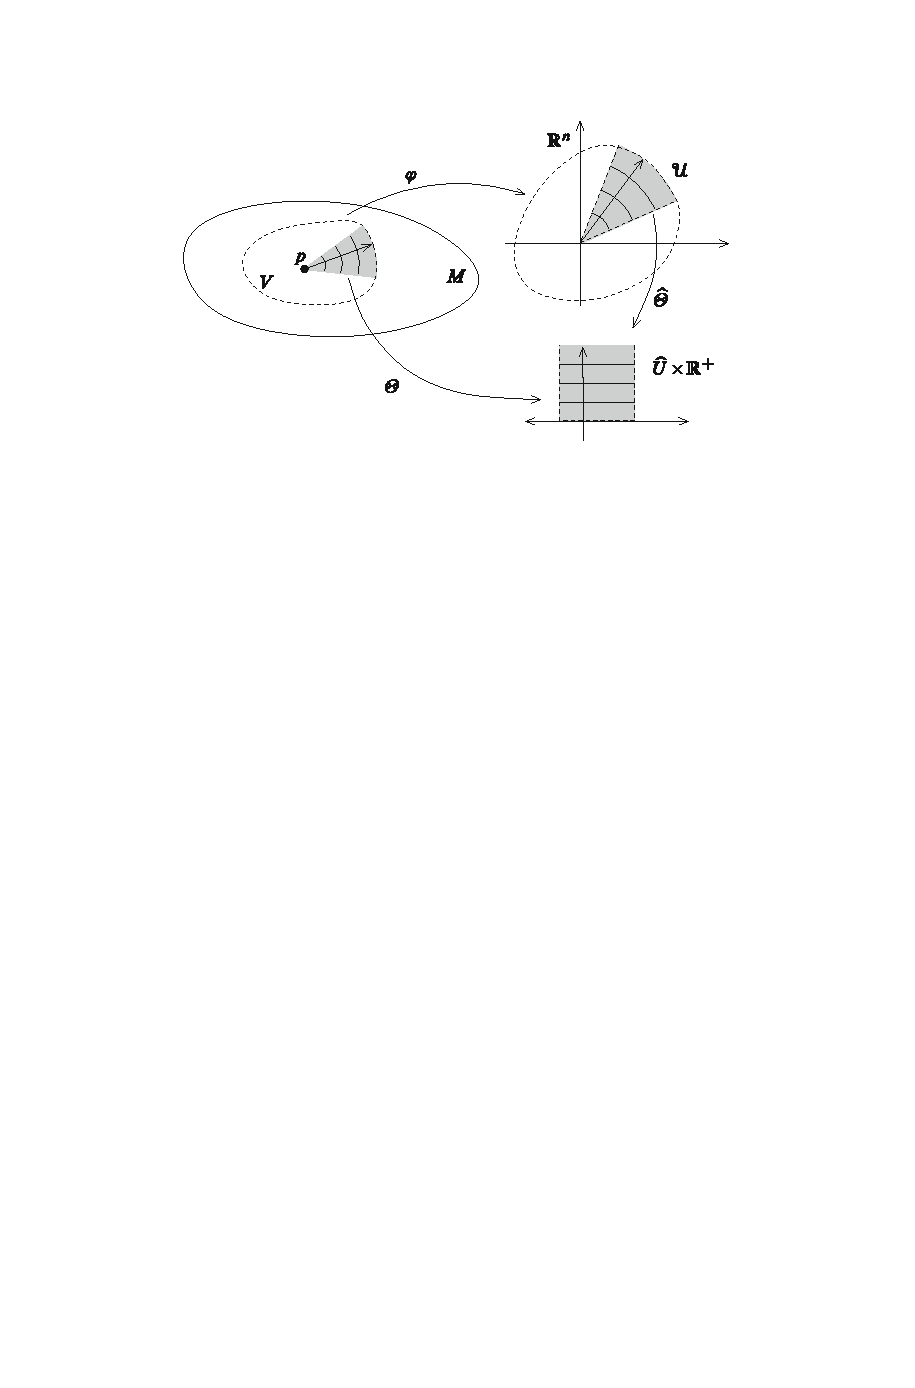
\includegraphics{pictures/polar-normal-coordinates}
\caption{Polar normal coordinates.}
\end{figure}

Now let $(M,g)$ be a Riemannian $n$-manifold, $p$ a point in $M$, and $\varphi$ any normal coordinate chart defined on a normal neighborhood $V$ of $p$. For every 
choice of polar coordinates $(\mathcal{U},\hat{\varTheta})$ for $\R^n\setminus\{0\}$, we obtain a smooth coordinate map $\varTheta=\hat{\varTheta}\circ\varphi$ on an open subset of $V\setminus\{p\}$. Such coordinates are called \textbf{polar normal coordinates}. They have the property that the last coordinate function $r$ is the radial distance function on $V$, and the other coordinates are constant along the integral curves of $\grad r$, so they are semigeodesic coordinates.
\item[(d)] \textbf{Polar Fermi Coordinates}. Now let $P$ be an embedded submanifold of $(M,g)$, and let $\varphi=(x^1,\dots,x^k,v^1,\dots,v^{n-k})$ be Fermi coordinates on a neighborhood $U_0$ of a point $p\in P$. Then any polar coordinate map $\hat{\varTheta}$ for $\R^{n-k}$ can be applied to the variables $(v^1,\dots,v^{n-k})$ to yield a coordinate chart $\varTheta=(\id_{\R^k}\times\hat{\varTheta})\circ\varphi$ on an open subset of $U_0\setminus P$, taking values in $\R^k\times\R^{n-k-1}\times\R^+$. If we write the coordinate functions as $(x^1,\dots,x^k,\theta^1,\dots,\theta^{n-k-1},r)$, it follows from Proposition~\ref{Riemann Fermi coordinate prop} that each coordinate curve $t\mapsto(x^1,\dots,x^k,\theta^1,\dots,\theta^{n-k-1},t)$ is a unit-speed geodesic. Thus these are semigeodesic coordinates, called \textbf{polar Fermi coordinates}. The polar normal coordinates described above are just the special case $P=\{p\}$.
\end{itemize}
\end{example}
\chapter{Curvature}
\section{The definition of curvature and basic properties}
\subsection{The curvature tensor}
Let $(M,g)$ be a Riemannian manifold and $\nabla$ the Riemannian connection. The curvature tensor is the $(1,3)$-tensor defined by (Proposition~\ref{connection second derivative})
\begin{align*}
R(X,Y)Z&=\nabla^2_{X,Y}Z-\nabla^2_{Y,X}Z\\
&=\nabla_X\nabla_YZ-\nabla_Y\nabla_XZ-\nabla_{[X,Y]}Z\\
&=[\nabla_X,\nabla_Y]Z-\nabla_{[X,Y]}Z
\end{align*}
on vector fields $X,Y,Z$. First let's verify that this indeed defines a tensor on $M$.
\begin{proposition}\label{Riemann curvature is tensor}
The map $R$ defined above is multilinear over $C^{\infty}(M)$, and thus defines a $(1,3)$-tensor field on $M$.
\end{proposition}
\begin{proof}
The map $R$ is obviously multilinear over $\R$. For $f\in C^{\infty}(M)$,
\begin{align*}
R(X,fY)Z&=\nabla_{X}\nabla_{fY}Z-\nabla_{fY}\nabla_{X}Z-\nabla_{[X,fY]}Z\\
&=\nabla_X(f\nabla_YZ)-f\nabla_Y\nabla_XZ-\nabla_{f[X,Y]+(Xf)Y}Z\\
&=(Xf)\nabla_YZ+f\nabla_X\nabla_YZ-f\nabla_Y\nabla_XZ-f\nabla_{[X,Y]}Z-(Xf)\nabla_{Y}Z\\
&=fR(X,Y)Z.
\end{align*}
The same proof shows that $R$ is linear over $C^\infty(M)$ in $X$, because $R(X,Y)=-R(Y,X)$ from the definition. For the variable $Z$, we first note that
\begin{align*}
\nabla^2_{X,Y}(fZ)&=\nabla_X\nabla_Y(fZ)-\nabla_{\nabla_XY}(fZ)\\
&=\nabla_X((Yf)Z+f\nabla_YZ)-\big((\nabla_XY)f\big)Z-f\nabla_{\nabla_XY}Z\\
&=(XYf)Z+(Yf)\nabla_XZ+(Xf)(\nabla_YZ)+f\nabla_{X}\nabla_YZ-\big((\nabla_XY)f\big)Z-f\nabla_{\nabla_XY}Z\\
&=\big(XYf-(\nabla_XY)f\big)Z+(Yf)\nabla_XZ+(Xf)(\nabla_YZ)+f\nabla_{X,Y}^2Z\\
&=(\nabla^2_{X,Y}f)Z+(Yf)\nabla_XZ+(Xf)(\nabla_YZ)+f\nabla_{X,Y}^2Z.
\end{align*}
Repalce the place of $X,Y$ and substrating, we get
\begin{align*}
&R(X,Y)(fZ)=\nabla_{X,Y}(fZ)-\nabla_{Y,X}(fZ)=(R_{X,Y}f)Z+fR(X,Y)Z=fR(X,Y)Z.
\end{align*}
where we use the fact that $R_{X,Y}f=0$ for $f\in C^\infty(M)$. This completes the proof.
\end{proof}
Thanks to this proposition, for each pair of vector fields $X,Y\in\X(M)$, the map $R_{X,Y}:\X(M)\to\X(M)$ given by $Z\mapsto R(X,Y)Z$ is a smooth bundle endomorphism of $TM$, called the \textbf{curvature endomorphism determined by $\bm{X}$ and $\bm{Y}$}. The tensor field $R$ itself is called the \textbf{(Riemann) curvature endomorphism} or the \textbf{$\bm{(1,3)}$-curvature tensor}.\par
The next proposition gives one reason for our interest in the curvature tensor.
\begin{proposition}
The curvature tensor is a local isometry invariant: if $(M,g)$ and $(\widetilde{M},\tilde{g})$ are (pseudo-)Riemannian manifolds and $\varphi:M\to\widetilde{M}$ is a local isometry, then $\varphi^*\tilde{R}=R$. More precisely,
\[\tilde{R}_{\varphi(p)}(d\varphi_p(X_p),d\varphi_p(Y_p))d\varphi_p(Z_p)=d\varphi_p(R_p(X_p,Y_p)Z_p)\]
for every $p\in M$ and $X,Y,Z\in\X(M)$.
\end{proposition}
\begin{proof}
This question is local, so we can assume that $\varphi$ is a isometry. In this case, the pull back connection $\varphi^*\widetilde{\nabla}$ is the Levi-civita connection on $M$ (Proposition~\ref{connection pull back}), therefore the claim follows. 
\end{proof}
As a $(1,3)$-tensor field, the curvature endomorphism can be written in terms of any local frame with one upper and three lower indices. We adopt the convention that the last index is the contravariant (upper) one. (This is contrary to our default assumption that covector arguments come first.) Thus, for example, the curvature endomorphism can be written in terms of local coordinates $(x^i)$ as
\[R=R_{ijk}^{l}dx^i\otimes dx^j\otimes dx^k\otimes\partial_l.\]
where the coefficients $R_{ijk}^l$ are defined by
\[R(\partial_i,\partial_j)\partial_k=R_{ijk}^l\partial_l.\]
The next proposition shows how to compute the components of $R$ in coordinates.
\begin{proposition}
Let $(M,g)$ be a (pseudo-)Riemannian manifold. In terms of any smooth local coordinates, the components of the $(1,3)$-curvature tensor are given by
\[R_{ijk}^l=\partial_i\Gamma_{jk}^l-\partial_j\Gamma_{ik}^l+\Gamma_{is}^l\Gamma_{jk}^s-\Gamma_{js}^l\Gamma_{ik}^s.\]
\end{proposition}
\begin{proof}
Note that
\begin{align*}
R(\partial_i,\partial_j)\partial_k&=\nabla_{\partial_i}\nabla_{\partial_j}\partial_k-\nabla_{\partial_j}\nabla_{\partial_i}\partial_k-\nabla_{[\partial_i,\partial_j]}\partial_k\\
&=\nabla_{\partial_i}(\Gamma_{jk}^s\partial_s)-\nabla_{\partial_j}(\Gamma_{ik}^s\partial_s)\\
&=\partial_i\Gamma_{jk}^s\partial_s+\Gamma_{jk}^s\nabla_{\partial_i}\partial_s-\partial_j\Gamma_{ik}^s\partial_s-\Gamma_{ik}^s\nabla_{\partial_j}\partial_s\\
&=\partial_i\Gamma_{jk}^s\partial_s+\Gamma_{jk}^s\Gamma_{is}^l\partial_l-\partial_j\Gamma_{ik}^s\partial_s-\Gamma_{ik}^s\Gamma_{js}^l\partial_l\\
&=(\partial_i\Gamma_{jk}^l-\partial_j\Gamma_{ik}^l+\Gamma_{is}^l\Gamma_{jk}^s-\Gamma_{js}^l\Gamma_{ik}^s)\partial_l
\end{align*}
therefore the claim follows.
\end{proof}
From the proof of Proposition~\ref{Riemann curvature is tensor}, we see that the curvature tensor acts trivially on functions. Now we want to extend this result. Recall that given vector fields $X$ and $Y$, we have the dual map $R_{X,Y}^*$ defined by
\[(R_{X,Y}^*\omega)(Z)=\omega(R_{X,Y}Z).\]
\begin{theorem}[\textbf{Ricci Identities}]
On a (pseudo-)Riemannian manifold $M$, the second total covariant derivatives of vector and tensor fields satisfy the following identities.
\begin{itemize}
\item[(a)] If $Z$ is a smooth vector field, then
\begin{align}\label{Riemann Ricci identity-1}
R_{X,Y}Z=(\nabla_{X,Y}^2-\nabla_{Y,X}^2)Z.
\end{align}
\item[(b)] If $\omega$ is a smooth $1$-form, then
\begin{align}\label{Riemann Ricci identity-2}
R_{X,Y}\omega=(\nabla_{X,Y}^2-\nabla_{Y,X}^2)\omega=-R_{X,Y}^*\omega
\end{align}
\item[(c)] If $F$ is a smooth $(r,s)$-tensor field, then
\begin{equation}\label{Riemann Ricci identity-3}
\begin{aligned}
&\quad R_{X,Y}F(\omega^1,\dots,\omega^r,V_1,\dots,V_s)=(\nabla_{X,Y}^2F-\nabla_{Y,X}^2F)(\omega^1,\dots,\omega^r,V_1,\dots,V_s)\\
&=\sum_{i=1}^rF(\omega^1,\dots,R_{X,Y}^*\omega^i,\dots,\omega^r,Y_1,\dots,Y_s)-\sum_{j=1}^sF(\omega^1,\dots,\omega^r,Y_1,\dots,R_{X,Y}Y_j,\dots,Y_s).
\end{aligned}
\end{equation}
\end{itemize}
\end{theorem}
\begin{proof}
We first prove $(\ref{Riemann Ricci identity-2})$. Using $(\ref{connection second derivative})$ repeatedly, we compute
\begin{align*}
(\nabla_X\nabla_Y\omega)(Z)&=X((\nabla_Y\omega)(Z))-(\nabla_Y\omega)(\nabla_XZ)\\
&=X\big(Y(\omega(Z))-\omega(\nabla_YZ)\big)-(\nabla_Y\omega)(\nabla_XZ)\\
&=XY(\omega(Z))-\omega(\nabla_X\nabla_YZ)-(\nabla_X\omega)(\nabla_YZ)-(\nabla_Y\omega)(\nabla_XZ).
\end{align*}
Reversing the roles of $X$ and $Y$, we get
\begin{align*}
(\nabla_X\nabla_Y\omega)(Z)=YX(\omega(Z))-\omega(\nabla_Y\nabla_XZ)-(\nabla_Y\omega)(\nabla_XZ)-(\nabla_X\omega)(\nabla_YZ).
\end{align*}
and applying $(\ref{connection second derivative})$ once more yields
\[(\nabla_{[X,Y]}\omega)(Z)=[X,Y](\omega(Z))-\omega(\nabla_{[X,Y]}Z).\]
Therefore
\begin{align*}
(\nabla_{X}\nabla_Y\omega-\nabla_Y\nabla_X\omega-\nabla_{[X,Y]}\omega)(Z)&=-\omega(\nabla_X\nabla_YZ-\nabla_{Y}\nabla_XZ)+\omega(\nabla_{[X,Y]}Z)\\
&=-\omega(R_{X,Y}Z)=-(R_{X,Y}^*\omega)(Z).
\end{align*}
Next consider the action of $R_{X,Y}$ on an arbitrary tensor product: (see the calculation in Proposition~\ref{Riemann curvature is tensor})
\begin{align*}
\nabla^2_{X,Y}(F\otimes G)&=(\nabla_X\nabla_Y-\nabla_{\nabla_XY})(F\otimes G)\\
&=(\nabla_{X,Y}^2F)\otimes G+(\nabla_YF)\otimes(\nabla_XG)+(\nabla_XF)\otimes(\nabla_YG)+F\otimes\nabla_{X,Y}^2G.
\end{align*}
Therefore
\begin{equation*}
\begin{aligned}
R_{X,Y}(F\otimes G)=(\nabla_{X,Y}^2-\nabla_{Y,X}^2)(F\otimes G)=\big((\nabla_{X,Y}^2-\nabla_{Y,X})F\big)\otimes G+F\otimes\big((\nabla_{X,Y}^2-\nabla_{Y,X}^2)G\big).
\end{aligned}
\end{equation*}
A simple induction using this relation together with $(\ref{Riemann Ricci identity-1})$ and $(\ref{Riemann Ricci identity-2})$ gives $(\ref{Riemann Ricci identity-3})$.
\end{proof}
For many purposes, the information contained in the curvature endomorphism is much more conveniently encoded in the form of a covariant $4$-tensor. We define the 
(Riemann) curvature tensor to be the $(0,4)$-tensor field
\[R(X,Y,Z,W)=\langle R(X,Y)Z,W\rangle.\]
In terms of any smooth local coordinates it is written
\[R=R_{ijkl}dx^i\otimes dx^j\otimes dx^k\otimes dx^l.\]
where $R_{ijkl}=R_{ijk}^sg_{sl}$. We justify next why the variables are treated on a more equal footing in this formula by showing several important symmetry properties.
\begin{proposition}[\textbf{Symmetries of the Curvature Tensor}]\label{Riemann curvature symmetry}
The curvature tensor $R(X,Y,Z,W)$ satisfies the following properties:
\begin{itemize}
\item[(a)] $R$ is skew-symmetric in the first two and last two entries:
\[R(X,Y,Z,W)=-R(Y,X,Z,W),\quad R(X,Y,Z,W)=-R(X,Y,W,Z).\] 
\item[(b)] $R$ is symmetric between the first two and last two entries:
\[R(X,Y,Z,W)=R(Z,W,X,Y).\] 
\item[(c)] $R$ satisfies a cyclic permutation property called \textbf{algebraic Bianchi identity}:
\[R(X,Y)Z+R(Y,Z)X+R(Z,X)Y=0.\] 
\end{itemize}
\end{proposition}
\begin{proof}
The first part of (a) has already been established. For part two of (a) we compute
\begin{align*}
R(X,Y,Z,Z)&=\langle\nabla_X\nabla_YZ,Z\rangle-\langle\nabla_Y\nabla_XZ,Z\rangle-\langle\nabla_{[X,Y]}Z,Z\rangle\\
&=\nabla_X\langle\nabla_YZ,Z\rangle-\langle\nabla_YZ,\nabla_XZ\rangle-\nabla_Y\langle\nabla_XZ,Z\rangle\\
&\ +\langle\nabla_XZ,\nabla_YZ\rangle-\langle\nabla_{[X,Y]}Z,Z\rangle\\
&=\nabla_X\langle\nabla_YZ,Z)-\nabla_Y\langle\nabla_XZ,Z)-\langle\nabla_{[X,Y]}Z,Z)\\
&=\frac{1}{2}\big(\nabla_X\nabla_Y\langle Z,Z\rangle-\nabla_Y\nabla_X\langle Z,Z\rangle-\nabla_{[X,Y]}\langle Z,Z\rangle\big)\\
&=\frac{1}{2}R_{X,Y}\langle Z,Z\rangle=0.
\end{align*}
Now (a) follows by polarizing the identity $R(X,Y,Z,Z)$ in $Z$:
\[0=R(X,Y,Z+W,Z+W)=R(X,Y,Z,W)+R(X,Y,W,Z).\]
Part (c) relies on the torsion free property and the definition of $R$ and the symmetry of the connection:
\begin{align*}
&R(X,Y)Z+R(Y,Z)X+R(Z,X)Y\\
&=(\nabla_X\nabla_YZ-\nabla_Y\nabla_XZ-\nabla_{[X,Y]}Z)+(\nabla_Y\nabla_ZX-\nabla_Z\nabla_YX-\nabla_{[Y,Z]}X)\\
&\quad+(\nabla_Z\nabla_XY-\nabla_X\nabla_ZY-\nabla_{[Z,X]}Y)\\
&=\nabla_X(\nabla_YZ-\nabla_ZY)+\nabla_Y(\nabla_ZX-\nabla_XZ)+\nabla_Z(\nabla_XY-\nabla_YX)\\
&\quad-\nabla_{[X,Y]}Z-\nabla_{[Y,Z]}X-\nabla_{[Z,X]}Y\\
&=\nabla_X[Y,Z]+\nabla_Y[Z,X]+\nabla_Z[X,Y]-\nabla_{[X,Y]}Z-\nabla_{[Y,Z]}X-\nabla_{[Z,X]}Y\\
&=[X,[Y,Z]]+[Y,[Z,X]]+[Z,[X,Y]]\\
&=0.
\end{align*}
Now we show that identity (b) follows from (a) and (c). Writing the algebraic Bianchi identity four times with indices cyclically permuted gives
\begin{align*}
R(X,Y,Z,W)+R(Y,Z,X,W)+R(Z,X,Y,W)&=0,\\
R(Y,Z,W,X)+R(Z,W,Y,X)+R(W,Y,Z,X)&=0,\\
R(Z,W,X,Y)+R(W,X,Z,Y)+R(X,Z,W,Y)&=0,\\
R(W,X,Y,Z)+R(X,Y,W,Z)+R(Y,W,X,Z)&=0.
\end{align*}
Now add up all four equations. Applying (a) four times makes all the terms in the first two columns cancel. Then applying (a) in the last column yields
\[2R(Z,X,Y,W)+2R(W,Y,Z,X)=0,\]
which is equivalent to (b).
\end{proof}
\begin{proposition}[\textbf{Differential Bianchi Identity}]\label{Riemann differential Bianchi}
The total covariant derivative of the curvature tensor satisfies the following identity:
\[(\nabla_ZR)(X,Y)W+(\nabla_XR)(Y,Z)W+(\nabla_{Y}R)(Z,X)W=0.\]
\end{proposition}
\begin{proof}
We first give an equation about $(\nabla_Z)R(X,Y)W$. Using Proposition~\ref{connection def on tensor}, we find that
\begin{equation*}
\begin{aligned}
(\nabla_ZR^{\flat})&(X,Y,W,V)=X\langle R(X,Y)W,V\rangle\\
&-R(\nabla_ZX,Y,W,V)-R(X,\nabla_ZY,W,V)-R(X,Y,\nabla_ZW,V)-R(X,Y,W,\nabla_ZV).
\end{aligned}
\end{equation*}
Therefore, by the metric compactibility,
\begin{equation*}
\begin{aligned}
&\langle\nabla_Z(R(X,Y)W),V\rangle=X\langle R(X,Y)W,V\rangle-\langle R(X,Y)W,\nabla_ZV\rangle\\
&=(\nabla_ZR^{\flat})(X,Y,W,V)+R(\nabla_ZX,Y,W,V)+R(X,\nabla_ZY,W,V)+R(X,Y,\nabla_ZW,V)\\
&=(\nabla_ZR)^{\flat}(X,Y,W,V)+R(\nabla_ZX,Y,W,V)+R(X,\nabla_ZY,W,V)+R(X,Y,\nabla_ZW,V)\\
&=\langle(\nabla_ZR)(X,Y)W,V\rangle+R(\nabla_ZX,Y,W,V)+R(X,\nabla_ZY,W,V)+R(X,Y,\nabla_ZW,V).
\end{aligned}
\end{equation*}
where we use the fact $(\nabla R)^\flat=\nabla(R^\flat)$ (Proposition~\ref{connection total derivative flat sharp}). Then since $V$ is arbitrary, we conclude that
\begin{equation}\label{Riemann differential Bianchi-1}
\begin{aligned}
&\nabla_Z(R(X,Y)W)=(\nabla_ZR)(X,Y)W+R(\nabla_ZX,Y)W+R(X,\nabla_ZY)W+R(X,Y)\nabla_ZW,\\
&\nabla_X(R(Y,Z)W)=(\nabla_XR)(Y,Z)W+R(\nabla_XY,Z)W+R(Y,\nabla_XZ)W+R(Y,Z)\nabla_XW,\\
&\nabla_Y(R(Z,X)W)=(\nabla_YR)(Z,X)W+R(\nabla_YZ,X)W+R(Z,\nabla_YX)W+R(Z,X)\nabla_YW.
\end{aligned}
\end{equation}
Recall that $R(X,Y)=-R(Y,X)$, so adding the third and fourth columns of $(\ref{Riemann differential Bianchi-1})$ yeilds
\begin{align*}
&\text{The sum of the third and fourth columns of $(\ref{Riemann differential Bianchi-1})$}\\
&=R(\nabla_YZ-\nabla_ZY,X)W+R(\nabla_XY-\nabla_YX,Z)W+R(\nabla_YZ-\nabla_ZY,X)\\
&=R([Y,Z],X)W+R([X,Y],Z)W+R([Y,Z],X)W.
\end{align*}
Also, adding the left side of $(\ref{Riemann differential Bianchi-1})$ gives
\begin{align*}
&\nabla_Z(R(X,Y)W)+\nabla_X(R(Y,Z)W)+\nabla_Y(R(Z,X)W)\\
&=(\nabla_Z\nabla_X\nabla_YW-\nabla_Z\nabla_Y\nabla_XW-\nabla_Z\nabla_{[X,Y]}W)\\
&\quad +(\nabla_X\nabla_Y\nabla_ZW-\nabla_X\nabla_Z\nabla_YW-\nabla_X\nabla_{[Y,Z]}W)\\
&\quad +(\nabla_Y\nabla_Z\nabla_XW-\nabla_Y\nabla_X\nabla_ZW-\nabla_Y\nabla_{[Z,X]}W)\\
&=(\nabla_X\nabla_Y-\nabla_Y\nabla_X)\nabla_ZW-\nabla_Z\nabla_{[X,Y]}W\\
&\quad +(\nabla_Y\nabla_Z-\nabla_Z\nabla_Y)\nabla_XW-\nabla_X\nabla_{[Y,Z]}W\\
&\quad +(\nabla_Z\nabla_X-\nabla_X\nabla_Z)\nabla_YW-\nabla_Y\nabla_{[Z,X]}W\\
&=\nabla_{[X,Y]}\nabla_ZW-\nabla_Z\nabla_{[X,Y]}W+R(X,Y)\nabla_ZW\\
&\quad +\nabla_{[Y,Z]}\nabla_XW-\nabla_X\nabla_{[Y,Z]}W+R(Y,Z)\nabla_XW\\
&\quad +\nabla_{[Z,X]}\nabla_YW-\nabla_Y\nabla_{[Z,X]}W+R(Z,X)\nabla_YW\\
&=\nabla_{[[X,Y],Z]}W+R([X,Y],Z)W+R(X,Y)\nabla_ZW\\
&\quad +\nabla_{[[Y,Z],X]}W+R([Y,Z],X)W+R(Y,Z)\nabla_XW\\
&\quad +\nabla_{[[Z,X],Y]}W+R([Z,X],Y)W+R(Z,X)\nabla_YW\\
&=R([X,Y],Z)W+R([Y,Z],X)W+R([Z,X],Y)W\\
&\quad +R(X,Y)\nabla_ZW+R(Y,Z)\nabla_XW+R(Z,X)\nabla_YW.
\end{align*}
Now adding $(\ref{Riemann differential Bianchi-1})$ together and apply the established equalities, we finally get
\[(\nabla_ZR)(X,Y)W+(\nabla_XR)(Y,Z)W+(\nabla_YR)(Z,X)W=0.\]
This completes the proof.
\end{proof}
\begin{corollary}
The covariant derivative of the curvature tensor $R(X,Y,V,W)$ satisfies the following differential Bianchi identity:
\[(\nabla R)(X,Y,V,W,Z)+(\nabla R)(X,Y,W,Z,V)+(\nabla R)(X,Y,Z,V,W)=0.\]
In components, this is
\begin{align}\label{Riemann differential Bianchi (0,4)}
R_{ijkl;s}+R_{ijls;k}+R_{ijsk;l}=0.
\end{align}
\end{corollary}
\begin{proof}
Since $(\nabla R)^\flat=\nabla(R^\flat)$, by the differential Bianchi identity of $R(X,Y)Z$ we have
\[(\nabla_ZR)(V,W,X,Y)+(\nabla_VR)(W,Z,X,Y)+(\nabla_WR)(Z,V,X,Y)=0.\]
Using the symmetric property of $R(X,Y,V,W)$, we get the claim.
\end{proof}
\begin{remark}
Since the $(0,4)$-tensor $R(X,Y,V,W)$ is used more frequently, without further remark, we will use $R$ to denote this tensor. Then $(1,3)$ curvature tensor will be 
denote by $R(X,Y)Z$, typically.
\end{remark}
\subsection{Curvature and differential forms}
Since the curvature operator involves the second derivative and the christoffel symbol, it is often hard to compute it. Now we use differentiable forms to give an 
computational accessible expression of the curvature of a Riemannian manifold.\par
Let $M$ be a smooth $n$-manifold and $\nabla$ a connection in $TM$, let $(E_i)$ be a local frame on some open subset $U\sub M$, and let $(\eps^i)$ be the dual coframe. 
Let $X\in\X(M)$, then the connection $\nabla_XE_i$ can written into a linear combination of $E_j$:
\[\nabla_XE_i=\omega_i^j(X)E_j.\]
The $n\times n$ matrix of smooth $1$-forms $(\omega_i^j)$ on $U$ is then uniquely determined by the connection $\nabla$ and $(E_i)$, and is called the 
\textbf{connection $\bm{1}$-forms} for this frame.\par
Similarly, for $X,Y\in\X(M)$, the vector field $R(X,Y)E_i$ is a linear combination of $(E_j)$:
\[R(X,Y)E_i=\Omega_i^j(X,Y)E_j.\]
The $n\times n$ matrix of smooth $2$-forms $(\Omega_i^j)$ is called the \textbf{curvature $2$-forms} for this frame.
\begin{proposition}
The connection form and the curvature form are given by
\[\omega_i^j(X)=\Gamma_{ki}^j\eps^k,\quad \Omega_i^j=\frac{1}{2}R_{kli}^j\,\eps^k\wedge\eps^l,\]
where $(\eps^j)$ is the coframe dual to $(E_i)$.
\end{proposition}
\begin{proof}
Write $X=X^kE_k$, then
\[\nabla_XE_i=X_k\nabla_{E_k}E_i=X^k\Gamma_{ki}^jE_j.\]
Therefore $\omega_i^j(X)=\Gamma_{ki}^jX^k$, that is, $\omega_i^j=\Gamma_{ki}^j\eps^k$. Similarly, we have
\begin{align*}
R(X,Y)E_i&=X^kY^lR(E_k,E_l)E_i=X^{k}Y^lR_{kli}^jE_j.
\end{align*}
Since $R(X,Y)$ is antisymmetric, we find 
\begin{align*}
(R_{kli}^j\eps^k\wedge\eps^l)(X,Y)&=R_{kli}^j(X^kY^l-Y^kX^l)=R_{kli}^jX^kY^l-R_{kli}^jY^kX^l=2R_{kli}^jX^kY^l.
\end{align*}
Therefore we get the second equation.
\end{proof}
For $X,Y\in\X(M)$, the torsion $\tau(X,Y)$ is a smooth $2$-tensor, so we can write $\tau(X,Y)=\tau^i(X,Y)E_i$ for some $2$-forms on $M$, called the \textbf{torsion forms} of the 
connection $\nabla$.
\begin{proposition}
Let $\omega$ and $\Omega$ be the connection and curvature forms, then we have the following structural equations:
\begin{itemize}
\item[(\rmnum{1})] (\textbf{Cartan's first sturcture equation})
\begin{align}\label{Riemann sturcture equation-1}
d\eps^j=\eps^i\wedge\omega_i^j+\tau^j.
\end{align}
\item[(\rmnum{2})] (\textbf{Cartan's second sturcture equation})
\begin{align}\label{Riemann sturcture equation-2}
d\omega_i^j=\omega_i^k\wedge\omega_k^j+\Omega_i^j.
\end{align}
\end{itemize}
\end{proposition}
\begin{proof}
For (\rmnum{1}), by the definition of $\omega_i^j$, we have
\begin{align*}
\nabla_XY&=\nabla_X(Y^iE_i)=\nabla_X(\eps^i(Y)E_i)\\
&=X(\eps^i(Y))E_i+\eps^i(Y)\nabla_XE_i\\
&=X(\eps^j(Y))E_j+\eps^i(Y)\omega_i^j(X)E_j.
\end{align*}
Interchanging $X$ and $Y$, we get $\nabla_YX=Y(\eps^j(Y))E_j+\eps^i(X)\omega_i^j(Y)E_j$, and therefore 
\begin{align*}
\tau(X,Y)&=\big(X(\eps^j(Y))-Y(\eps^j(X))-\eps^j([X,Y])\big)E_i+\big(\eps^i(Y)\omega_i^j(X)-\eps^i(X)\omega_i^j(Y)\big)E_j\\
&=d\eps^j(X,Y)E_j-(\eps^i\wedge\omega_i^j)(X,Y)E_j.
\end{align*}
This gives $\tau^j=d\eps^j-\eps^i\wedge\omega_i^j$, which is (\rmnum{1}).\par
For (\rmnum{2}), note that
\begin{align*}
\nabla_X\nabla_YE_i&=\nabla_X(\omega_i^k(Y)E_k)\\
&=X(\omega_i^k(Y))E_k+\omega_i^k(Y)\nabla_XE_k\\
&=X(\omega_i^j(Y))E_j+\omega_i^k(Y)\omega_k^j(X)E_j
\end{align*}
Interchanging $X$ and $Y$, we get $\nabla_Y\nabla_XE_i=Y(\omega_i^j(X))E_j+\omega_i^k(Y)\omega_k^j(Y)E_j$. Furthermore,
\[\nabla_{[X,Y]}E_i=\omega_i^j([X,Y])E_j.\]
Therefore,
\begin{align*}
R(X,Y)E_i&=\big(X(\omega_i^j(Y))-Y(\omega_i^j(X))-\omega_i^j([X,Y])\big)E_j+\big(\omega_i^k(Y)\omega_k^j(X)-\omega_i^k(X)\omega_k^j(Y)\big)E_j\\
&=d\omega_i^j(X,Y)E_j-(\omega_i^k\wedge\omega_k^j)(X,Y)E_j.
\end{align*}
Comparing this with the definition of the curvature form $\Omega_i^j$ gives (\rmnum{2}).
\end{proof}
\begin{corollary}
Let $(M,g)$ be a Riemannian manifold and $\nabla$ be its Levi-Civita connection, then the structural equations of $\nabla$ are
\begin{align}\label{Riemann Levi-Civita sturcture equation}
d\eps^j=\eps^i\wedge\omega_i^j,\quad d\omega_i^j=\Omega_i^j+\omega_i^k\wedge\omega_k^j.
\end{align}
\end{corollary}
\begin{proof}
Recall that the Levi-Civita connection is torsion-free.
\end{proof}
If $A=[\alpha_i^j]$ and $B=[\beta_i^j]$ are matrices of differential forms on $M$ with the number of columns of $A$ equal to the number of rows of $B$, then their wedge 
product $A\wedge B$ is defined to be the matrix of differential forms whose $(i,j)$-entry is
\[(A\wedge B)_i^j=\alpha_i^k\wedge\beta_k^j\]
and $dA$ is defined to be $[d\alpha_i^j]$. In matrix notation, we write
\[\tau=\begin{bmatrix}
\tau^1\\
\vdots\\
\tau^n
\end{bmatrix}\quad \eps=\begin{bmatrix}
\eps^1\\
\vdots\\
\eps^n
\end{bmatrix}\quad \omega=[\omega_i^j]\quad \Omega=[\Omega_i^j].\]
Then the structural equations can be written as
\[d\eps=\eps\wedge\omega+\tau,\quad d\omega=\omega\wedge\omega+\Omega.\]
Apart from the structural equations, we now explore more properties of the connection and curvature forms.
\begin{proposition}
Let $(M,g)$ be a Riemannian manifold and $\nabla$ a connection on $TM$.
\begin{itemize}
\item[(a)] If the connection $\nabla$ is compatible with the metric, then its connection matrix $[\omega_i^j]$ relative to any local orthonormal frame $(E_i)$ over an 
open set $U\sub M$ is skew-symmetric.
\item[(b)] If every point $p\in M$ has a local orthonormal frame on a neighborhood $U\sub M$ such that the connection matrix $[\omega_i^j]$ relative to $(E_i)$ is 
skew-symmetric, then the connection $\nabla$ is compatible with the metric.
\end{itemize}
\end{proposition}
\begin{proof}
Part (a) is straightforward, just note that
\[0=X\langle E_i,E_j\rangle=\langle\nabla_XE_i,E_j\rangle+\langle E_i,\nabla_XE_j\rangle=\omega_i^j+\omega_j^i.\]
For part (b), we note first that compatibility with the metric is a local condition, so $\nabla$ is compatible with the metric if and only if its restriction $\nabla^U$ 
to any open set $U$ is compatible with the metric. Suppose $\omega_i^j=-\omega_j^i$. Let $Y=X^iE_i$ and $Z=Z^jE_j$, with $Y^i,Z^j\in C^{\infty}(U)$. Then
\begin{align*}
\nabla_XY&=\nabla_X(Y^iE_i)=X(Y^i)E_i+Y^i\omega_i^j(X)E_j,\\
\nabla_XZ&=\nabla_X(Z^jE_j)=X(Z^j)E_j+Z^j\omega_j^i(X)E_i.
\end{align*}
Therefore 
\begin{align*}
\langle\nabla_XY,Z\rangle&=\sum_iX(Y^i)Z^i+Y^iZ^j\omega_i^j(X),\\
\langle Y,\nabla_XZ\rangle&=\sum_jX(Z^j)Y^j+Y^iZ^j\omega_j^i(X).
\end{align*}
Since $\omega_i^j+\omega_j^i=0$, we then find
\begin{align*}
\langle\nabla_XY,Z\rangle+\langle Y,\nabla_XZ\rangle&=\sum_iX(Y^i)Z^i+\sum_jX(Z^j)Y^j=X\langle Y,Z\rangle.
\end{align*}
Therefore $\nabla$ is a metric connection.
\end{proof}
\begin{proposition}
If the connection matrix $[\omega_i^j]$ relative to a local frame $(E_i)$ of an connection is skew-symmetric, then so is the curvature matrix $[\Omega_i^j]$.
\end{proposition}
\begin{proof}
By the structural equation,
\[\Omega_i^j=d\omega_i^j-\omega_i^k\wedge\omega_k^j=-d\omega_j^i-\omega_k^i\wedge\omega^k_j=-(d\omega_j^i-\omega_j^k\wedge\omega_k^i)=-\Omega_j^i.\]
Therefore $[\Omega_i^j]$ is also skew-symmetric.
\end{proof}
\begin{example}
As a special case, if $n=2$ and $(E_1,E_2)$ is a local orthonormal frame for $M$ with dual frame $(\eps^1,\eps^2)$, then $[\omega_i^j]$ and $[\Omega_i^j]$ are both skew-symmetric, and in particular the curvature forms of $M$ reduce to the $2$-form $\Omega_1^2$. Moreover, by the structural equation $(\ref{Riemann sturcture equation-2})$, we have
\[\Omega_1^2=d\omega_1^2-\omega_1^1\wedge\omega_1^2-\omega_1^2\wedge\omega_2^2=d\omega_1^2.\]
Also, by the structural equation $(\ref{Riemann sturcture equation-2})$, $\omega_1^2$ can be computed by
\[d\eps^1=\eps^2\wedge\omega_2^1=-\eps^2\wedge\omega_1^2,\quad d\eps^2=\eps^1\wedge\omega_1^2.\]
Since $\eps^1\wedge\eps^2$ is a basis for $\Omega^2(M)$, from these two equalities we can solve $\omega_1^2$, and then get $\Omega_1^2$.
\end{example}
\begin{example}
The Poincar\'e disk is the open unit disk $\mathbb{D}$ in the complex plane with Riemannian metric
\[g=4\frac{dx^2+dy^2}{(1-|z|^2)^2}=4\frac{dx^2+dy^2}{(1-x^2-y^2)^2}.\]
An orthonormal frame for $\mathbb{D}$ is
\[E_1=\frac{1}{2}(1-|z|^2)\frac{\partial}{\partial x},\quad E_2=\frac{1}{2}(1-|z|^2)\frac{\partial}{\partial y},\]
with dual frames
\[\eps^1=\frac{2}{1-|z|^2}dx,\quad \eps^2=\frac{2}{1-|z|^2}dy.\]
Now we find the connection form $\omega_i^j$ for this frame. First we have
\[d\eps^1=-\frac{4y}{(1-|z|^2)^2}dx\wedge dy,\quad d\eps^2=\frac{4x}{(1-|z|^2)^2}dx\wedge dy.\]
Therefore by $(\ref{Riemann sturcture equation-1})$ and the relation $\omega_1^2=-\omega_2^1$ we then get
\[\omega_1^2=\frac{2x}{1-|z|^2}dy-\frac{2y}{1-|z|^2}dx.\]
With this, we then use $(\ref{Riemann sturcture equation-2})$ to compute $\Omega_1^2$:
\[\Omega_1^2=d\omega_1^2=\frac{4}{(1-|z|^2)^2}dx\wedge dy.\]
\end{example}
\begin{example}
Let $\mathbb{H}$ be the Poincar\'e half-plane wohse metric is given by
\[g=\frac{dx^2+dy^2}{y^2}.\]
With this metric, an orthonormal frame is
\[E_1=y\frac{\partial}{\partial y},\quad E_2=y\frac{\partial}{\partial y}\]
with dual frames
\[\eps^1=\frac{1}{y}dx,\quad \eps^2=\frac{1}{y}dy.\]
Then we have
\[d\eps^1=\frac{1}{y^2}dx\wedge dy,\quad d\eps^2=0,\]
and therefore $\omega_1^2=\frac{1}{y}dx$. With this, the curvature form is given by
\[\Omega_1^2=d\omega_1^2=\frac{1}{y^2}dx\wedge dy.\]
\end{example}
\begin{example}
Even more general, let $M$ be a two-dimensional Riemannian manifold that is locally conformally flat. Then there are local charts $(x,y)$ at each point of $M$ such that
\[g=f(x)(dx^2+dy^2)\]
under the local frames $(\partial/\partial x,\partial/\partial y)$, where $f$ is a smooth function. Since $f$ is then positive, the vector frames
\[E_1=\frac{1}{\sqrt{f}}\frac{\partial}{\partial x},\quad E_2=\frac{1}{\sqrt{f}}\frac{\partial}{\partial y}\]
are then orthonormal. The corresponding dual frames are $\eps^1=\sqrt{f}dx,\eps^2=\sqrt{f}dy$, so we have
\[d\eps^1=-\frac{f_y}{2\sqrt{f}}dx\wedge dy,\quad d\eps^2=\frac{f_x}{2\sqrt{f}}dx\wedge dy.\]
This then implies
\[\omega_1^2=-\frac{f_y}{2f}dx+\frac{f_x}{2f}dy,\quad \Omega_1^2=\frac{f(f_{xx}+f_{yy})-f_x^2-f_y^2}{2f^2}dx\wedge dy.\]
\end{example}
\begin{example}
If we parametrize $S^2$ by
\[(x,y,z)=(\cos\theta\sin\phi,\sin\theta\sin\phi,\cos\phi)\]
Then the metric is given by
\[g=\sin^2\phi\,d\theta^2+d\phi^2.\]
Therefore an orthonormal frame is given by $(1/\sin\phi)\partial_\theta,\partial_\phi$ with dual frames $(\sin\phi\,d\theta,d\phi)$. We compute that
\[d(\sin\phi\,d\theta)=-\cos\phi\,d\theta\wedge d\phi,\quad d(d\phi)=0.\] 
Therefore the connection form and the curvature form are given by
\[\omega_1^2=-\cos\phi\,d\theta,\quad\Omega_1^2=-\sin\phi\,d\theta\wedge d\phi.\]
\end{example}
\subsection{Flat manifolds}
Recall that the curvature operator endodes the failure of the exchange of covariant derivatives. Importantly for our purposes, we show that it also measures the failure of second covariant derivatives along families of curves to commute. Given a smooth one-parameter family of curves $\Gamma:J\times I\to M$, recall that the velocity fields $\partial_t\Gamma(s,t)=(\Gamma_s)'(t)$ and $\partial_s\Gamma(s,t)=(\Gamma^t)'(s)$ are smooth vector fields along $\Gamma$.
\begin{proposition}\label{Riemann curvature second derivatire curve}
Suppose $(M,g)$ is a smooth (pseudo-)Riemannian manifold and $\Gamma:J\times I\to M$ is a smooth one-parameter family of curves in $M$. Then for every smooth vector field $V$ along $\gamma$,
\begin{align}\label{Riemann curvature second derivatire curve-1}
D_sD_tV-D_tD_sV=R(\partial_s\Gamma,\partial_t\Gamma)V.
\end{align}
\end{proposition}
\begin{proof}
This is a local question, so for each $(s,t)\in J\times I$, we can choose smooth coordinates $(x^i)$ defined on a neighborhood of $\Gamma(s,t)$ and write
\[\Gamma(s,t)=(\gamma^1(s,t),\dots,\gamma^n(s,t))\quad V(s,t)=V^i(s,t)\partial_i|_{\Gamma(s,t)}.\]
Formula $(\ref{connection derivative curve-1})$ yields
\[D_tV=\frac{\partial V^i}{\partial t}\partial_i+V^iD_t\partial_i.\]
Therefore, applying $(\ref{connection derivative curve-1})$ again, we get
\[D_sD_tV=\frac{\partial^2V^i}{\partial s\partial t}\partial_i+\frac{\partial V^i}{\partial t}D_s\partial_i+\frac{\partial V^i}{\partial s}D_t\partial_i+V^iD_sD_t\partial_i.\]
Interchanging $s$ and $t$ and subtracting, we see that all the terms except the last cancel:
\begin{align}\label{Riemann curvature second derivatire curve-2}
D_sD_tV-D_tD_sV=V^i(D_sD_t\partial_i-D_tD_s\partial_i)
\end{align}
Now we need to compute the commutator in parentheses. Because $\partial_i$ is extendible,
\[D_t\partial_i=\nabla_{\partial_i\Gamma}\partial_i=\frac{\partial\gamma^j}{\partial t}\nabla_{\partial_j}\partial_i.\]
and therefore, because $\nabla_{\partial_j}\partial_i$ is also extendible,
\begin{align*}
D_sD_t\partial_i&=D_s\Big(\frac{\partial\gamma^j}{\partial t}\nabla_{\partial_j}\partial_i\Big)=\frac{\partial^2\gamma^j}{\partial s\partial t}\nabla_{\partial_j}\partial_i+\frac{\partial\gamma^j}{\partial t}\nabla_{\partial_s\Gamma}(\nabla_{\partial_j}\partial_i)\\
&=\frac{\partial^2\gamma^j}{\partial s\partial t}\nabla_{\partial_j}\partial_i+\frac{\partial\gamma^j}{\partial t}\frac{\partial\gamma^k}{\partial s}\nabla_{\partial_k}\nabla_{\partial_j}\partial_i.
\end{align*}
Interchanging $s\leftrightarrow t$ and $j\leftrightarrow k$ and subtracting, we find that the first terms cancel, and we get
\begin{align*}
D_sD_t\partial_i-D_tD_s\partial_i&=\frac{\partial\gamma^j}{\partial t}\frac{\partial\gamma^k}{\partial s}(\nabla_{\partial_k}\nabla_{\partial_j}\partial_i-\nabla_{\partial_j}\nabla_{\partial_k}\partial_i)\\
&=\frac{\partial\gamma^j}{\partial t}\frac{\partial\gamma^k}{\partial s}R(\partial_k,\partial_j)\partial_i\\
&=R(\partial_s\Gamma,\partial_t\Gamma)\partial_i.
\end{align*}
Finally, inserting this into $(\ref{Riemann curvature second derivatire curve-2})$ yields the result.
\end{proof}
Recall that a Riemannian manifold is said to be \textbf{flat} if it is locally isometric to a Euclidean space, that is, if every point has a neighborhood that is 
isometric to an open set in Rn with its Euclidean metric. Similarly, a pseudo-Riemannian manifold is flat if it is locally isometric to a pseudo-Euclidean space. 
We say that a connection $\nabla$ on a smooth manifold M satisfies the flatness criterion if whenever $X,Y,Z$ are smooth vector fields defined on an open subset of 
$M$, the following identity holds:
\begin{align}\label{Riemann flat crition}
\nabla_X\nabla_Y-\nabla_Y\nabla_X=\nabla_{[X,Y]}.
\end{align}
\begin{proposition}
 If $(M,g)$ is a flat (pseudo-)Riemannian manifold, then its Levi-Civita connection satisfies the flatness criterion.
\end{proposition}
\begin{proof}
It is clear that the Euclidean connection on $\R^n$ satisfies $(\ref{Riemann flat crition})$. By naturality, the Levi-Civita connection on every manifold that is 
locally isometric to a Euclidean or pseudo-Euclidean space must also satisfy the same identity.
\end{proof}
To give a qualitative geometric interpretation to the curvature tensor, we will show that it is precisely the obstruction to being locally isometric to Euclidean 
(or pseudo-Euclidean) space. The crux of the proof is the following lemma.
\begin{lemma}\label{Riemann parallel extension lem}
Suppose $M$ is a smooth manifold, and $\nabla$ is any connection on $M$ satisfying the flatness criterion. Given $p\in M$ and any vector $v\in T_pM$, there exists a 
parallel vector field $V$ on a neighborhood of $p$ such that $V_p=v$.
\end{lemma}
\begin{proof}
Let $p\in M$ and $v\in T_pM$ be arbitrary, and let $(x^i)$ be any smooth coordinates for $M$ centered at $p$. By shrinking the coordinate neighborhood if necessary, we 
may assume that the image of the coordinate map is an open cube $C_\eps=\{x:|x^i|\leq\eps,1\leq i\leq n\}$. We use the coordinate map to identify the coordinate domain 
with $C_\eps$.\par
Begin by parallel transporting $v$ along the $x^1$-axis; then from each point on the $x^1$-axis, parallel transport along the coordinate line parallel to the $x^2$-axis; 
then successively parallel transport along coordinate lines parallel to the $x^3$ through $x^n$-axes. The result is a vector field $V$ defined in $C_\eps$. 
The fact that $V$ is smooth follows from an inductive application of Theorem~\ref{flow fundamental thm} to vector fields of the form 
$W_k|_{(x,v)}=\partial/\partial x^k-v^i\Gamma_{ki}^j(x)\partial/\partial v^j$ on $C_\eps\times\R^n$.\par
Since $\nabla_XV$ is linear over $C^\infty(M)$ in $X$, to show that $V$ is parallel, it suffices to show that $\nabla_{\partial_i}V$ for each $1\leq i\leq n$. By 
construction, $\nabla_{\partial_1}V=0$ on the $x^1$-axis, $\nabla_{\partial_2}V=0$ on the $(x^1,x^2)$-plane, and in general $\nabla_{\partial_k}V=0$ on the slice $M_k\sub C_\eps$ 
defined by $x^{k+1}=\cdots=x^n=0$. We will prove the following fact by induction on $k$:
\begin{align}\label{Riemann parallel extension lem-1}
\nabla_{\partial_1}V=\cdots=\nabla_{\partial_k}V=0\quad\text{on}\quad M_k.
\end{align}
For $k=1$, this is true by construction, and for $k=n$, it means that $V$ is parallel on the whole cube $C_\eps$. So assume that $(\ref{Riemann parallel extension lem-1})$ 
holds for some $k$. By construction, $\nabla_{k+1}V=0$ on all of $M_{k+1}$, and for $i\leq k$, the inductive hypothesis shows that $\nabla_{\partial_i}V=0$ on the 
hyperplane $M_k\sub M_{k+1}$. Since $[\partial_{k+1},\partial_i]=0$, the flatness criterion gives
\[\nabla_{\partial_{k+1}}(\partial_{\partial_i}V)=\partial_{\partial_i}(\partial_{k+1}V)=0\quad\text{on}\quad M_k.\]
This shows that $\nabla_{\partial_i}V$ is parallel along the $x^{k+1}$-curves starting on $M_k$. Since $\nabla_{\partial_i}V$ vanishes on $M_k$ and the zero vector field is the unique parallel transport of zero, we conclude that $\nabla_{\partial_i}V$ is zero on each $x^{k+1}$-curve. Since every point of $M_{k+1}$ is on one of these curves, it follows that $\nabla_{\partial_i}V=0$ on all of $M_{k+1}$. This completes the inductive step to show that $V$ is parallel.
\end{proof}
\begin{theorem}
A (pseudo-)Riemannian manifold is flat if and only if its curvature tensor vanishes identically.
\end{theorem}
\begin{proof}
One direction is immediate: Proposition~\ref{Levi-Civita Euclidean} showed that the Levi-Civita connection of a flat metric satisfies the flatness criterion, so its 
curvature endomorphism is identically zero, which implies that the curvature tensor is also zero.\par
Now suppose $(M,g)$ has vanishing curvature tensor. This means that the curvature endomorphism vanishes as well, so the Levi-Civita connection satisfies the flatness 
criterion. We begin by showing that $g$ shares one important property with Euclidean and pseudo-Euclidean metrics: it admits a parallel orthonormal frame in a neighborhood of each point.\par
Let $p\in M$, and choose an orthonormal basis $(e_1,\dots,e_n)$ for $T_pM$. In the pseudo case, we may assume that the basis is in standard order (with positive entries before negative ones in the matrix $g_{ij}=g_p(e_i,e_j)$). Lemma~\ref{Riemann parallel extension lem} shows that there exist parallel vector fields $(E_1,\dots,E_n)$ on a neighborhood $U$ of $p$ such that $E_i|_p=e_i$ for each $i=1,\dots,n$. Because parallel transport preserves inner products, the vector fields $(E_i)$ are orthonormal (and hence linearly independent) in all of $U$. Because the Levi-Civita connection is symmetric, we have
\[[E_i,E_j]=\nabla_{E_i}E_j-\nabla_{E_j}E_i=0.\]
Thus the vector fields $(E_1,\dots,E_n)$ form a commuting orthonormal frame on $U$. The canonical form theorem for commuting vector fields shows that there are coordinates $(y^1,\dots,y^n)$ on a (possibly smaller) neighborhood of $p$ such that $E_i=\partial/\partial y^i$ for $i=1,\dots,n$. In any such coordinates, $g_{ij}=g(\partial_i,\partial_j)=\pm\delta_{ij}$, so the map $y=(y^1,\dots,y^n)$ is an isometry from a neighborhood of $p$ to an open subset of the appropriate  Euclidean or pseudo-Euclidean space.
\end{proof}
Using similar ideas, we can give a more precise interpretation of the meaning of the curvature tensor: it is a measure of the extent to which parallel transport around a small rectangle fails to be the identity map.
\begin{theorem}
Let $(M,g)$ be a (pseudo-)Riemannian manifold; let $I$ be an open interval containing $0$; let $\Gamma:I\times I\to M$ be a smooth one-parameter family of curves; and let $p=\Gamma(0,0)$, $x=\partial_s\Gamma(0,0)$, and $y=\partial_t\Gamma(0,0)$. For any $s_1,s_2,t_1,t_2\in I$, let 
\[P_{s_1,t_1}^{s_1,t_2}:T_{\Gamma(s_1,t_1)}M\to T_{\Gamma(s_2,t_2)}M\]
denote parallel transport along the curve $t\mapsto\Gamma(s_1,t)$ from time $t_1$ to time $t_2$, and let 
\[P_{s_1,t_1}^{s_2,t_1}:T_{\Gamma(s_1,t_1)}M\to T_{\Gamma(s_2,t_2)}M\]
denote parallel transport along the curve $s\mapsto\Gamma(s,t_1)$ from time $s_1$ to time $s_2$. Then for every $z\in T_pM$,
\begin{align}\label{Riemann curvature parallel trans-1}
R(x,y)z=\lim_{\delta,\eps\to 0}\frac{P_{\delta,0}^{0,0}\circ P_{\delta,\eps}^{\delta,0}\circ P_{0,\eps}^{\delta,\eps}\circ P_{0,0}^{0,\eps}(z)-z}{\delta\eps}.
\end{align}
\end{theorem}
\begin{proof}
Define a vector field $Z$ along $\Gamma$ by first parallel transporting $z$ along the curve $t\mapsto\Gamma(0,t)$ and then for each $t$, parallel transporting $Z(0,t)$ along the curve $s\mapsto\Gamma(s,t)$. The resulting vector field along $\Gamma$ is smooth by application of Theorem~\ref{flow fundamental thm} as in the proof of Lemma~\ref{Riemann parallel extension lem}; and by construction, it satisfies $D_tZ(0,t)=0$ for all $t\in I$, and $D_sZ(s,t)=0$ for all $(s,t)\in I\times I$. Proposition~\ref{Riemann curvature second derivatire curve} shows that
\[R(x,y)z=D_sD_tZ(0,0)-D_tD_sZ(0,0)=D_sD_t\Gamma(0,0).\]
Thus we need only show that $D_sD_tZ(0,0)$ is equal to the limit on the right-hand side of $(\ref{Riemann curvature parallel trans-1})$.\par
From Theorem~\ref{parallel transport determine derivative}, we have
\begin{align}\label{Riemann curvature parallel trans-2}
D_tZ(s,0)=\lim_{\eps\to 0}\frac{P_{s,\eps}^{s,0}(Z(s,\eps))-Z(s,0)}{\eps},
\end{align}
\begin{align}\label{Riemann curvature parallel trans-3}
D_sD_tZ(0,0)=\lim_{\delta\to 0}\frac{P_{\delta,0}^{0,0}(D_tZ(\delta,0))-D_tZ(0,0)}{\delta}.
\end{align}
Evaluating $(\ref{Riemann curvature parallel trans-2})$ first at $s=\delta$ and then at $s=0$, and inserting the resulting expressions into $(\ref{Riemann curvature parallel trans-3})$, 
we obtain
\begin{align}\label{Riemann curvature parallel trans-4}
D_sD_tZ(0,0)=\lim_{\eps,\delta\to 0}\frac{P_{\delta,0}^{0,0}\circ P_{\delta,\eps}^{\delta,0}(Z(\delta,\eps))-P_{\delta,0}^{0,0}(Z(\delta,0))-P_{0,\eps}^{0,0}(Z(0,\eps))+Z(0,0)}{\delta\eps}.
\end{align}
Here we have used the fact that parallel transport is linear, so the $\eps$-limit can be pulled past $P_{\delta,0}^{0,0}$.\par
Now, the fact that $Z$ is parallel along $t\mapsto\Gamma(0,t)$ and along all of the curves $s\mapsto\Gamma(s,t)$ implies
\begin{align*}
P_{\delta,0}^{0,0}(Z(\delta,0))&=P_{0,\eps}^{0,0}(Z(0,\eps))=Z(0,0)=z,\\
Z(\delta,\eps)&=P_{0,\eps}^{\delta,\eps}(Z(0,\eps))=P_{0,0}^{0,\eps}\circ P_{0,0}^{0,\eps}(z).
\end{align*}
Inserting these relations into $(\ref{Riemann curvature parallel trans-4})$ yields $(\ref{Riemann curvature parallel trans-1})$.
\end{proof}
\subsection{Ricci and scalar curvatures}
Suppose $(M,g)$ is an $n$-dimensional (pseudo-)Riemannian manifold. Because $4$-tensors are so complicated, it is often useful to construct simpler tensors that summarize some of the information contained in the curvature tensor. The most important such tensor is the \textbf{Ricci curvature} or \textbf{Ricci tensor}, denoted by $\Ric$, which is the covariant $2$-tensor field defined as the trace of the curvature endomorphism on its first and last indices. Thus for vector fields $X,Y$
\[\Ric(X,Y)=\tr(Z\mapsto R(Z,X)Y)\]
The components of $\Ric$ are usually denoted by $R_{ij}$, so that
\[R_{ij}=R_{kij}^k=g^{kl}R_{kijl}.\]
The \textbf{scalar curvature} is the function $S$ defined as the trace of the Ricci tensor:
\[S=\tr_g\Ric=R_i^i=g^{ij}R_{ij}.\]
First we establish some properties of the Ricci tensor.
\begin{lemma}
The Ricci curvature is a symmetric $2$-tensor field. It can be expressed in any of the following ways:
\[R_{ij}={R_{kij}}^k={{R_{ik}}^k}_j=-{{R_{ki}}^k}_j=-{R_{ikj}}^k.\]
\end{lemma}
\begin{proof}
Let $E_1,\dots,E_n$ be a local orthonormal frame of $M$, then by the symmetry properties of $R$, we have
\begin{align*}
R(X,Y)&=\tr(R(-,X),Y)=\langle R(E_i,X)Y,E_i\rangle\\
&=R(E_i,X,Y,E_i)=R(Y,E_i,E_i,X)\\
&=R(E_i,Y,X,E_i)=R(Y,X).
\end{align*}
The other equations follows from the symmetric properties of $R_{ijkl}$.
\end{proof}
It is sometimes useful to decompose the Ricci tensor into a multiple of the metric and a complementary piece with zero trace. Define the traceless Ricci tensor of $g$ 
as the following symmetric $2$-tensor:
\[\mathring{\Ric}=\Ric-\frac{1}{n}Sg.\]
\begin{proposition}\label{Riemann traceless Ricci}
Let $(M,g)$ be a (pseudo-)Riemannian $n$-manifold. Then $\tr\mathrm{\Ric}=0$, and the Ricci tensor decomposes orthogonally as
\begin{align}\label{Riemann traceless Ricci-1}
\Ric=\mathring{\Ric}+\frac{1}{n}Sg.
\end{align}
Therefore, in the Riemannian case,
\begin{align}\label{Riemann traceless Ricci-2}
|\Ric|_g^2=|\mathring{\Ric}|_g^2+\frac{1}{n}S^2.
\end{align}
\end{proposition}
\begin{proof}
Note that in every local frame, we have
\[\tr_gg=g_{ij}g^{ji}=\delta_i^i=n.\]
It then follows directly from the definition of $\mathring{\Ric}$ that $\tr_g\mathring{\Ric}=0$ and $(\ref{Riemann traceless Ricci-1})$ holds. The fact that the 
decomposition is orthogonal follows easily from the fact that for every symmetric $2$-tensor $h$, we have
\[\langle h,g\rangle=g^{ik}g^{jl}h_{ij}g_{kl}=g^{ij}h_{ij}=\tr_gh.\]
and therefore $\langle\mathring{\Ric},g\rangle=0$. Finally, $(\ref{Riemann traceless Ricci-2})$ follows from $(\ref{Riemann traceless Ricci-1})$ and the fact that 
$\langle g,g\rangle=\tr_gg=n$.
\end{proof}
The next proposition, which follows directly from the differential Bianchi identity, expresses some important relationships among the covariant derivatives of the 
various curvature tensors. To express it concisely, it is useful to introduce another operator on tensor fields.\par
Recall that for a smooth $1$-form $\omega$, the exterior derivative $d\omega$ can be expressed using $\nabla$ by
\[(d\omega)(X,Y)=-(\nabla\omega)(X,Y)+(\nabla\omega)(Y,X).\]
Mimiking this equation, we define the \textbf{exterior covariant derivative} of a $2$-tensor $T$ to be the $3$-tensor field $DT$ defined by
\begin{align}\label{Riemann ext derivative 2-tensor}
(DT)(X,Y,Z)=-(\nabla T)(X,Y,Z)+(\nabla T)(X,Z,Y).
\end{align}
In terms of components, this is
\[(DT)_{ijk}=-T_{ij;k}+T_{ik;j}.\]
\begin{proposition}[\textbf{Contracted Bianchi Identities}]
Let $(M,g)$ be a (pseudo-)Riemannian manifold. The covariant derivatives of the Riemann, Ricci, and scalar curvatures of $g$ satisfy the following 
identities:
\begin{align}
\div R&=\tr_g(\nabla R)=-D(\Ric),\label{Riemann contracted Bianchi-1}\\
\div \Ric&=\tr_g(\nabla\Ric)=\frac{1}{2}dS.\label{Riemann contracted Bianchi-2}
\end{align}
where the trace in each case is on the first and last indices. In components, this is
\begin{align}
{R_{ijkl;}}^i&=R_{jk;l}-R_{jl;k},\label{Riemann contracted Bianchi-3}\\
{R_{il;}}^{i}&=\frac{1}{2}S_{;l}.\label{Riemann contracted Bianchi-4}
\end{align}
\end{proposition}
\begin{proof}
Recall the component form $(\ref{Riemann differential Bianchi (0,4)})$ of the differential Bianchi identity:
\[R_{ijkl;s}+R_{ijls;k}+R_{ijsk;l}=0.\]
Raise the index $s$ and contract on the indices $i,s$, we then obtain 
\begin{align}\label{Riemann contracted Bianchi-5}
{R_{ijkl;}}^{i}+R_{ijl\ \ ;k}^{\ \ \ \ i}+R_{ij\ \ k;l}^{\ \ \ i}={R_{ijkl;}}^{i}+R_{jl;k}-R_{jk;l}=0.
\end{align}
which is $(\ref{Riemann contracted Bianchi-3})$. (Note that covariant differentiation commutes with contraction 
and with the musical isomorphisms, so it does not matter whether the indices that are raised and contracted come before or after the semicolon.)\par
Raise the index $k$ and contract on the indices $j,k$ in $(\ref{Riemann contracted Bianchi-5})$, we get
\[R_{ik\ \ l;}^{\ \ \ k\ \ i}+{R_{kl;}}^{k}-{{R_k}^k}_{;l}=2{R_{il;}}^{i}-S_{;l}=0.\]
This gives $(\ref{Riemann contracted Bianchi-4})$. The coordinate-free formulas $(\ref{Riemann contracted Bianchi-1})$ and $(\ref{Riemann contracted Bianchi-2})$ 
follow by expanding everything out in components.
\end{proof}
A (pseudo-)Riemannian metric is said to be an \textbf{Einstein metric} if its Ricci tensor is a constant multiple of the metric---that is, 
\begin{align}\label{Einstein equation}
\Ric=\lambda g
\end{align}
for some constant $\lambda\in\R$. This equation is known as the Einstein equation. As the next proposition shows, for connected manifolds of dimension greater than $2$, 
it is not necessary to assume that $\lambda$ is constant; just assuming that the Ricci tensor is a function times the metric is sufficient.
\begin{proposition}[\textbf{Schur's Lemma}]
Suppose $(M,g)$ is a connected (pseudo) Riemannian manifold of dimension $n\geq 3$ whose Ricci tensor satisfies $\Ric=fg$ for some smooth real-valued 
function $f$. Then $f$ is constant and $g$ is an Einstein metric.
\end{proposition}
\begin{proof}
Taking traces of both sides of $\Ric=fg$ shows that $f=S/n$, so the traceless Ricci tensor is identically zero. It follows that $\nabla\mathring{\Ric}\equiv 0$. Because 
the covariant derivative of the metric is zero (Proposition~\ref{metric connections char}), this implies the following equation in any coordinate chart:
\[0=R_{ij;k}-\frac{1}{n}S_{;k}g_{ij}.\]
Tracing this equation on $i$ and $k$, and comparing with the contracted Bianchi identity $(\ref{Riemann contracted Bianchi-4})$, we conclude that
\[0=\frac{1}{2}S_{;l}-\frac{1}{n}S_{;j}.\]
Because $n\geq 3$, this implies $S_{;j}=0$. But $S_{;j}$ is the component of $\nabla S=dS$, so connectedness of $M$ implies that $S$ is constant and thus so is $f$.
\end{proof}
\subsection{The Weyl tensor}
As noted above, the Ricci and scalar curvatures contain only part of the information encoded into the curvature tensor. Now we introduce a tensor field called the 
\textbf{Weyl tensor}, which encodes all the rest.\par
We begin by considering some linear-algebraic aspects of tensors that have the symmetries of the curvature tensor. Suppose $V$ is an $n$-dimensional real vector space. 
Let $\mathcal{R}(V^*)\sub T^4(V^*)$ denote the vector space of all covariant $4$-tensors $T$ on $V$ that have the symmetries of the $(0,4)$-Riemann curvature tensor:
\begin{itemize}
\item[(a)] $T(x,y,v,w)=-T(y,x,v,w)$.
\item[(b)] $T(x,y,v,w)=-T(x,y,w,v)$.
\item[(c)] $T(x,y,v,w)=T(v,w,x,y)$.
\item[(d)] $T(x,y,v,w)+T(y,v,x,w)+T(v,x,y,w)=0$.
\end{itemize}
An element of $\mathcal{R}(V^*)$ is called an \textbf{algebraic curvature tensor} on $V$.
\begin{proposition}
If the vector space $V$ has dimension $n$, then
\begin{align}\label{Riemann algebraic curvature dim}
\dim\mathcal{R}(V^*)=\frac{n^2(n^2-1)}{12}.
\end{align}
\end{proposition}
\begin{proof}
Let $\mathcal{B}(V^*)$ denote the linear subspace of $T^4(V^*)$ consisting of tensors satisfying properties (a)--(c), and let $\Sigma^2(\bigwedge^2(V)^*)$ denote the 
space of symmetric bilinear forms on the vector space $\bigwedge^2(V)$ of alternating contravariant $2$-tensors on $V$. Define a map $\Phi:\Sigma^2(\bigwedge^2(V)^*)\to\mathcal{B}(V^*)$ 
as follows:
\[\Phi(B)(x,y,v,w)=B(x\wedge y,v\wedge w).\]
It is easy to check that $\Phi(B)$ satisfies (a)--(c), so $\Phi(B)\in\mathcal{B}(V^*)$, and that $\Phi$ is a linear map. In fact, it is an isomorphism, 
which we prove by constructing an inverse for it. Choose a basis $(b_1,\dots,b_n)$ for $V$, so the collection $\{b_i\wedge b_j:i<j\}$ is a basis for $\bigwedge^2(V)$. 
Define a map $\Psi:\Sigma^2(\bigwedge^2(V)^*)\to\mathcal{B}(V^*)$ by setting
\[\Psi(T)(b_i\wedge b_j,b_k\wedge b_l)=T(b_i,b_j,b_k,b_l).\]
when $i<j$ and $k<l$, and extending by bilinearity. A straightforward computation shows that $\Psi$ is an inverse for $\Phi$.\par
The upshot of the preceding construction is that
\[\dim\mathcal{B}(V^*)=\dim\Sigma^2(\bigwedge\nolimits^2(V)^*)=\frac{\binom{n}{2}(\binom{n}{2}+1)}{2}=\frac{n(n-1)(n^2-n+2)}{8}.\]
where we have used the facts that $\dim\bigwedge^2(V)=\binom{n}{2}$ and the dimension of the space of symmetric bilinear forms on a vector space of dimension $k$ is $k(k+1)/2$.\par
Now consider the linear map $\pi:\mathcal{B}(V^*)\to T^4(V^*)$ defined by
\[\pi(T)(x,y,v,w)=\frac{1}{3}(T(x,y,v,w)+T(y,v,x,w)+T(v,x,y,w)).\]
By definition, $\mathcal{R}(V^*)$ is equal to the kernel of $\pi$. In fact, $\pi$ is equal to the restriction to $\mathcal{B}(V^*)$ of the operator $\Alt:T^4(V^*)\to\bigwedge^4(V^*)$: thanks to the symmetries (a)-(c), the $24$ terms in the definition of $\Alt(T)$ can be arranged in three groups of eight in such a way that all the terms in each group reduce to one of the terms in the definition of $\pi$. Thus the image of $\pi$ is contained in $\bigwedge^4(V^*)$. In fact, the image is all of $\bigwedge^4(V^*)$: every $T\in\bigwedge^4(V^*)$ satisfies (a)--(c) and thus lies in $\mathcal{B}(V^*)$, and $\pi(T)=\Alt T=T$ for each such tensor.\par
Therefore, using the rank-nullity theorem of linear algebra, we conclude that
\[\dim\mathcal{R}(V^*)=\dim\mathcal{B}(V^*)-\dim\bigwedge\nolimits^{4}(V^*)=\frac{n(n-1)(n^2-n+2)}{8}-\binom{n}{4}=\frac{n^2(n^2-1)}{12}.\]
This finishes the proof.
\end{proof}
Let us now assume that our vector space $V$ is endowed with a (not necessarily positive definite) scalar product $g\in\Sigma^2(V^*)$. Let $\tr_g:\mathcal{R}(V^*)\to\Sigma^2(V^*)$ denote the trace operation (with respect to $g$) on the first and last indices (so that, for example, $\Ric=\tr_gR$). It is natural to wonder whether this operator is surjective and what its kernel is, as a way of asking how much of the information contained in the Riemann curvature tensor is captured by the Ricci tensor. One way to try to answer the question is to attempt to construct a right inverse for the trace operator---a linear map $G:\Sigma^2(V^*)\to\mathcal{R}(V^*)$ such that $\tr_g(G(S))=S$ for all $S\in\Sigma^2(V^*)$.\par
Such an operator must start with a symmetric $2$-tensor and construct a $4$-tensor, using only the given $2$-tensor and the metric. It turns out that there is a natural way to construct an algebraic curvature tensor out of two symmetric $2$-tensors, which we now describe. Given $h,k\in\Sigma^2(V^*)$, we define a covariant $4$-tensor $h\owedge k$, called the \textbf{Kulkarni-Nomizu product} of $h$ and $k$, by the following formula:
\[h\owedge k(x,y,v,w)=\left|\begin{array}{cc}
h(x,w)&h(y,w)\\
k(x,v)&k(y,v)
\end{array}\right|+\left|\begin{array}{cc}
k(x,w)&k(y,w)\\
h(x,v)&h(y,v)
\end{array}\right|.\]
In terms of any basis, the components of   are
\[(h\owedge k)_{ijkl}=h_{il}k_{jk}-h_{jl}k_{ik}+k_{il}h_{jk}-k_{jl}h_{ik}.\]
\begin{lemma}[\textbf{Properties of the Kulkarni-Nomizu Product}]\label{Riemann Kulkarni-Nomizu prop}
Let $V$ be an $n$-dimensional vector space endowed with a scalar product $g$, let $h$ and $k$ be symmetric $2$-tensors on $V$, let $T$ be an algebraic curvature tensor 
on $V$, and let $\tr_g$ denote the trace on the first and last indices.
\begin{itemize}
\item[(a)] $h\owedge k$ is an algebraic curvature tensor.
\item[(b)] $h\owedge k=k\owedge h$.
\item[(c)] $\tr_g(h\owedge g)=(n-2)h+(\tr_gh)g$.
\item[(d)] $\tr_g(g\owedge g)=2(n-1)g$.
\item[(e)] $\langle T,h\owedge g\rangle_g=4\langle\tr_gT,h\rangle$.
\item[(f)] In case $g$ is positive definite, $|h\owedge g|_g^2=4(n-2)|h|_g^2+4(\tr_gh)^2$.
\end{itemize}
\end{lemma}
\begin{proof}
It is evident from the definition that $h\owedge k$ has three of the four symmetries of an algebraic curvature tensor: it is antisymmetric in its first two arguments 
and also in its last two, and its value is unchanged when the first two and last two arguments are interchanged. Thus to prove (a), only the algebraic Bianchi 
identity needs to be checked. This is a straightforward computation:
\begin{align*}
&(h\owedge k)_{ijkl}+(h\owedge k)_{jkil}+(h\owedge k)_{kijl}\\
&=(h_{il}k_{jk}-h_{jl}k_{ik}+k_{il}h_{jk}-k_{jl}h_{ik})+(h_{jl}k_{ki}-h_{kl}k_{ji}+k_{jl}h_{ki}-k_{kl}h_{ji})\\
&\,+(h_{kl}k_{ij}-h_{il}k_{kj}+k_{kl}h_{ij}-k_{il}h_{kj})\\
&=h_{il}(k_{jk}-k_{kj})-h_{jl}(k_{ik}-k_{ki})+k_{il}(h_{jk}-h_{kj})-k_{jl}(h_{ik}-h_{ki})\\
&-h_{kl}(k_{ji}-k_{ij})-k_{kl}(h_{ji}-h_{ij})\\
&=0.
\end{align*}
Part (b) is immediate from the definition. To prove (c), choose a basis and use the definition to compute
\begin{align*}
(\tr_g(h\owedge g))_{jk}&=g^{il}(h\owedge g)_{ijkl}=g^{il}(h_{il}g_{jk}-h_{jl}g_{ik}+g_{il}h_{jk}-g_{jl}h_{ik})\\
&=g^{il}h_{il}g_{jk}-h_{jk}+nh_{jk}-h_{jk}.
\end{align*}
which is equivalent to (c). Then (d) follows from (c) and the fact that $\tr_gg=n$.\par
Part (e) is also a direct computation:
\begin{align*}
&\langle T,h\owedge g\rangle_g=g^{pi}g^{qj}g^{rk}g^{sl}T_{pqrs}(h\owedge g)_{ijkl}\\
&=g^{pi}g^{qj}g^{rk}g^{sl}T_{pqrs}(h_{il}g_{jk}-h_{jl}g_{ik}+g_{il}h_{jk}-g_{jl}h_{ik})\\
&=g^{pi}g^{sl}T_{pqrs}h_{il}(g^{qj}g^{rk}g_{jk})-g^{qj}g^{sl}T_{pqrs}h_{jl}(g^{pi}g^{rk}g_{ik})+g^{qj}g^{rk}T_{pqrs}h_{jk}g^{pi}g^{sl}g_{il}\\
&\,-g^{pi}g^{rk}T_{pqrs}h_{ik}g^{qj}g^{sl}g_{jl}\\
&=g^{pi}g^{sl}g^{rk}T_{pkrs}h_{il}-g^{qj}g^{sl}g^{pi}T_{pqis}h_{jl}+g^{qj}g^{rk}g^{pi}T_{pqri}h_{jk}-g^{pi}g^{rk}g^{qj}T_{pqrj}h_{ik}\\
&=g^{pi}g^{sl}(g^{rk}T_{rspk})h_{il}+g^{qj}g^{sl}(g^{pi}T_{pqsi})h_{jl}+g^{qj}g^{rk}(g^{pi}T_{pqri})h_{jk}+g^{pi}g^{rk}(g^{qj}T_{qprj})h_{ik}\\
&=4g^{pi}g^{qj}(g^{rk}T_{rpqs})h_{ij}=4\langle\tr_gT,h\rangle.
\end{align*}
Finally, (f) follows from (e) by
\begin{align*}
|h\owedge g|_g^2&=\langle h\owedge g,h\owedge g\rangle=4\langle\tr_g(h\owedge g),h\rangle=4\langle(n-2)h+(\tr_gh)g,h\rangle\\
&=4(n-2)|h|_g^2+4\tr_gh\langle g,h\rangle\\
&=4(n-2)|h|_g^2+4(\tr_gh)^2.
\end{align*}
This finishes the proof.
\end{proof}
Here is the primary application of the Kulkarni-Nomizu product.
\begin{proposition}\label{Riemann right inv trace}
Let $(V,g)$ be an $n$-dimensional scalar product space with $n\geq 3$, and define a linear map $G:\Sigma^2(V^*)\to\mathcal{R}(V^*)$ by
\[G(h)=\frac{1}{n-2}\Big(h-\frac{\tr_gh}{2(n-1)}g\Big)\owedge g.\]
Then $G$ is a right inverse for $\tr_g$, and its image is the orthogonal complement of the kernel of $\tr_g$ in $\mathcal{R}(V^*)$.
\end{proposition}
\begin{proof}
The fact that $G$ is a right inverse is a straightforward computation based on the definition and Lemma~\ref{Riemann Kulkarni-Nomizu prop}$(c,d)$. This implies that $G$ 
is injective and $\tr_g$ is surjective, so the dimension of $\im G$ is equal to the codimension of $\ker\tr_g$, which in turn is equal to the dimension of $\ker G^{\bot}$. 
If $T\in\mathcal{R}(V^*)$ is an algebraic curvature tensor such that $\tr_gT=0$, then Lemma~\ref{Riemann Kulkarni-Nomizu prop}(e) shows that $\langle T,G(h)\rangle=0$, 
so it follows by dimensionality that $\im G=(\ker\tr_g)^{\bot}$.
\end{proof}
Now suppose $g$ is a (pseudo-)Riemannian metric. Define the Schouten tensor of $g$, denoted by $P$, to be the following symmetric $2$-tensor field:
\[P=\frac{1}{n-2}\Big(\Ric-\frac{S}{2(n-1)}g\Big),\]
and define the \textbf{Weyl tensor} of $g$ to be the following algebraic curvature tensor field:
\[W=R-P\owedge g=R-\frac{1}{n-2}\Big(\Ric-\frac{S}{2(n-1)}g\Big)\owedge g.\]
\begin{proposition}\label{Riemann weyl tensor traceless}
For every (pseudo-)Riemannian manifold $(M,g)$ of dimension $n\geq 3$, the trace of the Weyl tensor is zero, and $R=W+P\owedge g$ is the orthogonal 
decomposition of $R$ corresponding to $\mathcal{R}(V^*)=\ker\tr_g\oplus(\ker\tr_g)^{\bot}$.
\end{proposition}
\begin{proof}
This follows immediately from Proposition~\ref{Riemann right inv trace} and the fact that $P\owedge g=G(\Ric)=G(\tr_gR)$.
\end{proof}
These results lead to some important simplifications in low dimensions.
\begin{corollary}\label{Riemann algebraic curvature dim=1,2,3}
Let $V$ be an $n$-dimensional real vector space.
\begin{itemize}
\item[(a)] If $n=0$ or $1$, then $\mathcal{R}(V^*)=\{0\}$.
\item[(b)] If $n=2$, then $\mathcal{R}(V^*)$ is $1$-dimensional, spanned $g\owedge g$.
\item[(c)] If $n=3$, then $\mathcal{R}(V^*)$ is $6$-dimensional, and $G:\Sigma^2(V^*)\to\mathcal{R}(V^*)$ is an isomorphism.
\end{itemize}
\end{corollary}
\begin{proof}
The dimensional results follow immediately from Proposition~\ref{Riemann algebraic curvature dim}. In the case $n=2$, Lemma~\ref{Riemann Kulkarni-Nomizu prop}(d) 
shows that $\tr_g(g\owedge g)=2g\neq 0$, which implies that $g\owedge g$ is nonzero and therefore spans the $1$-dimensional space $\mathcal{R}(V^*)$.\par
Now consider $n=3$. Proposition~\ref{Riemann right inv trace} shows that $\tr_g\circ G$ is the identity, which means that $G$ is injective. On the other hand, 
Proposition~\ref{Riemann algebraic curvature dim} shows that $\dim\mathcal{R}(V^*)=6$, so $G$ is also surjective.
\end{proof}
The next corollary shows that the entire curvature tensor is determined by the Ricci tensor in dimension $3$.
\begin{corollary}\label{Riemann curvature dim 3}
On every (pseudo-)Riemannian manifold $(M,g)$ of dimension $3$, the Weyl tensor is zero, and the Riemann curvature tensor is determined by the Ricci tensor 
via the formula
\begin{align}\label{Riemann curvature dim 3-1}
R=P\owedge g=\Ric\owedge g-\frac{1}{4}Sg\owedge g.
\end{align}
\end{corollary}
\begin{proof}
Corollary~\ref{Riemann algebraic curvature dim=1,2,3} shows that $G:\Sigma^2(V^*)\to\mathcal{R}(V^*)$ is an isomorphism in dimension $3$. Since $\tr_g\circ G$ is the 
identity, it follows that $\tr_g$ is also an isomorphism. Because $\tr_gW$ is always zero by Proposition~\ref{Riemann weyl tensor traceless}, it follows that $W$ is 
always zero. Formula $(\ref{Riemann curvature dim 3-1})$ then follows from the definition of the Weyl tensor.
\end{proof}
In dimension $2$, the definitions of the Weyl and Schouten tensors do not make sense; but we have the following analogous result instead.
\begin{corollary}\label{Riemann curvature dim 2}
On every (pseudo-)Riemannian manifold $(M,g)$ of dimension $2$, the Riemann and Ricci tensors are determined by the scalar curvature as follows:
\begin{align}\label{Riemann curvature dim 2-1}
R=\frac{1}{4}Sg\owedge g,\quad \Ric=\frac{1}{2}Sg.
\end{align}
\end{corollary}
\begin{proof}
In dimension $2$, it follows from Corollary~\ref{Riemann algebraic curvature dim=1,2,3}(b) that there is some scalar function $f$ such that $R=fg\owedge g$. Taking 
traces, we find from Lemma~\ref{Riemann Kulkarni-Nomizu prop}(d) that $\Ric=\tr_gR=2fg$, and then $S=\tr_g\Ric=2f\tr_gg=4f$. The results follow by substituting 
$f=S/4$ back into these equations.
\end{proof}
Although the traceless Ricci tensor is always zero on a $2$-manifold, this does not imply that $S$ is constant, since the proof of Schur's lemma fails in dimension $2$. 
Einstein metrics in dimension $2$ are simply those with constant scalar curvature.\par
Returning now to dimensions greater than $2$, we can use $(7.27)$ to further decompose the Schouten tensor into a part determined by the traceless Ricci tensor and a 
purely scalar part. The next proposition is the analogue of Proposition~\ref{Riemann traceless Ricci} for the full curvature tensor.
\begin{proposition}[\textbf{The Ricci Decomposition of the Curvature Tensor}]
Let $(M,g)$ be a (pseudo-)Riemannian manifold of dimension $n\geq 3$. Then the $(0,4)$-curvature tensor of $g$ has the following orthogonal decomposition:
\begin{align}\label{Riemann curvature dim geq 3-1}
R=W+\frac{1}{n-2}\mathring{\Ric}\owedge g+\frac{1}{2n(n-1)}Sg\owedge g.
\end{align}
Therefore, in the Riemannian case,
\begin{equation}\label{Riemann curvature dim geq 3-2}
\begin{aligned}
|R|_g^2&=|W|^2_g+\frac{1}{(n-2)^2}|\mathring{\Ric}\owedge g|_g^2+\frac{1}{4n^2(n-1)^2}|Sg\owedge g|_g^2\\
&=|W|^2_g+\frac{4}{(n-2)}|\mathring{\Ric}|_g^2+\frac{2}{n(n-1)}S^2
\end{aligned}
\end{equation}
\begin{proof}
The decomposition $(\ref{Riemann curvature dim geq 3-1})$ follows immediately by substituting $(\ref{Riemann traceless Ricci-1})$ into the definition of the Weyl tensor 
and simplifying. The decomposition is orthogonal thanks to Lemma~\ref{Riemann Kulkarni-Nomizu prop}(e), and $(\ref{Riemann curvature dim geq 3-2})$ follows from  Lemma~\ref{Riemann Kulkarni-Nomizu prop}(f).
\end{proof}
\end{proposition}
\subsection{Curvature of a surface}
In this part we will introduce the Gaussian curvature for a surface in $\R^3$. This will serve as our motivation for the definition of curvature.
\subsubsection{Gaussian curvature for surfaces in $\R^3$}
By a surface in $\R^3$, we mean an embedded $2$-dimensional smooth submanifold of $\R^3$. Let $p$ be a point on a surface $M$ in $\R^3$. A normal vector to $M$ at $p$ 
is a vector $N_p\in T_p\R^3$ that is orthogonal to the tangent plane $T_pM$. A normal vector field on $M$ is a function $N$ that assigns to each $p\in M$ a normal 
vector $N_p$ at $p$. If $N$ is a normal vector field on $M$, then at each point $p\in M$, we can write $N=N^i\partial_i$. The normal vector field $N$ on $M$ is said to be 
smooth if the coefficient functions are smooth functions on $M$.\par
Let $N$ be a smooth unit normal vector field on a neighborhood of $p$ in $M$. Denote by $N_p$ the unit normal vector at $p$. Under the canonical identification of 
$T_p\R^3$ with $\R^3$, every plane $P$ through $N_p$ slices the surface $M$ along a plane curve $P\cap M$ through $p$. We call such a plane curve a 
\textbf{normal section} of the surface through $p$.
\begin{proposition}
Let $M$ be a surface in $\R^3$ and $p\in M$. A normal section of $M$ at $p$ is a smooth submanifold of dimension one in a neighborhood of $p$.
\end{proposition}
\begin{proof}
The plane $P$ is the zero set of the linear function $f(x)=\langle x,Y_p\rangle+d$, where $Y_p$ is the normal vector of $P$ and $d\in\R$ is such that $f(p)=0$. Let $\tilde{f}:M\to\R$ be the restriction of $f$ to $M$. Then the normal section $C$ is precisely the level set $\tilde{f}^{-1}(0)$. Now note that $\grad f=Y_p$ is non-zero, and since $P$ is spanned by $N_p$ and $X_p$, the vector $Y_p$ is contained in the tangent space $T_pM$. This then means $\grad\tilde{f}=$ tangent part of $Y_p$ is nonzero, so $p$ is a regular point of $\tilde{f}$. This then implies that $P\cap M$ is a smooth submanifold of dimension one in a neighborhood of $p$.
\end{proof}
Now, since the normal section is a smooth curve around $p$, we can compute the curvature of a normal section with respect to $N_p$. The collection of the curvatures 
at $p$ of all the normal sections gives a fairly good picture of how the surface curves at $p$.\par
More precisely, each unit tangent vector $X_p$ to the surface $M$ at $p$ determines together with $N_p$ a plane that slices $M$ along a normal section. Moreover, the 
unit tangent vector $X_p$ determines an orientation of the normal section. Let $\gamma(s)$ be the arc length parametrization of this normal section with initial point 
$\gamma(0)=p$ and initial vector $\gamma'(0)=X_p$. Note that $\gamma(s)$ is completely determined by the unit tangent vector $X_p$. Define the normal curvature of the 
normal section $\gamma(s)$ at $p$ with respect to $N_p$ by
\begin{align}\label{Riemann normal curvature}
\kappa(X_p)=\langle\gamma''(0),N_p\rangle.
\end{align}
Since the set of all unit vectors in $T_pM$ is a circle, we have a function $\kappa:S^1\to\R$. Clearly, $\kappa(-X_p)=\kappa(X_p)$ for $X_p\in S^1$, because replacing 
a unit tangent vector by its negative simply reverses the orientation of the normal section, which reverses the sign of the first derivative $\gamma'(s)$ but does not 
change the sign of the second derivative $\gamma''(s)$.\par
The maximum and minimum values $\kappa_1,\kappa_2$ of the function $\kappa$ are the \textbf{principal curvatures} of the surface at $p$. Their average 
$(\kappa_1+\kappa_2)/2$ is the \textbf{mean curvature} $H$, and their product $\kappa_1\kappa_2$ the \textbf{Gaussian curvature} $K$. A unit direction $X_p\in T_pM$ along which 
a principal curvature occurs is called a principal direction. Note that if $X_p$ is a principal direction, then so is $-X_p$, since $\kappa(-X_p)=\kappa(X_p)$. If 
$\kappa_1$ and $\kappa_2$ are equal, then every unit vector in $T_pM$ is a principal direction.
\begin{remark}
Using $-N_p$ instead of $N_p$ reverses the signs of all the normal curvatures at $p$, as one sees from $(\ref{Riemann normal curvature})$. This will change the sign 
of the mean curvature, but it leaves invariant the Gaussian curvature. Thus, the Gaussian curvature $K$ is independent of the choice of the unit normal vector field $N$.
\end{remark}
\begin{example}
Every normal section of a sphere of radius $R$ is a circle of radius $R$. With respect to the unit inward-pointing unit normal vector field, the principal curvatures 
are both $1/R$, the mean curvature is $H=1/R$ and the Gaussian curvature is $K=1/R^2$.
\end{example}
\begin{example}
For a plane $M$ in $\R^3$ the principal curvatures, mean curvature, and Gaussian curvature are all zero.
\end{example}
\begin{example}
For a cylinder of radius a with a unit inward normal, it appears that the principal curvatures are $0$ and $1/R$, corresponding to normal sections that are a line and 
a circle, respectively. We will establish this rigorously later. Hence, the mean curvature is $1/2R$ and the Gaussian curvature is $0$. If we use the unit outward normal 
on the cylinder, then the principal curvatures are $0$ and $-1/R$, and the mean curvature is $-1/2R$, but the Gaussian curvature is still $0$.
\end{example}
Since the plane is locally isometric to a cylinder, the above tow examples show that the principal curvatures $\kappa_1,\kappa_2$ and the mean curvature $H$ are not 
isometric invariants. It is an astonishing fact that although neither $\kappa_1$ nor $\kappa_2$ is invariant under isometries, their product, the Gaussian curvature 
$K$, is. This is the content of the Theorema Egregium of Gauss. We will prove this later.
\subsubsection{The shape operator}
The definition above provides an geometric intuition for Gaussian curvature, but is rather hard to compute. Now we use the Levi-Civita connection of $M$ to give an 
alternative description for the Gaussian curvature.\par
Let $p$ be a point on a surface $M$ in $\R^3$ and let $N$ be a smooth unit normal vector field on $M$. For any tangent vector$X_p\in T_oM$, define
\[L_p(X_p)=-\widebar{\nabla}_{X_p}N,\]
where $\widebar{\nabla}$ is the Euclidean connection of $\R^3$. Applying the vector $X_p$ to $\langle N,N\rangle\equiv 1$ gives $\langle\widebar{\nabla}_{X_p}N,N_p\rangle=0$, 
thus $\widebar{\nabla}_{X_p}N$ is perpendicular to $N_p$ at $p$ and is therefore in the tangent plane $T_pM$. So $L_p$ is a linear map $T_pM\to T_pM$. It is called the 
\textbf{shape operator} or the \textbf{Weingarten map} of the surface $M$ at $p$. Note that the shape operator depends on the unit normal vector field $N$ and the point 
$p$. With the unit normal vector field $N$ on $M$ fixed, as the point $p$ varies in $M$, there is a different shape operator $L_p$ at each $p$, therefore we often omit $p$.
The shape operator, being the directional derivative of a unit normal vector field on a surface, should encode in it information about how the surface bends at $p$.
\begin{lemma}\label{Riemann shape operator lem}
Let $M$ be a surface in $\R^3$ having a smooth unit normal vector field $N$. For $X,Y\in\X(M)$,
\[\langle L(X),Y\rangle=\langle\widebar{\nabla}_XY,N\rangle.\]
\end{lemma}
\begin{proof}
Since $Y$ is tangent to $M$, the inner product $\langle Y,N\rangle$ is identically zero on $U$. Differentiating the equation $\langle Y,N\rangle\equiv 0$ with respect 
to $X$ yields $\langle\widebar{\nabla}_XY,N\rangle+\langle Y,\widebar{\nabla}_XN\rangle=0$, so the claim follows.
\end{proof}
With this lemma, we can prove the following important result.
\begin{proposition}\label{Riemann shape operator self-adjoint}
The shape operator is self-adjoint: for any $X_p,Y_p\in T_pM$,
\[\langle L_p(X_p),Y_p\rangle=\langle X_p,L_p(Y_p)\rangle.\]
Therefore it has real eigenvalues.
\end{proposition}
\begin{proof}
Suppose the smooth unit normal vector field $N$ is defined on a neighborhood $U$ of $p$. Let $X,Y$ be vector fields on $U$ that extend the vectors $X_p,Y_p$ at $p$. 
Then by Lemma~\ref{Riemann shape operator lem} we have
\begin{align*}
&\langle L(X),Y\rangle=\langle N,\widebar{\nabla}_{X}Y\rangle,\\
&\langle X,L(Y)\rangle=\langle N,\widebar{\nabla}_{Y}X\rangle.
\end{align*}
Substrating these two equations, we get
\[\langle L(X),Y\rangle-\langle X,L(Y)\rangle=\langle N,\widebar{\nabla}_{X}Y-\widebar{\nabla}_{Y}X\rangle=\langle N,[X,Y]\rangle,\]
which is zero since $[X,Y]$ is tangent to $M$ and $N$ is normal to $M$.
\end{proof}
Now we will see the connection between the Gaussian curvature and the shape operator. Consider as before a surface $M$ in $\R^3$ having a smooth unit normal vector 
field $N$. Lemma~\ref{Riemann shape operator lem} on the shape operator has a counterpart for vector fields along a curve.
\begin{proposition}\label{Riemann shape operator curve}
Let $\gamma:[a,b]\to M$ be a curve in $M$ and let $V$ be a vector field in $M$ along $\gamma$. Then
\[\langle L(\gamma'(t),V)\rangle=\langle\widebar{D}_tV,N_{\gamma(t)}\rangle.\]
\end{proposition}
\begin{proof}
This is proved in the same way as Lemma~\ref{Riemann shape operator lem}.
\end{proof}
\begin{proposition}
Suppose $\gamma(s)$ is a normal section, parametrized by arc length, determined by a unit tangent vector $X_p\in T_pM$ and the unit normal vector $N_p$. Then the 
normal curvature of $\gamma(s)$ with respect to $N_p$ at $p$ is given by the \textbf{second fundamental form}:
\[\kappa(X_p)=\langle L(X_p),X_p\rangle=:\Two(X_p,X_p).\]
\end{proposition}
\begin{proof}
By definition, $\gamma(0)=p$ and $\gamma'(0)=X_p$. Let $T(s):=\gamma'(s)$ be the unit tangent vector field along $\gamma(s)$. Then the curvature of the normal section 
$\gamma(s)$ is
\begin{align*}&
\kappa(\gamma'(s))=\langle\gamma''(s),N_{\gamma(s)}\rangle\\
&=\langle\frac{dT}{ds},N_{\gamma(s)}\rangle\\
&=\langle L(\gamma'(s)),T\rangle\\
&=\langle L(T),T\rangle.
\end{align*}
Evaluating at $s=0$ gives the claim.
\end{proof}
\begin{corollary}
The principal directions of the surface $M$ in $\R^3$ at $p$ are the unit eigenvectors of the shape operator $L$; the principal curvatures are the eigenvalues of $L$, 
and the Gaussian curvature of a surface $M$ in $\R^3$ is the determinant of the shape operator.
\end{corollary}
\begin{proof}
The principal curvatures at $p$ are the maximum and minimum values of the function
\[\kappa(X_p)=\langle L(X_p),X_p\rangle=\Two(X_p,X_p).\]
for $X_p\in T_pM$ satisfying $\langle X_p,X_p\rangle=1$, which turns out to be the eigenvalues of $L_p$.
\end{proof}
In this situation let's introduce the first and second fundamental forms of a surface. Let $M$ be a surface of $\R^3$ and $p\in M$, the Euclidean Riemannian metric for 
$M$ at $p$ is called the \textbf{first fundamental form} of $M$ at $p$. If $L:T_pM\to T_pM$ is the shape operator, the symmetric bilinear form 
\[\Two(X_p,Y_p)=\langle L_p(X_p),Y_p\rangle\]
is called the second fundamental form of the surface $M$ at $p$. The first fundamental form is the metric and the second fundamental form is essentially the shape 
operator.\par
Let $e_1,e_2$ be a basis for the tangent space $T_pM$. We set
\[E=\langle e_1,e_1\rangle,\quad F=\langle e_1,e_2\rangle,\quad G=\langle e_2,e_2\rangle.\]
The three numbers $E,F,G$ determine completely the first fundamental form of $M$ at $p$. They are called the \textbf{coefficients of the first fundamental form} 
relative to $e_1,e_2$. Similarly, the three numbers
\[e=\Two(e_1,e_1),\quad f=\Two(e_1,e_2),\quad f=\Two(e_2,e_2)\]
determine completely the second fundamental form of $M$ at $p$, and are called the \textbf{coefficients of the second fundamental form} relative to $e_1,e_2$.
\begin{proposition}\label{Riemann shape operator fundamental forms}
Suppose $M$ is an oriented surface in $\R^3$, $p\in M$, and $e_1,e_2$ is a basis for $T_pM$. Let $E,F,G,e,f,g$ be the coefficients of the first and second fundamental 
forms of $M$ at $p$ relative to $e_1,e_2$. Then the shape operator is givne by the matrix
\[\begin{pmatrix}
E&F\\
F&G
\end{pmatrix}^{-1}\begin{pmatrix}
e&f\\
f&g
\end{pmatrix}\]
under $e_1,e_2$.
\end{proposition}
\begin{proof}
If the shape operator has matrix $L$, then we have
\[\begin{pmatrix}
\langle L(e_1),e_1\rangle&\langle L(e_1),e_2\rangle\\
\langle L(e_2),e_1\rangle&\langle L(e_2),e_2\rangle
\end{pmatrix}=\begin{pmatrix}
\langle e_1,e_1\rangle&\langle e_1,e_2\rangle\\
\langle e_2,e_1\rangle&\langle e_2,e_2\rangle
\end{pmatrix}\begin{pmatrix}
L(e_1)&L(e_2)
\end{pmatrix}\]
This imples the claim.
\end{proof}
\begin{theorem}
Suppose $M$ and $\widetilde{M}$ are two surfaces of $\R^3$, and $\varphi:M\to\widetilde{M}$ is a diffeomorphism. Let $E,F,G$ be the coefficients of the first fundamental form relative to a frame $X_1,X_2$ on $M$, and $\widetilde{E},\tilde{g},\widetilde{F}$ the corresponding coefficients relative to 
$\widetilde{X}_1:=\varphi_*X_1$, $\widetilde{X}_2:=\varphi_*X_2$ on $\widetilde{M}$. Then $\varphi$ is an isometry if and only if $E,F,G$ at $p$ are equal to $\widetilde{E},\tilde{g},\widetilde{F}$ at $\varphi(p)$, respectively, for all $p\in M$.
\end{theorem}
\begin{proof}
The diffeomorphism $\varphi$ is an isometry if and only if
\[\langle\varphi_*X_p,\varphi_*Y_p\rangle_{\varphi(p)}=\langle X_p,Y_p\rangle_p\]
for all $p\in M$. This condition holds if and only if $E,F,G$ at $p$ are equal to $\widetilde{E},\tilde{g},\widetilde{F}$ at $\varphi(p)$.
\end{proof}
Now we consider the computation of Gaussian curvature. We have the following result.
\begin{proposition}\label{Riemann parametrized surface Guassian curvature}
Let $M\sub\R^3$ be a surface parametrized by 
\[X:U\to\R^3,\quad (u,v)\mapsto(x,y,z).\]
Then the first and second fundamental forms of $M$ are given by
\[\One=\begin{pmatrix}
\langle X_u,X_u\rangle&\langle X_u,X_v\rangle\\
\langle X_v,X_u\rangle&\langle X_v,X_v\rangle
\end{pmatrix}\quad\Two=\begin{pmatrix}
\langle X_{uu},N\rangle&\langle X_{uv},N\rangle\\
\langle X_{uv},N\rangle&\langle X_{vv},N\rangle
\end{pmatrix}\]
under the frame $(\partial_u,\partial_v)$ and the unit normal vector field $N=X_u\times X_v/|X_u\times X_v|$.
\end{proposition}
\begin{proof}
The frame $(\partial_u,\partial_v)$ is linear independent in $U$ since $X$ is a smooth parametrization, therefore we can compute $L$ under it. We choose 
the normal unit vector field
\[N=\frac{X_u\times X_v}{|X_u\times X_v|}.\]
Recall that by Lemma~\ref{Riemann shape operator lem} we have
\[\Two(X,Y)=\langle L(X),Y\rangle=\langle\widebar{\nabla}_XY,N\rangle.\]
Apply this on $\partial_u$ we get
\begin{align*}
\Two(\partial_u,\partial_u)=\langle\widebar{\nabla}_{\partial_u}\partial_u,N\rangle.
\end{align*}
Note that
\[\widebar{\nabla}_{\partial_u}\partial_u=\frac{\partial}{\partial u}\Big(X^1_u\frac{\partial}{\partial x}+X^2_u\frac{\partial}{\partial y}+X^3_u\frac{\partial}{\partial z}\Big)=X^1_{uu}\frac{\partial}{\partial x}+X^2_{uu}\frac{\partial}{\partial y}+X^3_{uu}\frac{\partial}{\partial z}=X_{uu},\]
therefore the claim follows.
\end{proof}
\begin{example}[\textbf{Shape operator of a sphere}]
Let $M$ be the sphere of radius $R$ in $\R^3$. Parametrize the sphere using spherical coordinates:
\[(x,y,z)=(R\cos\theta\sin\phi,R\sin\theta\sin\phi,R\cos\phi).\]
Then the unit normal vector is $N=(\cos\theta\sin\phi,\sin\theta\sin\phi,\cos\phi)$. This enables us to compute the Guassian curvature by 
Proposition~\ref{Riemann parametrized surface Guassian curvature}:
\begin{align*}
X_{\theta}&=(-R\sin\theta\sin\phi,R\cos\theta\sin\phi,0),\\
X_{\phi}&=(R\cos\theta\cos\phi,R\sin\theta\cos\phi,-R\sin\phi),
\end{align*}
and
\begin{align*}
X_{\theta\theta}&=(-R\cos\theta\sin\phi,-R\sin\theta\sin\phi,0),\\
X_{\theta\phi}&=(-R\sin\theta\cos\phi,R\cos\theta\cos\phi,0),\\
X_{\phi\phi}&=(-R\cos\theta\sin\phi,-R\sin\theta\sin\phi,-R\cos\phi).
\end{align*}
Therefore
\begin{alignat*}{4}
E&=R^2\sin^2\phi&\qquad&F&=0&\qquad&G&=R^2\\
e&=-R\sin^2\phi&\qquad&f&=0&\qquad&g&=-R.
\end{alignat*}
Therefore the shape operator is given by 
\[\begin{pmatrix}
\dfrac{1}{R^2\sin^2\phi}&\\
&\dfrac{1}{R^2}
\end{pmatrix}\begin{pmatrix}
-R\sin^2\phi&\\
&-R
\end{pmatrix}=\begin{pmatrix}
-\dfrac{1}{R}&\\
&-\dfrac{1}{R}
\end{pmatrix}\]
and the Gaussian curvature is
\[K=\frac{R^2\sin^2\phi}{R^4\sin^2\phi}=\frac{1}{R^2}.\]
\end{example}
\begin{example}[\textbf{Shape operator of a cylinder}]
Let $M$ be the cylinder of radius $R$ in $\R^3$ defined by $x^2+y^2=R^2$. At $p=(x,y,z)\in M$, the vectors
\[X=\frac{1}{R}\Big(-y\frac{\partial}{\partial x}+x\frac{\partial}{\partial y}\Big),\quad Y=\frac{\partial}{\partial z}\]
form an orthonormal frame of $M$. Let $N$ be the unit normal vector field 
\[N=\frac{1}{R}\Big(x\frac{\partial}{\partial x}+y\frac{\partial}{\partial y}\Big).\]
Then we can compute that $\widebar{\nabla}_XN=(1/R)X$ and $\widebar{\nabla}_YN=0$, therefore the shape operator has a matrix expression:
\[\begin{pmatrix}
-\dfrac{1}{R}&0\\[4pt]
0&0
\end{pmatrix}\]
Also, this gives $K=0$.
\end{example}
\begin{example}[\textbf{The first and second fundamental forms of a graph}]
Let $M$ be the graph of a smooth function $z=f(x,y)$ in $\R^3$. Then $M$ can be parametrized by $F(x,y)=(x,y,f(x,y))$. We compute that
\begin{align*}
&F_{x}=(1,0,f_x),\quad F_y=(0,1,F_y),\quad N=\frac{F_x\times F_y}{|F_x\times F_y|}=\frac{(-f_x,-f_y,1)}{\sqrt{1+f_x^2+f_y^2}},\\
&F_{xx}=(0,0,f_{xx}),\quad F_{xy}=(0,0,f_{xy}),\quad F_{yy}=(0,0,f_{yy}).
\end{align*}
Therefore the first and second fundamental form are given by
\[E=1+f_x^2,\quad F=f_xf_y,\quad G=1+f_y^2,\]
and
\[e=\frac{f_{xx}}{\sqrt{1+f_x^2+f_y^2}},\quad f=\frac{f_{xy}}{\sqrt{1+f_x^2+f_y^2}},\quad g=\frac{f_{yy}}{\sqrt{1+f_x^2+f_y^2}}.\]
This then implies
\[K=\frac{f_{xx}f_{yy}-f_{xy}^2}{(1+f_x^2+f_y^2)^2}\]
\end{example}
\begin{example}[\textbf{The first and second fundamental forms of a surface of revolution}]
Let $C$ be an embedded one dimensional submanifold of the half-plane $\{(r,z):r>0\}$ and let $S_C$ be the surface of revolution generated by $C$ as described in Example~\ref{surfaces of revolution}. To compute the induced metric on $S_C$, choose any smooth local parametrization $\gamma(t)=(a(t),b(t))$ for $C$, and note that 
the map 
\[X(t,\theta)=(a(t)\cos\theta,a(t)\sin\theta,b(t))\]
yields a smooth local parametrization of $S_C$, provided that $(t,\theta)$ is restricted to a sufficiently small open subset of the plane. Thus we can compute
\begin{align*}
X_t=(a'(t)\cos\theta,a'(t)\sin\theta,b'(t)),\quad X_{\theta}=(-a(t)\sin\theta,a(t)\cos\theta,0).
\end{align*}
\end{example}
Therefore the normal unit vector field is given by
\[N=\frac{X_t\times X_\theta}{|X_t\times X_{\theta}|}=\frac{(-b'(t)\cos\theta,-b'(t)\sin\theta,a'(t))}{\sqrt{a'(t)^2+b'(t)^2}}.\]
Also, the second derivatives are
\begin{align*}
X_{tt}&=(a''(t)\cos\theta,a''(t)\sin\theta,b''(t)),\\
X_{t\theta}&=(-a'(t)\sin\theta,a'(t)\cos\theta,0),\\
X_{\theta\theta}&=(-a(t)\cos\theta,-a(t)\sin\theta,0).
\end{align*}
With these preparations, we can now derive that
\[E=a'(t)^2+b'(t)^2,\quad F=0,\quad G=a(t)^2.\]
and
\[e=\frac{a'(t)b''(t)-a''(t)b'(t)}{\sqrt{a'(t)^2+b'(t)^2}},\quad f=0,\quad g=\frac{a(t)b'(t)}{\sqrt{a'(t)^2+b'(t)^2}}.\]
Therefore the Gaussian curvature is given by
\[K=\frac{b'(t)(a'(t)b''(t)-b'(t)a''(t))}{a(t)(a'(t)^2+b'(t)^2)^3}.\]
\subsubsection{Gauss's theorema egregium}
For a surface in $\R^3$ we defined its Gaussian curvature $K$ at a point $p$ by taking normal sections of the surface, finding the maximum $\kappa_1$ and the minimum 
$\kappa_2$ of the curvature of the normal sections, and setting $K$ to be the product of $\kappa_1$ and $\kappa_2$. So defined, the Gaussian curvature evidently 
depends on how the surface is isometrically embedded in $\R^3$.\par
On the other hand, an abstract Riemannian manifold has a unique Riemannian connection. The curvature tensor $R(X,Y)$ of the Riemannian connection is then completely 
determined by the Riemannian metric and so is an intrinsic invariant of the Riemannian manifold, independent of any embedding. We think of a surface in $\R^3$ as a 
particular isometric embedding of an abstract Riemannian manifold of dimension $2$. For example, both a plane and a cylinder are locally isometric embeddings of the 
same abstract surface, as one sees by simply bending a piece of paper. We will show that the Gaussian curvature of a surface in $\R^3$ is expressible in terms of the 
curvature tensor $R(X,Y)$ and the metric. Hence, it too depends only on the metric, not on the particular embedding into $\R^3$.\par
Suppose $M$ is a smooth submanifold of $\R^n$ and $\nabla$ is its Levi-Civita connection. Let $X,Y\in\X(M)$, then $\nabla$ is defined by
\[\nabla_XY=\pi^{\top}(\widebar{\nabla}_XY)\]
where $\pi^{\top}:T\R^n|_M\to TM$ is the tangent map. Let $N$ be a unit normal vector field on $M$, then the connection $\nabla_XY$ can be expressed as 
\[\nabla_XY=\widebar{\nabla}_XY-\langle\widebar{\nabla}_XY,N\rangle N.\]
Recall the definition of the shape operator and Lemma~\ref{Riemann shape operator lem}, we then find
\[\widebar{\nabla}_XY=\nabla_XY+\langle\widebar{\nabla}_XY,N\rangle N=\nabla_XY+\langle L(X),Y\rangle N.\]
This leads to the following result.
\begin{theorem}
Let $M$ be an oriented surface in $\R^3$, $\nabla$ its Levi-civita connection, $R$ the curvature operator of $\nabla$, and $L$ the shape operator on $M$. For 
$X,Y,Z\in\X(M)$,
\begin{itemize}
\item[(\rmnum{1})] (\textbf{Gauss curvature equation})
\[R(X,Y)Z=\langle L(Y),Z\rangle L(X)-\langle L(X),Y\rangle L(Y)=
\mathrm{det}\begin{pmatrix}
\langle L(X),\cdot\ \rangle&\langle L(X),Z\rangle\\
\langle L(Y),\cdot\ \rangle&\langle L(Y),Z\rangle
\end{pmatrix}\] 
\item[(\rmnum{2})] (\textbf{Codazzi-Mainardi equation})
\[\nabla_XL(Y)-\nabla_YL(X)-L([X,Y])=0.\] 
\end{itemize}
\end{theorem}
\begin{proof}
Decomposing $\widebar{\nabla}_XY$ into its tangential and normal components, one has
\begin{align}\label{Riemann surface Guass equation-1}
\widebar{\nabla}_XY=\nabla_XY+\langle L(X),Y\rangle N.
\end{align}
Hence,
\begin{align*}
\widebar{\nabla}_X\widebar{\nabla}_YZ&=\widebar{\nabla}_X(\nabla_YZ+\langle L(Y),Z\rangle N)\\
&=\widebar{\nabla}_X\nabla_YZ+\widebar{\nabla}_X(\langle L(Y),Z\rangle N)\\
&=\nabla_X\nabla_YZ+\langle L(X),\nabla_YZ\rangle N+\widebar{\nabla}_X\langle L(Y),Z\rangle N+\langle L(Y),Z\rangle\widebar{\nabla}_XN\\
&=\nabla_X\nabla_YZ-\langle L(Y),Z\rangle L(X)+\langle L(X),\nabla_YZ\rangle N+\widebar{\nabla}_X\langle L(Y),Z\rangle N.
\end{align*}
Interchanging $X$ and $Y$ gives
\[\widebar{\nabla}_Y\widebar{\nabla}_XZ=\nabla_Y\nabla_XZ-\langle L(X),Z\rangle L(Y)+\langle L(Y),\nabla_XZ\rangle N+\widebar{\nabla}_Y\langle L(X),Z\rangle N.\]
Also,
\[\widebar{\nabla}_{[X,Y]}Z=\nabla_{[X,Y]}Z+\langle L([X,Y]),Z\rangle N.\]
Therefore one gets
\begin{equation}\label{Riemann surface Guass equation-2}
\begin{aligned}
0=\widebar{R}(X,Y)Z&=R(X,Y)Z-\langle L(Y),Z\rangle L(X)+\langle L(X),Z\rangle L(Y)\\
&+\text{normal part}.
\end{aligned}
\end{equation}
Therefore,
\[R(X,Y)Z=\langle L(Y),Z\rangle L(X)-\langle L(X),Y\rangle L(Y)\]
which is (\rmnum{1}).\par
Note that the normal part of $(\ref{Riemann surface Guass equation-2})$ is 
\begin{align*}
\big(\langle L(X),\nabla_YZ\rangle&-\langle L(Y),\nabla_XZ\rangle+\widebar{\nabla}_X\langle L(Y),Z\rangle-\widebar{\nabla}_Y\langle L(X),Z\rangle-\langle L([X,Y]),Z\rangle\big)N\\
&=\big(\langle L(X),\nabla_YZ-\widebar{\nabla}_XZ\rangle-\langle L(Y),\nabla_XZ-\widebar{\nabla}_XZ\rangle\\
&+\langle \widebar{\nabla}_XL(Y),Z\rangle-\langle \widebar{\nabla}_YL(X),Z\rangle-\langle L([X,Y]),Z\rangle\big)N\\
&=\big(\langle \widebar{\nabla}_XL(Y),Z\rangle-\langle \widebar{\nabla}_YL(X),Z\rangle-\langle L([X,Y]),Z\rangle\big)N\\
&=\big(\langle\nabla_XL(Y),Z\rangle-\langle\nabla_YL(X),Z\rangle-\langle L([X,Y]),Z\rangle\big)N
\end{align*}
where we use $(\ref{Riemann surface Guass equation-1})$. This gives (\rmnum{2}).
\end{proof}
\begin{theorem}[\textbf{Theorema Egregium}]
Let $M$ be a surface in $\R^3$ and $p$ a point in $M$.
\begin{itemize}
\item[(\rmnum{1})] If $e_1,e_2$ is an orthonormal basis for the tangent plane $T_pM$, then the Gaussian curvature $K_p$ of $M$ at $p$ is
\begin{align}\label{Riemann Guassian curvature curvature}
K_p=\langle R(e_1,e_2)e_2,e_1\rangle
\end{align}
\item[(\rmnum{2})] The Gaussian curvature is invariant under local isometry of smooth surfaces in $\R^3$. 
\end{itemize}
\end{theorem}
\begin{proof}
In Proposition~\ref{Riemann shape operator fundamental forms} we found a formula for the Gaussian curvature $K_p$ in terms of the shape operator $L$ and an orthonormal basis $e_1,e_2$ for $T_pM$:
\[K_p=\det\begin{pmatrix}
\langle L(e_1),e_1\rangle&\langle L(e_1),e_2\rangle\\
\langle L(e_2),e_1\rangle&\langle L(e_2),e_2\rangle
\end{pmatrix}=\langle L(e_1),e_1\rangle\langle L(e_2),e_2\rangle-\langle L(e_1),e_2\rangle\langle L(e_2),e_1\rangle.\]
By the Gauss curvature equation,
\[R(e_1,e_2)e_1=\langle L(e_1),e_1\rangle L(e_2)-\langle L(e_1),e_2\rangle L(e_2).\]
Taking the inner product with $e_1$ gives (\rmnum{1}).\par
Since $R(e_1,e_2)$ is determined completely by the metric, by $(\ref{Riemann Guassian curvature curvature})$ the same can be said of $K_p$.
\end{proof}
The Theorema Egregium gives a formula for the Gaussian curvature of a surface in terms of an orthonormal basis for the tangent plane at a point. From it, one can 
derive a formula for the Gaussian curvature in terms of an arbitrary basis.
\begin{proposition}\label{Gauss curvature by curvature tensor formula}
Let $M$ be a smooth surface in $\R^3$ and $p\in M$. If $u,v$ is any basis for the tangent plane $T_pM$, then the Gaussian curvature at $p$ is
\[K_p=\frac{\langle R(u,v)v,u\rangle}{\langle u,u\rangle\langle v,v\rangle-\langle u,v\rangle^2}.\]
\end{proposition}
\begin{proof}
This follows from Proposition~\ref{Riemann shape operator fundamental forms}.
\end{proof}
Recall that if $(E_1,E_2)$ is a local orthonormal frame for a surface $M$ in $\R^3$, then the curvature tensor of $M$ is determined by the $2$-forms $\Omega_i^j$, where
\[R(X,Y)E_i=\Omega_i^j(X,Y)E_j.\]
Since the matrix $[\Omega_i^j]$ is skew-symmetric, by Proposition~\ref{Gauss curvature by curvature tensor formula}, we see
\[K=\langle R(E_1,E_2)E_2,E_1\rangle=\langle\Omega_2^1(E_1,E_2)E_1,E_1\rangle=-\Omega_1^2(E_1,E_2).\]
If $(\eps^1,\eps^2)$ is the dual frame, then by $(\ref{Riemann sturcture equation-1})$ this can be written as
\[d\omega_1^2=\Omega_1^2=-K\,\eps^1\wedge\eps^2.\]
This gives an effective way to compute the Gauss curvature for surfaces in $\R^3$.
\section{Riemannian submanifolds}
\subsection{The second fundamental form}
Suppose $(M,g)$ is a Riemannian submanifold of a Riemannian manifold $(\widetilde{M},\tilde{g})$. Recall that this means that $M$ is a submanifold of $\widetilde{M}$ endowed with the induced metric $g=\iota_M^*\tilde{g}$ (where $\iota_M:M\hookrightarrow\widetilde{M}$ is the inclusion map). Our goal is to study the relationship between the geometry of $M$ and that of $\widetilde{M}$.\par
Throughout this section, we assume that $(\widetilde{M},\tilde{g})$ is a (pseudo-)Riemannian manifold of dimension $m$, and $(M,g)$ is an embedded $n$-dimensional Riemannian submanifold of $\widetilde{M}$. We call $\widetilde{M}$ the ambient manifold. We will denote covariant derivatives and curvatures associated with $(M,g)$ in the usual way, and write those associated with $\widetilde{M}$ with tildes. We can unambiguously use the inner product notation $\langle v,w\rangle$ to refer either to $g$ or to $\tilde{g}$, since $g$ is just the restriction of $\tilde{g}$ to pairs of vectors in $TM$.\par
Our first main task is to compare the Levi-Civita connection of $M$ with that of $\widetilde{M}$. The starting point for doing so is the orthogonal decomposition of sections of the ambient tangent bundle $T\widetilde{M}|_M$ into tangential and orthogonal components. Just as we did for submanifolds of $\R^n$, we define orthogonal projection maps called \textbf{tangential} and \textbf{normal projections}:
\[\pi^{\top}:T\widetilde{M}|_M\to TM,\quad \pi^{\bot}:T\widetilde{M}|_M\to NM.\]
If $X$ is a section of $T\widetilde{M}|_M$, we often use the shorthand notations $X^\top=\pi^{\top}X$ and $X\bot=\pi^\bot X$ for its tangential and normal projections.\par
If $X,Y$ are vector fields in $\X(M)$, we can extend them to vector fields on an open subset of $\widetilde{M}$ (still denoted by $X$ and $Y$), apply the ambient covariant derivative operator $\widetilde{\nabla}$, and then decompose at points of $M$ to get
\begin{align}\label{Riemann connection submani decomp}
\widetilde{\nabla}_XY=(\widetilde{\nabla}_XY)^\top+(\widetilde{\nabla}_XY)^\bot.
\end{align}
We wish to interpret the two terms on the right-hand side of this decomposition.\par
Let us focus first on the normal component. We define the \textbf{second fundamental form} of $M$ to be the map $\Two:\X(M)\to\X(M)\to\Gamma(NM)$ given by
\[\Two(X,Y)=(\widetilde{\nabla}_XY)^\bot.\]
where $X$ and $Y$ are extended arbitrarily to an open subset of $\widetilde{M}$. Since $\pi^{\bot}$ maps smooth sections to smooth sections, $\Two(X,Y)$ is a smooth section of $NM$.
\begin{figure}[htbp]
\centering
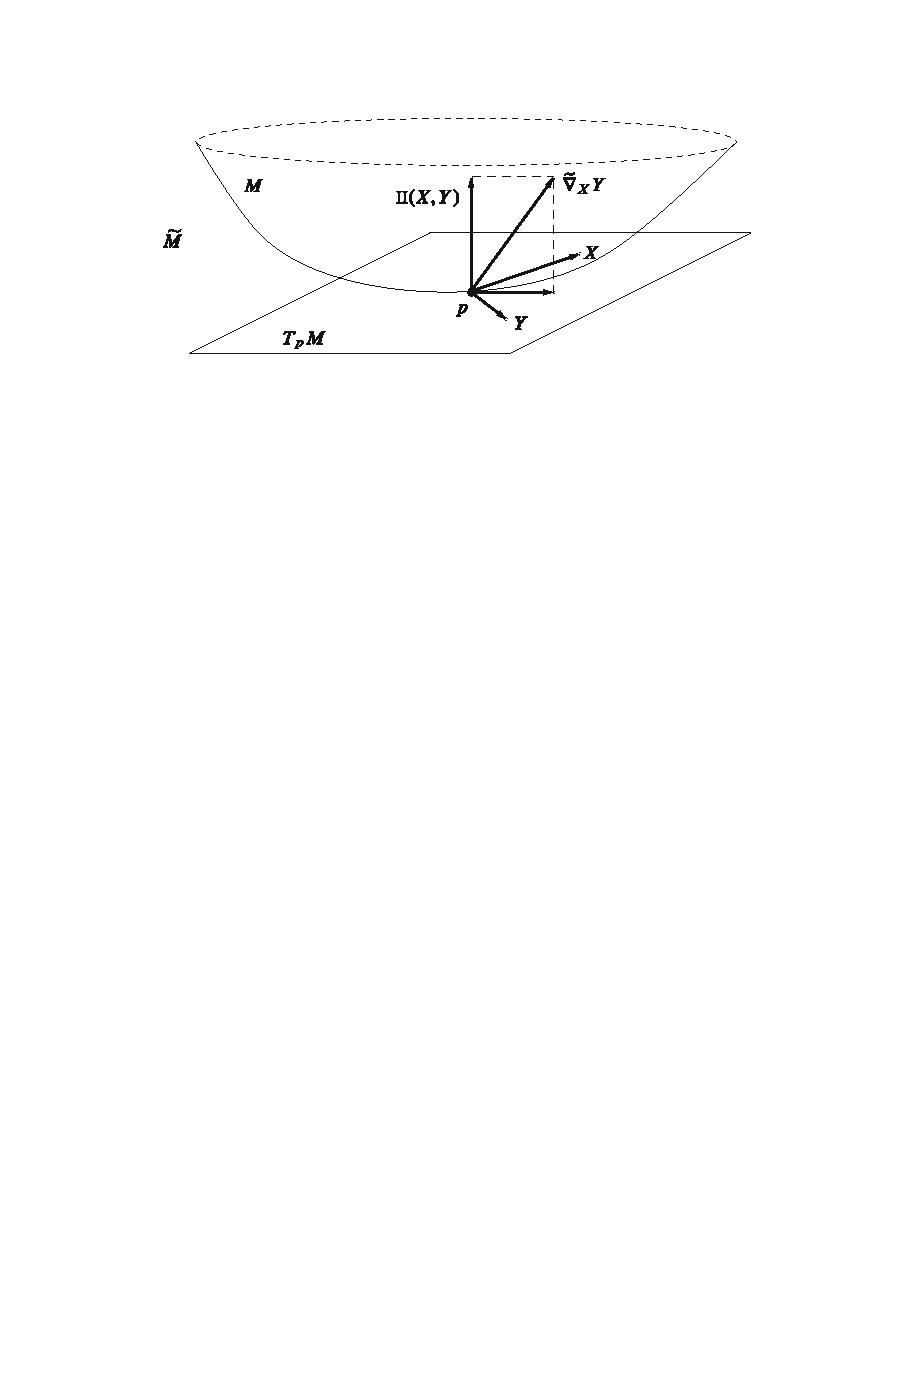
\includegraphics{pictures/second-fundamental-form}
\caption{The second fundamental form.}
\end{figure}
\begin{proposition}[\textbf{Properties of the Second Fundamental Form}]\label{Riemann second form prop}
Suppose $(M,g)$ is an embedded Riemannian submanifold of a (pseudo-)Riemannian manifold $(\widetilde{M},\tilde{g})$, and let $X,Y\in\X(M)$.
\begin{itemize}
\item[(a)] $\Two(X,Y)$ is independent of the extensions of $X$ and $Y$ to an open subset of $\widetilde{M}$.
\item[(b)] $\Two(X,Y)$ is bilinear over $C^\infty(M)$ in $X$ and $Y$.
\item[(c)] $\Two(X,Y)$ is symmetric in $X$ and $Y$.
\item[(d)] The value of $\Two(X,Y)$ at a point $p\in M$ depends only on $X_p$ and $Y_p$.
\end{itemize}
\end{proposition}
\begin{proof}
Choose particular extensions of $X$ and $Y$ to a neighborhood of $M$ in $\widetilde{M}$, and for simplicity denote the extended vector fields also by $X$ and $Y$. We begin by proving that $\Two(X,Y)$ is symmetric in $X$ and $Y$ when defined in terms of these extensions. The symmetry of the connection $\widetilde{\nabla}$ implies
\[\Two(X,Y)-\Two(Y,X)=(\widetilde{\nabla}_XY)^\bot-(\widetilde{\nabla}_YX)^\bot=[X,Y]^\bot.\]
Since $X$ and $Y$ are tangent to $M$ at all points of $M$, so is their Lie bracket (Corollary~\ref{Lie bracket tangent to submani}). Therefore $[X,Y]^\bot=0$, so $\Two$ is symmetric.\par
Because $\widetilde{\nabla}_XY$ depends only on $X_p$, it follows that the value of $\Two(X,Y)$ at $p$ depends only on $X_p$, and in particular is independent of the extension chosen for $X$. Because $\widetilde{\nabla}_XY$ is linear over $C^\infty(\widetilde{M})$ in $X$, and every $f\in C^\infty(M)$ can be extended to a smooth function on a neighborhood of $M$ in $\widetilde{M}$, it follows that $\Two(X,Y)$ is linear over $C^\infty(M)$ in $X$. By symmetry, the same claims hold for $Y$.
\end{proof}
As a consequence of the preceding proposition, for every $p\in M$ and all vectors $v,w\in T_pM$, it makes sense to interpret $\Two(v,w)$ as the value of $\Two(V,W)$ at $p$, where $V$ and $W$ are any vector fields on $M$ such that $V_p=v$ and $W_p=w$, and we will do so from now on without further comment.\par
We have not yet identified the tangential term in the decomposition of $\widetilde{\nabla}_XY$. Proposition~\ref{Levi-Civita Euclidean}(b) showed that in the special case of a submanifold of a Euclidean or pseudo-Euclidean space, it is none other than the covariant derivative with respect to the Levi-Civita connection of the induced metric on $M$. The following theorem shows that the same is true in the general case. Therefore, we can interpret the second fundamental form as a measure of the difference between the intrinsic Levi-Civita connection on $M$ and the ambient Levi-Civita connection on $\widetilde{M}$.
\begin{theorem}[\textbf{Guass formula}]\label{Riemann Levi-Civita submani}
Suppose $(M,g)$ is an embedded Riemannian submanifold of a (pseudo-)Riemannian manifold $(\widetilde{M},\tilde{g})$. If $X,Y\in\X(M)$ are extended arbitrarily to smooth vector fields on a neighborhood of $M$ in $\widetilde{M}$, the following formula holds along $M$:
\[\widetilde{\nabla}_XY=\nabla_XY+\Two(X,Y).\]
\end{theorem}
\begin{proof}
Because of the decomposition $(\ref{Riemann connection submani decomp})$ and the definition of the second fundamental form, it suffices to show that $(\widetilde{\nabla}_XY)^\top=\nabla_XY$ at all points of $M$.\par
Define a map $\nabla^{\top}:\X(M)\to\X(M)\to\X(M)$ by
\[\nabla^{\top}_XY=(\widetilde{\nabla}_XY)^\top.\]
where $X$ and $Y$ are extended arbitrarily to an open subset of $\widetilde{M}$. We examined a special case of this construction, in which $\tilde{g}$ is a Euclidean or pseudo-Euclidean metric, in Example~\ref{Euclidean tangential connection}. It follows exactly as in that example that $\nabla^{\top}$ is a connection on $M$, and exactly as in the proofs of Propositions~\ref{Euclidean tangential connection metric} and \ref{Euclidean tangential connection symmetric} that it is symmetric and compatible with $g$. The uniqueness of the Riemannian connection on $M$ then shows that $\nabla^{\top}=\nabla$.
\end{proof}
The Gauss formula can also be used to compare intrinsic and extrinsic covariant derivatives along curves. If $\gamma:I\to M$ is a smooth curve and $X$ is a vector field along $\gamma$ that is everywhere tangent to $M$, then we can regard $X$ as either a vector field along $\gamma$ in $\widetilde{M}$ or a vector field along $\gamma$ in $M$. We let $\widetilde{D}_tX$ and $D_tX$ denote its covariant derivatives along $\gamma$ as a curve in $\widetilde{M}$ and as a curve in $M$, respectively.\par
The next corollary shows how the two covariant derivatives are related.
\begin{corollary}[\textbf{The Gauss Formula Along a Curve}]
Suppose $(M,g)$ is an embedded Riemannian submanifold of a (pseudo-)Riemannian manifold $(\widehat{M},\tilde{g})$, and $\gamma:I\to M$ is a smooth curve. If $X$ is a smooth vector field along $\gamma$ that is everywhere tangent to $M$, then
\begin{align}\label{Riemann connection submani curve-1}
\widetilde{D}_tX=D_tX+\Two(\gamma',X).
\end{align}
\end{corollary}
\begin{proof}
For each $t_0\in I$, we can find an adapted orthonormal frame $(E_1,\dots,E_m)$ in a neighborhood of $\gamma(t_0)$. (Recall that our default assumption is that $\dim M=m$ and $\dim M=n$.) In terms of this frame, $X$ can be written $X(t)=\sum_{i=1}^{n}X^iE_i|_{\gamma(t)}$. Applying the product rule and the Gauss formula, and using the fact that each 
vector field $E_i$ is extendible, we get
\begin{align*}
\widetilde{D}_tX&=\sum_{i=1}^{n}(\dot{X}^iE_i+X^i\widetilde{\nabla}_{\gamma'}E_i)\\
&=\sum_{i=1}^{n}(\dot{X}^iE_i+X^i\nabla_{\gamma'}E_i+X^i\Two(\gamma',E_i))\\
&=D_tX+\Two(\gamma',X).
\end{align*}
This gives the claim.
\end{proof}
Although the second fundamental form is defined in terms of covariant derivatives of vector fields tangent to $M$, it can also be used to evaluate extrinsic covariant derivatives of normal vector fields, as the following proposition shows. To express it concisely, we introduce one more notation. For each normal vector field $N\in NM$, we obtain a scalar-valued symmetric bilinear form $\Two_N:\X(M)\times\X(M)\to C^{\infty}(M)$ by
\[\Two_N(X,Y)=\langle\Two(X,Y),N\rangle.\]
Let $W_N:\X(M)\to\X(M)$ denote the self-adjoint linear map associated with this bilinear form, characterized by
\begin{align}\label{Riemann Weingarten def}
\langle W_N(X),Y\rangle=\Two_N(X,Y)=\langle\Two(X,Y),N\rangle.
\end{align}
The map $W_N$ is called the \textbf{Weingarten map in the direction of $\bm{N}$}. Because the second fundamental form is bilinear over $C^\infty(M)$, it follows that $W_N$ is linear over $C^\infty(M)$ and thus defines a smooth bundle homomorphism from $TM$ to itself.
\begin{proposition}[\textbf{The Weingarten Equation}]
Suppose $(M,g)$ is an embedded Riemannian submanifold of a (pseudo-)Riemannian manifold $(\widetilde{M},\tilde{g})$. For every $X\in\X(M)$ and $N\in NM$, the following equation holds:
\begin{align}\label{Riemann Weingarten Equation}
W_N(X)=-(\widetilde{\nabla}_XN)^{\top}.
\end{align}
when $N$ is extended arbitrarily to an open subset of $\widetilde{M}$.
\end{proposition}
\begin{proof}
Note that at points of $M$, the covariant derivative $\widetilde{\nabla}_XN$ is independent of the choice of extensions of $X$ and $N$ by Proposition~\ref{connection local curve}. Let $Y\in\X(M)$ be arbitrary, extended to a vector field on an open subset of $\widetilde{M}$. Since $\langle Y,N\rangle$ vanishes identically along $M$ and $X$ is tangent to $M$, the following holds at points of $M$:
\begin{align*}
0&=X\langle N,Y\rangle\\
&=\langle\widetilde{\nabla}_XN,Y\rangle+\langle N,\widetilde{\nabla}_XY\rangle\\
&=\langle\widetilde{\nabla}_XN,Y\rangle+\langle N,\nabla_XY+\Two(X,Y)\rangle\\
&=\langle\widetilde{\nabla}_XN,Y\rangle+\langle N,\Two_N(X,Y)\rangle\\
&=\langle\widetilde{\nabla}_XN,Y\rangle+\langle W_N(X),Y\rangle.
\end{align*}
Since $Y$ was an arbitrary vector field tangent to $M$, this implies
\[0=(\widetilde{\nabla}_XN+W_N(X))^{\top}=(\widetilde{\nabla}_XN)^\top+W_N(X).\]
which is equivalent to $(\ref{Riemann Weingarten Equation})$.
\end{proof}
In addition to describing the difference between the intrinsic and extrinsic connections, the second fundamental form plays an even more important role in describing the difference between the curvature tensors of $\widetilde{M}$ and $M$. The explicit formula, also due to Gauss, is given in the following theorem.
\begin{theorem}[\textbf{The Gauss Equation}]
Suppose $(M,g)$ is an embedded Riemannian submanifold of a (pseudo-)Riemannian manifold $(\widetilde{M},\tilde{g})$. For all $X,Y,V,W\in\X(M)$, the following equation holds:
\begin{align}\label{Riemann submani Guass equation}
R(X,Y,V,W)=\langle\Two(X,W),\Two(Y,V)\rangle-\langle\Two(X,V),\Two(Y,W)\rangle+\tilde{R}(X,Y,V,W).
\end{align}
\end{theorem}
\begin{proof}
Let $X,Y,V,W$ be extended arbitrarily to an open subset of $\widetilde{M}$. At points of $M$, using the definition of the curvature and the Gauss formula, we get
\begin{align*}
\langle\widetilde{\nabla}_X\widetilde{\nabla}_YV,W\rangle&=\langle\widetilde{\nabla}_X(\nabla_YV+\Two(Y,V)),W\rangle\\
&=\langle\widetilde{\nabla}_X\nabla_YV,W\rangle+\langle\widetilde{\nabla}_X\Two(Y,V),W\rangle\\
&=\langle\nabla_X\nabla_YV,W\rangle+\langle\Two(X,\nabla_YV),W\rangle+\widetilde{\nabla}_X\langle\Two(Y,V),W\rangle-\langle\Two(Y,V),\widetilde{\nabla}_XW\rangle\\
&=\langle\nabla_X\nabla_YV,W\rangle-\langle\Two(Y,V),\widetilde{\nabla}_XW\rangle\\
&=\langle\nabla_X\nabla_YV,W\rangle-\langle\Two(Y,V),\nabla_XW\rangle-\langle\Two(Y,V),\Two(X,W)\rangle\\
&=\langle\nabla_X\nabla_YV,W\rangle-\langle\Two(Y,V),\Two(X,W)\rangle,
\end{align*}
and
\begin{align*}
\langle\widetilde{\nabla}_{[X,Y]}V,W\rangle&=\langle\nabla_{[X,Y]}V,W\rangle+\langle\Two([X,Y],V),W\rangle=\langle\nabla_{[X,Y]}V,W\rangle.
\end{align*}
These together give
\begin{align*}
\tilde{R}(X,Y,V,W)&=\langle\nabla_X\nabla_YV-\nabla_Y\nabla_XV-\nabla_{[X,Y]}V,W\rangle-\langle\Two(Y,V),\Two(X,W)\rangle\\
&\,+\langle\Two(X,V),\Two(Y,W)\rangle\\
&=R(X,Y,V,W)-\langle\Two(Y,V),\Two(X,W)\rangle+\langle\Two(X,V),\Two(Y,W)\rangle
\end{align*}
which is equivalent to $(\ref{Riemann submani Guass equation})$.
\end{proof}
There is one other fundamental submanifold equation, which relates the normal part of the ambient curvature endomorphism to derivatives of the second fundamental form. 
We will not have need for it, but we include it here for completeness. To state it, we need to introduce a connection on the normal bundle of a Riemannian submanifold.\par
If $(M,g)$ is a Riemannian submanifold of a (pseudo-)Riemannian manifold $(\widetilde{M},\tilde{g})$, the \textbf{normal connection} 
$\nabla^{\bot}:\X(M)\times\Gamma(NM)\to\Gamma(NM)$ 
is defined by
\[\nabla^{\bot}_XN=(\widetilde{\nabla}_XN)^{\bot}.\]
where $N$ is extended to a smooth vector field on a neighborhood of $M$ in $\widetilde{M}$.
\begin{proposition}
If $(M,g)$ is an embedded Riemannian submanifold of a (pseudo-)Riemannian manifold $(\widetilde{M},\tilde{g})$, then $\nabla^{\bot}$ is a well-defined 
connection in $NM$, which is compatible with $\tilde{g}$ in the sense that for any two sections $N_1,N_2$ of $NM$ and every $X\in\X(M)$, we have
\[X\langle N_1,N_2\rangle=\langle\nabla^{\bot}_XN_1,N_2\rangle+\langle N_1,\nabla^{\bot}_XN_2\rangle.\]
\end{proposition}
\begin{proof}
The map $\pi^{\bot}:T\widetilde{M}|_M\to NM$ is a smooth bundle homomorphism, so it is clear that $\nabla^{\bot}$ satisfies the conditions of connections since $\nabla$ does. 
The metric compactibility also follows from this.
\end{proof}
We need the normal connection primarily to make sense of tangential covariant derivatives of the second fundamental form. To do so, we make the following definitions. 
Let $E\to M$ denote the bundle whose fiber at each point $p\in M$ is the set of bilinear maps $T_pM\times T_pM\to N_pM$. It is easy to check that $E$ is a smooth vector 
bundle over $M$, and that smooth sections of $E$ correspond to smooth maps $\X(M)\times\X(M)\to\Gamma(NM)$ that are bilinear over $C^\infty(M)$, such as the second 
fundamental form. Define a connection $\nabla^E$ in $E$ as follows: if $B$ is any smooth section of $E$, let $\nabla^E_XB$ be the smooth section of $E$ defined by
\[(\nabla^E_XB)(Y,Z)=\nabla_X^{\bot}(B(Y,Z))-B(\nabla_XY,Z)-B(Y,\nabla_XZ).\]
Now we are ready to state the last of the fundamental equations for submanifolds.
\begin{theorem}[\textbf{The Codazzi Equation}]
Suppose $(M,g)$ is an embedded Riemannian submanifold of a (pseudo-)Riemannian manifold $(\widetilde{M},\tilde{g})$. For all $X,Y,Z\in\X(M)$ the following 
equation holds:
\begin{align}\label{Riemann Codazzi equation-1}
(\tilde{R}(X,Y)Z)^{\bot}=(\nabla^E_X\Two)(Y,Z)-(\nabla^E_Y\Two)(X,Z).
\end{align}
\end{theorem}
\begin{proof}
It suffices to show that both sides of $(\ref{Riemann Codazzi equation-1})$ give the same result when we take their inner products with an arbitrary smooth normal vector 
field $N$ along $M$:
\begin{align}\label{Riemann Codazzi equation-2}
\langle\tilde{R}(X,Y)Z,N\rangle=\langle(\nabla^E_X)(Y,Z),N\rangle-\langle(\nabla^E_Y)(X,Z),N\rangle
\end{align}
We begin as in the proof of the Gauss equation: after extending the vector fields to a neighborhood of $M$ and applying the Gauss formula, we obtain
\begin{align*}
\tilde{R}(X,Y,Z,N)&=\langle\widetilde{\nabla}_X(\nabla_YZ+\Two(Y,Z))-\widetilde{\nabla}_Y(\nabla_XZ+\Two(X,Z))-\widetilde{\nabla}_{[X,Y]}Z,N\rangle
\end{align*}
Now when we expand the covariant derivatives, we need only pay attention to the normal components. This yields
\begin{align*}
\tilde{R}(X,Y,Z,N)&=\langle\Two(X,\nabla_YZ)+(\nabla^E_X\Two)(Y,Z)+\Two(\nabla_XY,Z)+\Two(Y,\nabla_XZ),N\rangle\\
&-\langle\Two(Y,\nabla_XZ)+(\nabla^E_Y\Two)(X,Z)+\Two(\nabla_YX,Z)+\Two(X,\nabla_YZ),N\rangle\\
&-\langle\Two([X,Y],Z),N\rangle\\
&=\langle(\nabla^E_X)(Y,Z),N\rangle-\langle(\nabla^E_Y)(X,Z),N\rangle+\langle\nabla_XY-\nabla_YX-[X,Y],N\rangle\\
&=\langle(\nabla^E_X)(Y,Z),N\rangle-\langle(\nabla^E_Y)(X,Z),N\rangle.
\end{align*}
This finishes the proof.
\end{proof}
\subsubsection{Curvature of a curve}
By studying the curvatures of curves, we can give a more geometric interpretation of the second fundamental form. Suppose $(M,g)$ is a (pseudo-)Riemannian manifold, and $\gamma:I\to M$ is a smooth unit-speed curve in $M$. We define the \textbf{geodesic curvature} of $\gamma$ as the length of the acceleration vector field, which is  the function $\kappa:I\to\R$ given by
\[\kappa(t)=|D_t\gamma'(t)|.\]
If $\gamma$ is an arbitrary regular curve in a Riemannian manifold (not necessarily of unit speed), we first find a unit-speed reparametrization $\tilde{\gamma}=\gamma\circ\varphi$, and then define the curvature of $\gamma$ at $t$ to be the curvature of $\tilde{\gamma}$ at $\varphi^{-1}(t)$. In a pseudo-Riemannian manifold, the same approach works, but we have to restrict the definition to curves $\gamma$ such that $|\gamma'(t)|$ is everywhere nonzero.\par
From the definition, it follows that a smooth unit-speed curve has vanishing geodesic curvature if and only if it is a geodesic, so the geodesic curvature of a curve can be regarded as a quantitative measure of how far it deviates from being a geodesic. If $M=\R^n$ with the Euclidean metric, the geodesic curvature agrees with the notion of curvature introduced in advanced calculus courses.\par
Now suppose $(\widetilde{M},\tilde{g})$ is a (pseudo-)Riemannian manifold and $(M,g)$ is a Riemannian submanifold. Every regular curve $\gamma:I\to M$ has two distinct geodesic curvatures: its \textbf{intrinsic curvature} $\kappa$ as a curve in $M$, and its \textbf{extrinsic curvature} $\widetilde{\kappa}$ as a curve 
in $\widetilde{M}$. The second fundamental form can be used to compute the relationship between the two.
\begin{proposition}
Suppose $(M,g)$ is an embedded Riemannian submanifold of a (pseudo-)Riemannian manifold $(\widetilde{M},\tilde{g})$, $p\in M$, and $v\in T_pM$.
\begin{itemize}
\item[(a)] $\Two(v,v)$ is the $\tilde{g}$-acceleration at $p$ of the $g$-geodesic $\gamma_v$.
\item[(b)] If $v$ is a unit vector, then $|\Two(v,v)|$ is the $\tilde{g}$-curvature of $\gamma_v$ at $p$.
\end{itemize}
\end{proposition}
\begin{proof}
Suppose $\gamma:(-\eps,\eps)\to M$ is any regular curve with $\gamma(0)=p$ and $\gamma'(0)=v$. Applying the Gauss formula (Corollary~\ref{Riemann connection submani curve-1}) 
to the vector field $\gamma'$ along $\gamma$, we obtain
\[\widetilde{D}_t\gamma'=D_t\gamma+\Two(\gamma',\gamma').\]
If $\gamma$ is a $g$-geodesic in $M$, this formula simplifies to
\[\widetilde{D}_t\gamma'=\Two(\gamma',\gamma').\]
Both conclusions of the proposition follow from this.
\end{proof}
Note that the second fundamental form is completely determined by its values of the form $\Two(v,v)$ for unit vectors $v$, by the following lemma.
\begin{lemma}\label{Bilinear symmetric form lemma}
Suppose $V$ is an inner product space, $W$ is a vector space, and $B,B':V\times V\to W$ are symmetric and bilinear. If $B(v,v)=B'(v,v)$ for every unit vector $v\in V$, 
then $B=B'$.
\end{lemma}
\begin{proof}
Every vector $v\in V$ can be written $v=|v|\hat{v}$ for some unit vector $\hat{v}$, so the bilinearity of $B$ and $B'$ implies $B(v,v)=B'(v,v)$ for every $v$, 
not just unit vectors. The result then follows from the following polarization identity for inner products:
\begin{equation*}
B(v,w)=\frac{1}{4}(B(v+w,v+w)-B(v-w,v-w)).\tag*{\qedhere}
\end{equation*}
\end{proof}
Because the intrinsic and extrinsic accelerations of a curve are usually different, it is generally not the case that a $\tilde{g}$-geodesic that starts tangent to 
$M$ stays in $M$; just think of a sphere in Euclidean space, for example. A Riemannian submanifold $(M,g)$ of $(\widetilde{M},\tilde{g})$ is said to be \textbf{totally 
geodesic} if every $\tilde{g}$-geodesic that is tangent to $M$ at some time $t_0$ stays in $M$ for all $t$ in some interval $(t_0-\eps,t_0+\eps)$.
\begin{proposition}
Suppose $(M,g)$ is an embedded Riemannian submanifold of a (pseudo-)Riemannian manifold $(\widetilde{M},\tilde{g})$, The following are equivalent:
\begin{itemize}
\item[(a)] $M$ is totally geodesic in $\widetilde{M}$. 
\item[(b)] Every $g$-geodesic in $M$ is also a $\tilde{g}$-geodesic in $\widetilde{M}$.
\item[(c)] The second fundamental form of $M$ vanishes identically.
\item[(d)] If $\gamma:I\to M$ is a curve in $M$, $t_0\in I$ and $v\in T_{\gamma(t_0)}M$. Then the parallel transport of $v$ along $\gamma$ is the same for $M$ and 
for $\widetilde{M}$. 
\end{itemize}
\end{proposition}
\begin{proof}
We will prove $(a)\Rightarrow(b)\Rightarrow(c)\Rightarrow(a)$. First assume that $M$ is totally geodesic. Let $\gamma:I\to M$ be a $g$-geodesic. For each $t_0\in I$, let $\tilde{\gamma}:\widetilde{I}\to\widetilde{M}$ 
be the $\tilde{g}$-geodesic with $\tilde{\gamma}(t_0)=\gamma(t_0)$ and $\tilde{\gamma}'(t_0)=\gamma'(t_0)$. The hypothesis implies that there is some open 
interval $I_0$ containing $t_0$ such that $\tilde{\gamma}(t)\in M$ for $t\in I_0$. On $I_0$, the Gauss formula $(\ref{Riemann connection submani curve-1})$ 
for $\tilde{\gamma}'$ reads
\[0=\widetilde{D}_t\tilde{\gamma}'=D_t\tilde{\gamma}'+\Two(\tilde{\gamma}',\tilde{\gamma}').\]
Because the first term on the right is tangent to $M$ and the second is normal, the two terms must vanish individually. In particular, $D_t\tilde{\gamma}'\equiv 0$ on 
$I_0$, which means that $\tilde{\gamma}$ is also a $g$-geodesic there. By uniqueness of geodesics, therefore, $\gamma=\tilde{\gamma}$ on $I_0$, so it follows in 
turn that $\gamma$ is a $\tilde{g}$-geodesic there. Since the same is true in a neighborhood of every $t_0\in I$, it follows that $\gamma$ is a $\tilde{g}$-geodesic 
on its whole domain.\par
Next assume that every $g$-geodesic is a $\tilde{g}$-geodesic. Let $p\in M$ and $v\in T_pM$ be arbitrary, and let $\gamma:I\to M$ be the $g$-geodesic with $\gamma(0)=p$ 
and $\gamma'(0)=v$. The hypothesis implies that $\gamma$ is also a $\tilde{g}$-geodesic. Thus $\widetilde{D}_t\gamma'=D_t\gamma'=0$, so the Gauss formula yields 
$\Two(\gamma',\gamma')=0$ along $\gamma$. In particular, $\Two(v,v)=0$. By Lemma~\ref{Bilinear symmetric form lemma}, this implies that $\Two$ is identically zero.\par
Now assume that $\Two=0$, and let $\tilde{\gamma}:\widetilde{I}\to\widetilde{M}$ be a $\tilde{g}$-geodesic such that $\tilde{\gamma}(t_0)\in M$ and 
$\tilde{\gamma}'(t_0)\in TM$ for some $t_0\in I$. Let $\gamma:I\to M$ be the $g$-geodesic with the same initial conditions: $\gamma(t_0)=\tilde{\gamma}(t_0)$ 
and $\gamma'(t_0)=\tilde{\gamma}'(t_0)$. The Gauss formula together with the hypothesis $\Two=0$ implies that $\widetilde{D}_t\gamma'=D_t\gamma'=0$, so $\gamma$ is 
also a $\tilde{g}$-geodesic. By uniqueness of geodesics, therefore, $\tilde{\gamma}=\gamma$ on the intersection of their domains, which implies that $\tilde{\gamma}$ 
lies in $M$ for $t$ in some open interval around $t_0$.\par
Finally, recall that the parallel transport is defined by the unique vector field $V$ along $\gamma$ such that $D_tV\equiv 0$ and $V(t_0)=v$. In view of the Guass formula $(\ref{Riemann connection submani curve-1})$, 
it is clear that $(c)\Rightarrow(d)$ and $(d)\Rightarrow(b)$. Therefore we are done.
\end{proof}
\subsection{Hypersurfaces}
Now we specialize the preceding considerations to the case in which $M$ is a hypersurface (i.e., a submanifold of codimension $1$) in $\widetilde{M}$. Throughout this part, 
our default assumption is that $(M,g)$ is an embedded $n$-dimensional Riemannian submanifold of an $n+1$-dimensional Riemannian manifold $(\widetilde{M},\tilde{g})$.
In this situation, at each point of $M$ there are exactly two unit normal vectors. In terms of any local adapted orthonormal frame $(E_1,\dots,E_{n+1})$, the two choices 
are $E_{n+1}$. In a small enough neighborhood of each point of $M$, therefore, we can always choose a smooth unit normal vector field along $M$.\par
If both $M$ and $\widetilde{M}$ are orientable, we can use an orientation to pick out a global smooth unit normal vector field along all of $M$. In general, though, 
this might or might not be possible. Since all of our computations in this chapter are local, we will always assume that we are working in a small enough neighborhood 
that a smooth unit normal field exists. We will address as we go along the question of how various quantities depend on the choice of normal vector field.
\subsubsection{The scalar second fundamental form and the shape operator}
Having chosen a distinguished smooth unit normal vector field $N$ on the hypersurface $M\sub\widetilde{M}$, we can replace the vector-valued second fundamental form 
$\Two$ by a simpler scalar-valued form. The \textbf{scalar second fundamental form} of $M$ is the symmetric covariant $2$-tensor field $h\in\Gamma(\Sigma^2T^*M)$ defined 
by $h=\Two_N$; in other words,
\[h(X,Y)=\langle\Two(X,Y),N\rangle.\]
Using the Gauss formula $\widetilde{\nabla}_XY=\nabla_XY+\Two(X,Y)$ and noting that $\nabla_XY$ is orthogonal to $N$, we can rewrite the definition as
\[h(X,Y)=\langle\widetilde{\nabla}_XY,N\rangle.\]
Also, since $N$ is a unit vector spanning $NM$ at each point, the definition of $h$ is equivalent to
\begin{align}\label{Riemann shapre operator hypersurface}
\Two(X,Y)=h(X,Y)N.
\end{align}
Note that replacing $N$ by $-N$ multiplies $h$ by $-1$, so the sign of $h$ depends on which unit normal is chosen; but $h$ is otherwise independent of the choices.\par
The choice of unit normal field also determines a Weingarten map $W_N:\X(M)\to\X(M)$ by $(\ref{Riemann Weingarten def})$; in the case of a hypersurface, we use the notation $s=W_N$ and call it the \textbf{shape operator} of $M$. Alternatively, we can think of $s$ as the $(1,1)$-tensor field on $M$ obtained from $h$ by raising an index. It is characterized by
\[\langle s(X),Y\rangle=h(X,Y)\for X,Y\in\X(M).\]
Because $h$ is symmetric, $s$ is a self-adjoint endomorphism of $TM$, that is,
\[\langle s(X),Y\rangle=\langle X,s(Y)\rangle\for X,Y\in\X(M).\]
As with $h$, the sign of $s$ depends on the choice of $N$.\par
\begin{theorem}[\textbf{Fundamental Equations for a Hypersurface}]
Suppose $(M,g)$ is a Riemannian hypersurface in a Riemannian manifold $(\widetilde{M},\tilde{g})$, and $N$ is a smooth unit normal vector field along $M$.
\begin{itemize}
\item[(a)] The Guass formula for a hypersurface: If $X,Y\in\X(M)$ are extended to an open subset of $\widetilde{M}$, then
\[\widetilde{\nabla}_XY=\nabla_XY+h(X,Y)N.\] 
\item[(b)] The Guass formula for a curve in a hypersurface: If $\gamma:I\to M$ is a smooth curve and $X:I\to TM$ is a smooth vector field along $\gamma$, then
\[\widetilde{D}_tX=D_tX+h(\gamma',X)N.\] 
\item[(c)] The Weingarten equation for a hypersurface: For every $X\in\X(M)$,
\begin{align}\label{Riemann Weigarten equation hypersurface}
sX=-\widetilde{\nabla}_XN.
\end{align}
\item[(d)] The Guass equation for a hypersurface: For all $X,Y,V,W\in\X(M)$,
\begin{align}\label{Riemann Guass equation hypersurface}
R(X,Y,V,W)=\tilde{R}(X,Y,V,W)+\frac{1}{2}(h\owedge h)(X,Y,V,W).
\end{align}
\item[(e)] The Codazzi equation for a hypersurface: For all $X,Y,V,W\in\X(M)$,
\begin{align}\label{Riemann Codazzi equation hypersurface}
\tilde{R}(X,Y,Z,N)=(Dh)(Z,X,Y).
\end{align}
\end{itemize}
\end{theorem}
\begin{proof}
Parts (a), (b), and (d) follow immediately from substituting $(\ref{Riemann shapre operator hypersurface})$ into the general versions of the Gauss formula and 
Gauss equation. To prove (c), note first that the general version of theWeingarten equation can be written $(\widetilde{\nabla}_XN)^{\top}=-sX$. Since 
$\langle\widetilde{\nabla}_XN,N\rangle=X(|N|^2)/2=0$, it follows  that $\nabla_XN$ is tangent to $M$, so (c) follows.\par
To prove the hypersurface Codazzi equation, note that the fact that $N$ is a unit vector field implies
\[0=X|N|^2=2\langle\nabla^{\bot}_XN,N\rangle.\]
Since $N$ spans the normal bundle, this implies that $N$ is parallel with respect to the normal connection. Moreover
\begin{align*}
(\nabla^E_X\Two)(Y,Z)&=\nabla^{\bot}_XY(\Two(Y,Z))-\Two(\nabla_XY,Z)-\Two(Y,\nabla_XZ)\\
&=\nabla^{\bot}_XY(h(Y,Z)N)-\Two(\nabla_XY,Z)-\Two(Y,\nabla_XZ)\\
&=\big(X(h(X,Y))-h(\nabla_XY,Z)-h(Y,\nabla_XZ)\big)N\\
&=(\nabla_Xh)(Y,Z)N.
\end{align*}
Inserting this into the general form $(\ref{Riemann Codazzi equation-1})$ of the Codazzi equation and using the fact that $\nabla h$ is symmetric in its first two indices 
yields
\begin{align*}
\tilde{R}(X,Y,Z,N)&=(\nabla_Xh)(Y,Z)-(\nabla_Yh)(X,Z)\\
&=(\nabla h)(Y,Z,X)-(\nabla h)(X,Z,Y)\\
&=-(\nabla h)(Z,X,Y)+(\nabla h)(Z,Y,X).
\end{align*}
which is equivalent to $(\ref{Riemann Codazzi equation hypersurface})$.
\end{proof}
\subsubsection{Principal curvatures}
At every point $p\in M$, we have seen that the shape operator $s$ is a self-adjoint linear endomorphism of the tangent space $T_pM$. To analyze such an operator, we 
recall some linear-algebraic facts about self-adjoint endomorphisms.
\begin{lemma}
Suppose $V$ is a finite-dimensional inner product space and $s:V\to V$ is a self-adjoint linear endomorphism. Let $S$ denote the set of unit vectors in $V$. There is a 
vector $v_0\in S$ where the function $v\mapsto\langle sv,v\rangle$ achieves its maximum among elements of $S$, and every such vector is an eigenvector of $s$ with 
eigenvalue $\lambda_0=\langle sv_0,v_0\rangle$.
\end{lemma}
\begin{proposition}
Suppose $V$ is a finite-dimensional inner product space and $s:V\to V$ is a self-adjoint linear endomorphism. Then $V$ has an orthonormal basis of $s$-eigenvectors, and 
all of the eigenvalues are real.
\end{proposition}
Applying this proposition to the shape operator $s:T_pM\to T_pM$, we see that $s$ has real eigenvalues $\kappa_1,\dots,\kappa_n$, and there is an orthonormal basis 
$(e_1,\dots,e_n)$ for $T_pM$ consisting of $s$-eigenvectors, with $se_i=\lambda_ie_i$ for each $i$ (no summation). In this basis, both $h$ and $s$ are represented by 
diagonal matrices, and $h$ has the expression
\[h(v,w)=\kappa_1v^1w^1+\cdots+\kappa_nv^nw^n.\]
The eigenvalues of $s$ at a point $p\in M$ are called the principal curvatures of $M$ at $p$, and the corresponding eigenspaces are called the \textbf{principal directions}. 
The principal curvatures all change sign if we reverse the normal vector, but the principal directions and principal curvatures are otherwise independent of the choice 
of coordinates or bases.\par
There are two combinations of the principal curvatures that play particularly important roles for hypersurfaces. The \textbf{Gaussian curvature} is defined as $K=\det(s)$, and 
the \textbf{mean curvature} as $H=\tr(s)/n=\tr_g(h)/n$. Since the determinant and trace of a linear endomorphism are basis-independent, these are well defined once a 
unit normal is chosen. In terms of the principal curvatures, they are
\[K=\kappa_1\cdots\kappa_n,\quad H=\frac{1}{n}(\kappa_1+\cdots+\kappa_n).\]
as can be seen by expressing $s$ in terms of an orthonormal basis of eigenvectors. If $N$ is replaced by $-N$, then $H$ changes sign, while $K$ is multiplied by $(-1)^n$.
\subsubsection{Computations in semigeodesic coordinates}
Semigeodesic coordinates (Proposition~\ref{Riemann semigeodesic char}) provide an extremely convenient tool for computing the invariants of hypersurfaces.\par
Let $(\widetilde{M},\tilde{g})$ be an $(n+1)$-dimensional Riemannian manifold, and let $(x^1,\dots,x^n,v)$ be semigeodesic coordinates on an open subset $U\sub\widetilde{M}$. 
(For example, they might be Fermi coordinates for the hypersurface $M=v^{-1}(0)$.) For each real number $a$ such that $v^{-1}(a)\neq\emp$, the level set $M_a=v^{-1}(a)$ 
is a properly embedded hypersurface in $U$. Let $g_a$ denote the induced metric on $M_a$. Corollary~\ref{Riemann semigeodesic Christoffel} shows that $\tilde{g}$ is 
given by
\begin{align}\label{Riemann hypersurface semigeodesic metric}
\tilde{g}=dv^2+g_{\alpha\beta}dx^\alpha dx^\beta.
\end{align}
The restrictions of $(x^1,\dots,x^n)$ give smooth coordinates for each hypersurface $M_a$, and in those coordinates the induced metric $g_a$ is given by $g_{\alpha\beta}dx^\alpha dx^\beta$. 
(Here we use the summation convention with Greek indices running from $1$ to $n$.) The vector field $\partial_v=\partial_{n+1}$ restricts to a unit normal vector field 
along each hypersurface $M_a$.\par
As the next proposition shows, semigeodesic coordinates give us a simple formula for the second fundamental forms of all of the submanifolds $M_a$ at once.
\begin{proposition}\label{Riemann hypersurface semigeodesic curvature}
With notation as above, the components in $(x^1,\dots,x^n)$-coordinates of the scalar second fundamental form, the shape operator, and the mean curvature of $(M_a,g_a)$ 
(denoted by $h_a$, $s_a$ and $H_a$, respectively) with respect to the normal $N=\partial_v$ are given by
\[(h_a)_{\alpha\beta}=-\frac{1}{2}\partial_vg_{\alpha\beta}|_{v=a},\quad(s_a)^{\alpha}_{\beta}=-\frac{1}{2}g^{\alpha\gamma}\partial_vg_{\gamma\beta}|_{v=a},\quad H=-\frac{1}{2n}g^{\alpha\beta}\partial_vg_{\alpha\beta}|_{v=a}.\]
\end{proposition}
\begin{proof}
The normal component of $\widetilde{\nabla}_{\partial_\alpha}\partial_\beta$ is $\tilde{\gamma}_{\alpha\beta}^{n+1}\partial|_v$, which Corollary~\ref{Riemann semigeodesic Christoffel} 
shows is equal to $-1/2\partial_vg_{\alpha\beta}\partial_r$ (noting that the roles of $g$ and $\hat{g}$ in that corollary are being played here by $\tilde{g}$ 
and $g_a$, respectively). Equation $(\ref{Riemann semigeodesic Christoffel-1})$ evaluated at points of $M_a$ gives
\[(h_a)_{\alpha\beta}=\langle\widetilde{\nabla}_{\partial_\alpha}\partial_\beta,N\rangle=\langle-\frac{1}{2}\partial_vg_{\alpha\beta}\partial_v,\partial_v\rangle=-\frac{1}{2}\partial_vg_{\alpha\beta}.\]
The formulas for $s_a$ and $H_a$ follow by using $(g^{\alpha\gamma})$ (the inverse matrix of $(g_{\alpha\gamma})$) to raise an index and then taking the trace.
\end{proof}
\subsubsection{Minimal hypersurfaces}
A natural question that has received a great deal of attention over the past century is this: Given a simple closed curve $C$ in $\R^3$, is there an embedded or immersed 
surface $M$ with $\partial M=C$ that has least area among all surfaces with the same boundary? If so, what is it? Such surfaces are models of the soap films that are 
produced when a closed loop of wire is dipped in soapy water.\par
More generally, we can consider the analogous question for hypersurfaces in Riemannian manifolds. Suppose $M$ is a compact codimension-$1$ submanifold with nonempty 
boundary in an $n+1$-dimensional Riemannian manifold $(\widetilde{M},\tilde{g})$. By analogy with the case of surfaces in $\R^3$, it is traditional to use the term 
area to refer to the $n$-dimensional volume of $M$ with its induced Riemannian metric, and to say that $M$ is \textbf{area-minimizing} if it has the smallest area among 
all compact embedded hypersurfaces in $\widetilde{M}$ with the same boundary. One key observation is the following theorem, which is an analogue for hypersurfaces of 
Theorem~\ref{Riemann minimizing is geodesic} about length-minimizing curves.
\begin{theorem}\label{Riemann hypersurface minimizing area mean curvature}
Let $M$ be a compact codimension-$1$ submanifold with nonempty boundary in an $(n+1)$-dimensional Riemannian manifold  $(\widetilde{M},\tilde{g})$. If $M$ is 
area minimizing, then its mean curvature is identically zero.
\end{theorem}
\begin{proof}
Let $g$ denote the induced metric on $M$. The fact that $M$ minimizes area among hypersurfaces with the same boundary means, in particular, that it minimizes area among 
small perturbations of $M$ in a neighborhood of a single point. We will exploit this idea to prove that $M$ must have zero mean curvature everywhere.\par
Let $p\in\Int M$ be arbitrary, let $(x^1,\dots,x^n,v)$ be Fermi coordinates for $M$ on an open set $\widetilde{U}\sub\widetilde{M}$ containing $p$, and let 
$U=\widetilde{U}\cap M$. By taking $U$ sufficiently small, we can arrange that $U$ is a regular coordinate ball in $M$ and $\widetilde{U}\cap\partial M=\emp$. We use 
$(x^1,\dots,x^n)$ as coordinates on $M$, and observe the summation convention with Greek indices running from $1$ to $n$.
\begin{figure}[htbp]
\centering
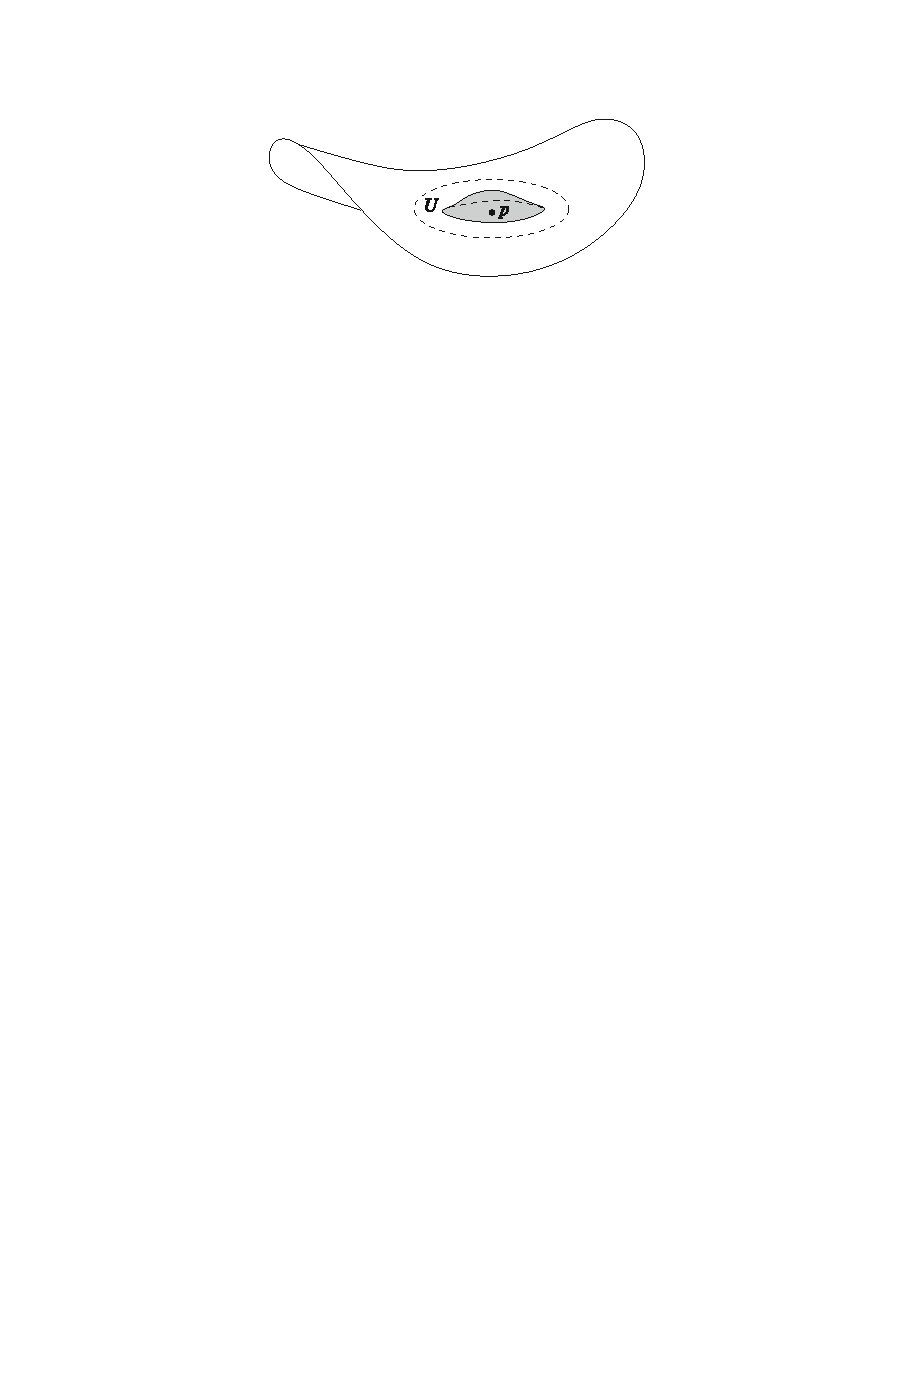
\includegraphics{pictures/minimal-surface}
\caption{The hypersurface $M_t$.}
\end{figure}

Let $\varphi$ be an arbitrary smooth real-valued function on $M$ with compact support in $U$. For sufficiently small $t$, define a set $M_t\sub\widetilde{M}$ by
\[M_t=(M\setminus U)\cup\{z\in\widetilde{U}:v(z)=t\varphi(x^1(z),\dots,x^n(z))\}.\]
Then $M_t$ is an embedded smooth hypersurface in $\widetilde{M}$, which agrees with $M$ outside of $U$ and which coincides with the graph of $v=t\varphi$ in $\widetilde{U}$. 
Let $f_t:U\to\widetilde{U}$ be the graph parametrization of $M_t\cap\widetilde{U}$, given in Fermi coordinates by
\begin{align}\label{Riemann minimal surface-1}
f_t(x^1,\dots,x^n)=(x^1,\dots,x^n,t\varphi(x)).
\end{align}
Using this map, for each $t$ we can define a diffeomorphism $F_t:M\to M_t$ by
\[F_t(z)=\begin{cases}
z,\quad z\in M\setminus\supp(\varphi),\\
f_t(z),\quad z\in U.
\end{cases}\]
For each $t$, let $\hat{g}_t=\iota_{M_t}^*\tilde{g}$ denote the induced Riemannian metric on $M_t$, and let $g_t=F_t^*\hat{g}_t=F^*\tilde{g}$ denote the 
pulled-back metric on $M$. When $t=0$, we have $M_0=M$, and both $g_0$ and $\tilde{g}_0$ are equal to the induced metric $g$ on $M$. Since $\tilde{g}$ is given 
by $(\ref{Riemann hypersurface semigeodesic metric})$ in Fermi coordinates, a simple computation shows that in $U$, $g_t=F_t^*\tilde{g}$ has the coordinate expression $g_t=(g_t)_{\alpha\beta}dx^\alpha dx^\beta$, 
where
\begin{align}\label{Riemann minimal surface-2}
(g_t)_{\alpha\beta}=t^2\frac{\partial \varphi}{\partial x^\alpha}(x)\frac{\partial\varphi}{\partial x^\beta}(x)+g_{\alpha\beta}(x,t\varphi(x)).
\end{align}
while on $M\setminus U$, $g_t$ is equal to $g$ and thus is independent of $t$.\par
Since each $M_t$ is a smooth hypersurface with the same boundary as $M$, our hypothesis guarantees that $\mathrm{Area}(M_t,\hat{g}_t)$ achieves a minimum at $t=0$. 
Because $F_t$ is an isometry from $(M,g_t)$ to $(M_t,\hat{g}_t)$, we can express this area as follows:
\[\mathrm{Area}(M_t,\hat{g}_t)=\mathrm{Area}(M,g_t)=\mathrm{Area}(M\setminus U,g)+\mathrm{Area}(U,g_t).\]
The first term on the right is independent of $t$, and we can compute the second term explicitly in coordinates $(x^1,\dots,x^n)$ on $U$:
\[\mathrm{Area}(U,g_t)=\int_U\sqrt{\det g_t}\,dx^1\cdots dx^n.\]
where $\det g_t$ denotes the determinant of the matrix $g_t$ defined by $(\ref{Riemann minimal surface-2})$. The integrand above is a smooth function of $t$ and $(x^1,\dots,x^n)$, so the area is 
a smooth function of $t$. We have
\begin{equation}\label{Riemann minimal surface-3}
\begin{aligned}
\frac{d}{dt}\Big|_{t=0}\mathrm{Area}(M_t,\hat{g}_t)&=\int_U\frac{\partial}{\partial t}\Big|_{t=0}\sqrt{\det g_t}\,dx^1\cdots dx^n\\
&=\int_U\frac{1}{2\sqrt{\det g}}\frac{\partial}{\partial t}\Big|_{t=0}(\det g_t)dx^1\cdots dx^n.
\end{aligned}
\end{equation}
(The differentiation under the integral sign is justified because the integrand is smooth and has compact support in $U$.)
To compute the derivative of the determinant, note that the expansion by minors along, say, row $\alpha$ shows that the partial derivative of $\det$ with respect to the 
matrix entry in position $\alpha\beta$ is equal to the cofactor $A_{\alpha\beta}$, and thus by the chain rule,
\begin{align}\label{Riemann minimal surface-4}
\frac{\partial}{\partial t}(\det g_t)=A_{\alpha\beta}\frac{\partial}{\partial t}(g_t)_{\alpha\beta}.
\end{align}
On the other hand, Cramer's rule shows that the $(\alpha,\beta)$ component of the inverse matrix is given by $g^{\alpha\beta}=(\det g)^{-1}A_{\beta\alpha}$. Thus from 
$(\ref{Riemann minimal surface-4})$ and $(\ref{Riemann minimal surface-2})$ we obtain
\[\frac{\partial}{\partial t}\Big|_{t=0}(\det g_t)=(\det g)g^{\beta\alpha}\frac{\partial}{\partial t}\Big|_{t=0}(g_t)_{\alpha\beta}=(\det g)g^{\alpha\beta}\frac{\partial g_{\alpha\beta}}{\partial v}\Big|_{v=0}\varphi.\]
Inserting this into $(\ref{Riemann minimal surface-3})$ and using the result of Proposition~\ref{Riemann hypersurface semigeodesic curvature}, we conclude that
\begin{equation}\label{Riemann minimal surface-5}
\begin{aligned}
\frac{d}{dt}\Big|_{t=0}\mathrm{Area}(M_t,\hat{g}_t)&=\frac{1}{2}\int_U(g^{\alpha\beta}\partial_vg_{\alpha\beta}|_{v=0})\varphi\sqrt{\det g}\,dx^1\cdots dx^n\\
&=-n\int_UH\varphi\,dV_g.
\end{aligned}    
\end{equation}
where $H$ is the mean curvature of $(M,g)$. Since $\mathrm{Area}(M_t,\hat{g}_t)$ attains a minimum at $t=0$, we conclude that $\int_UH\varphi\,dV_g=0$ for every 
such $\varphi$.\par
Now suppose for the sake of contradiction that $H(p)\neq 0$. If $H(p)>0$, we can let $\varphi$ be a smooth nonnegative bump function that is positive at $p$ and 
supported in a small neighborhood of $p$ on which $H>0$. The argument above shows that $\int_UH\varphi\,dV_g=0$, which is impossible because the integrand is nonnegative 
on $U$ and positive on an open set. A similar argument rules out $H(p)<0$. Since $p$ was an arbitrary point in $\Int M$, we conclude that $H\equiv 0$ on $\Int M$, and 
then by continuity on all of $M$.
\end{proof}
Because of the result of Theorem~\ref{Riemann hypersurface minimizing area mean curvature}, a hypersurface (immersed or embedded, with or without boundary) that has 
mean curvature identically equal to zero is called a \textbf{minimal hypersurface} (or a \textbf{minimal surface} when it has dimension $2$). It is an unfortunate 
historical accident that the term minimal hypersurface is defined in this way, because in fact, a minimal hypersurface is just a critical point for the area, not 
necessarily area-minimizing. It can be shown that as in the case of geodesics, a small enough piece of every minimal hypersurface is area-minimizing.\par
As a complement to the above theorem about hypersurfaces that minimize area with fixed boundary, we have the following result about hypersurfaces that minimize area 
while enclosing a fixed volume.
\begin{theorem}
Suppose $(\widetilde{M},\tilde{g})$ is a Riemannian $(n+1)$-manifold, $D\sub\widetilde{M}$ is a compact regular domain, and $M=\partial D$. If $M$ has the smallest 
surface area among boundaries of compact regular domains with the same volume as $D$, then $M$ has constant mean curvature (computed with respect to the outward unit 
normal).
\end{theorem}
\begin{proof}
Let $g$ denote the induced metric on $M$. Assume for the sake of contradiction that the mean curvature $H$ of $M$ is not constant, and let $p,q\in M$ be points such 
that $H(p)<H(q)$.\par
Since $M$ is compact, it has an $\eps$-tubular neighborhood for some $\eps>0$ by Theorem~\ref{Riemann tubular neighborhood}. As in the previous proof, let $(x^1,\dots,x^n,v)$ be Fermi coordinates for $M$ on an open set $\widetilde{U}\sub\widetilde{M}$ containing $p$, and let $U=\widetilde{U}\cap M$. We may assume that $U$ is a regular coordinate ball in $M$ and the image of the chart is a set of the form $\widehat{U}\times(-\eps,\eps)$ for some open subset $\widehat{U}\sub\R^n$. Similarly, let $(y^1,\dots,y^n,w)$ be Fermi coordinates for $M$ on an open set $\widetilde{W}\sub\widetilde{M}$ containing $q$ and satisfying the analogous conditions, and let $W=\widetilde{W}\cap M$. By replacing $v$ with its negative if necessary, we can arrange that $D\cap\widetilde{U}$ is the set where $v\leq 0$, and similarly for $w$. Also, by shrinking both domains, we can assume that the mean curvature of $M$ satisfies $H\leq H_1$ on $U$ and $H\geq H_2$ on $W$ , where $H_1,H_2$ are constants such that $H(p)<H_1<H_2<H(q)$.\par
Let $\varphi$ and $\psi$ be positive smooth real-valued functions on $M$, with $\varphi$ compactly supported in $U$ and compactly supported in $W$, and satisfying $\int_U\varphi\,dV_g=\int_W\psi\,dV_g=1$. For sufficiently small $s,t\in\R$, define a subset $D_{s,t}\sub\widetilde{M}$ as follows:
\begin{align*}
D_{s,t}=&\{z\in\widetilde{U}:v(z)\leq s\varphi(x^1(z),\dots,x^n(z))\}\\
&\cup\{z\in\widetilde{W}:w(z)\leq t\psi(y^1(z),\dots,y^n(z))\}\cup(D\setminus(\widetilde{U}\cup\widetilde{W})).
\end{align*}
and let $M_{s,t}=\partial D_{s,t}$, so $D_{0,0}=D$ and $M_{0,0}=M$. For sufficiently small $s$ and $t$, the set $D_{s,t}$ is a regular domain and $M_{s,t}$ is a compact smooth hypersurface, and $\mathrm{Vol}(D_{s,t})$ and $\mathrm{Area}(M_{S,t})$ are both smooth functions of $(s,t)$. For convenience, write $V(s,t)=\mathrm{Vol}(D_{s,t})$ and $A(s,t)=\mathrm{Area}(M_{s,t})$. The same argument that led to $(\ref{Riemann minimal surface-5})$ shows that
\[\frac{\partial A}{\partial s}(0,0)=-n\int_UH\varphi\,dV_g,\quad\frac{\partial A}{\partial t}(0,0)=-n\int_WH\psi\,dV_g.\]
To compute the partial derivatives of the volume, we just note that if we hold $t=0$ fixed and let $s$ vary, the only change in volume occurs in the part of $D_{s,t}$ contained in $\widetilde{U}$, so the fundamental theorem of calculus gives
\begin{align*}
\frac{\partial V}{\partial s}(0,0)&=\frac{d}{ds}\Big|_{s=0}\mathrm{Vol}(D_{s,0}\cap\widetilde{U})\\
&=\frac{d}{ds}\Big|_{s=0}\int_U\Big(\int_{-\eps}^{s\varphi(x)}\sqrt{\det\tilde{g}(x,v)}\,dv\Big)dx^1\cdots dx^n\\
&=\int_U\frac{d}{ds}\Big|_{s=0}\Big(\int_{-\eps}^{s\varphi(x)}\sqrt{\det\tilde{g}(x,v)}\,dv\Big)dx^1\cdots dx^n\\
&=\int_U\varphi(x)\sqrt{\det\tilde{g}(x,0)}\,dx^1\cdots dx^n=\int_U\varphi\,dV_g=1.
\end{align*}
where the differentiation under the integral sign in the third line is justified just like $(\ref{Riemann minimal surface-5})$, and in the last line we used the fact that $g_{\alpha\beta}(x)=\tilde{g}_{\alpha\beta}(x,0)$ in these coordinates. Similarly, $\partial V/\partial t(0,0)=1$.\par
Because $V(0,0)=\mathrm{Vol}(D)$ and $\partial V/\partial t(0,0)\neq 0$, the implicit function theorem guarantees that there is a smooth function $\lambda:(-\delta,\delta)\to\R$ for some $\delta>0$ such that $V(s,\lambda(s))\equiv\mathrm{Vol}(D)$. The chain rule then implies
\begin{align*}
0=\frac{d}{ds}\Big|_{s=0}V(s,\lambda(s))=\frac{\partial V}{\partial s}(0,0)+\lambda'(0)\frac{\partial V}{\partial t}(0,0)=1+\lambda'(0).
\end{align*}
Thus $\lambda'(0)=-1$.\par
Our hypothesis that $M$ minimizes area implies that
\begin{align*}
0&=\frac{d}{ds}A(s,\lambda(s))=\frac{\partial A}{\partial s}(0,0)+\lambda'(0)\frac{\partial A}{\partial t}(0,0)=-n\int_UH\varphi\,dV_g+n\int_WH\psi\,dV_g.
\end{align*}
and thus $\int_UH\varphi\,dV_g=\int_WH\psi\,dV_g$. But our choice of $U$ and $V$ together with the fact that $\int_U\varphi dV_g=\int_W\psi dV_g=1$ guarantees that 
\[\int_UH\varphi\,dV_g\leq H_1<H_2\leq\int_WH\psi\,dV_g,\]
which is a contradiction.
\end{proof}
\subsection{Hypersurfaces in Euclidean space}
Now we specialize even further, to hypersurfaces in Euclidean space. In this part, we assume that $M\sub\R^{n+1}$ is an embedded $n$-dimensional submanifold with the 
induced Riemannian metric. The Euclidean metric will be denoted as usual by $\widebar{g}$, and covariant derivatives and curvatures associated with $\widebar{g}$ will 
be indicated by a bar. The induced metric on $M$ will be denoted by $g$.\par
In this setting, because $\widebar{R}=0$, the Gauss and Codazzi equations take even simpler forms:
\begin{align}\label{Riemann Euclidean Guass Codazzi-1}
R=\frac{1}{2}h\owedge h,\quad Dh=0.
\end{align}
or in terms of a local frame for $M$,
\begin{align}\label{Riemann Euclidean Guass Codazzi-2}
R_{ijkl}=h_{il}h_{jk}-h_{jl}h_{ik},\quad h_{ij;k}-h_{ik;j}=0.
\end{align}
In the setting of a hypersurface $M\sub\R^{n+1}$, we can give some very concrete geometric interpretations of the quantities we have defined so far. We begin with curves. 
For every unit vector $v\in T_pM$, let $\gamma=\gamma_v:I\to M$ be the $g$-geodesic in $M$ with initial velocity $v$. Then the Gauss formula shows that the ordinary 
Euclidean acceleration of $\gamma$ at $0$ is $\gamma''(0)=\widebar{D}_t\gamma'=h(v,v)N_p$. Thus $h(v,v)$ is the Euclidean curvature of $\gamma$ at $0$, and $h(v,v)=\langle\gamma''(0),N_p\rangle>0$ 
if and only if $\gamma''(0)$ points in the same direction as $N_p$. In other words, $h(v,v)$ is positive if $\gamma$ is curving in the direction of $N_p$, and negative 
if it is curving away from $N_p$.\par
The next proposition shows that this Euclidean curvature can be interpreted in terms of the radius of the "best circular approximation".
\begin{proposition}
Suppose $\gamma:I\to\R^m$ is a unit-speed curve, $t_0\in I$, and $\kappa(t_0)\neq 0$.
\begin{itemize}
\item[(a)] There is a unique unit-speed parametrized circle $c:\R\to\R^m$, called the \textbf{osculating circle at $\bm{\gamma(t_0)}$}, with the property that $c$ and 
$\gamma$ have the same position, velocity, and acceleration at $t=t_0$.
\item[(b)] The Euclidean curvature of $\gamma$ at $t_0$ is $\kappa(t_0)=1/R$, where $R$ is the radius of the osculating circle.
\end{itemize}
\end{proposition}
\begin{proof}
An easy geometric argument shows that every circle in $\R^m$ with center $q$ and radius $R$ has a unit-speed parametrization of the form
\[c(t)=q+R\cos\Big(\frac{t-t_0}{R}\Big)v+R\sin\Big(\frac{t-t_0}{R}\Big)w,\]
where $(v,w)$ is a pair of orthonormal vectors in $\R^m$. By direct computation, such a parametrization satisfies
\[c(t_0)=q+Rv,\quad c'(t_0)=w,\quad c''(t_0)=-\frac{1}{R}v.\]
Thus if we put
\[R=\frac{1}{|\gamma''(t_0)|}=\frac{1}{\kappa(t_0)},\quad v=-R\gamma''(t_0),\quad q=\gamma(t_0)-Rv.\]
we obtain a circle satisfying the required conditions, and its radius is equal to $1/\kappa(t_0)$ by construction. Uniqueness is clear.
\end{proof}
\subsubsection{Computations in Euclidean space}
When we wish to compute the invariants of a Euclidean hypersurface $M\sub\R^{n+1}$, it is usually unnecessary to go to all the trouble of computing Christoffel symbols. 
Instead, it is usually more effective to use either a defining function or a parametrization to compute the scalar second fundamental form, and then use $(\ref{Riemann Euclidean Guass Codazzi-1})$ to 
compute the curvature. Here we describe several contexts in which this computation is not too hard.\par
Usually the computations are simplest if the hypersurface is presented in terms of a local parametrization. Suppose $M\sub\R^{n+1}$ is a smooth embedded hypersurface, 
and let $X:U\to\R^{n+1}$ be a smooth local parametrization of $M$. The coordinates $(u^1,\dots,u^n)$ on $U\sub\R^n$ thus give local coordinates for $M$. The coordinate 
vector fields $\partial_i=\partial/\partial u^i$ push forward to vector fields $dX(\partial_i)$ on $M$, which we can view as sections of the restricted tangent bundle 
$T\R^{n+1}|_M$, or equivalently as $\R^{n+1}$-valued functions. If we think of $X(u)=(X^1(u),\dots,X^{n+1}(u))$ as a vector-valued function of $u$, these vectors can be 
written as
\[dX_u(\partial_i)=\partial_iX(u)=(\partial_iX^1(u),\dots,\partial_iX^{n+1}(u)).\]
For simplicity, write $X_i=\partial_iX$.\par
Once these vector fields are computed, a unit normal field can be computed as follows: Choose any coordinate vector field $\partial/\partial x^{j_0}$ that is not 
contained in $\mathrm{span}(X_1,\dots,X_n)$ (there will always be one, at least in a neighborhood of each point). Then apply the Gram–Schmidt algorithm to the local 
frame $(X^1,\dots,X^n,\partial/\partial x^{j_0})$ along $M$ to obtain an adapted orthonormal frame $(E_1,\dots,E_n,E_{n+1})$. The two choices of unit normal are 
$N=\pm E_{n+1}$.\par
The next proposition gives a formula for the second fundamental form that is often easy to use for computation.
\begin{proposition}\label{Riemann Euclidean hypersurface two form}
Suppose $M\sub\R^{n+1}$ is an embedded hypersurface, $X:U\to M$ is a smooth local parametrization of $M$, $(X_1,\dots,X_n)$ is the local frame for $TM$ determined by $X$, 
and $N$ is a unit normal field on $M$. Then the scalar second fundamental form is given by
\begin{align}\label{Riemann Euclidean hypersurface two form-1}
h(X_i,X_j)=\Big\langle\frac{\partial^2X}{\partial u^i\partial u^j},N\Big\rangle
\end{align}
\end{proposition}
\begin{proof}
Let $u_0=(u_0^1,\dots,u_0^n)$ be an arbitrary point of $U$ and let $p=X(u_0)\in M$. For each $i\in\{1,\dots,n\}$, the curve $\gamma(t)=X(u_0^1,\dots,u_0^i+t,\cdots,u_0^n)$ 
is a smooth curve in $M$ whose initial velocity is $X_i$. Regarding the normal field $N$ as a smooth map from $M$ to $\R^{n+1}$, we have
\[\frac{\partial}{\partial u^i}N(X(u_0))=(N\circ\gamma)'(0)=\widebar{\nabla}_{X_i}N(X(u_0)).\]
Because $X_j=\partial X/\partial u^j$ is tangent to $M$ and $N$ is normal, the following expression is zero for all $u\in U$:
\[\Big\langle\frac{\partial X}{\partial u^j}(u),N(X(u))\Big\rangle.\]
Differentiating with respect to $u^i$ and using the product rule for ordinary inner products in $\R^{n+1}$ yields
\[0=\Big\langle\frac{\partial^2X}{\partial u^i\partial u^j}(u),N(X(u))\Big\rangle+\Big\langle\frac{\partial X}{\partial u^j}(u),\widebar{\nabla}_{X_i(u)}N(X(u))\Big\rangle.\]
By the Weingarten equation $(\ref{Riemann Weigarten equation hypersurface})$, the last term on the right becomes
\[\langle X_j(u),-s(X_i(u))\rangle=-h(X_j(u),h_i(u)).\]
Inserting this above yields $(\ref{Riemann Euclidean hypersurface two form-1})$.
\end{proof}
Here is an application of this formula: it shows how the principal curvatures give a concise description of the local shape of an embedded hypersurface by approximating 
the surface with the graph of a quadratic function.
\begin{proposition}\label{Riemann hypersurface quadratic graph}
Suppose $M\sub\R^{n+1}$ is a Riemannian hypersurface. Let $p\in M$, and let $\kappa_1,\dots,\kappa_n$ denote the principal curvatures of $M$ at $p$ with respect to some 
choice of unit normal. Then there is an isometry $\varphi:\R^{n+1}\to\R^{n+1}$ that takes $p$ to the origin and takes a neighborhood of $p$ in $M$ to a graph of the form 
$x^{n+1}=f(x^1,\dots,x^n)$, where
\begin{align}\label{Riemann hypersurface quadratic graph-1}
f(x)=\frac{1}{2}(\kappa_1(x^1)^2+\cdots+\kappa_n(x^n)^2)+o(|x|^3).
\end{align}
\end{proposition}
\begin{proof}
Replacing $M$ by its image under a translation and a rotation (which are Euclidean isometries), we may assume that $p$ is the origin and $T_pM$ is equal to the span of $(\partial_1,\dots,\partial_n)$. 
Then after reflecting in the $(x^1,\dots,x^n)$-hyperplane if necessary, we may assume that the chosen unit normal is $(0,\dots,0,1)$. By an orthogonal transformation in 
the first $n$ variables, we can also arrange that the scalar second fundamental form at $0$ is diagonal with respect to the basis $(\partial_1,\dots,\partial_n)$, with 
diagonal entries $(\kappa_1,\dots,\kappa_n)$.\par
It follows from the implicit function theorem that there is some neighborhood $U$ of $0$ such that $M\cap U$ is the graph of a smooth function of the form $x^{n+1}=f(x^1,\dots,x^n)$ 
with $f(0)=0$. A smooth local parametrization of $M$ is then given by $X(u)=(u^1,\dots,u^n,f(u))$, and the fact that $T_0M$ is spanned by $(\partial/\partial x^1,\dots,\partial/\partial x^n)$ 
guarantees that $\partial_1f(0)=\cdots=\partial_nf(0)=0$. Because $X_i=\partial/\partial x^i$ at $0$, Proposition~\ref{Riemann Euclidean hypersurface two form} then 
yields
\[h\Big(\frac{\partial}{\partial x^i},\frac{\partial}{\partial x^j}\Big)=\frac{\partial^2f}{\partial x^i\partial x^j}.\]
It follows from our normalization that the matrix of second derivatives of $f$ at $0$ is diagonal, and its diagonal entries are the principal curvatures of $M$ at that 
point. Then $(\ref{Riemann hypersurface quadratic graph-1})$ follows from Taylor's theorem.
\end{proof}
Here is another approach. When it is practical to write down a smooth vector field $N=N_i\partial_i$ on an open subset of $\R^{n+1}$ that restricts to a unit normal 
vector field along $M$, then the shape operator can be computed straightforwardly using the Weingarten equation and observing that the Euclidean covariant derivatives 
of $N$ are just ordinary directional derivatives in Euclidean space. Thus for every vector $X=X^j\partial_j$ tangent to $M$, we have
\begin{align}\label{Riemann Euclidean hypersurface shape perator}
sX=-\widebar{\nabla}_XN=-\sum_{i,j=1}^{n+1}X^j(\partial_jN^i)\partial_i.
\end{align}
One common way to produce such a smooth vector field is to work with a local defining function for $M$: Recall that this is a smooth real-valued function defined on some 
open subset $U\sub\R^{n+1}$ such that $U\cap M$ is a regular level set of $F$. The definition ensures that $\grad F$ (the gradient of $F$ with respect to $\widebar{g}$) 
is nonzero on some neighborhood of $M\cap U$, so a convenient choice for a unit normal vector field along $M$ is
\[N=\frac{\grad F}{|\grad F|}.\]
Here is an application.
\begin{example}[\textbf{Shape Operators of Spheres}]\label{shape operator sphere}
The function $F:\R^{n+1}\to\R$ defined by $F(x)=|x|^2$ is a smooth defining function for each sphere $S^n(R)$. The gradient of this function is $\grad F=2x^i\partial_i$, 
which has length $2R$ along $S^n(R)$. The smooth vector field
\[N=\frac{1}{R}\sum_{i=1}^{n+1}x^i\partial_i\]
thus restricts to a unit normal along $S^n(R)$. (It is the outward pointing normal.) The shape operator is now easy to compute:
\[sX=-\frac{1}{R}\sum_{i,j=1}^{n+1}X^j(\partial_jx^i)\partial_i=-\frac{1}{R}X.\]
Therefore $s=-1/R\id$. The principal curvatures, therefore, are all equal to $-1/R$, and it follows that the mean curvature is $H=-1/R$ and the Gaussian curvature is $(-1/R)^n$.
\end{example}
For surfaces in $\R^3$, either of the above methods can be used. When a parametrization $X$ is given, the normal vector field is particularly easy to compute: because 
$X_1$ and $X_2$ span the tangent space to $M$ at each point, their cross product is a nonzero normal vector, so one choice of unit normal is
\[N=\frac{X_1\times X_2}{|X_1\times X_2|}.\]
\subsubsection{The Gaussian curvature of a surface is intrinsic}
Because the Gaussian and mean curvatures are defined in terms of a particular embedding of $M$ into $\R^{n+1}$, there is little reason to suspect that they have much to 
do with the intrinsic Riemannian geometry of $(M,g)$. The amazing discovery made by Gauss was that the Gaussian curvature of a surface in $\R^3$ is actually an intrinsic 
invariant of the Riemannian manifold $(M,g)$.
\begin{theorem}[\textbf{Gauss's Theorema Egregium}]
Suppose $(M,g)$ is an embedded $2$-dimensional Riemannian submanifold of $\R^3$. For every $p\in M$, the Gaussian curvature of $M$ at $p$ is equal to one-half the scalar 
curvature of $g$ at $p$, and thus the Gaussian curvature is a local isometry invariant of $(M,g)$.
\end{theorem}
\begin{proof}
Let $p\in M$ be arbitrary, and choose an orthonormal basis $(e_1,e_2)$ for $T_pM$. In this basis $g$ is represented by the identity matrix, and the shape operator has the 
same matrix as the scalar second fundamental form. Thus $K_p=\det s=\det(h_{ij})$, and the Gauss equation $(\ref{Riemann Guass equation hypersurface})$ reads
\[R_p(e_1,e_2,e_2,e_1)=h_{11}h_{22}-h_{12}h_{21}=\det(h_{ij})=K_p.\]
On the other hand, Corollary~\ref{Riemann curvature dim 2} shows that $R=1/4Sg\owedge g$, and thus by the definition of the Kulkarni-Nomizu product we have
\[R_p(e_1,e_2,e_2,e_1)=\frac{1}{4}S(p)(2g_{11}g_{22}-2g_{12}g_{21})=\frac{1}{2}S(p).\]
This gives the claim.
\end{proof}
Motivated by the Theorema Egregium, for an abstract Riemannian $2$-manifold $(M,g)$, not necessarily embedded in $\R^3$, we define the \textbf{Gaussian curvature} to be 
$K=S/2$, where $S$ is the scalar curvature. If $M$ is a Riemannian submanifold of $\R^3$, then the Theorema Egregium shows that this new definition agrees with the 
original definition of $K$ as the determinant of the shape operator. The following result is a restatement of Corollary~\ref{Riemann curvature dim 2} using this new definition.
\begin{proposition}
If $(M,g)$ is a Riemannian $2$-manifold, the following relationships hold:
\[R=\frac{1}{2}Kg\owedge g,\quad \Ric=Kg,\quad S=2K.\]
\end{proposition}
\subsection{Sectional curvatures}
Now, finally, we can give a quantitative geometric interpretation to the curvature tensor in dimensions higher than $2$. Suppose $M$ is a Riemannian $n$-manifold (with 
$n\geq 2$), $p$ is a point of $M$, and $V\sub T_pM$ is a star-shaped neighborhood of zero on which $\exp_p$ is a diffeomorphism onto an open set $U\sub M$. Let $\Pi$ be 
any $2$-dimensional linear subspace of $T_pM$. Since $\Pi\cap V$ is an embedded $2$-dimensional submanifold of $V$, it follows that $S_{\Pi}=\exp_p(V\cap\Pi)$ is an 
embedded $2$-dimensional submanifold of $U\sub M$ containing $p$, called the \textbf{plane section determined by $\bm{\Pi}$}. Note that $S_{\Pi}$ is just the set swept 
out by geodesics whose initial velocities lie in $\Pi$, and $T_pS_{\Pi}$ is exactly $\Pi$.\par
We define the \textbf{sectional curvature of $\bm{\Pi}$}, denoted by $\sec(\Pi)$, to be the intrinsic Gaussian curvature at $p$ of the surface $S_{\Pi}$ with the metric 
induced from the embedding $S_{\Pi}$. If $(v,w)$ is any basis for $\Pi$, we also use the notation $\sec(v,w)$ for $\sec(\Pi)$.\par
The next theorem shows how to compute the sectional curvatures in terms of the curvature of $(M,g)$. To make the formula more concise, we introduce the following 
notation. Given vectors $v,w$ in an inner product space $V$, we set
\[|v\wedge w|^2=\langle v,v\rangle\langle w,w\rangle-\langle v,w\rangle^2.\]
This is the squre of the volume of the parallelogram spanned by $v$ and $w$, so $|v\wedge w|>0$ if $v$ and $w$ are linearly dependent, and $|v\wedge w|=1$ when $v$ and 
$w$ are orthonormal.
\begin{proposition}[\textbf{Formula for the Sectional Curvature}]\label{Riemann sectional curvature formula}
Let $(M,g)$ be a Riemannian manifold and $p\in M$. If $v,w$ are linearly independent vectors in $T_pM$, then the sectional curvature of the plane spanned by $v$ and $w$ 
is given by
\begin{align}\label{Riemann sectional curvature formula-1}
\sec(v,w)=\frac{R(v,w,w,v)}{|v\wedge w|^2}
\end{align}
\end{proposition}
\begin{proof}
Let $\Pi\sub T_pM$ be the subspace spanned by $(v,w)$. For this proof, we denote the induced metric on $S_{\Pi}$ by $\hat{g}$, and its associated curvature tensor by $\hat{R}$. By definition, $\sec(v,w)$ is equal to $\hat{K}(p)$, the Gaussian curvature of $\hat{g}$ at $p$.\par
We show first that the second fundamental form of $S_{\Pi}$ in $M$ vanishes at $p$. To see why, let $z\in\Pi$ be arbitrary, and let $\gamma=\gamma_z$ be the $g$-geodesic with initial velocity $z$, whose image lies in $S_{\Pi}$ for $t$ sufficiently near $0$. By the Gauss formula for vector fields along curves,
\[0=D_t\gamma'=\hat{D}_t\gamma'+\Two(\gamma',\gamma').\]
Since the two terms on the right-hand side are orthogonal, each must vanish identically. Evaluating at $t=0$ gives $\Two(z,z)=0$. Since $z$ was an arbitrary element of $\Two=T_p(S_{\Pi})$ and $\Two$ is symmetric, polarization shows that $\Two=0$ at $p$. (We cannot in general expect $\Two$ to vanish at other points of $S_{\Pi}$---it is only at $p$ that all 
$g$-geodesics starting tangent to $S_{\Pi}$ remain in $S_{\Pi}$.) The Gauss equation then tells us that the curvature tensors of $M$ and $S_{\Pi}$ are related at $p$ by
\[R_p(x,y,v,w)=\hat{R}_p(x,y,v,w).\]
whenever $x,y,v,w\in\Pi$.\par
Now choose an orthonormal basis $(e_1,e_2)$ for $\Pi$. Based on the observations above, we see that the sectional curvature of $\Pi$ is
\begin{align*}
\hat{K}(p)&=\frac{1}{2}\hat{S}(p)=\frac{1}{2}\sum_{i,j=1}^{2}\hat{R}_p(e_i,e_j,e_j,e_i)\\
&=\frac{1}{2}\hat{R}_p(e_1,e_2,e_2,e_1)+\frac{1}{2}\hat{R}_p(e_2,e_1,e_1,e_2)\\
&=\hat{R}_p(e_1,e_2,e_2,e_1)=R_p(e_1,e_2,e_2,e_1).
\end{align*}
To see how to compute this in terms of an arbitrary basis, let $(v,w)$ be any basis for $\Pi$. Then we can write
\[v=ae_1+be_2,\quad w=ce_1+de_2,\]
and so
\begin{align*}
\frac{R_p(v,w,w,v)}{|v|^2|w|^2-\langle v,w\rangle^2}&=\frac{R_p(ae_1+be_2,ce_1+de_2,ce_1+de_2,ae_1+be_2)}{|ae_1+be_2|^2|ce_1+de_2|^2-\langle ae_1+be_2,ce_1+de_2\rangle^2}\\
&=\frac{(a^2d^2+b^2c^2-2abcd)R_p(e_1,e_2,e_2,e_1)}{(a^2d^2+b^2c^2-2abcd)}=R_p(e_1,e_2,e_2,e_1).
\end{align*}
This finishes the proof.
\end{proof}
Proposition~\ref{Riemann sectional curvature formula-1} shows that one important piece of quantitative information provided by the curvature tensor is that it encodes 
the sectional curvatures of all plane sections. It turns out, in fact, that this is all of the information contained in the curvature tensor: as the following 
proposition shows, the sectional curvatures completely determine the curvature tensor.
\begin{proposition}\label{Riemann sectional curvature determine}
Suppose $R_1$ and $R_2$ are algebraic curvature tensors on a finite-dimensional inner product space $V$. If for every pair of linearly independent vectors $v,w\in V$,
\[\frac{R_1(v,w,w,v)}{|v\wedge w|^2}=\frac{R_2(v,w,w,v)}{|v\wedge w|^2},\]
then $R_1=R_2$.
\end{proposition}
\begin{proof}
Let $R_1$ and $R_2$ be tensors satisfying the hypotheses, and set $D=R_1-R_2$. Then $D$ is an algebraic curvature tensor, and $D(v,w,w,v)=0$ for all $v,w\in V$. (This is 
true by hypothesis when $v$ and $w$ are linearly independent, and it is true by the symmetries of $D$ when they are not.) We need to show that $D=0$.\par
For all vectors $v,w,x$, the symmetries of $D$ give
\begin{align*}
0&=D(v+w,x,x,v+w)=D(v,x,x,v)+D(v,x,x,w)+D(w,x,x,v)+D(w,x,x,w)\\
&=D(v,x,x,w)+D(w,x,x,v)\\
&=2D(v,x,x,w).
\end{align*}
From this it follows that
\begin{align*}
0&=D(v,x+y,x+y,w)=D(v,x,x,w)+D(v,x,y,w)+D(v,y,x,w)+D(v,y,y,w)\\
&=D(v,x,y,w)+D(v,y,x,w).
\end{align*}
Therefore $D$ is antisymmetric in every adjacent pair of arguments. Now the algebraic Bianchi identity yields
\begin{align*}
0&=D(x,y,v,w)+D(y,v,x,w)+D(v,x,y,w)\\
&=D(x,y,v,w)+D(x,y,v,w)+D(x,y,v,w)\\
&=3D(x,y,v,w).
\end{align*}
Therefore $D=0$ and we are done.
\end{proof}
We can also give a geometric interpretation of the Ricci and scalar curvatures on a Riemannian manifold. Since the Ricci tensor is symmetric and bilinear, Lemma~\ref{Bilinear symmetric form lemma} 
shows that it is completely determined by its values of the form $\Ric(v,v)$ for unit vectors $v$.
\begin{proposition}[\textbf{Geometric Interpretation of Ricci and Scalar Curvatures}]\label{Riemann Ric scalar curvature interpretation}
Let $(M,g)$ be a Riemannian $n$-manifold and $p\in M$.
\begin{itemize}
\item[(a)] For every unit vector $v\in T_pM$, $\Ric_p(v,v,)$ is the sum of the sectional curvatures of the $2$-planes spanned by $(v,e_2),\dots,(v,e_n)$, where $(e_1,\dots,e_n)$ 
is any orthonormal basis for $T_pM$ with $e_1=v$.
\item[(b)] The scalar curvature at $p$ is the sum of all sectional curvatures of the $2$-planes spanned by ordered pairs of distinct basis vectors in any orthonormal basis.
\end{itemize}
\end{proposition}
\begin{proof}
Given any unit vector $v\in T_pM$, let $(e_1,\dots,e_n)$ be as in the hypothesis. Then $\Ric(v,v)$ is given by
\[\Ric_p(v,v)=R_{11}(p)={R_{i11}}^i(p)=\sum_{i=1}^{n}R_p(e_i,v,v,e_i)=\sum_{i=2}^{n}\sec(v,e_i).\]
For the scalar curvature, we let $\{e_1,\dots,e_n\}$ be any orthonormal basis for $T_pM$, and compute
\[S(p)={R_j}^j(p)=\sum_{j=1}^{n}\Ric_p(e_j,e_j)=\sum_{i,j=1}^{n}R_p(e_i,e_j,e_j,e_i)=\sum_{j\neq k}\sec(e_i,e_j).\]
From these equations, the claims of the proposition are clear.
\end{proof}
One consequence of this proposition is that if $(M,g)$ is a Riemannian manifold in which all sectional curvatures are positive, then the Ricci and scalar curvatures are 
both positive as well. The analogous statement holds if "positive" is replaced by "negative", "nonpositive", or "nonnegative".
\subsubsection{Sectional curvatures of the model spaces}
We can now compute the sectional curvatures of our three families of framehomogeneous model spaces. A Riemannian metric or Riemannian manifold is said to have 
\textbf{constant sectional curvature} if the sectional curvatures are the same for all planes at all points.
\begin{lemma}
If a Riemannian manifold $(M,g)$ is frame-homogeneous, then it has constant sectional curvature.
\end{lemma}
\begin{proof}
Frame homogeneity implies, in particular, that given two $2$-planes at the same or different points, there is an isometry taking one to the other. The result follows from 
the isometry invariance of the curvature tensor.
\end{proof}
Thus to compute the sectional curvature of one of our model spaces, it suffices to compute the sectional curvature for one plane at one point in each space.
\begin{theorem}[\textbf{Sectional Curvatures of the Model Spaces}]
The following Riemannian manifolds have the indicated constant sectional curvatures:
\begin{itemize}
\item[(a)] $(\R^n,\widebar{g})$ has constant sectional curvature $0$.
\item[(b)] $(S^n(R),\mathring{g})$ has constant sectional curvature $1/R^2$.
\item[(c)] $(\H^n(R),\breve{g})$ has constant sectional curvature $-1/R^2$.
\end{itemize}
\end{theorem}
\begin{proof}
First we consider the simplest case: Euclidean space. Since the curvature tensor of $\R^n$ is identically zero, clearly all sectional curvatures are zero. This is also 
easy to see geometrically, since each plane section is actually a plane, which has zero Gaussian curvature.\par
Next consider the sphere $S^n(R)$. We need only compute the sectional curvature of the plane $\Pi$ spanned by $(\partial_1,\partial_2)$ at the point $(0,\dots,0,1)$. 
The geodesics with initial velocities in $\Pi$ are great circles in the $(x^1,x^2,x^{n+1})$ subspace. Therefore $S_{\Pi}$ is isometric to the round $2$-sphere of radius 
$R$ embedded in $\R^3$. As Example~\ref{shape operator sphere} showed, $S^2(R)$ has Gaussian curvature $1/R^2$. Therefore $S^n(R)$ has constant sectional curvature 
equal to $1/R^2$. The proof for hyperbolic spaces is similar.
\end{proof}
Since the sectional curvatures determine the curvature tensor, one would expect to have an explicit formula for the full curvature tensor when the sectional curvature is 
constant. Such a formula is provided in the following proposition.
\begin{proposition}\label{Riemann constant curvature iff}
A Riemannian metric $g$ has constant sectional curvature $\lambda$ if and only if its curvature tensor satisfies
\[R=\frac{\lambda}{2}g\owedge g.\]
In this case, the Ricci tensor and scalar curvature of $g$ are given by the formulas
\[\Ric=(n-1)\lambda g,\quad S=n(n-1)\lambda.\]
and the Riemann curvature endomorphism is
\[R(x,y)v=\lambda(\langle y,v\rangle x-\langle x,v\rangle y).\]
In terms of any basis,
\[R_{ijkl}=\lambda(g_{il}g_{jk}-g_{jl}g_{ik}),\quad R_{ij}=(n-1)\lambda g_{ij}.\]
\end{proposition}
\begin{proof}
We prove that the algebriac tensor $T:=(\lambda/2)g\owedge g$ satisfies that condition of Proposition~\ref{Riemann sectional curvature determine}, then the rest is clear. 
In fact, for any orthonormal vectors $v,w\in T_pM$, we have
\[\frac{\lambda}{2}(g\owedge g)(v,w,w,v)=\lambda g(v,v)g(w,w)=\lambda=\sec(v,w).\]
Therefore we are done.
\end{proof}
\section{The Gauss-Bonnet theorem}
\subsection{Some plane geometry}
Throughout this part, $\gamma:[a,b]\to\R^2$ is an admissible curve in the plane. We say that $\gamma$ is a \textbf{simple closed curve} if $\gamma(a)=\gamma(b)$ but 
$\gamma$ is injective on $[a,b)$. We donot assume that $\gamma$ has unit speed; instead, we define the unit \textbf{tangent vector field of $\bm{\gamma}$} as the vector 
field $T$ along each smooth segment of $\gamma$ given by
\[T=\frac{\gamma'(t)}{|\gamma'(t)|}.\]
Since each tangent space to $\R^2$ is naturally identified with $\R^2$ itself, we can think of $T$ as a map into $\R^2$, and since $T$ has unit length, it takes its 
values in $S^1$.
\begin{figure}[htbp]
\centering
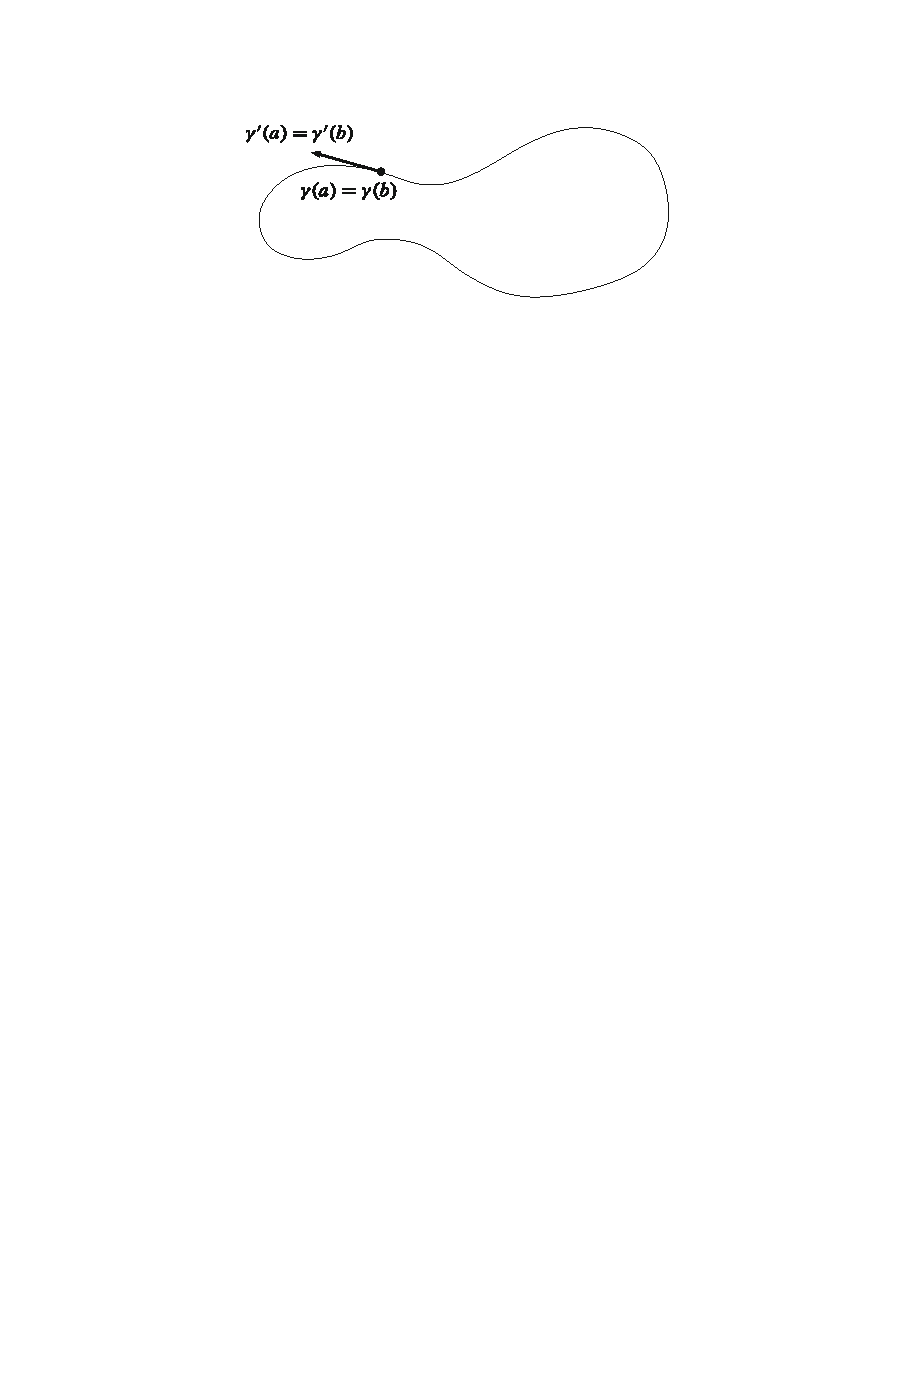
\includegraphics{pictures/closed-smooth-curve}
\caption{A closed curve with $\gamma'(a)=\gamma'(b)$.}
\end{figure}

If $\gamma$ is smooth (or at least continuously differentiable), we define a \textbf{tangent angle function for $\bm{\gamma}$} to be a continuous function $\theta:[a,b]\to\R$ 
such that $T(t)=(\cos\theta(t),\sin\theta(t))$ for all $t\in[a,b]$. It follows from the theory of covering spaces that such a function exists: the map $p:\R\to S^1$ 
given by $p(t)=(\cos t,\sin t)$ is a smooth covering map, and the path-lifting property of covering maps ensures that there is a continuous function $\theta:[a,b]\to\R$ 
that satisfies $p(\theta(t))=T(t)$. By the unique lifting property, a lift is uniquely determined once its value at any single point is determined, and thus any two 
lifts differ by a constant integral multiple of $2\pi$.\par
If $\gamma$ is a continuously differentiable simple closed curve such that $\gamma'(a)=\gamma'(b)$, then $(\cos\theta(a),\sin\theta(a))=(\cos\theta(b),\sin\theta(b))$, 
so $\theta(b)-\theta(a)$ must be an integral multiple of $2\pi$. For such a curve, we define the \textbf{rotation index} of $\gamma$ to be the following integer:
\[\rho(\gamma)=\frac{1}{2\pi}(\theta(b)-\theta(a)).\]
where $\theta$ is any tangent angle function for $\gamma$. For any other choice of tangent angle function, $\gamma(a)$ and $\gamma(b)$ would change by addition of the 
same constant, so the rotation index is independent of the choice of $\theta$.
We would also like to extend the definition of the rotation index to certain piecewise regular closed curves. For this purpose, we have to take into account the "jumps" 
in the tangent angle function at corners. To do so, suppose $\gamma:[a,b]\to\R^2$ is an admissible simple closed curve, and let $(a_0,\dots,a_k)$ be an admissible 
partition of $[a,b]$. The points $\gamma(a_i)$ are called the \textbf{vertices} of $\gamma$, and the curve segments $\gamma|_{[a_{i-1},a_i]}$ are called its \textbf{edges} or 
\textbf{sides}.\par
At each vertex  $\gamma(a_i)$, recall that $\gamma$ has left-hand and right-hand velocity vectors denoted by $\gamma'(a_i^{-})$ and $\gamma'(a_i^{+})$, respectively; 
let $T(a_i^{-})$ and $T(a_i^{+})$ denote the corresponding unit vectors. We classify each vertex into one of three categories:
\begin{itemize}
\item If $T(a_i^{-})\neq\pm T(a_i^{+})$, then $\gamma(a_i)$ is an \textbf{ordinary vertex}.
\item If $T(a_i^{-}=T(a_i^{+})$, then $\gamma(a_i)$ is an \textbf{flat vertex}.
\item If $T(a_i^{-})=-T(a_i^{+})$, then $\gamma(a_i)$ is a \textbf{cusp vertex}.
\end{itemize}
At each ordinary vertex, define the \textbf{exterior angle at $\bm{\gamma(a_i)}$} to be the oriented measure $\eps_i$ of the angle from $T(a_i^{-})$ to $T(a_i^{+})$, 
chosen to be in the interval $(-\pi,\pi)$, with a positive sign if $(T(a_i^{-}),T(a_i^{+}))$ is an oriented basis for $\R^2$, and a negative sign otherwise. At a flat 
vertex, the exterior angle is defined to be zero. At a cusp vertex, there is no simple way to choose unambiguously between $\pi$ and $-\pi$, so we leave the exterior 
angle undefined. The vertex $\gamma(a)=\gamma(b)$ is handled in the same way, with $T(b)$ and $T(a)$ playing the roles of $T(a^{-})$ and $T(a^{+})$, respectively. 
If $\gamma(a_i)$ is an ordinary or a flat vertex, the \textbf{interior angle at $\bm{\gamma(a_i)}$} is defined to be $\theta_i=\pi-\eps_i$; our conventions ensure that 
$0<\theta_i<2\pi$.
\begin{figure}[htbp]
\centering
\begin{minipage}[b]{200pt}
\centering
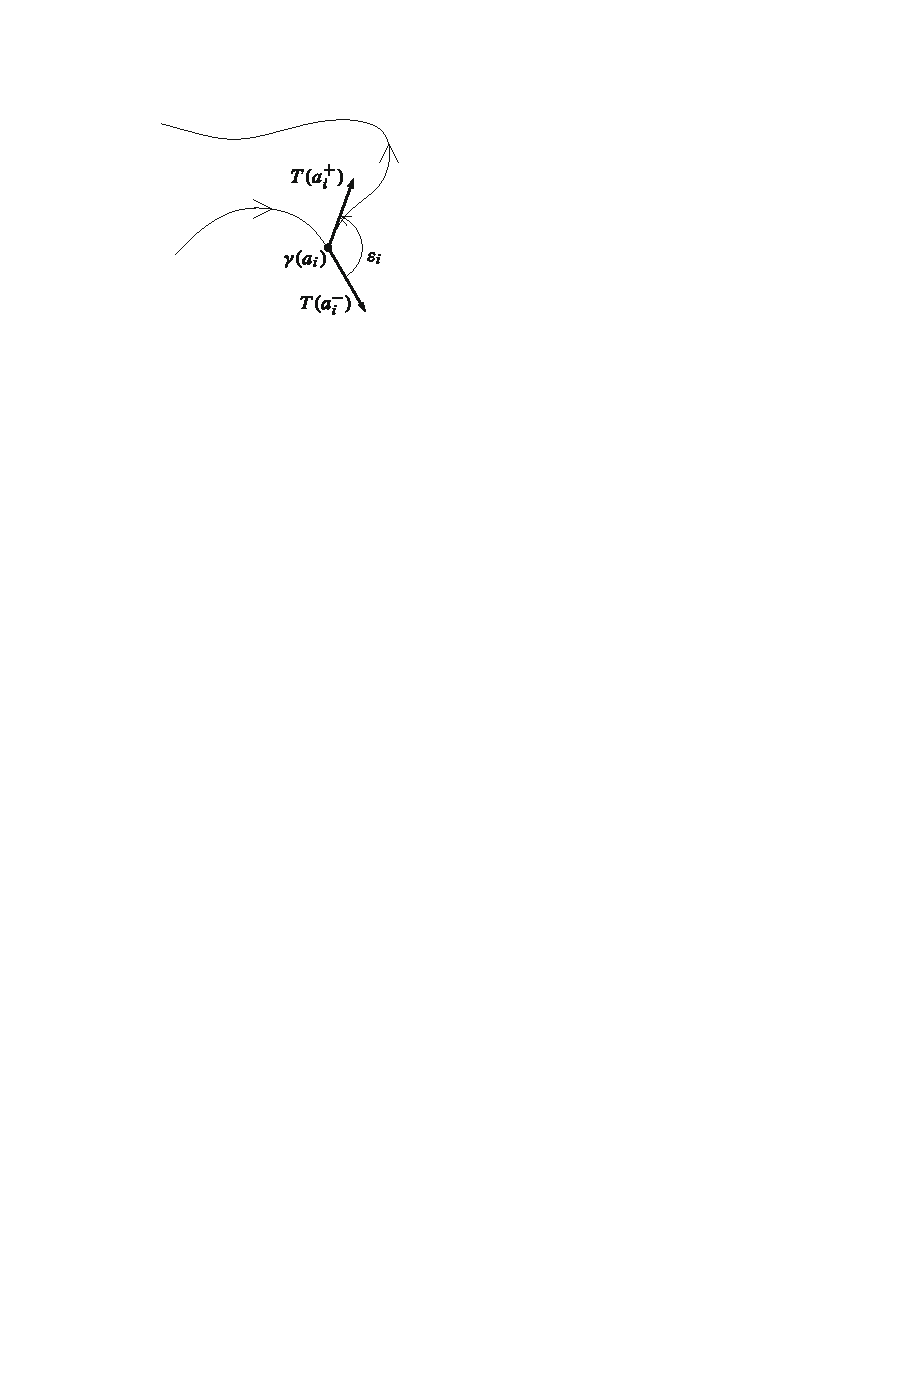
\includegraphics{pictures/exterior-angle}
\caption{An exterior angle.}
\end{minipage}
\hspace{20pt}
\begin{minipage}[b]{200pt}
\centering
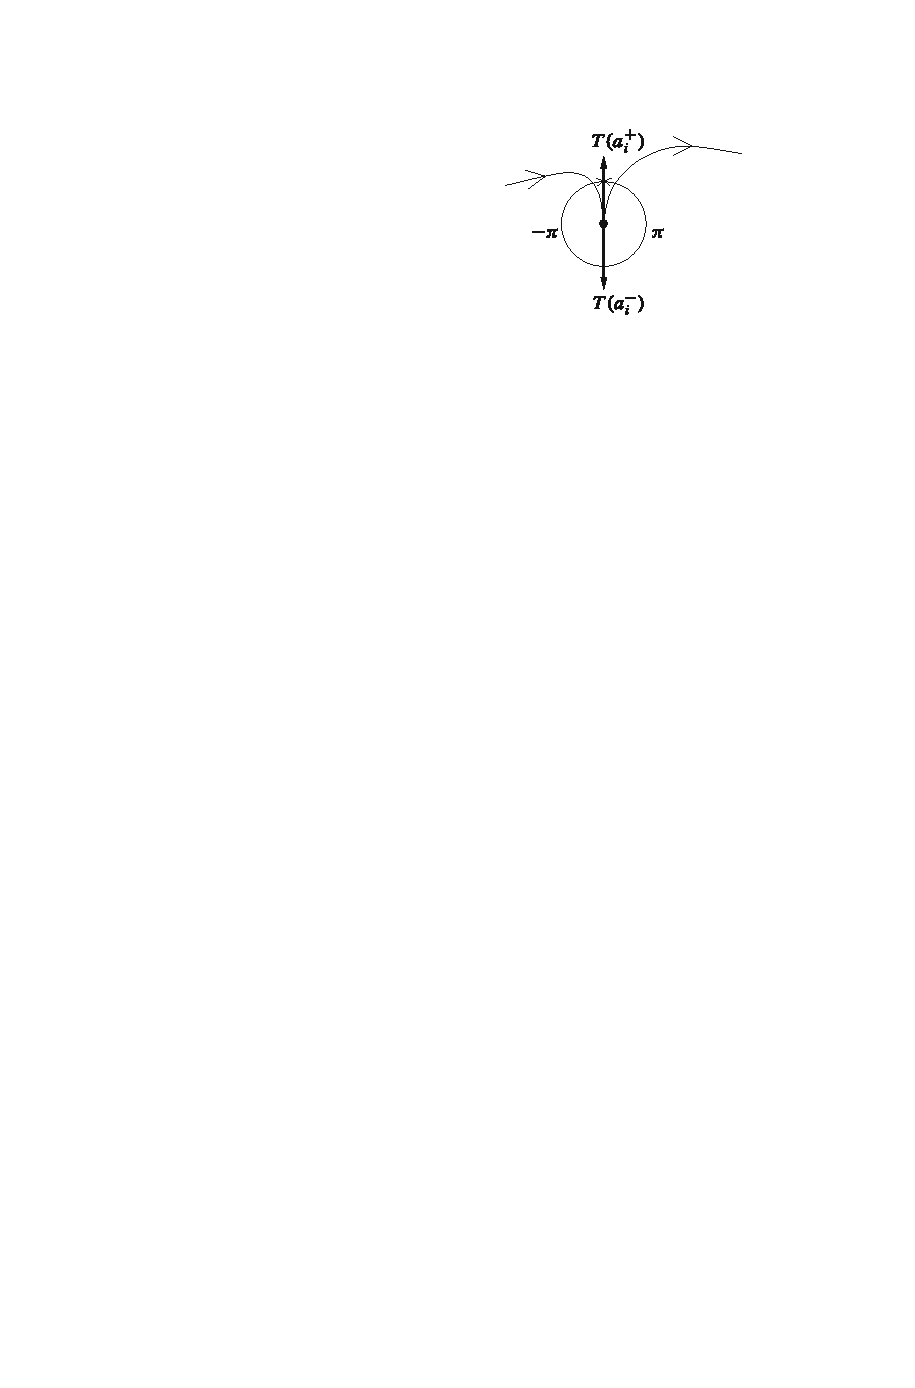
\includegraphics{pictures/cusp-vertex}
\caption{A cusp vertex.}
\end{minipage}
\end{figure}

The curves we wish to consider are of the following type: a \textbf{curved polygon} in the plane is an admissible simple closed curve without cusp vertices, whose 
image is the boundary of a precompact open set $\Omega\sub\R^2$. The set $\Omega$ is called the interior of $\gamma$ (not to be confused with the topological interior 
of its image as a subset of $\R^2$, which is the empty set).\par
Suppose $\gamma:[a,b]\to\R^2$ is a curved polygon. If $\gamma$ is parametrized so that at smooth points, $\gamma'$ is positively oriented with respect to the 
induced orientation on $\partial\Omega$ in the sense of Stokes's theorem, we say that $\gamma$ is \textbf{positively oriented}. Intuitively, this means that $\gamma$ 
is parametrized in the counterclockwise direction, or that $\Omega$ is always to the left of $\gamma$.
\begin{figure}[htbp]
\centering
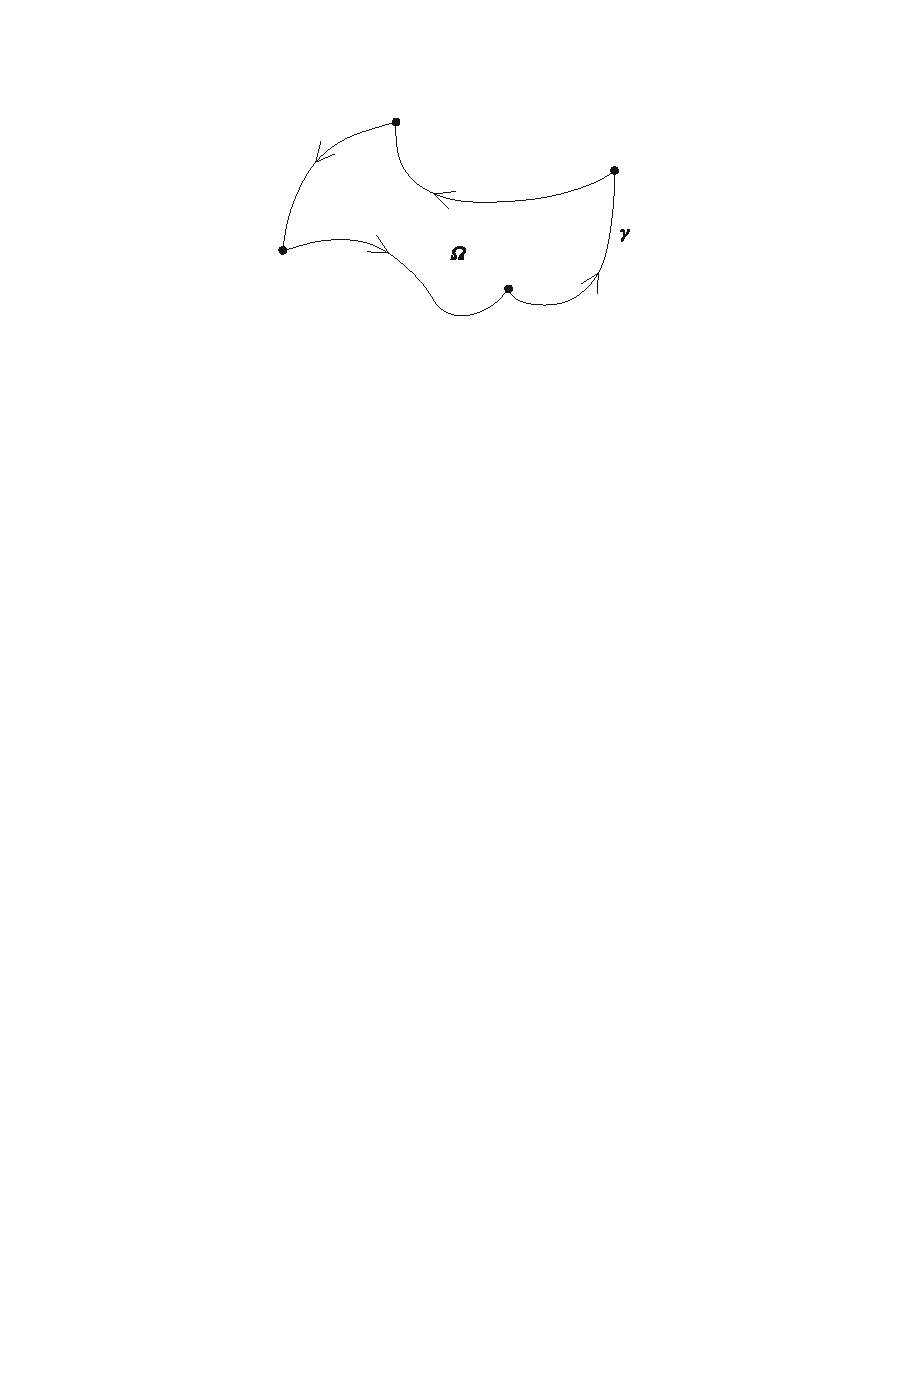
\includegraphics{pictures/oriented-polygon}
\caption{A positively oriented curved polygon.}
\end{figure}

We define a \textbf{tangent angle function for a curved polygon $\bm{\gamma}$} to be a piecewise continuous function $\theta:[a,b]\to\R$ that satisfies $T(t)=(\cos\theta(t),\sin\theta(t))$ 
at each point $t$ where $\gamma$ is smooth, that is continuous from the right at each $a_i$ with
\begin{align}\label{curved polygon tangent angle function-1}
\theta(a_i)=\lim_{t\to a_i^{-}}\theta(t)+\eps_i,
\end{align}
and that satisfies
\begin{align}\label{curved polygon tangent angle function-2}
\theta(b)=\lim_{t\to b}\theta(t)+\eps_k,
\end{align}
where $\eps_k$ is the exterior angle at $\gamma(b)$. Such a function always exists: start by defining $\theta(t)$ for $t\in[a,a_1)$ to be any lift of $T$ on that 
interval; then on $[a_1,a_2)$ define $\theta(t)$ to be the unique lift that satisfies $(\ref{curved polygon tangent angle function-1})$, and continue by induction, ending 
with $\gamma(b)$ defined by $(\ref{curved polygon tangent angle function-2})$.
\begin{figure}[htbp]
\centering
\begin{minipage}[b]{200pt}
\centering
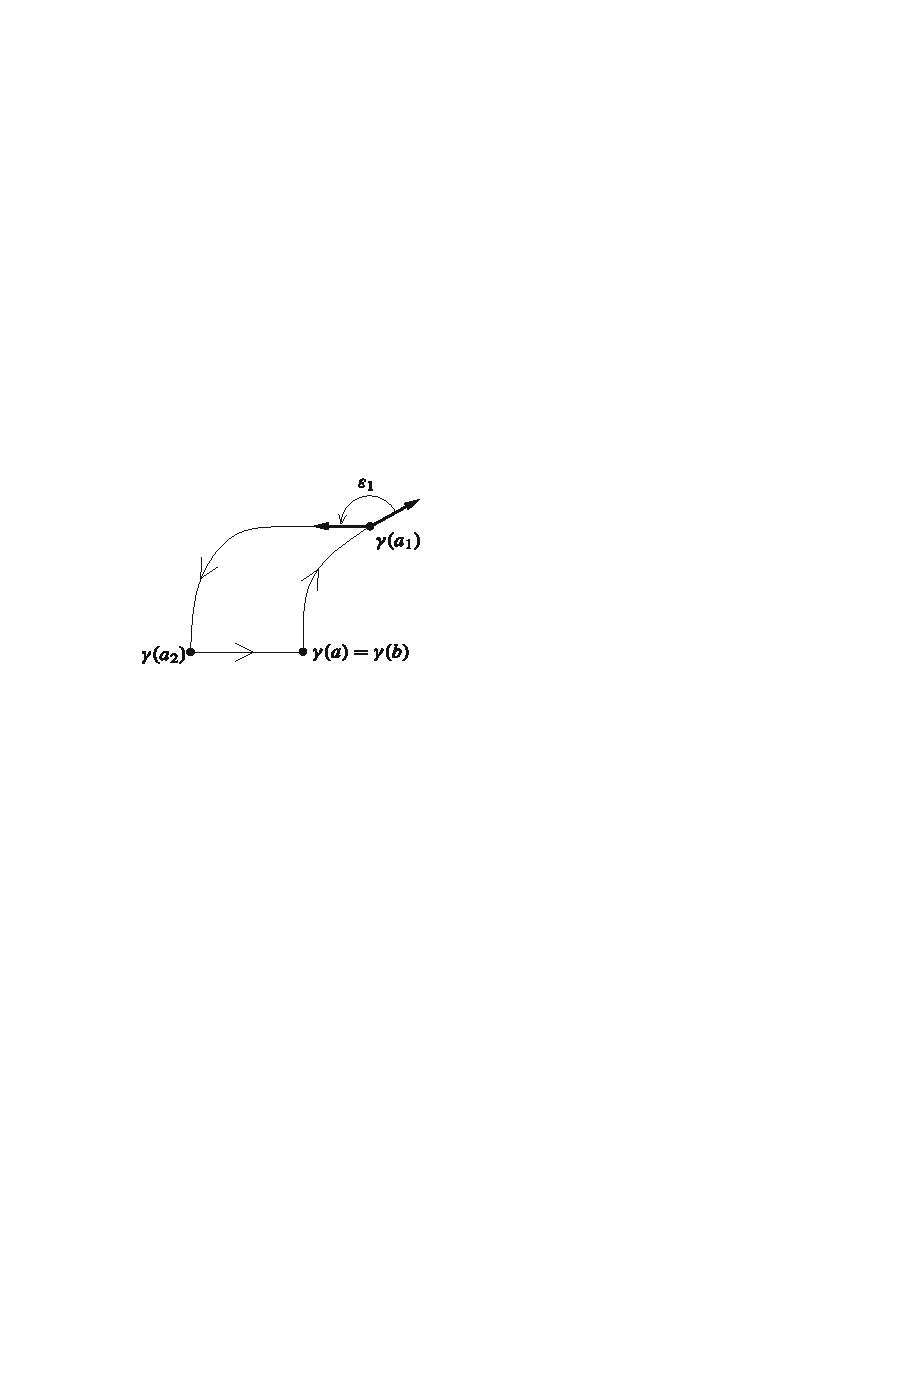
\includegraphics{pictures/tangent-angle}
\caption{Tangent angle at a vertex.}
\end{minipage}
\hspace{20pt}
\begin{minipage}[b]{200pt}
\centering
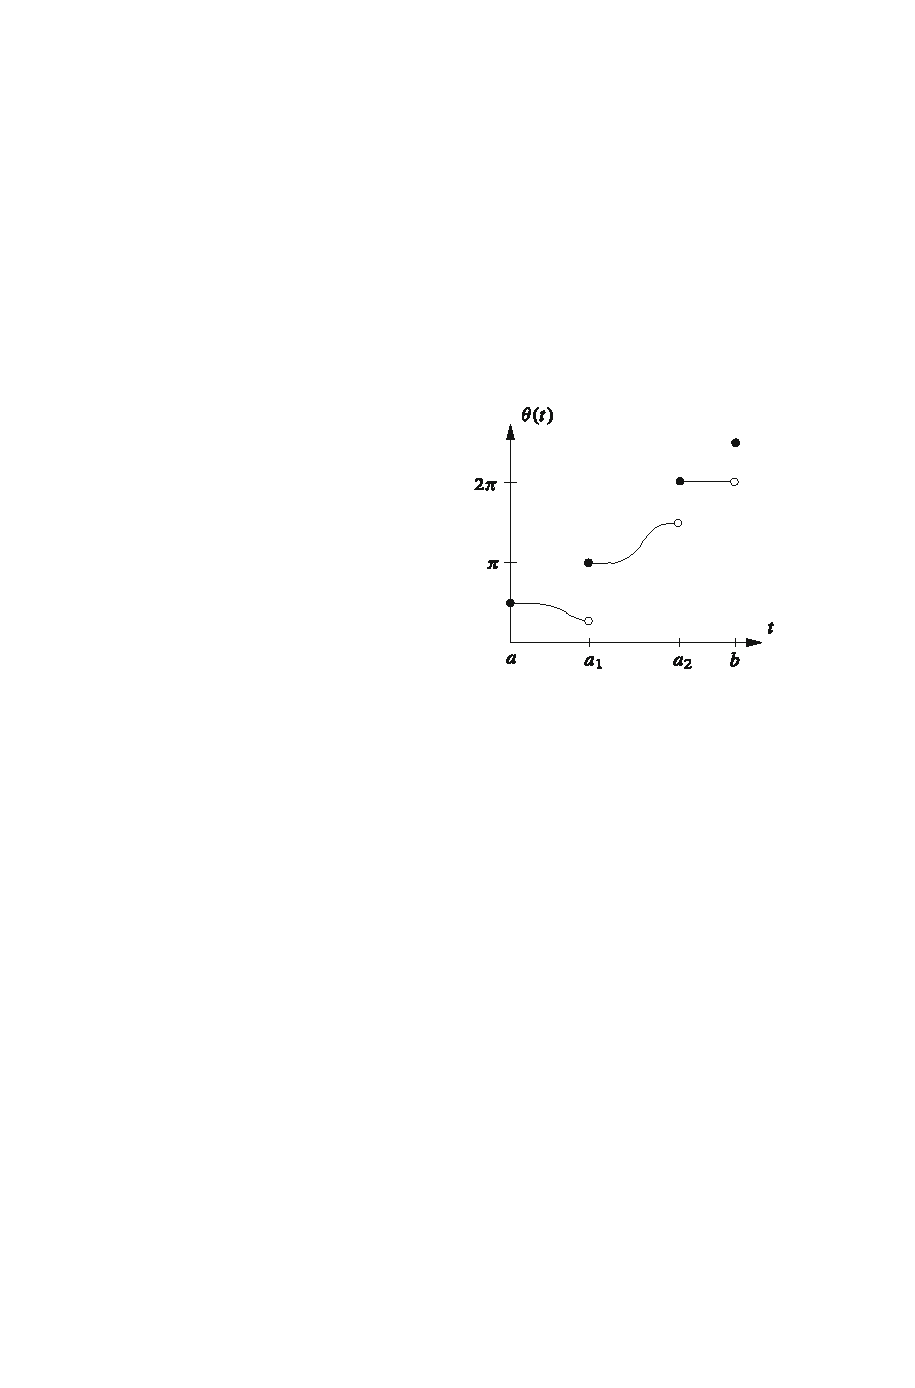
\includegraphics{pictures/tangent-angle-function}
\caption{Tangent angle function.}
\end{minipage}
\end{figure}

Once again, the difference between any two such functions is a constant integral multiple 
of $2\pi$. We define the rotation index of $\gamma$ to be
\[\rho(\gamma)=\frac{1}{2\pi}(\theta(b)-\theta(a)),\]
just as in the smooth case. As before, $\rho(\gamma)$ is an integer, because the definition ensures that $(\cos\theta(b),\sin\theta(b))=(\cos\theta(a),\sin\theta(a))$.
\begin{theorem}[\textbf{Rotation Index Theorem}]
The rotation index of a positively oriented curved polygon in the plane is $+1$.
\end{theorem}
\begin{proof}
Let $\gamma:[a,b]\to\R^2$ be such a curved polygon. Assume first that all the vertices of $\gamma$ are flat. This means, in particular, that $\gamma'$ is continuous and $\gamma'(a)=\gamma'(b)$. 
Since $\gamma(a)=\gamma(b)$, we can extend $\gamma$ to a continuous map from $\R$ to $\R^2$ by requiring it to be periodic of period $b-a$, and our hypothesis $\gamma'(a)=\gamma'(b)$ 
guarantees that the extended map still has continuous first derivatives. Define $T(t)=\gamma'(t)/|\gamma'(t)|$ as before.\par
Let $\theta:\R\to S^1$ be any lift of $T:\R\to S^1$. Then $\theta|_{[a,b]}$ is a tangent angle function for $\gamma$, and thus $\theta(b)=\theta(a)+2\pi\rho(\gamma)$. If we set $\tilde{\theta}(t)=\theta(t+b-a)-2\pi\rho(\gamma)$, then
\[(\cos\hat{\theta}(t),\sin\hat{\theta}(t))=(\cos\theta(t+b-a),\sin\theta(t+b-a))=T(t+b-a)=T.\]
so $\tilde{\theta}$ is also a lift of $T$. Because $\tilde{\theta}(a)=\theta(a)$, it follows that $\tilde{\theta}\equiv\theta$, or in other words the following 
equation holds for all $t\in\R$:
\begin{align}\label{rotation index-1}
\theta(t+b-a)=\theta(t)+2\pi\rho(\gamma).
\end{align}
If $a_1$ is an arbitrary point in $[a,b]$ and $b_1=a_1+b-a$, then $\gamma|_{[a_1,b_1]}$ is also a positively oriented curved polygon with only flat vertices, and $\theta|_{[a_1,b_1]}$ 
is a tangent angle function for it. Note that $(\ref{rotation index-1})$ implies
\[\theta(b_1)-\theta(a_1)=\theta(a_1+b-a)-\theta(a_1)=\theta(a_1)+2\pi\rho(\gamma)-\theta(a_1)=2\pi\rho(\gamma).\]
so $\gamma|_{[a_1,b_1]}$ has the same rotation index as $\gamma|_{[a,b]}$. Thus we obtain the same result by restricting $\gamma$ to any closed interval of length $b-a$.
\begin{figure}[htbp]
\centering
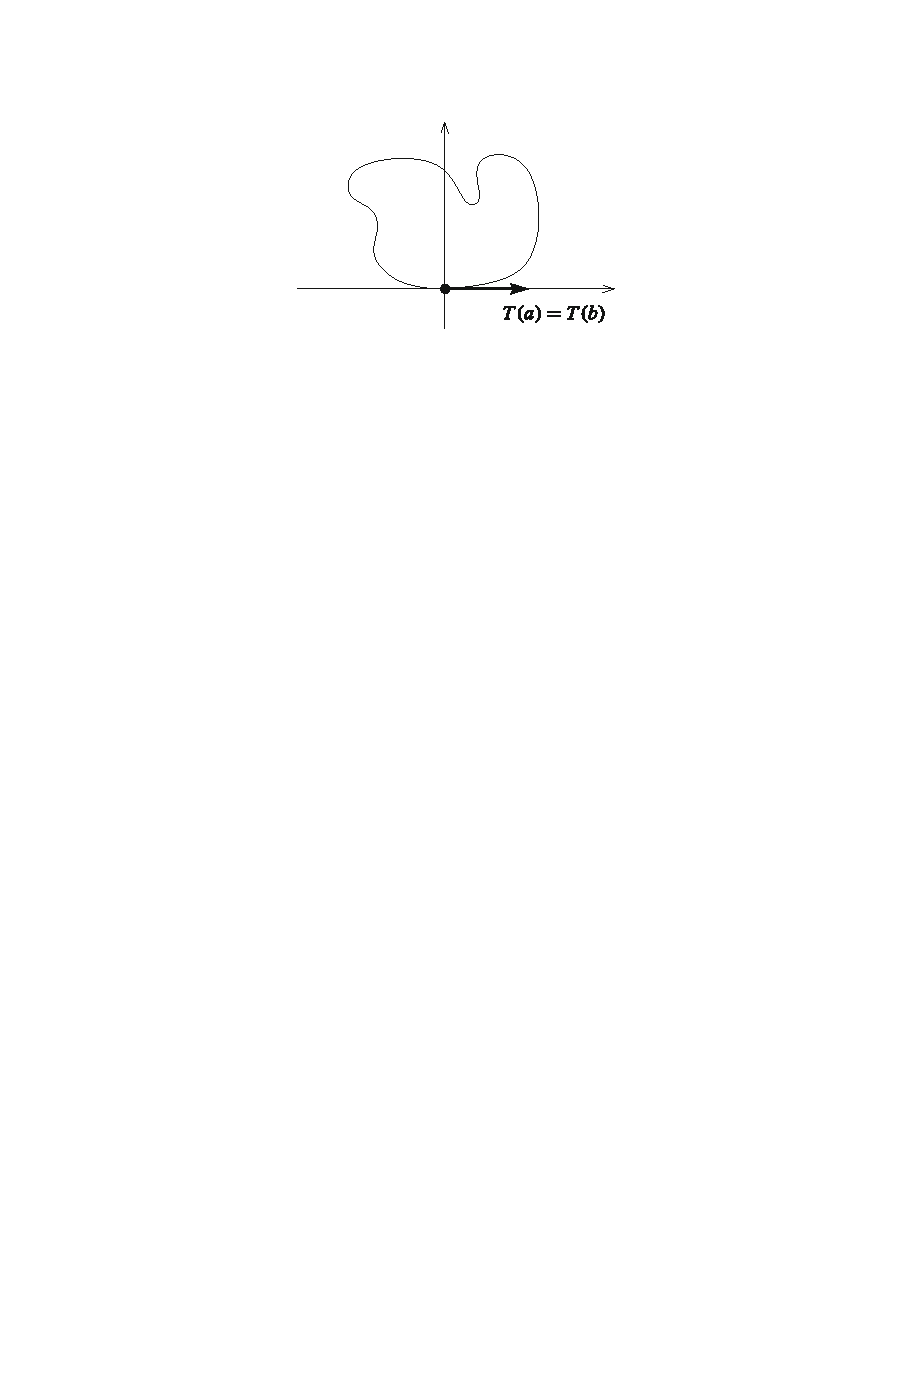
\includegraphics{pictures/rotation-index-theorem}
\caption{Changing the parameter interval and translating $\gamma(a)$ to the origin.}
\end{figure}

Using this freedom, we can assume that the parameter interval $[a,b]$ has been chosen so that the $y$-coordinate of $\gamma$ achieves its minimum at $t=a$. Moreover, by 
a translation in the $xy$-plane (which does not change $\gamma'$ or $\gamma$), we may as well assume that $\gamma(a)$ is the origin. With these adjustments, the image 
of $\gamma$ remains in the closed upper half-plane, and $T(a)=T(b)=(1,0)$. By adding a constant integral multiple of $2\pi$ to $\theta$ if necessary, we can also assume 
that $\theta(a)=0$.
\begin{figure}[htbp]
\centering
\begin{minipage}[b]{200pt}
\centering
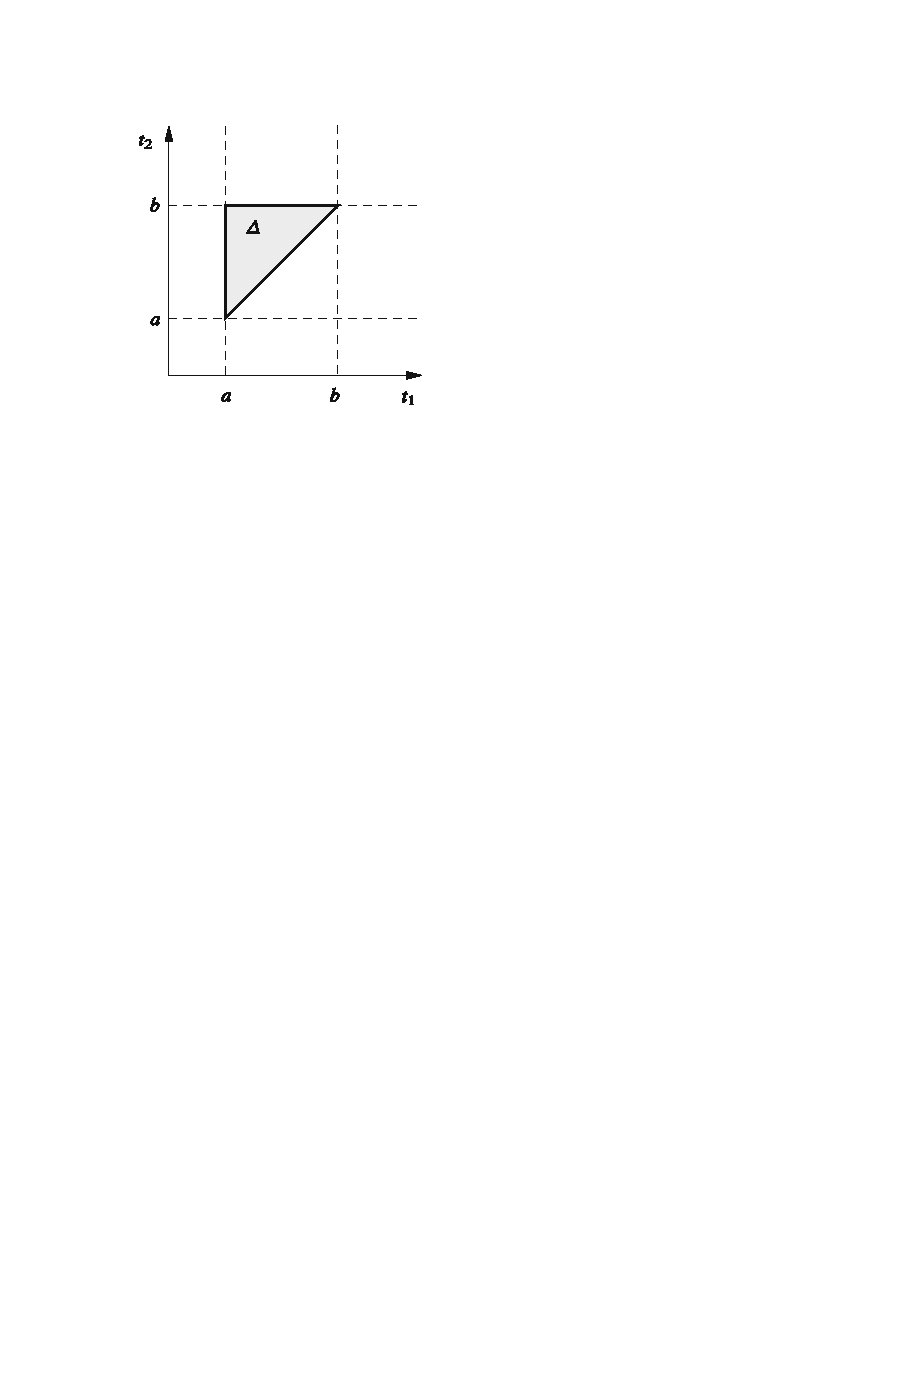
\includegraphics{pictures/rotation-index-domain.pdf}
\caption{The domain of $\varphi$.}
\end{minipage}
\hspace{20pt}
\begin{minipage}[b]{200pt}
\centering
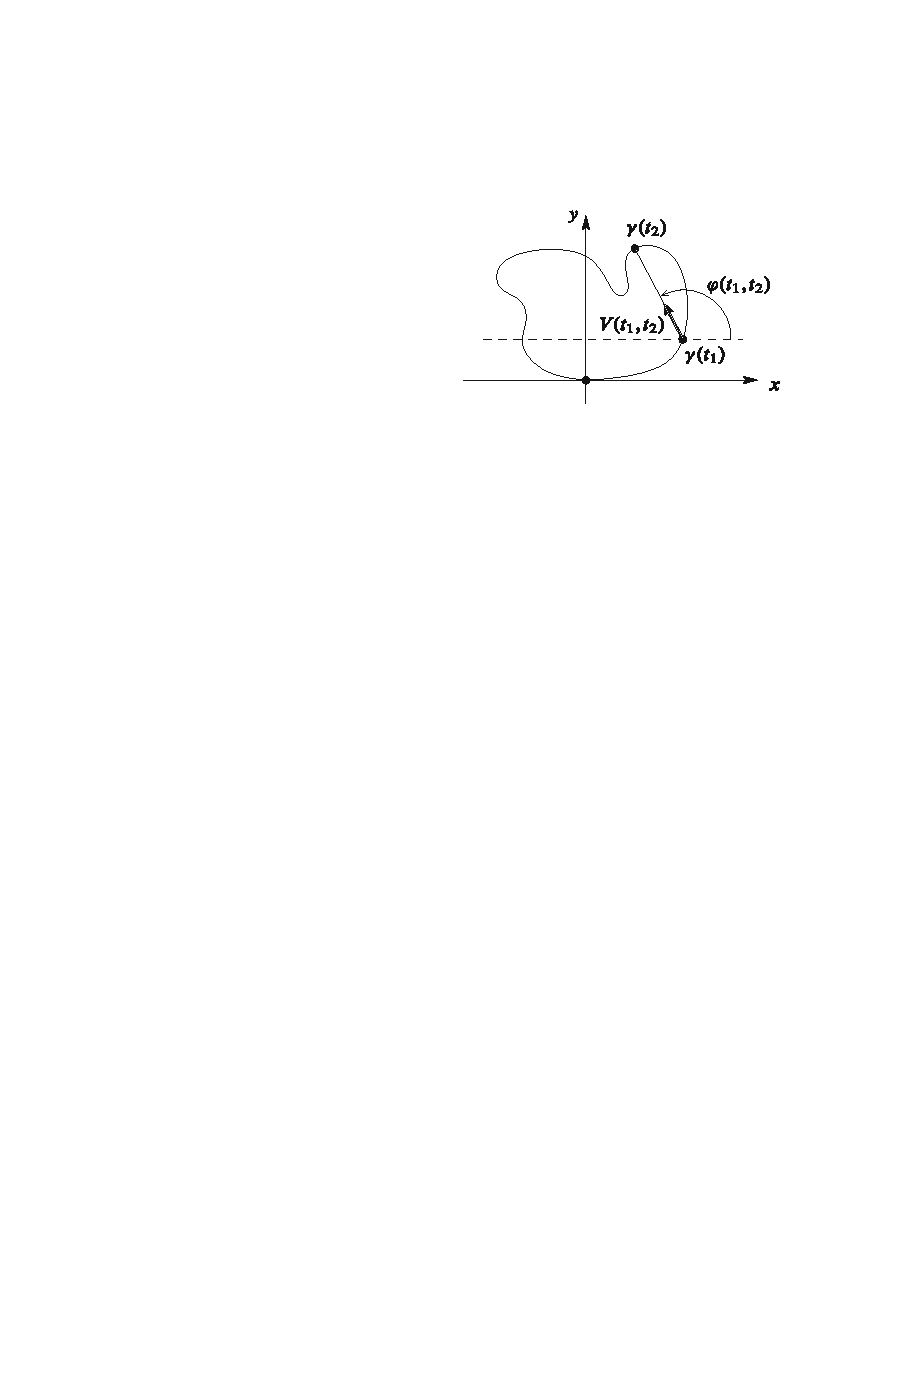
\includegraphics{pictures/secant-angle-function}
\caption{The secant angle function.}
\end{minipage}
\end{figure}

Next, we define a continuous \textbf{secant angle function}, denoted by $\varphi(t_1,t_2)$, representing the angle between the positive $x$-direction and the vector 
from $\gamma(t_1)$ to $\gamma(t_2)$. To be precise, let $\Delta\sub\R^2$ be the triangular region $\Delta=\{(t_1,t_2):a\leq t_1\leq t_2\leq b\}$, and define a map $V:\Delta\to S^1$ by
\[V(t_1,t_2)=\begin{cases}
\dfrac{\gamma(t_2)-\gamma(t_1)}{|\gamma(t_2)-\gamma(t_1)|},&t_1<t_2\text{ and }(t_1,t_2)\neq(a,b);\\
T(t_1),&t_1=t_2;\\
-T(b),&(t_1,t_2)=(a,b).
\end{cases}\]
The function $V$ is continuous at points where $t_1<t_2$ and $(t_1,t_2)\neq(a,b)$, because $\gamma$ is continuous and injective there. To see that it is continuous 
elsewhere, note that for $t_1<t_2$, the fundamental theorem of calculus gives
\[\gamma(t_2)-\gamma(t_1)=\int_{0}^{1}\frac{d}{ds}\gamma(t_1+s(t_2-t_1))ds=\int_{0}^{1}\gamma'(t_1+s(t_2-t_1))(t_2-t_1)ds.\]
and thus
\[\Big|\frac{\gamma(t_2)-\gamma(t_1)}{t_2-t_1}-\gamma'(t)\Big|\leq\int_{0}^{1}|\gamma'(t_1+s(t_2-t_1))-\gamma'(t)|ds.\]
Because $\gamma'$ is uniformly continuous on the compact set $[a,b]$, this last expression can be made as small as desired by taking $(t_1,t_2)$ close to $(t,t)$. It 
follows that
\[\lim_{(t_1,t_2)\to(t,t)\atop t_1<t_2}\frac{\gamma(t_2)-\gamma(t_1)}{t_2-t_1}=\gamma'(t),\]
and therefore
\[\lim_{(t_1,t_2)\to(t,t)\atop t_1<t_2}V(t_1,t_2)=\lim_{(t_1,t_2)\to(t,t)\atop t_1<t_2}\frac{\gamma(t_2)-\gamma(t_1)}{|\gamma(t_2)-\gamma(t_1)|}=\frac{\gamma'(t)}{\gamma'(t)|}=T(t)=V(t,t).\]
Similarly, because $T$ is continuous,
\[\lim_{(t_1,t_2)\to(t,t)\atop t_1=t_2}V(t_1,t_2)=\lim_{t_1\to t}T(t_1)=T(t)=V(t,t).\]
It follows that $V$ is continuous at $(t,t)$.\par
To prove that $V$ is continuous at $(a,b)$, recall that we have extended $\gamma$ to be periodic of period $b-a$. The argument above gives
\begin{align*}
\lim_{(t_1,t_2)\to(a,b)\atop t_1<t_2}V(t_1,t_2)&=\lim_{(t_1,t_2)\to(a,b)\atop t_1<t_2}\frac{\gamma(t_2)-\gamma(t_1+b-a)}{|\gamma(t_2)-\gamma(t_1+b-a)|}\\
&=\lim_{(s_1,s_2)\to(b,b)\atop s_1>_2}\frac{\gamma(s_2)-\gamma(s_1)}{|\gamma(s_2)-\gamma(s_1)|}=-T(b)=V(a,b).
\end{align*}
Thus $V$ is continuous.\par
Since $\Delta$ is simply connected, the map $V:\Delta\to S^1$ has a continuous lift $\varphi:\Delta\to\R$, which is unique if we require $\varphi(a,a)=0$. This is our 
secant angle function.\par
We can express the rotation index in terms of the secant angle function as follows:
\[\rho(\gamma)=\frac{1}{2\pi}(\theta(b)-\theta(a))=\frac{1}{2\pi}(\varphi(b,b)-\varphi(a,a))=\frac{1}{2\pi}\varphi(b,b).\]
Observe that along the side of $\Delta$ where $t_1=a$ and $t_2\in[a,b]$, the vector $V(a,t_2)$ has its tail at the origin and its head in the upper half-plane. Since we stipulate that $\varphi(a,a)=0$, we must have $\varphi(a,t_2)\in[0,\pi]$ on this segment. By continuity, therefore, $\varphi(a,b)=\pi$ (since $\varphi(a,b)$ represents the tangent angle of $-T(b)=(-1,0)$). Similarly, on the side where $t_2=b$, the vector $V(t_1,b)$ has its head at the origin and its tail in the upper half-plane, so $\varphi(t_1,b)\in[\pi,2\pi]$ Therefore, since $\varphi(b,b)$ represents the tangent angle of $T(b)=(1,0)$, we must have $\varphi(b,b)=2\pi$ and therefore $\rho(\gamma)=1$. This completes the proof for the case in which $\gamma'$ is continuous.\par
Now suppose $\gamma$ has one or more ordinary vertices. It suffices to show there is a curve with a continuous velocity vector field that has the same rotation index as $\gamma$. We will construct such a curve by "rounding the corners" of $\gamma$. It will simplify the proof somewhat if we choose the parameter interval $[a,b]$ so that $\gamma(a)=\gamma(b)$ is not one of the ordinary vertices.
\begin{figure}[H]
\centering
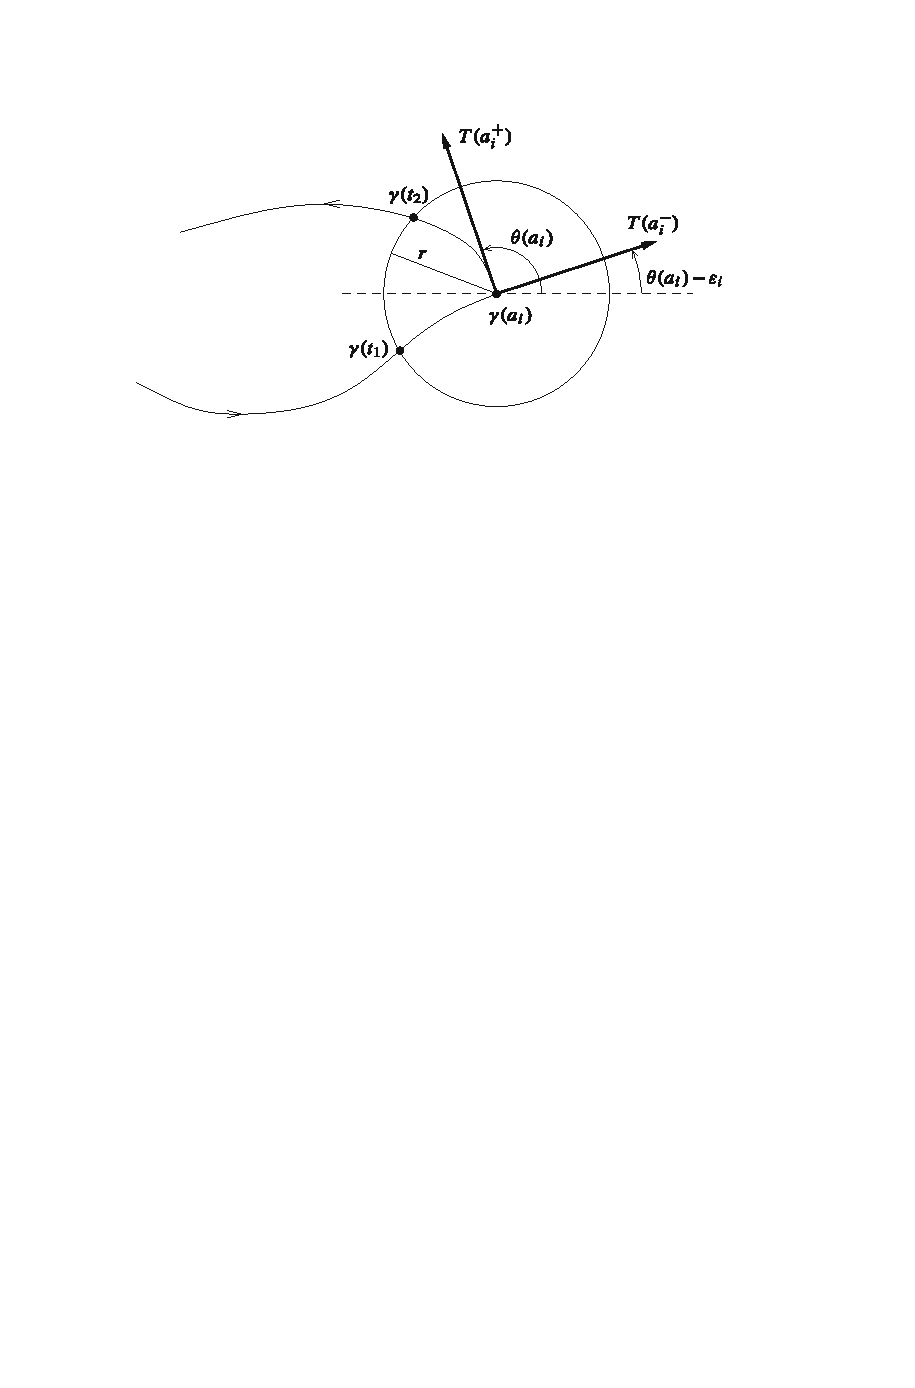
\includegraphics[width=0.5\textwidth]{pictures/isolating-corner}
\caption{Isolating the change in the tangent angle at a vertex.}
\end{figure}

Let $\gamma(a_i)$ be any ordinary vertex, let $\eps_i$ be its exterior angle, and let $\alpha$ be a positive number less than $(\pi-|\eps_i|)/2$. Recall that $\gamma$ 
is continuous from the right at $a_i$ and $\lim_{t\to a_i^{-}}\theta(t)=\theta(a_i)-\eps_i$. Therefore, we can choose $\delta$ small enough that $|\theta(t)-\theta(a_i)-\eps_i|<\alpha$ 
when $t\in(a_i-\delta,a_i)$, and $|\theta(t)-\theta(a_i)|<\alpha$ when $t\in(a_i,a_i+\delta)$.\par
The image under $\gamma$of $[a,b]\setminus(a_i-\delta,a_i+\delta)$ is a compact set that does not contain $\gamma(a_i)$, so we can choose $r$ small enough that $\gamma$ does not enter $\widebar{B_r(\gamma(a_i)}$ except when $t\in(a_i-\delta,a_i+\delta)$. Let $t_1\in(a_i-\delta,a_i)$ denote a time when $\gamma$ enters $\widebar{B_r(\gamma(a_i))}$, and $t_2\in(a_i,a_i+\delta)$ a time when it leaves. By our choice of $\delta$, the total change in $\theta(t)$ is not more than $\alpha$ when $t\in[t_1,a_i)$, and again not more than $\alpha$ when $t\in(a_i,t_2]$. Therefore, the total change $\Delta\theta$ in $\gamma(t)$ during the time interval $[t_1,t_2]$ is between $\eps-2\alpha$ and $\eps+2\alpha$ which implies $-\pi<\Delta\theta<\pi$.
\begin{figure}[H]
\centering
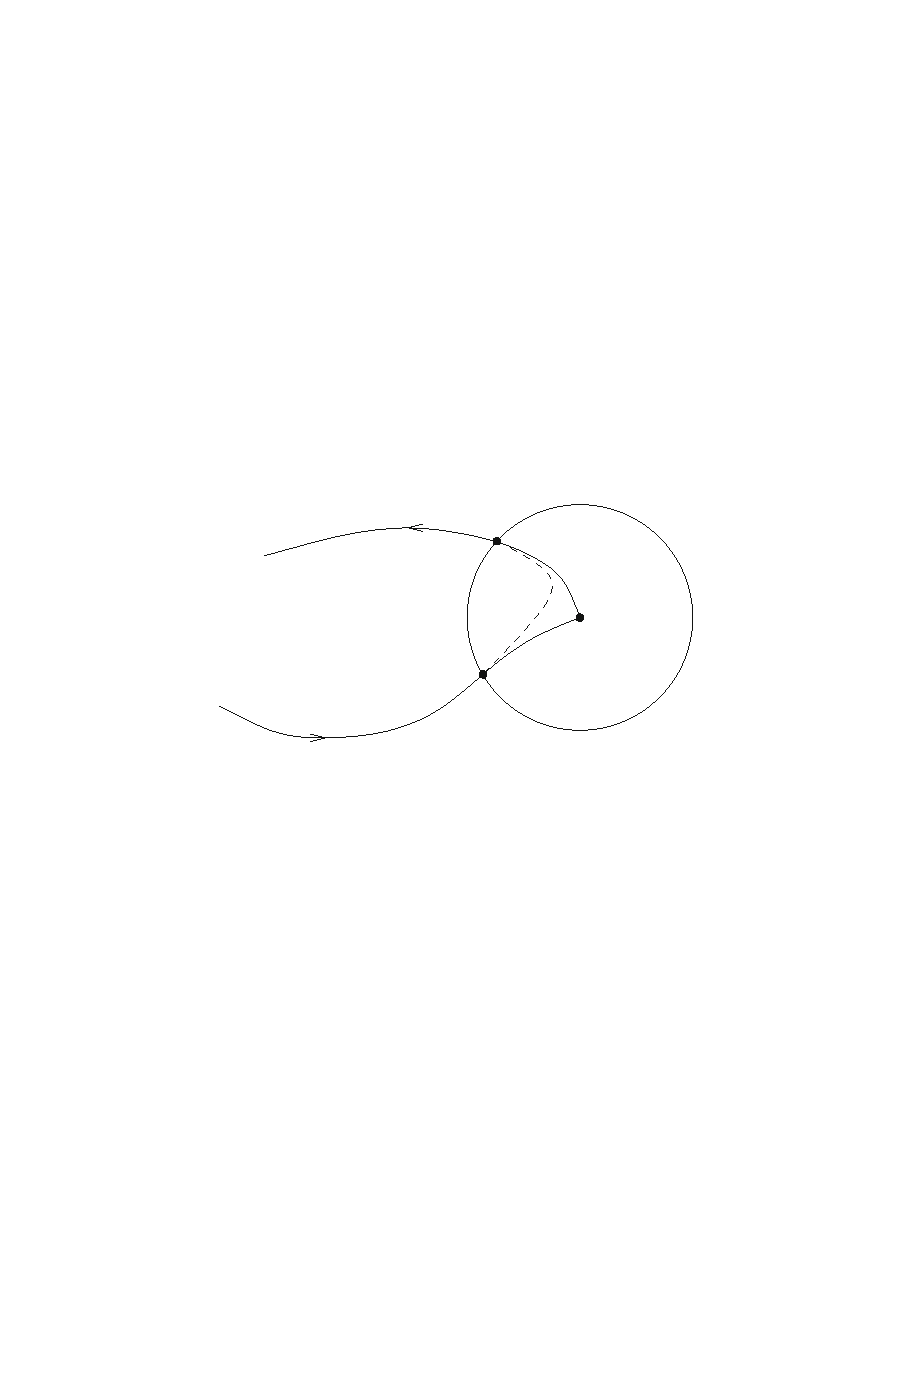
\includegraphics[width=0.4\textwidth]{pictures/rounding-corner}
\caption{Rounding a corner.}
\end{figure}

Now we simply replace $\gamma|_{[t_1,t_2]}$ with a smooth curve segment $\sigma$ that has the same velocity as $\gamma$ at $\gamma(t_1)$ and $\gamma(t_2)$, and whose tangent angle increases or decreases monotonically from $\gamma(t_1)$ to $\gamma(t_2)$; an arc of a hyperbola will do. Since the change in tangent angle of $\sigma$ is between $-\pi$ and $\pi$ and represents the angle between $T(t_1)$ and $T(t_2)$, it must be exactly $\Delta\theta$. Repeating this process for each vertex, we obtain a new curved polygon with a continuous velocity vector field whose rotation index is the same as that of $\gamma$, thus proving the theorem.
\end{proof}
\subsection{The Gauss-Bonnet formula}
We now direct our attention to the case of an oriented Riemannian $2$-manifold $(M,g)$. In this setting, an admissible simple closed curve $\gamma:[a,b]\to M$ is called a 
\textbf{curved polygon in $\bm{M}$} if the image of $\gamma$ is the boundary of a precompact open set $\Omega\sub M$, and there is an oriented smooth coordinate disk 
containing $\widebar{\Omega}$ under whose image $\gamma$ is a curved polygon in the plane. As in the planar case, we call $\Omega$ the \textbf{interior of $\bm{\gamma}$}. 
A curved polygon whose edges are all geodesic segments is called a \textbf{geodesic polygon}.
\begin{figure}[htbp]
\centering
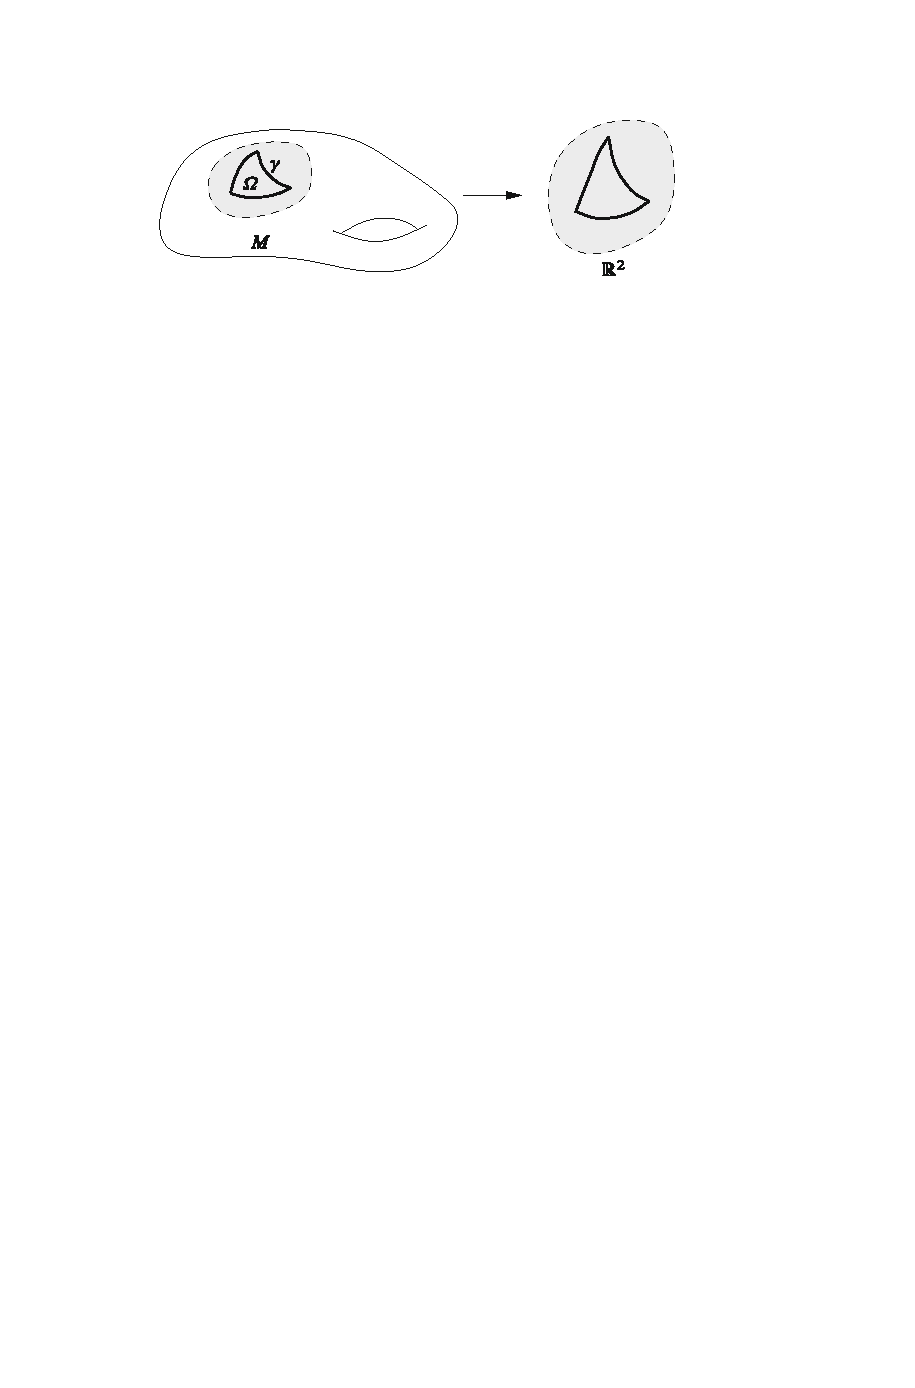
\includegraphics{pictures/curved-polygon-surface}
\caption{A curved polygon on a surface.}
\end{figure}

For a curved polygon $\gamma$ in $M$, our previous definitions go through almost unchanged. We say that $\gamma$ is \textbf{positively oriented} if it is parametrized in 
the direction of its Stokes orientation as the boundary of $\Omega$. On each smooth segment of $\gamma$, we define the \textbf{unit tangent vector field} 
$T(t)=\gamma'(t)/|\gamma'(t)|$. If $\gamma(a_i)$ is an ordinary or flat vertex, we define the \textbf{exterior angle of $\bm{\gamma}$} at $\gamma(a_i)$ as the oriented 
measure $\eps_i$ of the angle from $T(a_i^{-})$ to $T(a_i^{+})$ with respect to the $g$-inner product and the given orientation of $M$; explicitly, this is
\begin{align}\label{Riemann exterior angle}
\eps_i=\frac{dV_g(T(a_i^{-}),T(a_i^{+}))}{|dV_g(T(a_i^{-}),T(a_i^{+}))|}\arccos\langle T(a_i^{-}),T(a_i^{+})\rangle.
\end{align}
The corresponding \textbf{interior angle of $\bm{\gamma}$ at $\bm{\gamma(a_i)}$} is $\theta_i=\pi-\eps_i$. Exterior and interior angles at $\gamma(a)=\gamma(b)$ are 
defined similarly.\par
We need a version of the rotation index theorem for curved polygons in $M$. Suppose $\gamma:[a,b]\to M$ is a curved polygon and $\Omega$ is its interior, and let $(U,\varphi)$ be an oriented smooth chart such that $U$ contains $\widebar{\Omega}$. Using the coordinate map $\varphi$ to transfer $\gamma$, $\Omega$, and $g$ to the plane, we may as well assume that $g$ is a metric on some open subset $\widehat{U}\sub\R^2$, and $\gamma$ is a curved polygon in $\widehat{U}$. Let $(E_1,E_2)$ be the oriented orthonormal frame for $g$ obtained by applying the Gram-Schmidt algorithm to $(\partial_x,\partial_y)$, so that $E_1$ is a positive scalar multiple of $\partial_x$ everywhere in $\widehat{U}$.\par
We define a \textbf{tangent angle function for $\bm{\gamma}$} to be a piecewise continuous function $\theta:[a,b]\to\R$ that satisfies
\[T(t)=\cos\theta(t) E_1|_{\gamma(t)}+\sin\theta(t)E_2|_{\gamma(t)}.\]
at each $t$ where $\gamma'$ is continuous, and that is continuous from the right and satisfies $(\ref{curved polygon tangent angle function-2})$ and 
$(\ref{curved polygon tangent angle function-2})$ at vertices. The existence of such a function follows as in the planar case, using the fact that
\begin{align*}
T(t)=u_1E_1|_{\gamma(t)}+u_2E_2|_{\gamma(t)}
\end{align*}
for a pair of piecewise continuous functions $u_1,u_2:[a,b]\to\R$ that can be regarded as the coordinate functions of a map $(u_1,u_2):[a,b]\to S^1$ because $T$ has unit 
length.\par
The \textbf{rotation index of $\bm{\gamma}$} is $(\theta(b)-\theta(a))/2\pi$. Because of the role played by the specific frame $(E_1,E_2)$ in the definition, it is not obvious that 
the rotation index has any coordinate-independent meaning; however, the following easy consequence of the rotation index theorem shows that it does not depend on the 
choice of coordinates.
\begin{lemma}
If $M$ is an oriented Riemannian $2$-manifold, the rotation index of every positively oriented curved polygon in $M$ is $+1$.
\end{lemma}
\begin{proof}
If we use the given oriented coordinate chart to regard $\gamma$ as a curved polygon in the plane, we can compute its tangent angle function either with respect to $g$ or 
with respect to the Euclidean metric $\widebar{g}$. In either case, $\rho(\gamma)$ is an integer because $\theta(a)$ and $\theta(b)$ both represent the angle between the 
same two vectors, calculated with respect to some inner product. Now for $0\leq s\leq 1$, let $g_s=sg+(1-s)\widebar{g}$. By the same reasoning, the rotation index 
$\rho_{g_s}(\gamma)$ with respect to $g_s$ is also an integer for each $s$, so the function $f(s)=\rho_{g_s}(\gamma)$ is integer-valued.\par
In fact, the function $f$ is continuous in $s$, as can be deduced easily from the following observations: $(1)$ Our preferred $g_s$-orthonormal frame $(E^{(s)}_1,E^{(s)}_2)$ 
depends continuously on $s$, as can be seen from the formulas of the Gram–Schmidt algorithm. $(2)$ On every interval $[a_{i-1},a_i]$ where $\gamma$ is smooth, the functions 
$u_1$ and $u_2$ satisfying the $g_s$-analogue of $()$ can be expressed as $u_j(t,s)=\langle T_s(t),E_j^{(s)|_{\gamma(t)}}\rangle_{g_s}$, where $T_s(t)=\gamma'(t)/|\gamma'(t)|_{g_s}$. 
Thus $u_1$ and $u_2$ depend continuously on $(t,s)\in[a_{i-1},a_i]\times[0,1]$, so the function $(u_1,u_2):[a_{i-1},a_i]\times[0,1]\to S^1$ has a continuous lift $\theta:[a_{i-1},a_i]\times[0,1]\to\R$, 
uniquely determined by its value at one point. $(3)$ At each vertex, it follows from formula $(\ref{Riemann exterior angle})$ that the exterior angle depends continuously 
on $g_s$.\par
Because $f$ is continuous and integer-valued, it follows that $\rho(\gamma)=f(1)=f(0)=\rho_{\widebar{g}}(\gamma)=1$, which was to be proved.
\end{proof}
\begin{figure}[htbp]
\centering
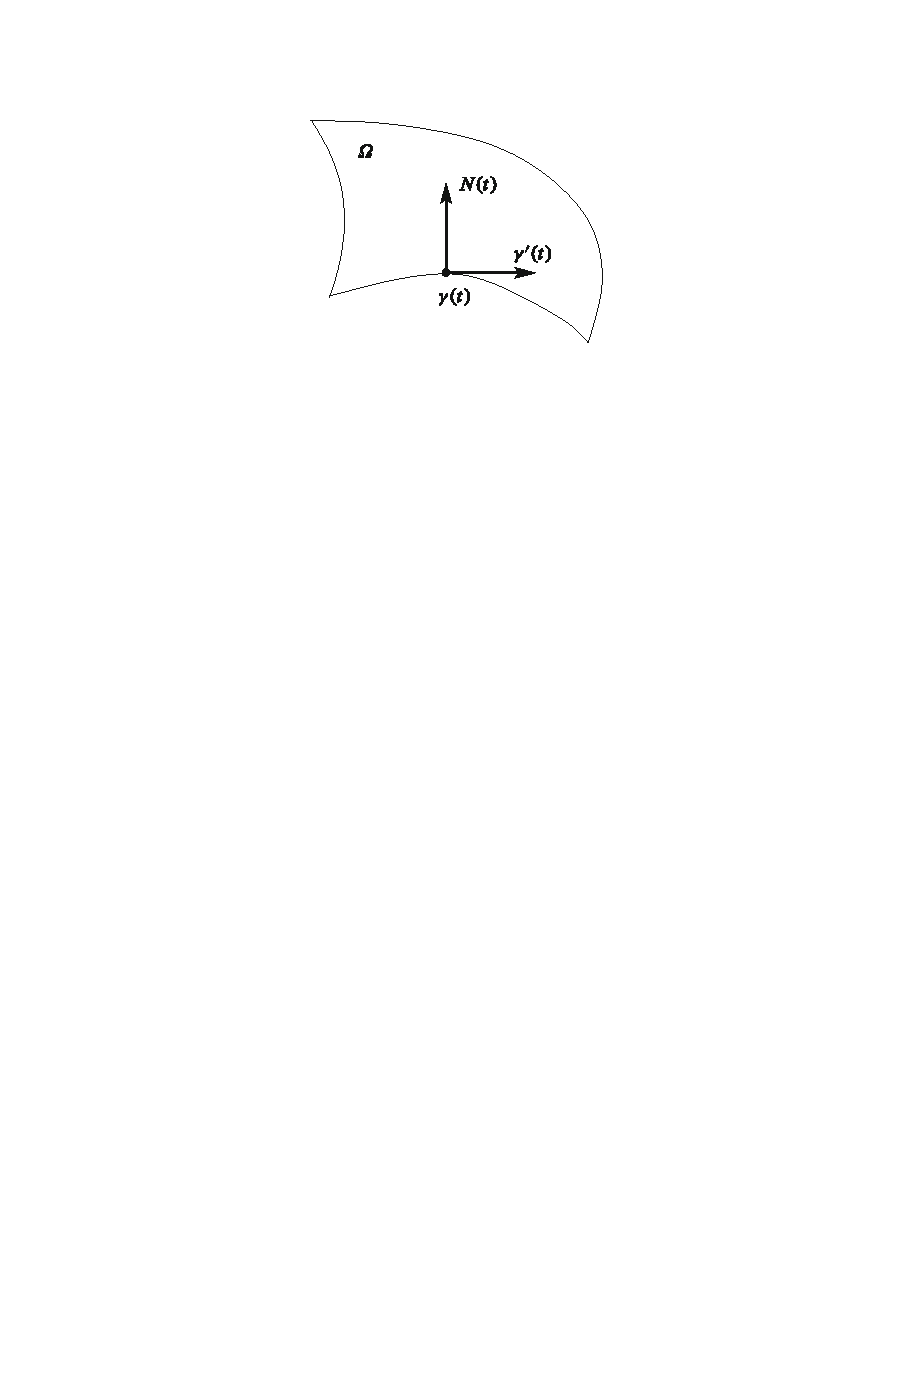
\includegraphics{pictures/inward-normal.pdf}
\caption{$N(t)$ is the inward-pointing normal.}
\end{figure}

From this point onward, we assume for convenience that our curved polygon $\gamma$ is given a unit-speed parametrization, so the unit tangent vector field $T(t)$ is equal 
to $\gamma'(t)$. There is a unique unit normal vector field $N$ along the smooth portions of $\gamma$ such that $(\gamma'(t),N(t))$ is an oriented orthonormal basis for 
$T_{\gamma(t)}M$ for each $t$. If $\gamma$ is positively oriented as the boundary of $\Omega$, this is equivalent to $N$ being the inward-pointing normal to $\partial N$. 
We define the signed curvature of $\gamma$ at smooth points of $\gamma$ by
\[\kappa_N=\langle D_t\gamma'(t),N(t)\rangle_g.\]
By differentiating $|\gamma'(t)|_g\equiv 1$, we see that $D_t\gamma'(t)$ is orthogonal to $\gamma'(t)$, and therefore we can write $D_t\gamma'(t)=\kappa_NN(t)$, and the 
(unsigned) geodesic curvature of $\gamma$ is $\kappa(t)=|\kappa_N(t)|$. The sign of $N(t)$ is positive if $\gamma$ is curving toward $\Omega$, and negative if it is 
curving away.
\begin{theorem}[\textbf{The Gauss-Bonnet Formula}]
Let $(M,g)$ be an oriented Riemannian $2$-manifold. Suppose $\gamma$ is a positively oriented curved polygon in $M$, and $\Omega$ is its interior. Then
\begin{align}\label{Guass Bonnet formula-1}
\int_{\Omega}KdA+\int_{\gamma}\kappa_Nds+\sum_{i=1}^{k}\eps_i=2\pi.
\end{align}
where $K$ is the Gaussian curvature of $g$, $dA$ is its Riemannian volume form, $\eps_1,\dots,\eps_k$ are the exterior angles of $\gamma$.
\end{theorem}
\begin{proof}
Let $(a_0,\dots,a_k)$ be an admissible partition of $[a,b]$, and let $(x,y)$ be oriented smooth coordinates on an open set $U$ containing $\widebar{\Omega}$. Let $\theta:[a,b]\to\R$ 
be a tangent angle function for $\gamma$. Using the rotation index theorem and the fundamental theorem of calculus, we can write
\begin{align}\label{Guass Bonnet formula-2}
2\pi=\theta(b)-\theta(a)=\sum_{i=1}^{k}\eps_i+\sum_{i=1}^{k}\int_{a_{i-1}}^{a_i}\theta'(t)dt.
\end{align}
To prove $(\ref{Guass Bonnet formula-1})$, we need to derive a relationship among $\theta'$, $\kappa_N$ and $K$. Let $(E_1,E_2)$ be the oriented $g$-orthonormal frame 
obtained by applying the Gram-Schmidt algorithm to $(\partial_x,\partial_y)$ as before. Then by definition of $\theta$ and $N$, the following formulas hold at smooth 
points of $\gamma$:
\[\gamma'(t)=\cos\theta(t)E_1|_{\gamma(t)}+\sin\theta(t)E_2|_{\gamma(t)},\quad N(t)=-\sin\theta(t)E_1|_{\gamma(t)}+\cos\theta(t)E_2|_{\gamma(t)}.\]
Differentiating $\gamma'$ (and omitting the $t$ dependence from the notation for simplicity), we get
\begin{align*}
D_t\gamma'&=-(\sin\theta)\theta'E_1+(\cos\theta)\nabla_{\gamma'}E_1+(\cos\theta)\theta'E_2+(\sin\theta)\nabla_{\gamma'}E_2\\
&=\theta'N+(\cos\theta)\nabla_{\gamma'}E_1+(\sin\theta)\nabla_{\gamma'}E_2.
\end{align*}
Next we analyze the covariant derivatives of $E_1$ and $E_2$. Let $\omega=\omega_2^1$ be the connection one form, that is, 
\[\nabla_vE_2=\omega(v)E_1,\quad\nabla_vE_1=-\omega(v)E_2.\] 
Using this, we can compute
\begin{align*}
\kappa_N&=\langle D_t\gamma',N\rangle\\
&=\langle\theta'N,N\rangle+\cos\theta\langle\nabla_{\gamma'}E_1,N\rangle+\sin\theta\langle\nabla_{\gamma'}E_2,N\rangle\\
&=\theta'-\cos\theta\langle\omega(\gamma')E_2,N\rangle+\sin\theta\langle\omega(\gamma')E_1,N\rangle\\
&=\theta'-\cos^2\theta\omega(\gamma')-\sin^2\theta\omega(\gamma')\\
&=\theta'-\omega(\gamma').
\end{align*}
Therefore, $(\ref{Guass Bonnet formula-2})$ becomes
\begin{align*}
2\pi&=\sum_{i=1}^{k}\eps_i+\sum_{i=1}^{k}\int_{a_{i-1}}^{a_i}\kappa_N(t)dt+\sum_{i=1}^{k}\int_{a_{i-1}}^{a_i}\omega(\gamma'(t))dt\\
&=\sum_{i=1}^{k}\eps_i+\int_{\gamma}\kappa_Nds+\int_{\gamma}\omega.
\end{align*}
The theorem will therefore be proved if we can show that
\begin{align}\label{Guass Bonnet formula-3}
\int_{\gamma}\omega=\int_{\Omega}KdA.
\end{align}
Because $\Omega$ is a smooth manifold with corners, we can apply Stokes's theorem and conclude that the left-hand side of $(\ref{Guass Bonnet formula-3})$ is equal to 
$\int_{\Omega}d\omega$. The last step of the proof is to show that $d\omega=KdA$. This follows from the general formula relating the curvature tensor and the connection 
$1$-forms given in Proposition~\ref{Riemann Levi-Civita sturcture equation}:
\[\Omega_2^1=d\omega_2^1=d\omega.\]
and therefore
\[KdA(E_1,E_2)=K=\langle R(E_1,E_2)E_2,E_1\rangle=\langle\Omega_2^1(E_1,E_2)E_1,E_1\rangle=\Omega_2^1(E_1,E_2)=d\omega(E_1,E_2).\]
This completes the proof.
\end{proof}
The following local-to-global theorems of plane geometry follow immediately from the Gauss-Bonnet formula.
\begin{corollary}[\textbf{Angle-Sum Theorem}]\label{Riemann triangle interior sum}
Let $(M,g)$ be an oriented Riemannian $2$-manifold. Suppose $\gamma$ is a positively oriented curved triangle in $M$, and $\Omega$ is its interior. Then
\begin{align}\label{Riemann triangle interior sum-1}
\sum_{i=1}^{3}\theta_i=\pi+\int_{\Omega}KdA+\int_{\gamma}\kappa_Nds.
\end{align}
where $K$ is the Gaussian curvature of $g$ and $\theta_1,\theta_2,\theta_3$ are the interior angles of $\gamma$.
\end{corollary}
\begin{corollary}[\textbf{Total Curvature Theorem}]
If $\gamma:[a,b]\to\R^2$ is a smooth, unitspeed, simple closed curve such that $\gamma'(a)=\gamma'(b)$, and $N$ is the inward-pointing normal, then
\[\int_a^b\kappa_Nds=2\pi.\]
\end{corollary}
\subsection{The Gauss-Bonnet theorem}
Let $M$ be a smooth, compact $2$-manifold. A \textbf{curved triangle in $\bm{M}$} is a curved polygon with exactly three edges and three vertices. A 
\textbf{smooth triangulation of $\bm{M}$} is a finite collection of curved triangles with disjoint interiors such that the union of the triangles with their interiors is 
$M$, and the intersection of any pair of triangles (if not empty) is either a single vertex of each or a single edge of each. Every smooth, compact surface possesses a 
smooth triangulation. In fact, it was proved by Tibor Rad\'o in $1925$ that every compact topological $2$-manifold possesses a triangulation (without the assumption of 
smoothness of the edges, of course), in which every edge belongs to exactly two triangles. There is a proof for the smooth case that is not terribly hard, based on 
choosing geodesic triangles contained in convex geodesic balls.\par
If $M$ is a triangulated $2$-manifold, the Euler characteristic of $M$ (with respect to the given triangulation) is defined to be 
\[\chi(M)=V-E+F,\]
where $V$ is the number of vertices in the triangulation, $E$ is the number of edges, and $F$ is the number of faces (the interiors of the triangles). It is an important 
result of algebraic topology that the Euler characteristic is in fact a topological invariant, and is independent of the choice of triangulation.
\begin{theorem}[\textbf{The Gauss-Bonnet Theorem}]
If $(M,g)$ is a smoothly triangulated compact Riemannian $2$-manifold, then
\[\int_MKdA=2\pi\chi(M).\]
\end{theorem}
\begin{proof}
We may as well assume that $M$ is connected, because if not we can prove the theorem for each connected component and add up the results.\par
First consider the case in which $M$ is orientable. In this case, we can choose an orientation for $M$, and then $\int_MKdA$ gives the same result whether we interpret 
$dA$ as the Riemannian density or as the Riemannian volume form, so we will use the latter interpretation for the proof. Let $\{\Omega_i:i=1,\dots,F\}$ denote the faces 
of the triangulation, and for each $i$, let $\{\gamma_{ij}:j=1,2,3\}$ be the edges of $\Omega_i$ and $\{\theta_{ij}:j=1,2,3\}$ its interior angles. Since each exterior 
angle is $\pi$ minus the corresponding interior angle, applying the Gauss-Bonnet formula to each triangle and summing over $i$ gives
\begin{align}\label{surface Guass-Bonnet-1}
\sum_{i=1}^{F}\sum_{j=1}^{3}\theta_{ij}=\pi F+\sum_{i=1}^{F}\int_{\Omega_i}KdA+\sum_{i=1}^{F}\sum_{j=1}^{3}\int_{\gamma_{ij}}\kappa_Nds.
\end{align}
Note that each edge integral appears exactly twice in the above sum, with opposite orientations, so the integrals of $\kappa_N$ all cancel out. Thus $(\ref{surface Guass-Bonnet-1})$ 
becomes
\begin{align}\label{surface Guass-Bonnet-2}
\sum_{i=1}^{F}\sum_{j=1}^{3}\theta_{ij}=\pi F+\int_{M}KdA.
\end{align}
Note also that each interior angle $\theta_{ij}$ appears exactly once. At each vertex, the angles that touch that vertex must have interior measures that add up to $2\pi$; 
thus the angle sum can be rearranged to give exactly $2\pi V$. Equation $(\ref{surface Guass-Bonnet-2})$ thus can be written
\begin{align}\label{surface Guass-Bonnet-3}
2\pi V=\pi F+\int_{M}KdA.
\end{align}
Finally, since each edge appears in exactly two triangles, and each triangle has exactly three edges, the total number of edges counted with multiplicity is $2E=3F$, where 
we count each edge once for each triangle in which it appears. This means that $F=2E-2F$, so $(\ref{surface Guass-Bonnet-3})$ finally becomes
\begin{align*}
\int_MKdA=2\pi V-\pi F=2\pi V-2\pi E+2\pi F=2\pi\chi(M).
\end{align*}
Now suppose $M$ is nonorientable. Then there is an orientable connected smooth manifold $\widehat{M}$ that admits a $2$-sheeted smooth covering $\hat{\pi}:\widehat{M}\to M$, and then $\widehat{M}$ is compact since $M$ is. If we endow $\widehat{M}$ with the metric $\hat{g}=\hat{\pi}^*g$, then the Riemannian density of $\hat{g}$ is given by $\widehat{dA}=\hat{\pi}^*dA$, and its Gaussian curvature is $\hat{K}=\hat{\pi}^*K$, so $\hat{\pi}^*(KdA)=\hat{K}\widehat{dA}$ and we get
\[\int_{\widehat{M}}\hat{K}\widehat{dA}=2\int_MKdA.\]

To compare the Euler characteristics, we will show that the given triangulation of $M$ "lifts" to a smooth triangulation of $\widehat{M}$. To see this, let $\gamma$ be any curved triangle in $M$ and let $\Omega$ be its interior. By definition, this means that there exists a smooth chart $(U,\varphi)$ whose domain contains $\widebar{\Omega}$ and whose image is a disk $D\sub\R^2$, and such that $\varphi(\widebar{\Omega})=\widebar{\Omega}_0$, where $\Omega_0$ is the interior of a curved triangle $\gamma_0$ in $\R^2$. Then $\varphi^{-1}$ is an embedding of $D$ into $M$, which restricts to a diffeomorphism $F:\widebar{\Omega}_0\to\widebar{\Omega}$. Because $D$ is simply connected, it follows that $\varphi^{-1}$ (and therefore also $F$) has a lift to $\widehat{M}$, which is smooth because $\widehat{\pi}$ is a local diffeomorphism; and because the covering is two-sheeted, there are exactly two such lifts $F_1,F_2$. Each lift is injective because $\widebar{\pi}\circ F_i=F$, which is injective, and their images are disjoint because if two lifts agree at a point, they must be identical. From this it is straightforward to verify that the lifted curved triangles form a triangulation of $\widehat{M}$ with twice as many vertices, edges, and faces as that of $M$, and thus $\chi(\widehat{M})=2\chi(M)$. Substituting these relations into the Gauss-Bonnet theorem for $\widehat{M}$ and dividing through by $2$, we obtain the relation for $M$.
\end{proof}
The significance of this theorem cannot be overstated. Together with the classification theorem for compact surfaces, it gives us very detailed information about the possible Gaussian curvatures for metrics on compact surfaces. The classification theorem says that every compact, connected, orientable $2$-manifold $M$ is homeomorphic to a sphere or a connected sum of $n$ tori, and every nonorientable one is homeomorphic to a connected sum of $n$ copies of the real projective plane $\RP^2$; the number $n$ is called the genus of $M$. (The sphere is said to have genus zero.) By constructing simple triangulations, one can show that the Euler characteristic of an orientable surface of genus $n$ is $2-2n$, and that of a nonorientable one is $2-n$. The following corollary follows immediately from the Gauss-Bonnet theorem.
\begin{corollary}\label{Riemann surface topology to curvature}
Let $(M,g)$ be a compact Riemannian $2$-manifold and let $K$ be its Gaussian curvature.
\begin{itemize}
\item[(a)] If $M$ is homeomorphic to the sphere or the projective plane, then $K>0$ somewhere.
\item[(b)] If $M$ is homeomorphic to the torus or the Klein bottle, then either $K\equiv 0$ or $K$ takes on both positive and negative values.
\item[(c)] If $M$ is any other compact surface, then $K<0$ somewhere.
\end{itemize}
\end{corollary}
\begin{proof}
Note that $\chi(S^2)=2$, $\chi(\RP^2)=1$, $\chi(T^2)=0$, and other surfaces possess negative Euler characteristics.
\end{proof}
In Corollary\ref{Riemann surface topology to curvature} we assumed we knew the topology of $M$ and drew conclusions about the possible curvatures it could support. In the following corollary we reverse our 
point of view, and use assumptions about the curvature to draw conclusions about the topology of the manifold.
\begin{corollary}\label{Riemann surface curvature to topology}
Let $(M,g)$ be a compact Riemannian $2$-manifold and $K$ its Gaussian curvature.
\begin{itemize}
\item[(a)] If $K>0$ everywhere on $M$, then the universal covering manifold of $M$ is homeomorphic to $S^2$, and $\pi_1(M)$ is either trivial or isomorphic to the two element group $\Z/2\Z$.
\item[(b)] If $K\leq 0$ everywhere on $M$, then the universal covering manifold of $M$ is homeomorphic to $\R^2$, and $\pi_1(M)$ is infinite.
\end{itemize}
\end{corollary}
\begin{proof}
Suppose first that $M$ has positive Gaussian curvature. From the Gauss-Bonnet theorem, $M$ has positive Euler characteristic. The classification theorem for compact surfaces shows that the only such surfaces are the sphere (with trivial fundamental group) and the projective plane (with fundamental group isomorphic to $\Z/2\Z$), both of which are covered by the sphere.\par
On the other hand, suppose $M$ has nonpositive Gaussian curvature. Then its Euler characteristic is nonpositive, so it is either an orientable surface of genus $n\geq 1$ or a nonorientable one of genus $n\geq 2$. Thus the universal covering space of $M$ is $\R^2$ if $M$ is the torus or the Klein bottle, and $\B^2$ in all other cases, both of which are homeomorphic to $\R^2$. The fact that the universal covering space is noncompact implies that the universal covering map has infinitely many sheets, and therefore $\pi_1(M)$ is infinite.
\end{proof}
\section{Jacobi fields}
Our goal for the remainder of this chapter is to generalize to higher dimensions some of the geometric and topological consequences of the Gauss-Bonnet theorem. We need to develop a new approach: instead of using Stokes's theorem and differential forms to relate the curvature to global topology as in the proof of the Gauss-Bonnet theorem, we study the way that curvature affects the behavior of nearby geodesics. Roughly speaking, positive curvature causes nearby geodesics to converge, while negative curvature causes them to spread out. In order to draw topological consequences from this fact, we need a quantitative way to measure the effect of curvature on a one-parameter family of geodesics.\par
We begin by deriving the Jacobi equation, which is an ordinary differential equation satisfied by the variation field of any one-parameter family of geodesics. A vector field satisfying this equation along a geodesic is called a \textbf{Jacobi field}. We then introduce conjugate points, which are pairs of points along a geodesic where some nontrivial Jacobi field vanishes. Intuitively, if $p$ and $q$ are conjugate along a geodesic, one expects to find a one-parameter family of geodesic segments that start at $p$ and end (almost) at $q$.\par
After defining conjugate points, we prove a simple but essential fact: the points conjugate to p are exactly the points where $\exp_p$ fails to be a local diffeomorphism. We then derive an expression for the second derivative of the length functional with respect to proper variations of a geodesic, called the second variation formula. Using this formula, we prove another essential fact about conjugate points: once a geodesic passes its first conjugate point, it is no longer minimizing. The converse of this statement, however, is untrue: a geodesic can cease to be minimizing before it reaches its first conjugate point. Finally, we study the set of points where geodesics starting at a given point $p$ cease to minimize, called the cut locus of $p$.
\subsection{The Jacobi equation}
Let $(M,g)$ be an $n$-dimensional (pseudo-)Riemannian manifold. In order to study the effect of curvature on nearby geodesics, we focus on variations through geodesics. Suppose, therefore, that $I,K\sub\R$ are intervals, $\gamma:I\to M$ is a geodesic, and $\Gamma:K\times I\to M$ is a variation of $\gamma$. We say that $\Gamma$ is a variation through geodesics if each of the main curves $\Gamma_s(t)=\Gamma(s,t)$ is also a geodesic. (In particular, this requires that $\Gamma$ be smooth.) Our first goal is to derive an equation that must be satisfied by the variation field of a variation through geodesics.
\begin{theorem}[\textbf{The Jacobi Equation}]\label{Jacobi equation}
Let $(M,g)$ be a (pseudo-)Riemannian manifold, let $\gamma$ be a geodesic in $M$, and let $J$ be a vector field along $\gamma$. If $J$ is the variation field of a variation through geodesics, then $J$ satisfies the following equation, called the \textbf{Jacobi equation}:
\begin{align}\label{Jacobi equation-1}
D_t^2J+R(J,\gamma')\gamma'=0.
\end{align}
\end{theorem}
\begin{proof}
The geodesic equation tells us that $D_t\partial_t\Gamma\equiv 0$ for all $(s,t)$. We can take the covariant derivative of this equation with respect to $s$, yielding $D_sD_t\partial_t\Gamma\equiv 0$. Using Proposition~\ref{Riemann curvature second derivatire curve} to commute the covariant derivatives along $\gamma$, we compute
\begin{align*}
0=D_sD_t\partial_t\Gamma=D_tD_s\partial_t\Gamma+R(\partial_s\Gamma,\partial_t\Gamma)\partial_t\Gamma=D_tD_t\partial_s\Gamma+R(\partial_s\Gamma,\partial_t\Gamma)\partial_t\Gamma
\end{align*}
where the last step follows from the symmetry lemma. Evaluating at $s=0$, where $\partial_s\Gamma(0,t)=J(t)$ and $\partial_t\Gamma(0,t)=\gamma'(t)$, we get $(\ref{Jacobi equation})$.
\end{proof}
A smooth vector field along a geodesic that satisfies the Jacobi equation is called a \textbf{Jacobi field}. As the following proposition shows, the Jacobi equation  can be written as a system of second-order linear ordinary differential equations, so it has a unique solution given initial values for $J$ and $D_tJ$ at one point.
\begin{proposition}\label{Riemann Jacobi field unique}
Let $(M,g)$ be a (pseudo-)Riemannian manifold. Suppose $I\sub\R$ is an interval, $\gamma:I\to\R$ is a geodesic, $a\in I$, and $p=\gamma(a)$. For every pair of vectors $v,w\in T_pM$, there is a unique Jacobi field $J$ along $\gamma$ satisfying the initial conditions
\[J(a)=v,\quad D_tJ(a)=w.\]
\end{proposition}
\begin{proof}
Choose a parallel orthonormal frame $(E_i)$ along $\gamma$, and write $v=v^iE_i(a)$, $w=w^iE_i(a)$, and $\gamma'(t)=y^i(t)E_i(t)$ in terms of this frame. Writing an unknown vector field $J\in\X(\gamma)$ as $J(t)=J^i(t)E_i(t)$, we can express the Jacobi equation as
\[\ddot{J}^l(t)+R_{ijk}^l(\gamma(t))J^i(t)y^j(t)y^k(t)=0.\]
This is a system of $n$ linear second-order ODEs for the $n$ functions $J^i:I\to\R$. Making the substitution $W^i=\dot{J}^i$ converts it to the following equivalent first-order linear system for the $2n$ unknown functions $(J^i,W^i)$:
\begin{align*}
\dot{J}^i(t)&=W^i(t),\\
\dot{W}^i(t)&=-R_{ijk}^l(\gamma(t))J^i(t)y^j(t)y^k(t).
\end{align*}
Then Theorem~\ref{linear ODE existence unique} guarantees the existence and uniqueness of a smooth solution on the whole interval $I$ with arbitrary initial conditions $J^i(a)=v^i$, $W^i(a)=w^i$. Since $D_tJ(a)=\dot{J}^i(a)E_i(a)=W^i(a)E_i(a)=w$, it follows that $J(t)=J^i(t)E_i(t)$ is the desired Jacobi field.
\end{proof}
Given a geodesic $\gamma$, let $\J(\gamma)\sub\X(\gamma)$ denote the set of Jacobi fields along $\gamma$.
\begin{corollary}\label{Riemann Jacobi field dim}
Suppose $(M,g)$ is a (pseudo-)Riemannian manifold of dimension $n$, and $\gamma$ is any geodesic in $M$. Then $\J(\gamma)$ is a $2n$-dimensional linear subspace of $\X(\gamma)$.
\end{corollary}
\begin{proof}
Because the Jacobi equation is linear, $\J(\gamma)$ is a linear subspace of $\X(\gamma)$. Let $p=\gamma(a)$ be any point on $\gamma$, and consider the linear map from $J(\gamma)$ to $T_pM\times T_pM$ by sending $J$ to $(J(a),D_tJ(a))$. The preceding proposition says precisely that this map is bijective.
\end{proof}
The following proposition is a converse to Theorem~\ref{Jacobi equation}; it shows that each Jacobi field along a geodesic segment tells us how some family of geodesics behaves, at least to first order along $\gamma$.
\begin{proposition}\label{Riemann Jacobi field variation}
Let $(M,g)$ be a (pseudo-)Riemannian manifold, and let $\gamma:I\to M$ be a geodesic. If $M$ is complete or $I$ is a compact interval, then every Jacobi 
field along $\gamma$ is the variation field of a variation of $\gamma$ through geodesics.
\end{proposition}
\begin{proof}
Let $J$ be a Jacobi field along $\gamma$. After applying a translation in $t$ (which does not affect either the fact that $\gamma$ is a geodesic or the fact that $J$ is a Jacobi field), we can assume that the interval $I$ contains $0$, and write $p=\gamma(0)$ and $v=\gamma'(0)$. Note that this implies $\gamma(t)=\exp_p(tv)$ for all $t\in I$.\par
Choose a smooth curve $\sigma:(-\eps,\eps)\to M$ and a smooth vector field $V$ along $\sigma$ satisfying
\begin{alignat*}{2}
\sigma(0)&=p     &\quad V(0)&=v\\
\sigma'(0)&=J(0) &\quad D_sV(0)&=D_tJ(0)
\end{alignat*}
where $D_s$ and $D_t$ denote covariant differentiation along $\sigma$ and $\gamma$, respectively. (They are easily constructed in local coordinates around $p$.) We wish to define a variation of $\gamma$ by setting
\begin{align}\label{Riemann Jacobi field variation-1}
\Gamma(s,t)=\exp_{\sigma(s)}(tV(s)).
\end{align}
If $M$ is geodesically complete, this is defined for all $(s,t)\in(-\eps,\eps)\times I$. On the other hand, if $I$ is compact, the fact that the domain of the exponential 
map is an open subset of $TM$ that contains the compact set $\{(p,tv):t\in I\}$ guarantees that there is some $\delta>0$ such that $\Gamma(s,t)$ is defined for all 
$(s,t)\in(-\delta,\delta)\times I$. (This is the tube lemma.)\par
Note that
\begin{align}
\Gamma(0,t)&=\exp_{\sigma(0)}(tV(0))=\exp_p(tv)=\gamma(t), \label{Riemann Jacobi field variation-2}\\
\Gamma(s,0)&=\exp_{\sigma(s)}(0)=\sigma(s).\label{Riemann Jacobi field variation-3}
\end{align}
In particular, $(\ref{Riemann Jacobi field variation-2})$ shows that $\Gamma$ is a variation of $\gamma$. The properties of the exponential map guarantee that $\Gamma$ 
is a variation through geodesics, and therefore its variation field $W(t)=\partial_s\Gamma(0,t)$ is a Jacobi field along $\gamma$.\par
Now, $(\ref{Riemann Jacobi field variation-3})$ implies
\[W(0)=\frac{\partial}{\partial s}\Big|_{s=0}\Gamma(s,0)=\sigma'(0)=J(0).\]
If we can show that $D_tW(0)=D_tJ(0)$ as well, it then follows from the uniqueness of Jacobi fields that $W\equiv J$, and the proposition is proved.\par
Formula $(\ref{Riemann Jacobi field variation-1})$ shows that each main curve $\Gamma_s(t)$ is a geodesic whose initial velocity is $V(s)$, so
\[\partial_t\Gamma(s,0)=\frac{\partial}{\partial t}\Big|_{t=0}\Gamma_s(t)=V(s).\]
It follows from the symmetry lemma that $D_t\partial_s\Gamma=D_s\partial_t\Gamma$, and our choice of $V$ gives
\[D_tW(0)=D_t\partial_s\Gamma(0,0)=D_s\partial_t\Gamma(0,0)=D_sV(0)=D_tJ(0).\]
This finishes the proof.
\end{proof}
\begin{proposition}[\textbf{Local Isometry Invariance of Jacobi Fields}]
Suppose $(M,g)$ and $(\widetilde{M},\tilde{g})$ are (pseudo-)Riemannian manifolds and $\varphi:M\to\widetilde{M}$ is a local isometry. Let $\gamma:I\to M$ 
and $\tilde{\gamma}:I\to\widetilde{M}$ be geodesics related by $\tilde{\gamma}=\varphi\circ\gamma$, and let $J\in\X(\gamma)$, $\widetilde{J}\in\X(\tilde{\gamma})$ 
be related by $d\varphi_{\gamma(t)}(J(t))=\widetilde{J}(t)$ for all $t\in I$. Then $J$ is a Jacobi field if and only if $\widetilde{J}$ is.
\end{proposition}
\begin{proof}
The curvature tensor and covariant derivatire are preserved by a local isometry, therefore the Jacobi equation is also preserved.
\end{proof}
\subsection{Basic computations with Jacobi fields}
There are various situations in which Jacobi fields can be computed explicitly. We begin by describing the most important of these.
\subsubsection{Tangential and normal Jacobi fields}
Along every geodesic $\gamma:I\to M$, there are always two Jacobi fields that we can write down immediately. Because $D_t\gamma'\equiv 0$ and 
$R(\gamma',\gamma')\gamma'\equiv 0$ by antisymmetry of $R$, the vector fields $J_0(t)=\gamma'(t)$ and $J_1(t)=t\gamma'(t)$ both satisfy the Jacobi equation by direct 
computation. If $I$ is compact or $M$ is complete, the vector field $J_0$ is the variation field of the variation $\Gamma(s,t)=\Gamma(s+t)$, while $J_1$ is the 
variation field of $\Gamma(s,t)=\gamma((1+s)t)$. Therefore, these two Jacobi fields just reflect the possible reparametrizations of $\gamma$, and do not tell us 
anything about the behavior of geodesics other than $\gamma$ itself.\par
To distinguish these trivial cases from more informative ones, we make the following definitions. Given a regular curve $\gamma:I\to M$, for each $t\in I$ we let 
$T_{\gamma(t)}^{\top}M\sub T_{\gamma(t)}M$ denote the one-dimensional subspace spanned by $\gamma'(t)$, and $T_{\gamma(t)}^{\bot}M$ its orthogonal complement. A 
\textbf{tangential vector field along $\bm{\gamma}$} is a vector field $V\in\X(\gamma)$ such that $V(t)\in T_{\gamma(t)}^{\top}M$ for all $t$, and a 
\textbf{normal vector field along $\bm{\gamma}$} is one such that $V(t)\in T_{\gamma(t)}^{\bot}M$ for all $t$. Thus a \textbf{normal Jacobi field along $\bm{\gamma}$} 
is a Jacobi field $J$ satisfying $J(t)\bot\gamma'(t)$ for all $t$. Let $\X^{\top}(\gamma)$ and $X^{\bot}(\gamma)$ denote the spaces of smooth normal and tangential 
vector fields along $\gamma$, respectively. When $\gamma$ is a geodesic, $\J^{\top}(\gamma)$ and $\J^{\bot}(\gamma)$ denote the spaces of normal and tangential Jacobi 
fields along $\gamma$, respectively.
\begin{proposition}\label{Riemann normal Jacobi field iff}
Let $(M,g)$ be a (pseudo-)Riemannian manifold. Suppose $\gamma:I\to M$ is a geodesic and $J$ is a Jacobi field along $\gamma$. Then the following are 
equivalent:
\begin{itemize}
\item[(a)] $J$ is a normal Jacobi field.
\item[(b)] $J$ is orthogonal to $\gamma'$ at two distinct points.
\item[(c)] Both $J$ and $D_tJ$ are orthogonal to $\gamma'$ at one point.
\item[(d)] Both $J$ and $D_tJ$ are orthogonal to $\gamma'$ everywhere along $\gamma$.
\end{itemize}
\end{proposition}
\begin{proof}
Define a function $f:I\to\R$ by $f(t)=\langle J(t),\gamma'(t)\rangle$, so that $f(t)\equiv 0$ if and only if $J(t)\bot\gamma'(t)$. Using compatibility with the metric 
and the fact that $D_t\gamma'(t)\equiv 0$, we compute
\begin{align*}
f''(t)&=\langle D_t^2J,\gamma'\rangle=-\langle R(J,\gamma')\gamma',\gamma'\rangle=-R(J,\gamma',\gamma',\gamma')=0
\end{align*}
by the symmetries of the curvature tensor. Thus, by elementary calculus, $f$ is an affine function of $t$.\par
Note that $f'(t)=\langle D_tJ(t),\gamma'(t)\rangle$, which vanishes at $t$ if and only if $D_tJ(t)\bot\gamma'(t)$. It follows that $J(a)$ and $D_tJ(a)$ are orthogonal 
to $\gamma'(a)$ for some $a\in I$ if and only if $f$ and its first derivative vanish at $a$, which happens if and only if $f\equiv 0$. Similarly, $J$ is orthogonal to 
$\gamma'$ at two points if and only if $f$ vanishes at two points, which happens if and only if $f$ is identically zero. If this is the case, then $f'\equiv 0$ as well, 
which implies that both $J$ and $D_tJ$ are orthogonal to $\gamma'$ for all $t$.
\end{proof}
\begin{corollary}\label{Riemann Jaboci tangential normal dim}
Suppose $(M,g)$ is a (pseudo-)Riemannian $n$-manifold and $\gamma:I\to M$ is any nonconstant geodesic. Then $\J^{\bot}(\gamma)$ is a $(2n-2)$-dimensional 
subspace of $\J(\gamma)$, and $J^{\top}(\gamma)$ is a $2$-dimensional subspace. Every Jacobi field can be uniquely decomposed as a sum of a tangential Jacobi field plus 
a normal Jacobi field.
\end{corollary}
\begin{proof}
As we noted in the proof of Corollary~\ref{Riemann Jacobi field dim}, for every $a\in I$, the map from $\J((\gamma)$ to $T_{\gamma(a)}M\oplus T_{\gamma(a)}M$ given by 
$J\mapsto(J(a),D_tJ(a))$ is an isomorphism, and Proposition~\ref{Riemann normal Jacobi field iff} shows that $\J^{\bot}(\gamma)$ is exactly the preimage of the subspace 
consisting of all pairs $(v,w)\in T_{\gamma(a)}M\oplus T_{\gamma(a)}M$ such that $\langle v,\gamma'(a)\rangle=\langle w,\gamma'(a)\rangle=0$. Because this subspace has 
dimension $2n-2$, it follows that $\J^{\bot}(\gamma)$ has the same dimension.\par
On the other hand, $\J^{\top}(\gamma)$ contains $J_0(t)=\gamma'(t)$ and $J_1(t)=t\gamma'(t)$, which are linearly independent over $\R$ because $\gamma'(t)$ never 
vanishes, so it is a subspace of dimension at least $2$. Because $\J^{\top}(\gamma)\cap\J^{\bot}(\gamma)=\{0\}$, the dimension of $\J^{\top}(\gamma)$ must be exactly $2$, 
and we have a direct sum decomposition $\J(\gamma)=\J^{\top}(\gamma)\oplus\J^{\bot}(\gamma)$. This implies that every $J\in\J(\gamma)$ has a unique decomposition $J=J^{\top}+J^{\bot}$, 
with $J^{\top}\in\J^{\top}(\gamma)$ and $J^{\bot}\in\J^{\bot}(\gamma)$.
\end{proof}
\subsubsection{Jacobi fields vanishing at a point}
For many purposes, we will be primarily interested in Jacobi fields that vanish at a particular point. For these, there are some useful explicit formulas.
\begin{figure}[htbp]
\centering
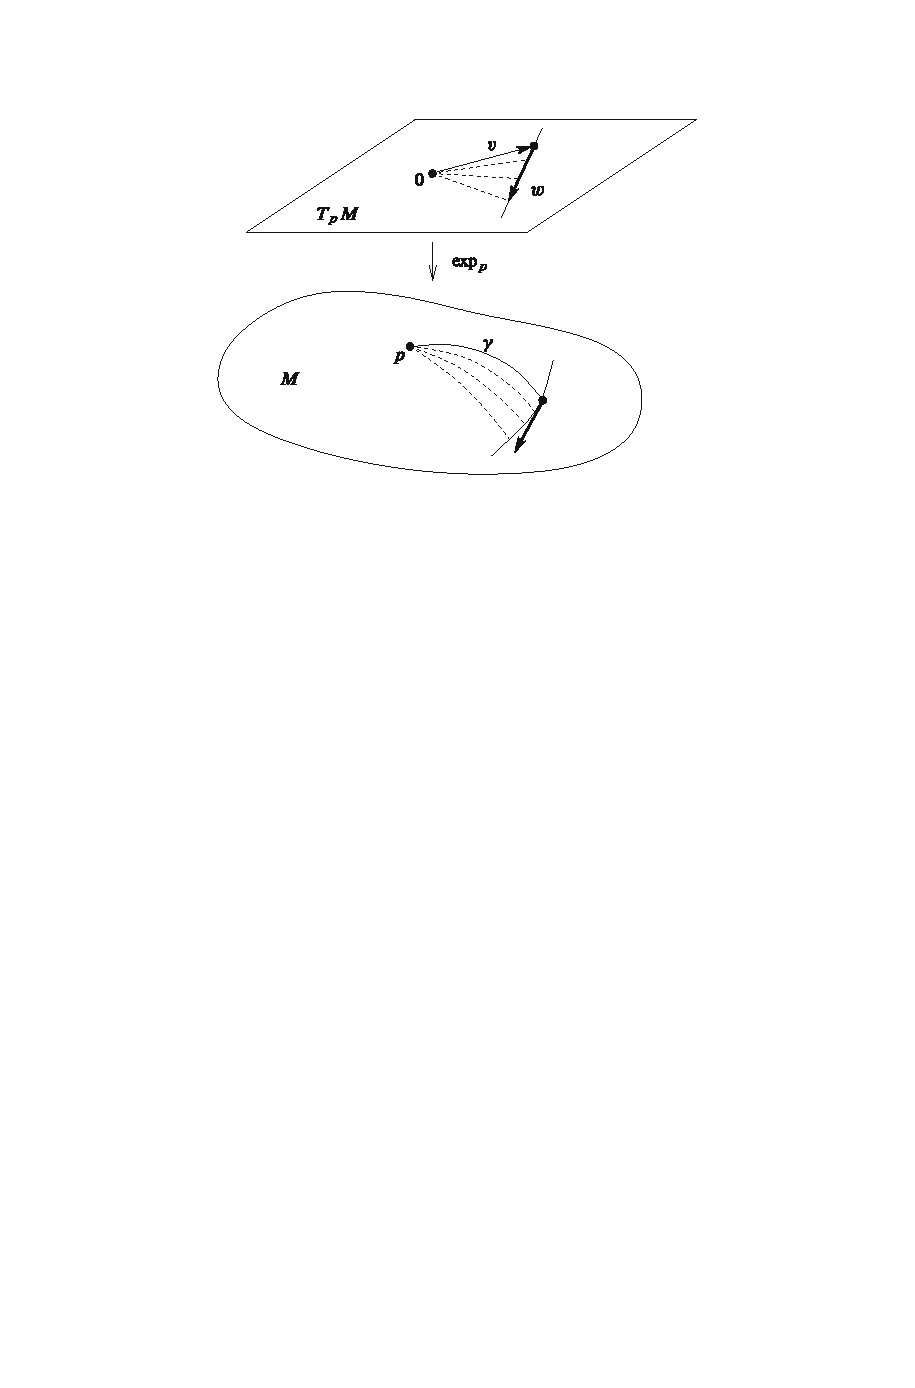
\includegraphics{pictures/Jacobi-field-one-point}
\caption{The variation of Lemma~\ref{Riemann Jacobi vanishing one point lem}.}
\end{figure}
\begin{lemma}\label{Riemann Jacobi vanishing one point lem}
Let $(M,g)$ be a (pseudo-)Riemannian manifold, $I\sub\R$ an interval containing $0$, and $\gamma:I\to M$ a geodesic. Suppose $J:I\to M$ is a Jacobi field 
such that $J(0)=0$. If $M$ is geodesically complete or $I$ is compact, then $J$ is the variation field of the following variation of $\gamma$ through geodesics:
\begin{align}\label{Riemann Jacobi vanishing one point variation field}
\Gamma(s,t)=\exp_p(t(v+sw)).
\end{align}
where $p=\gamma(0)$, $v=\gamma'(0)$, and $w=D_tJ(0)$.
\end{lemma}
\begin{proof}
The proof of Proposition~\ref{Riemann Jacobi field variation} showed that $J$ is the variation field of a variation $\Gamma$ of the form $(\ref{Riemann Jacobi field variation-1})$, 
with $\sigma$ any smooth curve satisfying $\sigma(0)=p$ and $\sigma'(0)=0$, and $V$ a smooth vector field along $\sigma$ with $V(0)=v$ and $D_sV(0)=w$. In this case, we 
can take $\sigma(s)\equiv p$ and $V(s)=v+sw\in T_pM$, yielding $(\ref{Riemann Jacobi vanishing one point variation field})$.
\end{proof}
This result leads to some explicit formulas for all of the Jacobi fields vanishing
at a point.
\begin{proposition}[\textbf{Jacobi Fields Vanishing at a Point}]\label{Riemann Jacobi vanishing one point}
Let $(M,g)$ be a (pseudo-)Riemannian n-manifold and $p\in M$. Suppose $\gamma:I\to M$ is a geodesic such that $0\in I$ and $\gamma'(0)=p$. For every $w\in T_pM$, 
the Jacobi field $J$ along $\gamma$ such that $J(0)=0$ and $D_tJ(0)=w$ is given by
\begin{align}\label{Riemann Jacobi vanishing one point expression}
J(t)=d(\exp_p)_{tv}(tw),
\end{align}
where $v=\gamma'(0)$, and we regard $tw$ as an element of $T_{tv}(T_pM)$ by means of the canonical identification $T_{tv}(T_pM)\cong T_pM$. If $(x^i)$ are normal 
coordinates on a normal neighborhood of $p$ containing the image of $\gamma$, then $J$ is given by the formula
\begin{align}\label{Riemann Jacobi vanishing one point coordinate form}
J(t)=tw^i\partial_i|_{\gamma(t)},
\end{align}
where $w^i\partial_i|_0$ is the coordinate representation of $w$.
\end{proposition}
\begin{figure}[htbp]
\centering
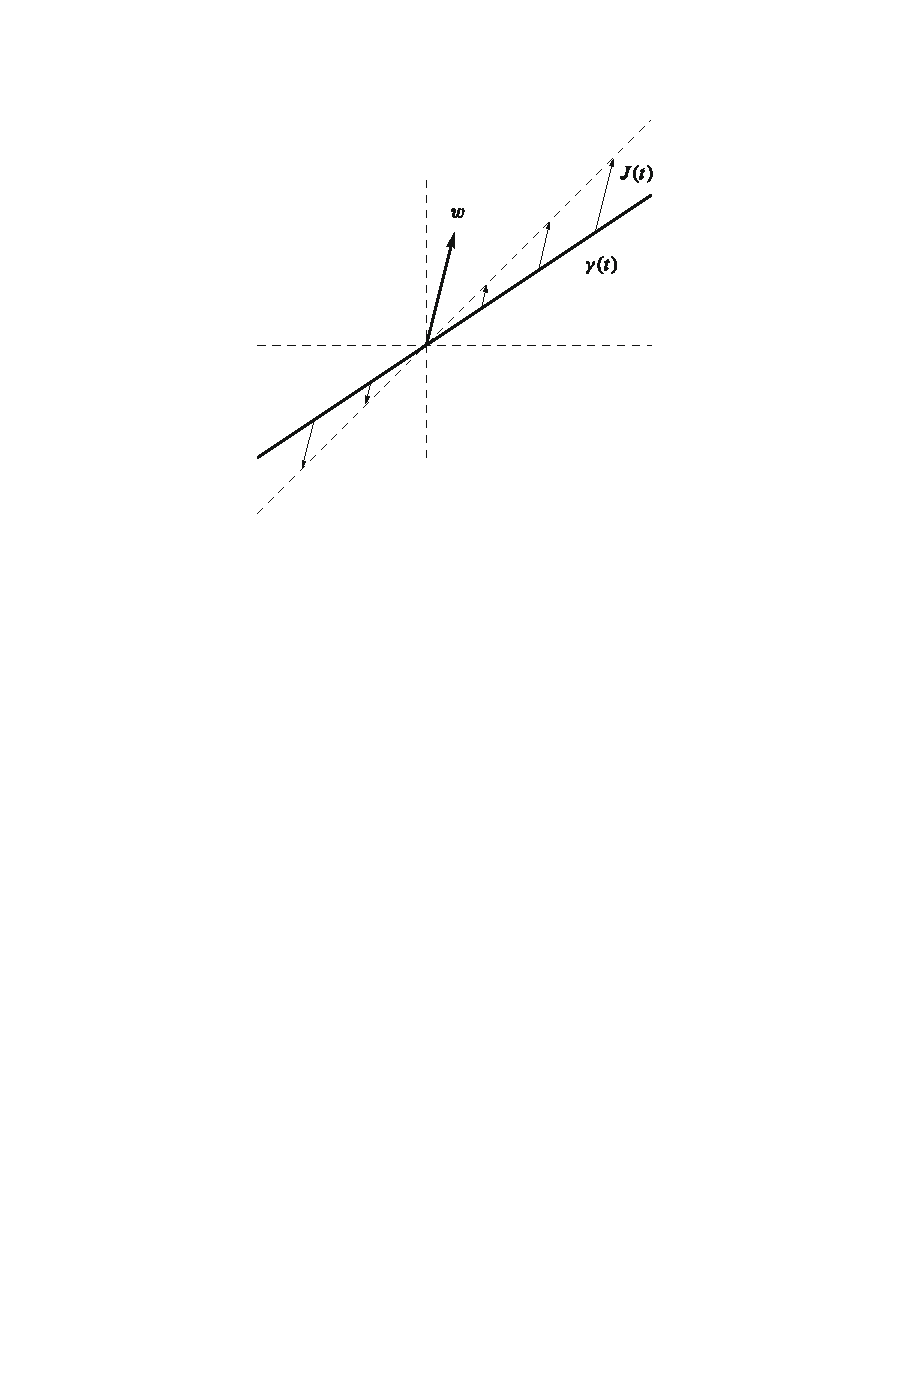
\includegraphics{pictures/Jacobi-field-normal-coordinate}
\caption{A Jacobi field in normal coordinates.}
\end{figure}
\begin{proof}
Under the given hypotheses, Lemma~\ref{Riemann Jacobi vanishing one point lem} showed that the restriction of $J$ to any compact interval containing $0$ is the 
variation field of a variation $\Gamma$ through geodesics of the form $(\ref{Riemann Jacobi vanishing one point variation field})$. Using the chain rule to compute $J(t)=\partial_s\Gamma(0,t)$, 
we arrive at $(\ref{Riemann Jacobi vanishing one point expression})$. Because every $t$ in the domain of $\Gamma$ is contained in some such compact interval, the formula holds for all such $t$.\par
In normal coordinates, the coordinate representation of the exponential map is the identity, so $\Gamma$ can be written explicitly in coordinates as
\[\Gamma(s,t)=(t(v^1+sw^1),\dots,t(v^n+sw^n)).\]
Differentiating $\Gamma(s,t)$ with respect to $s$ and setting $s=0$ shows that its variation field $J$ is given by $(\ref{Riemann Jacobi vanishing one point coordinate form})$.
\end{proof}
\begin{corollary}\label{Riemann value of Jacobi field along radial}
Suppose $(M,g)$ is a (pseudo-)Riemannian manifold and $U$ is a normal neighborhood of $p\in M$. For each $q\in U\setminus\{p\}$, every vector in $T_qM$ is 
the value of a Jacobi field $J$ along a radial geodesic such that $J$ vanishes at $p$.
\end{corollary}
\begin{proof}
Let $(x^i)$ be normal coordinates on $U$. Given $q=(q^1,\dots,q^n)\in U\setminus\{p\}$ and $w=w^iw^i\partial_i|_q\in T_qM$, the curve $\gamma(t)=(tq^1,\dots,tq^n)$ is a 
radial geodesic satisfying $\gamma(0)=p$ and $\gamma(1)=q$. The previous proposition showed that $J(t)=tw^i\partial_i|_{\gamma(t)}$ is a Jacobi field along $\gamma$. 
Because $J(0)=0$ and $J(1)=w$, the result follows.
\end{proof}
\subsubsection{Jacobi fields in constant-curvature spaces}
For metrics with constant sectional curvature, we have a different kind of explicit formula for Jacobi fields---this one expresses a Jacobi field as a scalar multiple 
of a parallel vector field. To handle the various cases concisely, for each $c\in\R$, let us define a function $s_c:\R\to\R$ by
\begin{equation}\label{Riemann Jacobi constant curvature function}
s_c(t)=\begin{cases}
t,&\text{if $c=0$};\\[8pt]
R\sin\dfrac{t}{R},&\text{if $c=\dfrac{1}{R^2}>0$};\\[8pt]
R\sinh\dfrac{t}{R},&\text{if $c=-\dfrac{1}{R^2}<0$}.
\end{cases}
\end{equation}
\begin{proposition}[\textbf{Jacobi Fields in Constant Curvature}]\label{Riemann Jacobi constant curvature}
Suppose $(M,g)$ is a Riemannian manifold with constant sectional curvature $c$, and $\gamma$ is a unit-speed geodesic in $M$. The normal Jacobi fields along $\gamma$ 
vanishing at $t=0$ are the vector fields of the form
\begin{align}\label{Riemann Jacobi constant curvature-1}
J(t)=ks_c(t)E(t),
\end{align}
wher $E$ is any parallel unit normal vector field along $\gamma$, $k$ is an arbitrary constant, and $s_c$ is defined by $(\ref{Riemann Jacobi constant curvature function})$. 
The initial derivative of such a Jacobi field is
\begin{align}\label{Riemann Jacobi constant curvature-2}
D_tJ(0)=kE(0).
\end{align}
and its norm is
\begin{align}\label{Riemann Jacobi constant curvature-3}
|J(t)|=|s_c(t)||D_tJ(0)|.
\end{align}
\end{proposition}
\begin{proof}
Since $g$ has constant curvature, its curvature endomorphism is given by the formula of Proposition~\ref{Riemann constant curvature iff}:
\[R(x,y)v=c(\langle y,v\rangle x-\langle x,v\rangle y).\]
Substituting this into the Jacobi equation, we find that a normal Jacobi field $J$ satisfies
\begin{align}\label{Riemann Jacobi constant curvature-4}
0=D_t^2J+c(\langle \gamma',\gamma'\rangle J-\langle J,\gamma'\rangle \gamma')=D_t^2J+cJ,
\end{align}
where we have used the facts that $|\gamma'|=1$ and $\langle J,\gamma'\rangle=0$.\par
Since $(\ref{Riemann Jacobi constant curvature-4})$ says that the second covariant derivative of $J$ is a multiple of $J$ itself, it is reasonable to try to construct a 
solution by choosing an arbitrary parallel unit normal vector field $E$ along $\gamma$ and setting $J(t)=u(t)E(t)$ for some function $u$ to be determined. Plugging this 
into $(\ref{Riemann Jacobi constant curvature-4})$, we find that $J$ is a Jacobi field if and only if $u$ is a solution to the differential equation
\[u''(t)+cu(t)=0.\]
It is an easy matter to solve this ODE explicitly. In particular, the solutions satisfying $u(0)=0$ are constant multiples of $s_c$. This construction yields all the 
normal Jacobi fields vanishing at $0$, since there is an $(n-1)$-dimensional space of them, and the space of parallel normal vector fields has the same dimension.\par
To prove the last two statements, suppose $J$ is given by $(\ref{Riemann Jacobi constant curvature-1})$, and compute
\[D_tJ(0)=ks_c'(0)E(0)=kE(0).\]
since $s_c'(0)=1$ in every case. Because $E$ is a unit vector field, $|D_tJ(0)|=|k|$ and $(\ref{Riemann Jacobi constant curvature-2})$ follows.
\end{proof}
Here is our first significant application of Jacobi fields. Because every tangent vector in a normal neighborhood is the value of a Jacobi field vanishing at the origin 
by Corollary~\ref{Riemann value of Jacobi field along radial}, Proposition~\ref{Riemann Jacobi constant curvature} yields explicit formulas for constant curvature metrics in 
normal coordinates. To set the stage, we will rewrite the Euclidean metric on $\R^n$ in a form that is somewhat more convenient for these computations.\par
Let $\pi:\R^n\setminus\{0\}\to S^{n-1}$ be the radial projection
\begin{align}\label{Riemann R^n radial projection}
\pi(x)=\frac{x}{|x|},
\end{align}
and define a symmetric $2$-tensor field on $\R^n\setminus\{0\}$ by
\begin{align}\label{Riemann R^n metric new form}
\hat{g}=\pi^*\mathring{g},
\end{align}
where $\mathring{g}$ is the round metric on $S^{n-1}$.
\begin{lemma}
On $\R^n\setminus\{0\}$, the metric $\hat{g}=\pi^*\mathring{g}$ and the Euclidean metric $\widebar{g}$ are related by
\begin{align}\label{Riemann R^n metric into new form}
\widebar{g}=dr^2+r^2\hat{g}.
\end{align}
\end{lemma}
\begin{proof}
Example~\ref{Riemann metric R^n in polar} observed that the map $\varPhi:\R^+\times S^{n-1}\to\R^n\setminus\{0\}$ given by
\begin{align}\label{Riemann R^n metric rounding metric}
\varPhi(\rho,\omega)=\rho\omega.
\end{align}
is an isometry when $\R^+\times S^{n-1}$ has the warped product metric $d\rho^2\oplus\rho^2\mathring{g}$ and $\R^n\setminus\{0\}$ has the Euclidean metric. Because 
$\varPhi^{-1}(x)=(r(x),\pi(x))$, this means that $\widebar{g}=(\varPhi^{-1})^*(d\rho^2\oplus\rho^2\mathring{g})=dr^2+r^2\hat{g}$.
\end{proof}
\begin{theorem}[\textbf{Constant-Curvature Metrics in Normal Coordinates}]\label{Riemann constant curvature metric in normal coordinate}
Suppose $(M,g)$ is a Riemannian manifold with constant sectional curvature $c$. Given $p\in M$, let be normal coordinates on a normal neighborhood $U$ of $p$; let $r$ 
be the radial distance function on $U$ defined by $(\ref{Riemann radial diatance def})$; and let $\hat{g}$ be the symmetric $2$-tensor defined in $x$-coordinates 
by $(\ref{Riemann R^n metric new form})$. On $U\setminus\{p\}$, the metric $g$ can be written
\begin{align}\label{Riemann constant curvature metric-1}
g=dr^2+s_c(r)^2\hat{g},
\end{align}
where $s_c$ is defined by $(\ref{Riemann Jacobi constant curvature function})$.
\end{theorem}
\begin{proof}
Let $\widebar{g}$ denote the Euclidean metric in $x$-coordinates, and let $g_c$ denote the metric defined by the formula on the right-hand side of $(\ref{Riemann constant curvature metric-1})$. 
By the properties of normal coordinates, at points of $U\setminus\{p\}$, all three metrics $g$, $\widebar{g}$, and $g_c$ make the radial vector field $\partial_r$ a unit 
vector orthogonal to the level sets of $r$. Thus we need only show that $g(w_1,w_2)=g_c(w_1,w_2)$ when $w_1,w_2$ are tangent to a level set of $r$, and by polarization 
it suffices to show that $g(w,w)=g_c(w,w)$ for every such vector $w$. Note that if $w$ is tangent to a level set $r=b$, then formulas $(\ref{Riemann constant curvature metric-1})$ 
and $(\ref{Riemann R^n metric into new form})$ imply
\[g_c(w,w)=s_c(b)\hat{g}(w,w)=\frac{s_c(b)^2}{b^2}\widebar{g}(w,w).\]
Let $q\in U\setminus\{p\}$ and $w\in T_qM$, and assume that $w$ is tangent to the $r$-level set containing $q$. Let $b=d_g(p,q)$, and let $\gamma:[0,b]\to U$ be the 
unit-speed radial geodesic from $p$ to $q$, so the coordinate representation of $\gamma$ is
\[\gamma(t)=\Big(\frac{t}{b}q^1,\dots,\frac{t}{q}q^n\Big).\]
where $(q^1,\dots,q^n)$ is the coordinate representation of $q$. Let $J\in\X(\gamma)$ be the vector field along $\gamma$ given by
\begin{align}\label{Riemann constant curvature metric-2}
J(t)=\frac{t}{b}w^i\partial_i|_{\gamma(t)},
\end{align}
where $w^i\partial_i|_q$ is the coordinate representation for $w$. By Proposition~\ref{Riemann Jacobi vanishing one point}, $J$ is a Jacobi field satisfying $D_tJ(0)=(1/b)w^i\partial_i|_p$, 
and it follows from the definition that $J(b)=w$. Because $J$ is orthogonal to $\gamma'$ at $p$ and $q$, it is normal by Proposition~\ref{Riemann normal Jacobi field iff}. 
Thus by Proposition~\ref{Riemann Jacobi constant curvature},
\begin{align*}
|w|_g^2=|J(b)|_g^2=s_c(b)^2|D_tJ(0)|_g^2=s_c(b)^2\frac{1}{b^2}|w^i\partial_i|_p|_g^2=s_c(b)^2\frac{1}{b^2}|w|_{\widebar{g}}^2=|w|_{g_c}^2.
\end{align*}
where we use the fact that $g=\widebar{g}$ at the point $p$.
\end{proof}
\begin{corollary}[\textbf{Local Uniqueness of Constant-Curvature Metrics}]
Let $(M,g)$ and $(\widetilde{M},\tilde{g})$ be Riemannian manifolds of the same dimension with constant sectional curvature $c$. For all points $p\in M$, $\tilde{p}\in\widetilde{M}$ there exist neighborhoods $U$ of $p$ and $\widetilde{U}$ of $\tilde{p}$ and an isometry $\varphi:U\to\widetilde{U}$.
\end{corollary}
\begin{proof}
Choose $p\in M$ and $\tilde{p}\in\widetilde{M}$, and let $U$ and $\widetilde{U}$ be geodesic balls of small radius $\eps$ around $p$ and $\tilde{p}$, respectively. Riemannian normal coordinates give maps $\psi:U\to B_{\eps}\sub\R^n$ and $\tilde{\psi}:\widetilde{U}\to\R^n$, under which both metrics are given by formula $(\ref{Riemann constant curvature metric-1})$ on the complement of the origin. At the origin, $g_{ij}=\tilde{g}_{ij}=\delta_{ij}$. Therefore $\tilde{\psi}^{-1}\circ\psi$ is the required local isometry.
\end{proof}
\begin{corollary}[\textbf{Constant-Curvature Metrics as Warped Products}]~\label{Riemann constant curvature metrics warped product}
Suppose $(M,g)$ is a Riemannian manifold with constant sectional curvature $c$, and $U$ is a geodesic ball of radius $b$ centered at $p\in M$. Then $U\setminus\{p\}$ is 
isometric to a warped product of the form $(0,b)\times_{s_c}S^{n-1}$, where $(0,b)\sub\R$ has the Euclidean metric, and $S^{n-1}$ is the unit sphere with the round 
metric $\mathring{g}$.
\end{corollary}
\begin{proof}
By virtue of Theorem~\ref{Riemann constant curvature metric in normal coordinate}, we may consider $g$ to be a metric on the ball of radius $b$ in $\R^n$ given by 
formula $(\ref{Riemann constant curvature metric-1})$. Let $\varPhi:(0,b)\times S^{n-1}\to U\setminus\{p\}$ and $\pi:\R^n\setminus\{0\}\to S^{n-1}$ be the maps defined 
by $(\ref{Riemann R^n metric rounding metric})$ and $(\ref{Riemann R^n radial projection})$. Because $\pi\circ\varPhi$ restricts to the identity on 
$\{\rho\}\times S^{n-1}$ for each fixed $\rho$, it follows that $\varPhi^*\hat{g}=\varPhi^*\pi^*\mathring{g}=\mathring{g}$, and thus
\begin{equation*}
\varPhi^*\rho=d\rho^2\oplus s_c(\rho)^2\mathring{g}.\qedhere
\end{equation*}
\end{proof}
\begin{corollary}[\textbf{Polar Decomposition of Integrals}]
Suppose $(M,g)$ is a Riemannian manifold with constant sectional curvature $c$, and $U$ is an open or closed geodesic ball of radius $b$ around a point $p\in M$. If 
$f:U\to\R$ is any bounded integrable function, then the integral of $f$ over $U$ can be expressed as
\[\int_Uf\,dV_g=\int_{S^{n-1}}\int_0^bf\circ\varPhi(\rho,\omega)s_c(\rho)^{n-1}d\rho dV_{\mathring{g}},\]
where $dV_g$ is the Riemannian density of $g$, and $\varPhi:(0,b)\times S^{n-1}\to U\setminus\{p\}$ is defined in normal coordinates by $(\ref{Riemann R^n metric rounding metric})$.
\end{corollary}
\begin{proof}
Because every geodesic ball is orientable, we might as well choose an orientation on $U$ and interpret $dV_g$ as a differential form. Since the boundary of a geodesic 
ball has measure zero, it does not matter whether $U$ is open or closed. Similarly, integrating over $U\setminus\{p\}$ instead of $U$ does not change the value of the 
integral. The claim therefore follows from Corollary~\ref{Riemann constant curvature metrics warped product} together with the fact that the volume form of the warped 
product metric $d\rho^2\oplus s_c(\rho)^2\mathring{g}$ can be written $s_c(\rho)^{n-1}d\rho\wedge dV_{\mathring{g}}$.
\end{proof}
\subsection{Conjugate points}
Our next application of Jacobi fields is to study the question of when the exponential map is a local diffeomorphism.\par
Suppose $(M,g)$ is a (pseudo-)Riemannian manifold and $p\in M$. The restricted exponential map $\exp_p$ is defined on an open subset $\mathcal{E}_p\sub T_pM$, 
and because it is a smooth map between manifolds of the same dimension, the inverse function theorem guarantees that it is a local diffeomorphism in a neighborhood of 
each of its regular points (points $v\in T_pM$ where $d(\exp_p)_v$ is surjective and thus invertible). To see where this fails, we need to identify the critical points 
of $\exp_p$ (the points where its differential is singular). Proposition~\ref{Riemann exp prop}(d) guarantees that $0$ is a regular point, but it may well happen that 
it has critical points elsewhere in $\mathcal{E}_p$.\par
An enlightening example is provided by the sphere $S^n(R)$. All geodesics starting at a given point $p$ meet at the antipodal point, which is at a distance of $\pi R$ 
along each geodesic. The exponential map is a diffeomorphism on the ball $B_{\pi R}(0)\sub T_pS^n$, but every point on the boundary of that ball is a critical point. 
Moreover, Proposition~\ref{Riemann constant curvature metric in normal coordinate} shows that each Jacobi field on $S^n(R)$ vanishing at $p$ has its first zero precisely 
at distance $\pi R$.\par
On the other hand, formula $(\ref{Riemann Jacobi vanishing one point expression})$ shows that if $U$ is a normal neighborhood of $p$ (the image of a star-shaped open set on which 
$\exp_p$ is a diffeomorphism), then no Jacobi field that vanishes at $p$ can vanish at any other point in $U$. We might thus be led to expect a relationship between zeros 
of Jacobi fields and critical points of the exponential map.\par
Let $(M,g)$ be a (pseudo-)Riemannian manifold, $\gamma:I\to M$ a geodesic, and $p=\gamma(a)$, $q=\gamma(b)$ for some $a,b\in I$. We say that $p$ and $q$ are 
conjugate along $\gamma$ if there is a Jacobi field along $\gamma$ vanishing at $t=a$ and $t=b$ but not identically zero. The \textbf{order} (or \textbf{multiplicity}) 
of conjugacy is the dimension of the space of Jacobi fields vanishing at $a$ and $b$. From the existence and uniqueness theorem for Jacobi fields, there is an 
$n$-dimensional space of Jacobi fields that vanish at $a$; since tangential Jacobi fields vanish at most at one point (dimensional consideration), the order of 
conjugacy of two points along $\gamma$ can be at most $n-1$. This bound is sharp: Proposition~\ref{Riemann Jacobi constant curvature} shows that if $\gamma$ is a 
geodesic joining antipodal points $p$ and $q$ on $S^n(R)$, then there is a Jacobi field vanishing at $p$ and $q$ for each parallel normal vector field along $\gamma$; 
thus in that case $p$ and $q$ are conjugate to order exactly $n-1$.\par
The most important fact about conjugate points is that they are the images of critical points of the exponential map, as the following proposition shows.
\begin{proposition}\label{Riemann conjugate point iff critical exp}
Suppose $(M,g)$ is a (pseudo-)Riemannian manifold, $p\in M$, and $v\in\mathcal{E}_p\sub T_pM$. Let $\gamma=\gamma_v:I\to M$ be the geodesic segment 
$\gamma(t)=\exp_p(tv)$, and let $q=\gamma(1)=\exp_p(v)$. Then $v$ is a critical point of $\exp_p$ if and only if $q$ is conjugate to $p$ along $\gamma$.
\end{proposition}
\begin{proof}
Suppose first that $v$ is a critical point of $\exp_p$. Then there is a nonzero vector $w\in T_v(T_pM)$ such that $d(\exp_p)_{v}(w)=0$. Because $T_pM$ is a vector space, 
we can identify $T_v(T_pM)$ with $T_pM$ as usual and regard $w$ as a vector in $T_pM$. Let $\Gamma$ be the variation of $\gamma$ defined by 
$(\ref{Riemann Jacobi vanishing one point variation field})$, and let $J(t)=\partial_s\Gamma(0,t)$ be its variation field. We can compute $J(1)$ as follows:
\[J(1)=\partial_s\Gamma(0,1)=\frac{\partial}{\partial s}\Big|_{s=0}\Gamma(s,1)=\frac{\partial}{\partial s}\Big|_{s=0}\exp_p(v+sw)=d(\exp_p)_v(w)=0.\]
Thus $J$ is a nontrivial Jacobi field vanishing at $t=0$ and $t=1$, so $q$ is conjugate to $p$ along $\gamma$.\par
Conversely, if $q$ is conjugate to $p$ along $\gamma$, then there is some nontrivial Jacobi field $J$ along $\gamma$ such that $J(0)=0$ and $J(1)=0$. Lemma~\ref{Riemann Jacobi vanishing one point lem} 
shows that $J$ is the variation field of a variation of $\gamma$ of the form $(\ref{Riemann Jacobi vanishing one point variation field})$ with $w=D_tJ(0)\in T_pM$, and 
the computation in the preceding paragraph shows that $d(\exp_p)_v(w)=J(1)=0$. Thus $v$ is a critical point for $\exp_p$.
\end{proof}
As Proposition~\ref{Riemann Jacobi field unique} shows, the "natural" way to specify a unique Jacobi field is by giving its initial value and initial derivative. However, 
in Corollary~\ref{Riemann value of Jacobi field along radial} and Proposition~\ref{Riemann conjugate point iff critical exp}, we had to construct Jacobi fields along a 
geodesic satisfying $J(0)=0$ and $J(1)=w$ for some specific vector $w$. More generally, one can pose the two-point boundary problem for Jacobi fields: given 
$v\in T_{\gamma(a)}M$ and $w\in T_{\gamma(b)}M$, find a Jacobi field $J$ along $\gamma$ such that $J(a)=v$ and $J(b)=w$. Another interesting property of conjugate 
points is that they are the obstructions to solving the two-point boundary problem, as the next proposition shows.
\begin{proposition}[\textbf{The Two-Point Boundary Problem for Jacobi Fields}]
Suppose $(M,g)$ is a (pseudo-)Riemannian manifold, and $\gamma:[a,b]\to M$ is a geodesic segment. The two-point boundary problem for Jacobi fields along 
$\gamma$ is uniquely solvable for every pair of vectors $v\in T_{\gamma(a)}M$ and $w\in T_{\gamma(b)}M$ if and only if $\gamma(a)$ and $\gamma(b)$ are not conjugate 
along $\gamma$.
\end{proposition}
\begin{proof}
It is clear that if $\gamma(a)$ and $\gamma(b)$ are conjugate then the solution is not unique. Now we assume the converse and prove the existence and uniqueness.
\end{proof}
\subsection{The second variation formula}
Our next task is to study the question of which geodesic segments are minimizing. In the remainder of the section, because of the complications involved in studying 
lengths on pseudo-Riemannian manifolds, we restrict our attention to the Riemannian case.\par
In our proof that every minimizing curve is a geodesic, we imitated the first derivative test of elementary calculus: if a geodesic $\gamma$ is minimizing, then the 
first derivative of the length functional must vanish for every proper variation of $\gamma$. Now we imitate the second-derivative test: if $\gamma$ is minimizing, the 
second derivative must be nonnegative. First, we must compute this second derivative. In keeping with classical terminology, we call it the \textbf{second variation} 
of the length functional.
\begin{theorem}[\textbf{Second Variation Formula}]
Suppose $(M,g)$ is a Riemannian manifold. Let $\gamma:[a,b]\to M$ be a unit-speed geodesic segment, $\Gamma:J\times[a,b]\to M$ a proper variation of $\gamma$, and $V$ 
its variation field. The second variation of $L_g(\Gamma_s)$ is given by the following formula:
\begin{align}\label{Riemann second variation}
\frac{d^2}{d s^2}\Big|_{s=0}L_g(\Gamma_s)=\int_a^b\Big(|D_tV^{\bot}|^2-R(V^\bot,\gamma',\gamma',V^\bot)\Big)dt,
\end{align}
where $V^{\bot}$ is the normal component of $V$.
\end{theorem}
\begin{proof}
As usual, let $(a_0,\dots,a_k)$ be an admissible partition for $\gamma$. We begin, as we did when computing the first variation formula, by restricting to a rectangle 
$J\times[a_{i-1},a_i]$ where $\gamma$ is smooth. From Theorem~\ref{Riemann geodesic first variation} we have,
for every $s$,
\[\frac{d}{ds}L_g(\Gamma_s|_{a_{i-1},a_i})=\int_{a_{i-1}}^{a_i}\frac{\langle D_t\partial_s\Gamma,\partial_t\Gamma\rangle}{|\partial_t\Gamma|}dt.\]
Differentiating again with respect to $s$, and using the symmetry lemma and Proposition~\ref{Riemann curvature second derivatire curve}, we obtain
\begin{align*}
&\frac{d^2}{ds^2}L_g(\Gamma_s|_{[a_{i-1},a_i]})\\
&=\int_{a_{i-1}}^{a_i}\Big(\frac{\langle D_sD_t\partial_s\Gamma,\partial_t\Gamma\rangle}{|\partial_t\Gamma|}+\frac{\langle D_t\partial_s\Gamma,D_s\partial_t\Gamma\rangle}{|\partial_t\Gamma|}-\frac{\langle D_t\partial_s\Gamma,\partial_t\Gamma\rangle\cdot\langle D_s\partial_t\Gamma,\partial_t\Gamma\rangle}{|\partial_t\Gamma|^3}\Big)\\
&=\int_{a_{i-1}}^{a_i}\Big(\frac{\langle D_tD_s\partial_s\Gamma+R(\partial_s\Gamma,\partial_t\Gamma)\partial_s\Gamma,\partial_t\Gamma\rangle}{|\partial_t\Gamma|}+\frac{\langle D_t\partial_s\Gamma,D_t\partial_s\Gamma\rangle}{|\partial_t\Gamma|}-\frac{\langle D_t\partial_s\Gamma,\partial_t\Gamma\rangle^2}{|\partial_t\Gamma|^3}\Big).
\end{align*}
Now restrict to $s=0$, where $|T|=1$:
\begin{equation}\label{Riemann second variation-1}
\begin{aligned}
&\frac{d^2}{ds^2}\Big|_{s=0}L_g(\Gamma_s|_{[a_{i-1},a_i]})\\
&=\int_{a_{i-1}}^{a_i}\big(\langle D_tD_s\partial_s\Gamma,\partial_t\Gamma\rangle-R(\partial_s\Gamma,\partial_t\Gamma,\partial_t\Gamma,\partial_s\Gamma)+|D_t\partial_s\Gamma|^2-\langle D_t\partial_s\Gamma,\partial_t\Gamma\rangle^2)\big)dt\Big|_{s=0}.
\end{aligned}
\end{equation}
Because $D_t\partial_t\Gamma=D_t\gamma'=0$ when $s=0$, the first term in (10.20) can be integrated as follows:
\begin{align}\label{Riemann second variation-2}
\int_{a_{i-1}}^{a_i}\langle D_tD_s\partial_s\Gamma,\partial_t\Gamma\rangle dt=\int_{a_{i-1}}^{a_i}\frac{d}{dt}\langle D_s\partial_s\Gamma,\partial_t\Gamma\rangle dt=\langle D_s\partial_s\Gamma,\partial_t\Gamma\rangle\Big|_{t=a_{i-1}}^{t=a_i}.
\end{align}
Notice that $\partial_s\Gamma(s,t)=0$ for all $s$ at the endpoints $t=a_0=a$ and $t=a_k=b$ because $\Gamma$ is a proper variation, so $D_s\Gamma=0$ there. Moreover, along the boundaries $\{t=a_i\}$ of the 
smooth regions, $D_s\partial_s\Gamma=D_s(\partial_s\Gamma)$ depends only on the values of $\Gamma$ when $t=a_i$, and it is smooth up to the line $\{t=a_i\}$ from both 
sides; therefore $D_s\partial_s\Gamma$ is continuous for all $(s,t)$. Thus when we insert $(\ref{Riemann second variation-2})$ into $(\ref{Riemann second variation-1})$ 
and sum over $i$, the boundary contributions from the first term all cancel, and we get
\begin{equation}\label{Riemann second variation-3}
\begin{aligned}
\frac{d^2}{ds^2}\Big|_{s=0}L_g(\Gamma_s)&=\int_{a}^{b}\big(|D_t\partial_s\Gamma|^2-\langle D_t\partial_s\Gamma,\partial_t\Gamma\rangle^2-R(\partial_s\Gamma,\partial_t\Gamma,\partial_t\Gamma,\partial_s\Gamma)\big)dt\Big|_{s=0}.\\
&=\int_{a_{i-1}}^{a_i}\big(|D_tV|^2-\langle D_tV,\gamma'\rangle^2-R(V,\gamma',\gamma',V)\big)dt
\end{aligned}
\end{equation}
Every vector field $V$ along $\gamma$ can be written uniquely as $V=V^{\top}+V^{\bot}$, where $V^{\top}$ is tangential and $V^{\bot}$ is normal. Explicitly,
\[V^{\top}=\langle V,\gamma'\rangle\gamma',\quad V^{\bot}=V-V^{\top}.\]
Because $D_t\gamma'=0$, it follows that
\[D_t(V^{\top})=\langle D_tV,\gamma'\rangle\gamma'=(D_tV)^{\top},\quad D_t(V^{\bot})=D_tV-D_t(V^{\top})=(D_tV)^{\bot}.\]
Therefore,
\[|D_tV|^2=|(D_tV)^{\top}|^2+|(D_tV)^{\bot}|^2=\langle D_tV,\gamma'\rangle^2+|D_tV^{\bot}|^2.\]
Also, the fact that $R(\gamma',\gamma',\cdot,\cdot)=R(\cdot,\cdot,\gamma',\gamma')=0$ implies
\[R(V,\gamma',\gamma',V)=R(V^{\bot},\gamma',\gamma',V^{\bot}).\]
Substituting these relations into $(\ref{Riemann second variation-3})$ gives $(\ref{Riemann second variation})$.
\end{proof}
It should come as no surprise that the second variation depends only on the normal component of $V$, because the tangential component of $V$ contributes only to a 
reparametrization of $\gamma$, and length is independent of parametrization. For this reason, we will generally restrict our attention to variations of the following 
type: if $\gamma$ is an admissible curve, a variation of $\gamma$ is called a normal variation if its variation field is a normal vector field along $\gamma$. Given a 
geodesic segment $\gamma:[a,b]\to M$, we define a symmetric bilinear form $I$, called the \textbf{index form of $\bm{\gamma}$}, on the space of normal vector fields 
along $\gamma$ by
\begin{align}
I(V,W)=\int_a^b\big(\langle D_tV,D_tW\rangle-R(V,\gamma',\gamma',W)\big)dt.
\end{align}
You should think of $I(V,W)$ as a sort of Hessian or second derivative of the length functional. Because every proper normal vector field along $\gamma$ is the variation 
field of some proper normal variation, the preceding theorem can be rephrased in terms of the index form in the following way.
\begin{corollary}
Suppose $(M,g)$ is a Riemannian manifold. Let $\gamma:[a,b]\to M$ be a unit-speed geodesic, $\gamma$ a proper normal variation of $\gamma$, and $V$ its variation field. 
The second variation of $L_g(\Gamma_s)$ is $I(V,W)$. If $\gamma$ is minimizing, then $I(V,V)\geq 0$ for every proper normal vector field along $\gamma$.
\end{corollary}
The next proposition gives another expression for $I$, which makes the role of the Jacobi equation more evident.
\begin{proposition}
Let $(M,g)$ be a Riemannian manifold and let $\gamma:[a,b]\to M$ be a geodesic segment. For every pair of piecewise smooth normal vector fields $V,W$ along $\gamma$,
\begin{align}\label{Riemann index form}
I(V,W)=-\int_a^b\langle D_t^2V+R(V,\gamma')\gamma',W\rangle dt+\langle D_tV,W\rangle\Big|_{t=a}^{t=b}-\sum_{i=1}^{k-1}\langle\Delta_iD_tV,W(a_i)\rangle
\end{align}
where $(a_0,\dots,a_k)$ is an admissible partition for $V$ and $W$, and $\Delta_iD_tV$ is the jump in $D_tV$ at $t=a_i$.
\end{proposition}
\begin{proof}
On every subinterval $[a_{i-1},a_i]$ where $V$ and $W$ are smooth,
\[\frac{d}{dt}\langle D_t,W\rangle=\langle D_t^2V,W\rangle+\langle D_tV,D_tW\rangle.\]
Thus, by the fundamental theorem of calculus,
\begin{align*}
\int_{a_{i-1}}^{a_i}\langle D_tV,D_tW\rangle dt=-\int_{a_{i-1}}^{a_i}\langle D_t^2V,W\rangle dt+\langle D_tV,W\rangle\Big|_{a_{i-1}}^{a_i}.
\end{align*}
Summing over $i$, and noting that $W$ is continuous at $t=a_i$ for $i=1,\dots,k-1$, we get $(\ref{Riemann index form})$.
\end{proof}
\begin{corollary}
If $\gamma$ is a geodesic segment and $V$ is a proper normal piecewise smooth vector field along $\gamma$, then $I(V,W)=0$ for every proper normal piecewise smooth 
vector field $W$ along $\gamma$ if and only if $V$ is a Jacobi field.
\end{corollary}
\begin{proof}
The proof is similar to Proposition~\ref{Riemann minimizing is geodesic}.
\end{proof}
\subsubsection{Geodesics do not minimize past conjugate points}
We can use the second variation formula to prove another extremely important fact about conjugate points: no geodesic is minimizing past its first conjugate point. The 
geometric intuition is as follows. Suppose $\gamma:[a,c]\to M$ is a minimizing geodesic segment, and $\gamma(b)$ is conjugate to $\gamma(a)$ along $\gamma$ for some 
$a<b<c$. If $J$ is a Jacobi field along $\gamma$ that vanishes at $t=a$ and $t=b$, then there is a variation of $\gamma$ through geodesics, all of which start at $\gamma(a)$. 
Since $J(b)=0$, we can expect them to end "almost" at $\gamma(b)$. If they really did all end at $\gamma(b)$, we could construct a broken geodesic by following some $\Gamma_s$ 
from $\gamma(a)$ to $\gamma(b)$ and then following $\gamma$ from $\gamma(b)$ to $\gamma(c)$, which would have the same length and thus would also be a minimizing curve. 
But this is impossible: as the proof of Theorem~\ref{Riemann minimizing is geodesic} shows, a broken geodesic can always be shortened by rounding the corner.\par
The problem with this heuristic argument is that there is no guarantee that we can construct a variation through geodesics that actually end at $\gamma(b)$. The proof 
of the following theorem is based on an "infinitesimal" version of rounding the corner to obtain a shorter curve.\par
Given a geodesic segment $\gamma:[a,c]\to M$, we say that \textbf{$\bm{\gamma}$ has a conjugate point} if there is some $b\in(a,c]$ such that $\gamma(b)$ is conjugate 
to $\gamma(a)$ along $\gamma$, and $\gamma$ has an \textbf{interior conjugate point} if there is such a $b\in(a,c)$.
\begin{theorem}\label{Riemann int conjugate no minimizing}
Let $(M,g)$ be a Riemannian manifold and $p,q\in M$. If $\gamma$ is a unitspeed geodesic segment from $p$ to $q$ that has an interior conjugate point, then there exists 
a proper normal vector field $X$ along $\gamma$ such that $I(X,X)<0$. Therefore, $\gamma$ is not minimizing.
\end{theorem}
\begin{proof}
Suppose $\gamma:[a,c]\to M$ is a unit-speed geodesic segment, and $\gamma(b)$ is conjugate to $\gamma(a)$ along $\gamma$ for some $a<b<c$. This means that there is a 
nontrivial normal Jacobi field $J$ along $\gamma$ that vanishes at $t=a$ and $t=b$. Define a vector field $V$ along all of $\gamma$ by
\[V(t)=\begin{cases}
J(t),&t\in[a,b];\\
0,&t\in[b,c].
\end{cases}\]
This is a proper, normal, piecewise smooth vector field along $\gamma$.\par
Let $W$ be a smooth proper normal vector field along $\gamma$ such that $W(b)$ is equal to the jump $\Delta D_tV$ at $t=b$. Such a vector field is easily constructed 
with the help of an orthonormal frame along $\gamma$ and a bump function. Note that $\Delta D_tV=0-D_tJ(b)$ is not zero, because otherwise $J$ would be a Jacobi field 
satisfying $J(b)=D_tJ(b)=0$, and thus would be identically zero.\par
For small positive $\eps$, let $X_{\eps}=V+\eps W$. Then
\begin{align*}
I(X_\eps,X_{\eps})=I(V+\eps W,V+\eps W)=I(V,V)+2\eps I(V,W)+\eps^2 I(W,W).
\end{align*}
Since $V$ satisfies the Jacobi equation on each subinterval $[a,b]$ and $[b,c]$, and $V(b)=0$, $(\ref{Riemann index form})$ gives
\[I(V,V)=-\langle\Delta D_tV,V(b)\rangle=0.\]
Similarly,
\[I(V,W)=-\langle\Delta D_tV,W(b)\rangle=-|W(b)|^2.\]
Thus
\[I(X_\eps,X_\eps)=-2\eps|W(b)|^2+\eps^2I(W,W).\]
If we choose $\eps$ small enough, this is strictly negative.
\end{proof}
There is a partial converse to the preceding theorem, which says that a geodesic without conjugate points has the shortest length among all nearby curves in any proper 
variation. Before we prove it, we need the following technical lemma.
\begin{lemma}\label{Riemann no int conjugate lem}
Let $\gamma:[a,b]\to M$ be a geodesic segment, and suppose $J_1$ and $J_2$ are Jacobi fields along $\gamma$. Then $\langle D_tJ_1(t),J_2(t)\rangle-\langle J_1(t),D_tJ_2(t)\rangle$ 
is constant along $\gamma$.
\end{lemma}
\begin{proof}
Let $f(t)=\langle D_tJ_1(t),J_2(t)\rangle-\langle J_1(t),D_tJ_2(t)\rangle$. Using the Jacobi equation, we compute
\begin{align*}
f'(t)&=\langle D^2_tJ_1(t),J_2(t)\rangle+\langle D_tJ_1(t),D_tJ_2(t)\rangle-\langle D_tJ_1(t),D_tJ_2(t)\rangle-\langle J_1(t),D_t^2J_2(t)\rangle\\
&=-R(J_1(t),\gamma'(t),\gamma'(t),J_2(t))+R(J_2(t),\gamma'(t),\gamma'(t),J_1(t))=0,
\end{align*}
where the last equality follows from the symmetries of the curvature tensor.
\end{proof}
\begin{theorem}\label{Riemann no int conjugate}
Let $(M,g)$ be a Riemannian manifold. Suppose $\gamma:[a,b]\to M$ is a unit-speed geodesic segment without interior conjugate points. If $V$ is any proper normal 
piecewise smooth vector field along $\gamma$, then $I(V,V)\geq 0$, with equality if and only if $V$ is a Jacobi field. In particular, if $\gamma(b)$ is not conjugate 
to $\gamma(a)$ along $\gamma$, then $I(V,V)>0$ unless $V\equiv 0$.
\end{theorem}
\begin{proof}
To simplify the notation, we can assume (after replacing $t$ by $t-a$) that $a=0$. Let $p=\gamma(a)$, and let $(w_1,\dots,w_n)$ be an orthonormal basis for $T_pM$, 
chosen so that $w_1=\gamma'(0)$. For each $\alpha=2,\dots,n$, let $J_\alpha$ be the unique normal Jacobi field along $\gamma$ satisfying $J_\alpha(0)=0$ and 
$D_tJ_\alpha(0)=w_\alpha$.\par
Our assumption that $\gamma$ has no interior conjugate points guarantees that no linear combination of the $J_\alpha$'s can vanish for any $t\in(0,b)$, and thus $(J_\alpha(t))$ 
forms a basis for the orthogonal complement of $\gamma'(t)$ in $T_{\gamma(t)}M$ for each such $t$. Thus, given $V$ as in the statement of the theorem, for $t\in(0,b)$ 
we can write
\begin{align*}
V=v^\alpha J_\alpha(t)
\end{align*}
for some piecewise smooth functions $v^\alpha:(0,b)\to M$. (Here and in the remainder of this proof, the summation convention is in effect, with Greek indices running from 
$2$ to $n$.)\par
In fact, each function $v_\alpha$ has a piecewise smooth extension to $[0,b]$. To see why, let $(x^i)$ be the normal coordinates centered at $p$ determined by the basis 
$(w_i)$. For sufficiently small $t>0$, we can express $J_\alpha(t)$ and $V(t)$ in normal coordinates as
\begin{align*}
J_\alpha(t)&=t\frac{\partial}{\partial x_\alpha}\Big|_{\gamma(t)},\quad \alpha=2,\dots,n,\\
V(t)&=v^\alpha J_\alpha=tv^\alpha(t)\frac{\partial}{\partial x_\alpha}\Big|_{\gamma(t)}.
\end{align*}
(The formula for $J_\alpha(t)$ follows from Prop.~\ref{Riemann Jacobi vanishing one point coordinate form}.) Because $V$ is smooth on $[0,\delta)$ for some $\delta>0$ 
and $V(0)=0$, it follows from Taylor's theorem that the components of $V(t)/t$ extend smoothly to $[0,\delta)$, which shows that $v^\alpha$ is smooth there. Because 
$V(b)=0$, it follows similarly that $v^\alpha$ extends smoothly to $t=b$ as well. (If $J_\alpha(b)=0$, the argument is the same as for $t=0$, while if not, it is even 
easier.)\par
Let $(a_0,\dots,a_k)$ be an admissible partition for $V$. On each subinterval $(a_{i-1},a_i)$ where $V$ is smooth, define vector fields $X$ and $Y$ along $\gamma$ by
\[X=v^\alpha D_tJ_\alpha,\quad Y=\dot{v}^\alpha J_\alpha.\]
Then $D_tV=X+Y$ on each such interval, and the fact that $V$ is piecewise smooth implies that $D_tV$, $X$, and $Y$ extend smoothly to $[a_{i-1},a_i]$ for each $i$, with 
one-sided derivatives at the endpoints.\par
To compute $I(V,V)$, we will use the following identity, which holds on each subinterval $[a_{i-1},a_i]$:
\begin{align}\label{Riemann no int conjugate-1}
|D_tV|^2-R(V,\gamma',\gamma',V)=\frac{d}{dt}\langle V,X\rangle+|Y|^2.
\end{align}
Granting this for now, we use the fundamental theorem of calculus to compute
\begin{align*}
I(V,V)&=\sum_{i=1}^{k}\int_{a_{i-1}}^{a_i}(|D_tV|^2-R(V,\gamma',\gamma',V))dt\\
&=\sum_{i=1}^{k}\langle V,X\rangle\Big|_{t=a_{i-1}}^{t=a_i}+\int_0^b|Y|^2dt,
\end{align*}
where the boundary terms are to be interpreted as limits from above and below. Because $X$ and $V$ are both continuous on $[0,b]$, the boundary terms at $t=a_1,\dots,a_{k-1}$ 
all cancel, and because $V(0)=V(b)=0$, the boundary terms at $t=0$ and $t=b$ are both zero. It follows that $I(V,V)=\int_0^b|Y|^2dt\geq 0$. If $I(V,V)=0$, then $Y$ is 
identically zero on $[0,b]$. Since the $J_\alpha$'s are linearly independent there, this implies that $\dot{v}^\alpha\equiv 0$ for each $\alpha$, so each $v^\alpha$ is 
constant. Thus $V$ is a linear combination of Jacobi fields with constant coefficients, so it is a Jacobi field.\par
It remains only to prove $(\ref{Riemann no int conjugate-1})$. Note that
\begin{align}\label{Riemann no int conjugate-2}
\frac{d}{dt}\langle V,X\rangle=\langle D_tV,X\rangle+\langle V,D_tX\rangle=\langle X+Y,X\rangle+\langle V,D_tX\rangle.
\end{align}
The Jacobi equation gives
\begin{align*}
D_tX=\dot{v}^\alpha D_tJ_\alpha+v^\alpha D_t^2J_\alpha=\dot{v}^\alpha D_tJ_\alpha-v^\alpha R(J_\alpha,\gamma')\gamma'=\dot{v}^\alpha D_tJ_\alpha-R(V,\gamma')\gamma'.
\end{align*}
Therefore,
\begin{align}\label{Riemann no int conjugate-3}
\langle D_tX,V\rangle=\langle\dot{v}^\alpha D_tJ_\alpha,v^\beta J_\beta\rangle-R(V,\gamma',\gamma',V).
\end{align}
Because $\langle D_tJ_\alpha,J_\beta\rangle-\langle J_\alpha,D_tJ_\beta\rangle=0$ at $t=0$, it follows from Lemma~\ref{Riemann no int conjugate lem} that 
$\langle D_tJ_\alpha,J_\beta\rangle=\langle J_\alpha,D_tJ_\beta\rangle$ all along $\gamma$. Thus we can simplify the first term in $(\ref{Riemann no int conjugate-1})$ 
as follows:
\begin{align*}
\langle\dot{v}^\alpha D_tJ_\alpha,v^\beta J_\beta\rangle&=\dot{v}^\alpha v^\beta\langle D_tJ_\alpha, J_\beta\rangle=\dot{v}^\alpha v^\beta\langle J_\alpha, D_tJ_\beta\rangle\\
&=\langle\dot{v}^\alpha J_\alpha,v^\beta D_tJ_\beta\rangle=\langle Y,X\rangle.
\end{align*}
Inserting this into $(\ref{Riemann no int conjugate-3})$, and then inserting the latter into $(\ref{Riemann no int conjugate-2})$ yields
\begin{align*}
\frac{d}{dt}\langle V,X\rangle&=\langle X+Y,X\rangle+\langle Y,X\rangle-R(V,\gamma',\gamma',V)\\
&=|X+Y|^2-|Y|^2-R(V,\gamma',\gamma',V),
\end{align*}
which is equivalent to $(\ref{Riemann no int conjugate-1})$.
\end{proof}
The next corollary summarizes the results of Theorems~\ref{Riemann int conjugate no minimizing} and \ref{Riemann no int conjugate}.
\begin{corollary}
Let $(M,g)$ be a Riemannian manifold, and let $\gamma:[a,b]\to M$ be a unit-speed geodesic segment.
\begin{itemize}
\item[(a)] If $\gamma$ has an interior conjugate point, then it is not minimizing.
\item[(b)] If $\gamma(a)$ and $\gamma(b)$ are conjugate but $\gamma$ has no interior conjugate points, then for every proper normal variation $\Gamma$ of $\gamma$, 
the curve $\Gamma_s$ is strictly longer than $\gamma$ for all sufficiently small nonzero $s$ unless the variation field of $\Gamma$ is a Jacobi field.
\item[(c)] If $\gamma$ has no conjugate points, then for every proper normal variation $\Gamma$ of $\gamma$, the curve $\Gamma_s$ is strictly longer than $\gamma$ for 
all sufficiently small nonzero $s$.
\end{itemize}
\end{corollary}
There is a far-reaching quantitative generalization of Theorems 10.26 and 10.28, called the Morse index theorem, which we do not treat here. The \textbf{index of a geodesic
segment} is defined to be the maximum dimension of a linear space of proper normal vector fields along the segment on which $I$ is negative definite. Roughly speaking, 
the index is the number of independent directions in which $\gamma$ can be deformed to decrease its length. The Morse index theorem says that the index of every geodesic 
segment is finite, and is equal to the number of its interior conjugate points counted with multiplicity.
\subsection{Cut points}
Theorem~\ref{Riemann int conjugate no minimizing} showed that once a geodesic passes its first conjugate point, it ceases to be minimizing. The converse, however, is 
not true: a geodesic can cease to be minimizing without reaching a conjugate point. For example, on the cylinder $S^1\times\R$ with the product metric, there are no 
conjugate points along any geodesic; but no geodesic segment that wraps more than halfway around the cylinder is minimizing.\par
Therefore it is useful to make the following definitions. Suppose $(M,g)$ is a complete, connected Riemannian manifold, $p$ is a point of $M$, and $v\in T_pM$. Define 
the cut time of $(p,v)$ by
\[t_{cut}(p,v)=\sup\{b>0:\text{the restriction of $\gamma_v$ to $[0,b]$ is minimizing}\}.\]
where $\gamma_v$ is the maximal geodesic starting at $p$ with initial velocity $v$. Because $\gamma_v$ is minimizing as long as its image stays inside a geodesic ball 
(Prop.\ref{Riemann geodesic ball radial is minimize}), $t_{cut}(p,v)$ is always positive; but it might be $+\infty$.\par
If $t_{cut}(p,v)<\infty$, the \textbf{cut point of $\bm{p}$ along $\bm{\gamma_v}$} is the point $\gamma_v(t_{cut}(p,v))\in M$. The \textbf{cut locus of $\bm{p}$}, 
denoted by $Cut(p)$, is the set of all $q\in M$ such that $q$ is the cut point of $p$ along some geodesic. Because the question whether a geodesic is minimizing is 
independent of parametrization, the cut point of $p$ along $\gamma_v$ is the same as the cut point along $\gamma_v$ for every positive constant $\lambda$, so we may 
as well restrict attention to unit vectors $v$. Theorem~\ref{Riemann int conjugate no minimizing} says that the cut point (if it exists) occurs at or before the first 
conjugate point along every geodesic.\par
The determination of the cut locus of a point is typically very difficult; but the next example gives some special cases in which it is relatively simple.
\begin{example}[\textbf{Cut Loci}]
\begin{itemize}
\item[$(a$)] If $(S^n(R),\mathring{g}_R)$ is a sphere with a round metric, the cut locus of every point $p\in S^n(R)$ is the singleton set containing only the antipodal 
point $-p$.
\item[$(b$)] On a product space $S^n(R)\times\R^m$ with the product metric, the cut locus of every point $(p,x)$ is the set $\{-p\}\times\R^m$. 
\end{itemize}
\end{example}
\begin{proposition}[\textbf{Properties of Cut Times}]\label{Riemann cut time prop}
Suppose $(M,g)$ is a complete, connected Riemannian manifold, $p\in M$, and $v$ is a unit vector in $T_pM$. Let $c=t_{cut}(p,v)\in(0,\infty]$.
\begin{itemize}
\item[(a)] If $0<b<c$, then $\gamma_v|_{[0,b]}$ has no conjugate points and is the unique unit-speed minimizing curve between its endpoints.
\item[(b)] If $c<+\infty$, then $\gamma_v|_{[0,c]}$ is minimizing, and one or both of the following conditions are true:
\begin{itemize}
\item $\gamma_v(c)$ is conjugate to $p$ along $\gamma_v$.
\item There are two or more unit-speed minimizing geodesics from $p$ to $\gamma_v(c)$
\end{itemize} 
\end{itemize}
\end{proposition}
\begin{proof}
Suppose first that $0<b<c$. By definition of $t_{cut}(p,v)$, there is a time $b'$ such that $b<b'<c$ and $\gamma_v|_{[0,b']}$ is minimizing. Then $\gamma_v(t)$ cannot 
be conjugate to $p$ along $\gamma_v$ for any $0<t\leq b$, and $\gamma_v|_{[0,b]}$ is minimizing.\par
To see that $\gamma_v|_{[0,b]}$ is the unique unit-speed minimizing curve between its endpoints, suppose for the sake of contradiction that $\sigma:[a,b]\to M$ is another. 
Note that $\sigma'(b)\neq\gamma'(b)$, since otherwise $\sigma$ and $\gamma_v$ would agree on $[0,b]$ by uniqueness of geodesics. Define a new unit-speed admissible 
curve $\tilde{\gamma}:[0,b']\to M$ that is equal to $\sigma(t)$ for $t\in[0,b]$ and equal to $\gamma_v(t)$ for $t\in[b,b']$. Then $\tilde{\gamma}$ has length $b'$, 
so it is also a minimizing curve from $p$ to $\gamma_v(b')$; but it is not smooth at $t=b$, contradicting the fact that minimizing curves are smooth geodesics. This 
completes the proof of (a).\par
Now suppose $c<+\infty$. By definition of $t_{cut}(p,v)$, there is a sequence of times $b_i\to c^-$ such that the restriction of $\gamma_v$ to $[0,b_i]$ is minimizing. 
By continuity of the distance function, therefore, 
\[d_g(p,\gamma_v(c))=\lim_{i\to\infty}d_g(p,\gamma_v(b_i))=\lim_{i\to\infty}b_i=c.\]
which shows that $\gamma_v$ is minimizing on $[0,c]$. To prove that one of the options in (b) must hold, assume that $\gamma_v(c)$ is not conjugate to $p$ along $\gamma_v$. 
We will prove the existence of a second unit-speed minimizing geodesic from $p$ to $\gamma_v(c)$.\par
Let $(b_i)$ be a sequence of real numbers such that $b_i\to c^+$. By definition of cut time, $\gamma_v|_{[0,b_i]}$ is not minimizing, so for each $i$ there is a 
unit-speed minimizing geodesic $\sigma_i:[0,a_i]\to M$ such that $\sigma_i(0)=p$, $\sigma_i(a_i)=\gamma_v(b_i)$, and $a_i<b_i$. Set $w_i=\sigma_i'(0)\in T_pM$, so each 
$w_i$ is a unit vector. By compactness of the unit sphere, after passing to a subsequence we may assume that $w_i$ converges to some unit vector $w$. Since the $a_i$'s 
are all positive and bounded above by $b_1$, by passing to a further subsequence, we may also assume that $a_i$ converges to some number $a$. Then by continuity of the 
exponential map, $\sigma_i(a_i)=\exp_p(a_iw_i)$ converges to $\exp_p(aw)$. But we also know that $\sigma_i(a_i)=\gamma_v(b_i)$, which converges to $\gamma_v(c)$, so 
$\exp_p(aw)=\gamma_v(c)$. Moreover, by continuity of the distance function,
\[c=d_g(p,\gamma_v(c))=\lim_{i\to\infty}d_g(p,\sigma_i(a_i))=\lim_{i\to\infty}a_i=a.\]
Thus $\sigma:[0,c]\to M$ given by $\sigma(t)=\exp_p(tw)$ is also a unit-speed minimizing geodesic from $p$ to $\gamma_v(c)$. We need to show that it is not equal to $\gamma_v$.\par
The assumption that $\gamma_v(c)$ is not conjugate to $p$ along $\gamma_v$ implies that $cv$ is a regular point of $\exp_p$ (Prop.~\ref{Riemann conjugate point iff critical exp}), 
so $\exp_p$ is injective in some neighborhood $V$ of $cv$. Note that $\exp_p(a_iw_i)=\exp_p(b_iv)$ for each $i$, while $a_iw_i\neq b_iv$, since $w_i$ and $v$ are unit 
vectors and $a_i<b_i$. Since $b_iv$ converges to $cv$, we conclude that $b_iv\in V$ for sufficiently large $i$, and thus by injectivity $a_iw_i\notin V$ for these values 
of $i$. Therefore $cw=\lim_ia_iw_i\neq cv$, which implies $w\neq v$ and thus $\sigma\neq\gamma_v$, as claimed.
\end{proof}
Next we examine how the cut time varies as the initial point and initial velocity of the geodesic vary. Recall that the unit tangent bundle of a Riemannian manifold $(M,g)$ 
is the subset $UTM=\{(p,v):|v|_g=1\}\sub TM$.
\begin{theorem}\label{Riemann t_cut continuous}
Suppose $(M,g)$ is a complete, connected Riemannian manifold. The function $t_{cut}:UTM\to(0,+\infty]$ is continuous.
\end{theorem}
\begin{proof}
Let $(p,v)\in UTM$ be arbitrary, and let $(p_i,v_i)$ be any sequence in $UTM$ converging to $(p,v)$. Put $c_i=t_{cut}(p_i,v_i)$, and
\[b=\varliminf_{i\to\infty}c_i,\quad c=\varlimsup_{i\to\infty}c_i.\]
We will show that $c\leq t_{cut}(p_i,v_i)\leq b$, which implies $c_i\to c_{cut}(p,v)$.\par
To show that $c\leq t_{cut}(p,v)$, suppose first that $c<\infty$. By passing to a subsequence, we may assume that $c_i$ is finite for each $i$ and $c_i\to c$. 
Proposition~\ref{Riemann cut time prop} shows that $\gamma_{v_i}$ is minimizing on $[0,c_i]$. By continuity of the exponential map, $\exp(p_i,c_iV_i)\to\exp(p,cv)$ as 
$i\to\infty$, and therefore by continuity of the distance function we have
\[d_g(p,\exp(p,cv))=\lim_{i\to\infty}d_g(p,\exp(p_i,c_iv_i))=\lim_{i\to\infty}c_i=c.\]
This shows that $\gamma_v$ is minimizing on $[0,c]$, and therefore $t_{cut}(p,v)\geq c$, as claimed.\par
Now suppose $c=+\infty$. Again, by passing to a subsequence, we may assume $c_i\to+\infty$. It follows that for every positive number $c_0$, the geodesic $\gamma_{v_i}$ 
is minimizing on $[0,c_0]$ for $i$ sufficiently large, and it follows by continuity as above that $\gamma_v$ is minimizing on $[0,c_0]$. Since $c_0$ was arbitrary, this 
means that $t_{cut}(p,v)=+\infty$.\par
Next we show that $t_{cut}(p,v)\geq b$. If $b=+\infty$, there is nothing to prove, so assume $b<+\infty$. Again by passing to a subsequence, we may assume that $c_i$ is 
finite for each $i$ and $c_i\to b$. By virtue of Proposition~\ref{Riemann cut time prop}, either there are infinitely many indices $i$ for which $\gamma_{v_i}(c_i)$ is 
conjugate to $p_i$ along $\gamma_{v_i}$, or there are infinitely many $i$ for which there exists a second minimizing unit-speed geodesic $\sigma_i$ from $p_i$ to 
$\gamma_{v_i}(c_i)$.\par
In the first case, because conjugate points are critical values of the restricted exponential map, which can be detected in coordinates by the vanishing of a determinant 
of a matrix of first derivatives, it follows by continuity that $\gamma_v(b)$ is also a critical value, and thus $\gamma_v(b)$ is conjugate to $p$ along $\gamma_v$. 
Then Theorem~\ref{Riemann int conjugate no minimizing} shows that $t_{cut}(p,v)\leq b$.\par
In the second case, let $w_i$ be the unit vector in $T_{p_i}M$ such that $\sigma_i'(0)=w_i$. Because the components of $w_i$ with respect to a local orthonormal frame 
lie in $S^{n-1}$, by passing to a subsequence we may assume $(p_i,w_i)\to(p,w)$. If $\gamma_v(b)$ is conjugate to $p$ along $\gamma_v$, then $t_{cut}(p,v)\leq b$ as above, 
so we may assume that $\gamma_v(b)$ is not a conjugate point. This means that $bv$ is a regular point of the restricted exponential map $\exp_p$. Since the set of such 
regular points is an open subset of $TM$, there is some $\eps>0$ such that $\exp_{p_i}$ is injective on the $\eps$-neighborhood of $c_iw_i$ for all $i$ sufficiently 
large. This implies that $|c_iw_i-c_iv_i|\geq\eps$ for all such $i$, and therefore the limits $bw$ and $bv$ are distinct. Thus $\gamma_w|_{[0,b]}$ is another minimizing 
geodesic from $p$ to $\gamma_v(b)$, which by Proposition~\ref{Riemann cut time prop} implies that $t_{cut}(p,v)\leq b$.
\end{proof}
Given $p\in M$, we define two subsets of $T_pM$ as follows: the \textbf{tangent cut locus} of $p$ is the set
\[\mathrm{TCL}(p)=\{v\in T_pM:|v|=t_{cut}(p,v)\},\]
and the \textbf{injectivity domain of $\bm{p}$} is
\[\mathrm{ID}(p)=\{v\in T_pM:|v|<t_{cut}(p,v)\}.\]
It is immediate that $\mathrm{TCL}(p)=\partial\mathrm{ID}(p)$, and $\mathrm{Cut}(p)=\exp_p(\mathrm{TCL}(p))$. Further properties of $\mathrm{Cut}(p)$ and $\mathrm{ID}(p)$ 
are described in the following theorem.
\begin{theorem}\label{Riemann TCL ID prop}
Let $(M,g)$ be a complete, connected Riemannian manifold and $p\in M$.
\begin{itemize}
\item[(a)] The cut locus of $p$ is a closed subset of $M$ of measure zero.
\item[(b)] The restriction of $\exp_p$ to $\widebar{\mathrm{ID}(p)}$ is surjective.
\item[(c)] The restriction of $\exp_p$ to $\mathrm{ID}(p)$ is a diffeomorphism onto $M\setminus\mathrm{Cut}(p)$.
\end{itemize}
\end{theorem}
\begin{proof}
To prove that the cut locus is closed, suppose $(q_i)$ is a sequence of points in $\mathrm{Cut}(p)$ converging to some $q\in M$. Write $q_i=\exp_p(t_{cut}(p,v_i)v_i)$ 
for unit vectors $v_i$. By compactness of the unit sphere, we may assume after passing to a subsequence that $v_i$ converges to some unit vector $v$, and by 
Theorem~\ref{Riemann t_cut continuous}, $t_{cut}(p,v)=\lim_{i\to\infty}t_{cut}(p,v_i)$. Because convergent sequences in a metric space are bounded, the sequence 
$(t_{cut}(p,v_i))$ is bounded, and therefore $t_{cut}(p,v)<+\infty$. By continuity of the exponential map, therefore, $q$ must be equal to $\exp_p(t_{cut}(p,v)v)$, 
which shows that $q\in\mathrm{Cut}(p)$, and thus $\mathrm{Cut}(p)$ is closed.\par
To see that $\mathrm{Cut}(p)$ has measure zero, note first that in any polar coordinates $(\theta^1,\dots,\theta^{n-1},r)$ on $T_pM$, the set $\mathrm{TCL}(p)$ can be 
expressed locally as the graph of the continuous function $r=t_{cut}(p,(\theta^1,\dots,\theta^{n-1}))$, using the fact that $(\theta^1,\dots,\theta^{n-1})$ form smooth 
local coordinates for the unit sphere in $T_pM$. Since graphs of continuous functions have measure zero, it follows that $\mathrm{TCL}(p)$ is a union of finitely many 
sets of measure zero and thus has measure zero in $T_pM$; and because smooth maps take sets of measure zero to sets of measure zero, $\mathrm{Cut}(p)=\exp_p(\mathrm{TCL}(p))$ 
has measure zero in $M$. This proves (a).\par
Part (b) follows from the fact that every point of $M$ can be connected to $p$ by a minimizing geodesic. To prove (c), note that it follows easily from the 
definitions that $\exp_p(\mathrm{ID}(p))=M\setminus\mathrm{Cut}(p)$. Also, the definition of $\mathrm{ID}(p)$ guarantees that no point in $\exp_p(\mathrm{ID}(p))$ can 
be a cut point of $p$, and thus no such point can be a conjugate point either. The absence of cut points implies that $\exp_p$ is injective on $\mathrm{ID}(p)$, and the absence of conjugate points implies that it is a local diffeomorphism there. Together these two facts imply that it is a diffeomorphism onto its image.
\end{proof}
The preceding theorem leads to the following intriguing topological result about compact manifolds.
\begin{corollary}
Every compact, connected, smooth $n$-manifold is homeomorphic to a quotient space of $\widebar{B}^n$ by an equivalence relation that identifies only points on the boundary.
\end{corollary}
\begin{proof}
Let $M$ be a compact, connected, smooth $n$-manifold, let $p$ be any point of $M$, and let $g$ be any Riemannian metric on $M$. Because a compact metric space has finite diameter, every unit vector in $T_pM$ has a finite cut time, no greater than the diameter of $M$. Let $\widebar{B}_1\sub T_pM$ denote the closed unit ball in $T_pM$, and define a map $f:\widebar{B}_1\to\widebar{\mathrm{ID}(p)}$ by
\[f(v)=\begin{cases}
t_{cut}(p,v)v,&v\neq 0,\\
0&v=0.
\end{cases}\]
It follows from Theorem~\ref{Riemann t_cut continuous} that $f$ is continuous, and it is easily seen to be bijective, so it is a homeomorphism by the closed map lemma. Since every orthonormal basis for TpM yields a homeomorphism of $\widebar{B}_1$ with $\widebar{B}^n$, it follows that $\mathrm{ID}(p)$ is homeomorphic to $\widebar{B}^n$ and the homeomorphism takes $\mathrm{TCL}(p)=\partial\mathrm{ID}(p)$ to $S^{n-1}$.\par
By Theorem~\ref{Riemann TCL ID prop}, $\exp_p$ restricts to a surjective map from $\mathrm{ID}(p)$ to $M$, and it is a quotient map by the closed map lemma. It follows that $M$ is homeomorphic to the quotient of $\mathrm{ID}(p)$ by the equivalence relation $v\sim w$ if and only if $\exp_p(v)=\exp_p(w)$. Since $\exp_p$ is injective on $\mathrm{ID}(p)$ and the images of $\mathrm{ID}(p)$ and $\widebar{\mathrm{ID}(p)}=\mathrm{TCL}(p)$ are disjoint, the equivalence relation identifies only points on the boundary of $\mathrm{ID}(p)$.
\end{proof}
Recall that the injectivity radius of $M$ at $p$, denoted by $\inj(p)$, is the supremum of all positive numbers $a$ such that $\exp_p$ is a diffeomorphism from 
$B_a(0)\sub T_pM$ to its image. The injectivity radius is closely related to the cut locus, as the next proposition shows.
\begin{proposition}
Let $(M,g)$ be a complete, connected Riemannian manifold. For each $p\in M$, the injectivity radius at $p$ is the distance from $p$ to its cut locus if the cut locus 
is nonempty, and infinite otherwise.
\end{proposition}
\begin{proof}
Given $p\in M$, let $d$ denote the distance from $p$ to its cut locus, with the convention that $d=+\infty$ if the cut locus is empty. Let $a\in(0,+\infty]$ be arbitrary, and let $B_a\sub T_pM$ denote the set of vectors $v\in T_pM$ with $|v|<a$ (so $B_a=T_pM$ if $a=+\infty$). We will show that the restriction of $\exp_p$ to $B_a$ is a diffeomorphism onto its image if and only if $a\leq d$, from which the result follows.\par
First suppose $a\leq d$. By definition of $d$, no point of the form $\exp_p(v)$ with $v\in B_a$ can be a cut point of $p$, so $B_a\sub\mathrm{ID}(p)$. It follows from 
Theorem~\ref{Riemann TCL ID prop}(c) that $\exp_p$ is a diffeomorphism from $B_a$ onto its image. On the other hand, if $a>d$, then $p$ has a cut point $q$ whose 
distance from $p$ is less than $a$. It follows from the definition of cut points that the radial geodesic from $p$ to $q$ is not minimizing past $q$, so 
Proposition~\ref{Riemann geodesic ball radial is minimize} shows that there is no geodesic ball of radius greater than $d_g(p,q)$. In particular, the restriction of 
$\exp_p$ to $B_a$ cannot be a diffeomorphism onto its image.
\end{proof}
\begin{proposition}
Let $(M,g)$ be a complete, connected Riemannian manifold. The function $\inj:M\to(0,\infty]$ is continuous.
\end{proposition}
\begin{proof}
Let $p\in M$ be arbitrary. Proposition~\ref{Riemann cut time prop}(b) shows that for each point $q\in\mathrm{Cut}(p)$, there is a minimizing unit-speed geodesic 
$\gamma_v$ from $p$ to $q$ whose length is $t_{cut}(p,v)$, and therefore the distance from $p$ to $\mathrm{Cut}(p)$ is the infimum of the cut times of unit-speed 
geodesics starting at $p$. By the previous proposition, therefore,
\[\inj(p)=\inf\{ t_{cut}(p,v):v\in T_pM\text{ with }|v|_g=1\}.\]
Suppose $(p_i)$ is a sequence in $M$ converging to a point $p\in M$. As in the proof of Theorem~\ref{Riemann t_cut continuous}, we will prove that $\inj(p_i)\to\inj(p)$ 
by showing that $c\leq\inj(p)\leq b$, where
\[b=\varliminf_{i\to\infty}\inj(p_i),\quad c=\varlimsup_{i\to\infty}\inj(p_i).\]
First we show that $\inj(p)\leq b$. By passing to a subsequence, we may assume $\inj(p_i)\to b$. By compactness of the unit sphere, for each $i$ there is a unit vector 
$v_i\in T_{p_i}M$ such that $\inj(p_i)=t_{cut}(p_i,v_i)$, and after passing to a further subsequence, we may assume $(p_i,v_i)\to (p,v)$ for some $v\in T_pM$. By 
continuity of $t_{cut}$, we have $t_{cut}(p,v)=\lim_{i}t_{cut}(p_i,v_i)=b$, so $\inj(p)\leq b$.\par
Next we show that $\inj(p)\geq c$. Once again, by passing to a subsequence of the original sequence $(p_i)$, we may assume $\inj(p_i)\to c$. Suppose for the sake of 
contradiction that $\inj(p)<c$, and choose $c_0$ such that $\inj(p)<c_0<c$. Let $w$ be a unit vector in $T_pM$ such that $t_{cut}(p,w)=\inj(p)$. We can choose some 
sequence of unit vectors $w_i\in T_{p_i}M$ such that $(p_i,w_i)\to(p,v)$, so $t_{cut}(p_i,w_i)\to t_{cut}(p,w)=\inj(p)$. For $i$ sufficiently large, this implies 
$t_{cut}(p_i,w_i)<c_0<c$, contradicting the facts that $t_{cut}(p_i,w_i)\geq\inj(p_i)$ and $\inj(p_i)\to c$.
\end{proof}